%%**************************************************************************************************
%%
%% File Name : Main02.tex
%% 説明      : 電磁気学/相対性理論/量子力学/熱・統計力学 のノート
%%
%%**************************************************************************************************

%===================================================================================================
%  Part : 電磁気学 1st
%  説明 : 電磁気学についての記述.マクスウェル方程式を導く.
%===================================================================================================
    \part{電磁気学 1st}
%   %-----------------------------------------------------------------------------------------------
%   %  Input
%   %    File Name : PhysNote_EM_1st.tex
%   %    説明      : 電磁気学 1st のトップファイル.
%   %-----------------------------------------------------------------------------------------------
        %%**************************************************************************************************
%%
%% File Name : PhysNote_EM_1st.tex
%% 説明      : 実験結果を元に,電磁気学を学び,マクスウェル方程式を帰納的に導く.
%%
%%**************************************************************************************************

%%%%===================================================================================================
%%%%  Chapter : ベクトル解析のまとめ
%%%%  説明    : 電磁気学を記述する上で必要なベクトル解析のまとめ
%%%%===================================================================================================
%%%\chapter{ベクトル解析}
%%%%   %-----------------------------------------------------------------------------------------------
%%%%   %  Input
%%%%   %    File Name : PhysNote_EM_1st_VectorAnalysis1.tex
%%%%   %    File Name : PhysNote_EM_1st_VectorAnalysis2.tex
%%%%   %    説明      : ベクトル解析の学習
%%%%   %----------------------------------------------------------------------------------------------
%%%        %======================================================================
%  Chapter : ベクトル解析
%  説明    : 電磁気学を記述する上で必要なベクトル解析のまとめ
%======================================================================

%======================================================================
%  Section
%======================================================================
    \section{ベクトル}
        \begin{mycomment}
        ここで述べるベクトル定義は,非数学的である.
        使うことが目的であり,ベクトル論の理論構築には興味がないので,
        直感的な定義で十分である.
        \end{mycomment}

                \subsection{ベクトルの定義}
        数字がいくつか並んだものを,1組の集まりとして認識し扱うとき,この
        1組の数の集まりを \textbf{ベクトル} という.
        数の集まりを $(a,\,b,\,c,\,\cdots)$のように表す.
        ベクトルとは,この数の集まりを1つの対象としてみるものである.

        このノートでは,ベクトルをアルファベットの太字で表す.例えば,
        \begin{align}
            \br := (a,\,b,\,c,\,\cdots)
        \end{align}
        と書く.

        他にも流儀があり,例えば,$\vec{a}$ のように上に矢印を書いたりすることも多い.
        また,ギリシャ文字($\alpha,\,\beta,\,\gamma,\,\cdots$)をベクトル,
        アルファベット($a,\,b,\,c,\,\cdots$)をスカラーと,書き分ける方法もある.

        \begin{memo}{ベクトルが使われる場面}
        位置の特定には,縦と横と高さの3つの数字を同時に指定する必要がある.
        例えば,$xyz$ 直交座標であれば,縦と横と高さを示す3つの数字が必要である.
        1次元であれば数字1つで良いのだが,3次元となると
        1つの数字では位置を一意に特定することはできない.
        3次元の位置情報を示すためには,3つの数字を同時に扱う必要があり,
        ベクトルという概念が使われる
            \footnote{
                数値計算で位置情報を扱うには,四元数と言われるベクトルと等価な概念
                を使うこともあるらしい.ベクトルだけが唯一の方法ではないということだ.
                計算機を使った数値的解法には四元数が向いていて,
                手計算による解析的解法では,ベクトル解析が重宝される.
            }.
        \end{memo}

        \subsection{成分}
        \begin{mysmallsec}{成分の意味}
        ベクトルを $\br = (x,\,y,\,z)$ のような
        記述方法を \textbf{成分表示} という.
        また,この $x$,$y$,$z$ を
        ベクトル $\br$ の \textbf{成分} という.
        \end{mysmallsec}

        \begin{mysmallsec}{添字記号の導入}
        次元数が多い場合,$x$,$y$,$z$ のように異なる文字を使っていると,
        使用できる文字が尽きてしまう.アルファベットだけでは最大で26次元までしか
        表現できない
            \footnote{
                アルファベットの種類数は26である.
            }.
        新しい文字を作るという策もあるが,もっと効率の良い方法がある.
        その方法とは,成分の文字を細字にして,添字に数字を使用することである.
        そうすると,例えば,
            \begin{equation*}
                \ba = (a_{1},\,a_{2},\,\cdots,\,a_{100},\,a_{101},\,\cdots)
            \end{equation*}
        のように書ける.こうすれば,新しい文字を作ることなしに,
        いくらでも次元数を大きくできる
            \footnote{
                "原理的には" という但し書きが付くけれど$\cdots$.
                次元数があまりにも大きいと,添字の数字を書くのに手間なのだ.
                100とか1000とかだったらよいが,1兆とか1京とかとなると,
                お手上げだ.指数を使うと良いのかもしれないが$\cdots$.
                ここではこれ以上の表記方法へのツッコミはしないでおく.
            }.

        任意の成分を表したい場合は,添字記号 $i$ を導入して,$a_{i}$ と書く.
        $i$ は1から$n$ までの自然数の内の,どれか1つである.

        いくつかの成分をまとめて表したい場合は,
        添字記号を活用し,以下のように表すこともできる.
        例えば,偶数番目の成分を表現したければ,
            \begin{equation*}
                a_{i} \quad,\quad (i\mbox{は偶数})
            \end{equation*}
        のように記述すれば良い.
        これは,$a_{2},\,a_{4},\,\cdots$ の別表現であり,同じことを言っている.
        成分の横に,条件を括弧で囲んでおけばいい.
        この表現の仕方で,すべての成分を表すと,
            \begin{equation*}
                a_{i} \quad,\quad (i=1,\,2,\,3,\,\cdots)
            \end{equation*}
        となる.この条件式には,集合論で使われる記号が用いられることも多い.

        添字 $i$ の範囲が一度示されたあとは,単に $a_{i}$ と記述されるので,
        $i$ の条件は常に意識しておくべきだ.
        \end{mysmallsec}

        \subsection{対応する成分}
        2つのベクトルの添字の数字が等しい成分同士を,\textbf{対応する成分} という.
        例えば,$\ba$ と $\bb$ の

        成分が ($a_{1},\,a_{2},\,\cdots$),($b_{1},\,b_{2},\,\cdots$) の場合の
        対応する成分とは,$a_{1}$ と $b_{1}$,$a_{2}$ と $b_{2}$,$\cdots$,の組をいう.

        \subsection{次元}
        ベクトルの成分の個数が有限である場合,これを \textbf{次元} という.
        成分の個数が $n$ 個ベクトルのことを  \textbf{$n$ 次元ベクトル} とよぶ.

        ベクトルの次元は,自然数である.
        今まで扱ってきた普通の数は,1次元ベクトルとみなすことができる.
        2次元以上のベクトルを総称して \textbf{多次元ベクトル} という.

        空間のみを考える場合は3次元ベクトルを使う.
        空間に加えて,時間を含めた場合は4次元ベクトルを扱う.
        現象が平面上で収まる場合には,2次元ベクトルを導入すればいい.

        \subsection{スカラー}
        ベクトルとの区別を強調するために,今まで扱ってきた普通の数のことを,
        \textbf{スカラー} ということがある.
        スカラーも1次元のベクトルであるが,区別したい場合がある.

        \subsection{定ベクトル}
        成分が全て定数であるベクトルを \textbf{定ベクトル},
        あるいは \textbf{定数ベクトル}という.

        \subsection{同値}
        2つの $n$ 次元のベクトル $\ba$,$\bb$ が \textbf{同値} であるとは,
        $\ba$ と $\bb$ の対応する成分同士がすべて等しい場合をいい,この場合に限る.
        $\ba$ と $\bb$ が同値であることを表すには,$\ba=\bb$ と書く.

        ベクトルの同値を数式で定義すると,次の通り.
        \begin{align}
            \ba=\bb
            \quad\Leftrightarrow\quad
            a_{i}=b_{i}\quad,\quad(i=1,\,2,\,\cdots,\,n).
        \end{align}

        \subsection{ゼロベクトル$\bzero$}
        成分がすべて0のベクトルを \textbf{ゼロベクトル} といい,$\bzero$ で表す.
        \begin{align}
            \bzero := (0,\,0,\,\cdots,\,0).
        \end{align}

        \subsection{大きさ}
        $n$ 次元ベクトル $\ba$ の \textbf{大きさ} を $|\ba|$ と表し,以下で定義する.
        \begin{align}
            |\ba| &:= \sqrt{\sum_{i=1}^{n} {a_{i}}^{2}}  \\ \notag \\
                  &=  \sqrt{{a_{1}}^{2} + {a_{2}}^{2} + \cdots + {a_{n}}^{2}}. \notag
        \end{align}

        具体的な例を示したほうが理解が早い.例えば,$n=2$ のときは,
        \begin{equation*}
            |\ba| = \sqrt{{{a}_{1}}^{2}+{{a}_{2}}^{2}}.
        \end{equation*}
        図形的なイメージは次の通り.三平方の定理が応用されていることが見えてくるはず.
        \begin{figure}[htbp]
            \begin{center}
                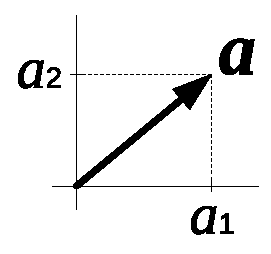
\includegraphics[keepaspectratio, width=3.1cm,height=3cm,clip]{chap9_ookisa001.pdf}
                \caption{2次元ベクトルの大きさ}
                \label{fig:chap9_ookisa001}
            \end{center}
        \end{figure}

        \subsection{基本演算}
        複数のベクトルがあるとき,ベクトル同士の演算を定義しておこう.
        ベクトルに対して定義される演算は,加算と減算と乗算であり,
        除算は定義されない.乗算には,
        定数倍,内積(スカラー積),外積(ベクトル積)の3種類がある.
        しかし,ここで言うベクトルの乗算は,
        普通の数で行われる乗算とは異なる概念であることに注意されたい
            \footnote{
                違いは,この後の説明で,自ずとわかるはず.
            }.
        ベクトルの演算が定義できるのは,すべてのベクトルの次元が同じ場合に限る.
        以下のベクトル演算の定義にでてくるベクトルは,すべて $n$ 次元
        ベクトルであると仮定する.次元が異なるベクトル同士の演算は定義しない.

        数学的な演算公理を示すことはせず,直感的にわかりやすい表現で
        演算の定義を示すにとどめておこう.

        \subsubsection{加算}
        2つの $n$ 次元ベクトル $\ba$,$\bb$ があるとき,
        この2つのベクトルに対する演算 $\ba+\bb$ を \textbf{加算} といい,
        次のように定義する.
        \begin{align}
            \ba + \bb   &:= (a_{1},\, a_{2},\,\cdots,\,a_{n}) + (b_{1},\,b_{2},\,\cdots,\, b_{n}) \notag \\
                        &=  (a_{1}+b_{1},\, a_{2}+b_{2},\,\cdots,\, a_{n}+b_{n} ).
        \end{align}

        成分を示す場合には,次のようになる.
        \begin{align}
            {(\ba+\bb)}_{i} := a_{i}+b_{i} \quad,\quad (i=1,\,2,\,\cdots,\,n).
        \end{align}
        添字の $i$ はベクトルの成分番号を示している記号である.式はすべての成分で
        成り立つが,すべての成分を書くと,上の定義のように,$i=1,\,2,\,\cdots,\,n$ の $n$ 通り
        を記述する必要が出てくる.しかし,どの成分番号に対しても,同じ形の式で
        定義で定義されることから,1から$n$の任意の一つを代表的に表す $i$ を導入した.

        \subsubsection{定数倍}
        スカラー $k$ と $n$ 次元ベクトル $\ba$ の積 $k\ba$ を \textbf{定数倍} といい,
        次で定義する.ここでは,$k$ を実数とする.
        \begin{align}
            k\ba := (k{a}_{1},\, k{a}_{2},\, \cdots,\, k{a}_{n}).
        \end{align}
        $\ba$ のすべての成分を $k$ 倍するということである.

        成分を示す場合には,次のように書く.
        \begin{align}
            {(k\ba)}_{i} := k{a}_{i} \quad,\quad  (i=1,\,2,\,\cdots,\,n).
        \end{align}

        \subsubsection{減算}
        加算と定数倍を定義しておけば,減算を定義する必要はない
            \footnote{
                一方に$-1$を乗じて(乗算)から,たし合わせればいい(加算).
            }.
        しかし,特徴的な演算であるため,この演算に \textbf{減算} という呼称を与える.
        減算は以下のような演算でのことをいう.2つの $n$ 次元ベクトル $\ba$,$\bb$ があるとき,
        ベクトルの減算 $\ba-\bb$ とは,
        \begin{align*}
            \ba-\bb &:= \ba + (-1)\bb \\
                    &= (a_{1}+(-1)b_{1},\, a_{2}+(-1)b_{2},\,\cdots,\, a_{n}+(-1)b_{n} ) \\
                    &= (a_{1}-b_{1},\, a_{2}-b_{2},\,\cdots,\, a_{n}-b_{n} )
        \end{align*}
        のような演算のことである.

        成分を示す場合には,次のようになる.
        \begin{align}
            {(\ba-\bb)}_{i} := a_{i}-b_{i} \quad,\quad (i=1,\,2,\,\cdots,\,n).
        \end{align}

        \subsubsection{内積(スカラー積)}
        2つの$n$次元ベクトル $\ba$,$\bb$ の内積 $\ba\cdot\bb$ とは,以下の演算のことをいう.
        \begin{align}\label{eq:chap9_naiseki001}
            \ba\cdot\bb := \sum_{i=1}^{n} a_{i}b_{i}.
        \end{align}

        展開したほうが,見やすいかもしれない(同じことを書いているだけ).
        \begin{align}
            \ba\cdot\bb := a_{1}b_{1} + a_{2}b_{2} + \cdots + a_{n}b_{n}.
        \end{align}

        演算結果がスカラーになることから,\textbf{スカラー積} ということもある.

        2次元ベクトルの場合,内積には図形的なイメージがある.
        それを強調した場合の,内積の定義は以下の通り.
        \begin{align}
            \ba\cdot\bb := |\ba||\bb| \cos \theta.
        \end{align}
        この定義は上の式(\ref{eq:chap9_naiseki001})の $n=2$ の場合と同値である.
        証明は後回し.
        \begin{figure}[htbp]
            \begin{center}
                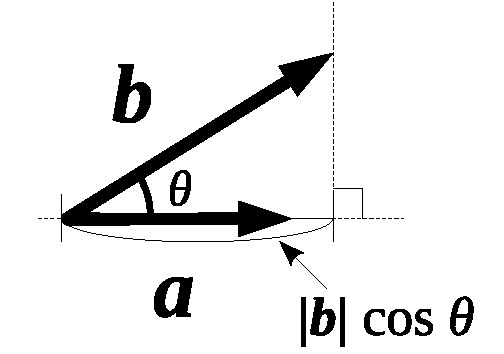
\includegraphics[keepaspectratio, width=4.23cm,height=3cm,clip]{chap9_naiseki001.pdf}
                \caption{内積}
                \label{fig:chap9_naiseki001}
            \end{center}
        \end{figure}

        \subsubsection{外積(ベクトル積)}
            \begin{mysmallsec}{外積の定義}
                2つの3次元ベクトル $\ba$,$\bb$ からなるベクトルの \textbf{外積} を
                $\ba\times\bb$ と表し,以下でその演算を定義する.
                    \begin{align*}
                            \ba \times \bb &:=& (\,
                                    a_{2}b_{3} - a_{3}b_{2},\;
                                    a_{3}b_{1} - a_{1}b_{3},\;
                                    a_{1}b_{2} - a_{2}b_{1}
                                \,)
                    \end{align*}

                演算結果がベクトルであることから,\textbf{ベクトル積} ということもある.

                唐突な定義で,無味乾燥だと思われるかもしれないが,
                根拠のあるものである.それを以下で説明しよう.
            \end{mysmallsec}

            \begin{mysmallsec}{一言}
                ベクトルの外積はわかりにくい.実際,定義式が少々複雑であり,図形的な
                イメージをすぐに描くには難しいかもしれない.しかし,ここを少々辛抱して
                手計算による練習をいくらかすることで,ベクトルの外積の意味やイメージを
                つかめるようになるはずである.
                ここでは,ベクトルの外積の定義を示すと共に,イメージを少しでも早くつかむ
                ことができるよう,丁寧に説明していく
            \end{mysmallsec}

            \begin{mysmallsec}{3次元ベクトルの外積のみを扱う}
                ここでの興味は3次元ベクトルの外積である.他の次元の外積は考えない.
                "興味がない"というのが直接的な理由だけれど,
                外積は内積のように簡単に $n$ 次元に拡張することができないことも,
                知っておいて損はないかも(多次元に拡張しようとして無駄な時間を費やさないように).

                外積の拡張に興味があれば,\textbf{外積代数} を学んでみる良い.
                外積代数は,ここでいう外積の自然な拡張ではないが(定義から違う),
                外積計算を発展させた形式の数学であることは実感できるだろう.
            \end{mysmallsec}

            \begin{mysmallsec}{定義の意味すること}
                ベクトルの外積とは,与えられた2つのベクトルから,
                この2つのベクトルの方向から独立した
                新しい方向を持つベクトルを1つ生成する演算である.
                その新しいベクトルの方向とは,2つのベクトルの両方に直交する方向であり,
                その大きさは $|\ba||\bb|\sin \theta$ である.
            \end{mysmallsec}

            \begin{mysmallsec}{外積の定義を知識0から作ろう}
                外積の定義の意味を実感するには,回り道かもしれないが,
                外積の定義に至るまでの思考プロセスをたどるとよい.
                先に示した外積の定義を一度忘れて,外積を1から作っていこう.
            \end{mysmallsec}

            \begin{mysmallsec}{外積の定義の目的}
                なぜ外積を定義したいのか.その理由は,外積を定義することにより,
                ある物理現象の数学的扱いが可能になるからである.必要は発明の母.
                力の釣り合いの解析には外積が欠かせないし,電磁気学ではローレンツ力
                を表すのに使われる.外積は闇雲に定義された演算ではなく,自然現象を
                詳細に観測した結果,それを説明するのに必要な演算方法なのである.
                自然現象の一部にはある特別な規則があり,それを数式で表そうとして
                試行錯誤して組み立てられた数学的概念が,外積なのである.
            \end{mysmallsec}

            \begin{mysmallsec}{外積演算に要求されること}
                2つの3次元ベクトル $\ba$,$\bb$ から,外積
                    \footnote{
                        今は,演算の名前なんてどうでも良い.知りたいのは
                        その具体的な演算方法である.この演算名は便宜的に
                        使用するものであり,"新しい演算方法"という
                        意味程度で捉えてもらいたい.
                    }
                によって生成したいベクトルの条件は以下の通りだった.
                \begin{enumerate}
                    \item 方向は $\ba$ と $\bb$ の両方に直交する方向である
                    \item 大きさは,$|\ba||\bb| \sin \theta$
                \end{enumerate}

                つまり,これから考えることは,
                \begin{enumerate}
                    \item 方向は 2つのベクトルに直交するようなベクトルをどう作るか.
                    \item さらに大きさを,$|\ba||\bb| \sin \theta$ にするには,どういう制約必要か
                \end{enumerate}
                の2点である.
                    \begin{figure}[hbt]
                        \begin{center}
                            \includegraphicslarge{gaiseki_01.pdf}
                            \caption{外積のイメージ}
                            \label{fig:gaiseki_01}
                        \end{center}
                    \end{figure}
            \end{mysmallsec}

            \begin{mysmallsec}{要求されることから,条件式を導く}
                2つの3次元ベクトル $\ba$,$\bb$ から,外積
                そのようなベクトルが仮に存在できたとして,それを $\bc$ と
                表すことにしよう($\bc:=\ba\times\bb$).

                $\bc$ は $\ba$ と $\bb$ の両方に直交しているから,内積が0になっているはずである
                    \footnote{
                        $\ba$,$\bb$ はともにゼロベクトルでないので(最初に要請される条件),
                        $|\ba| \neq 0$ ,$|\bb| \neq 0$ だから,$\cos(\pi/2)=0$ が
                        成立していなければならない.
                        $\ba$,$\bb$ の少なくとも一方がゼロベクトルである場合も外積は定義されるが,
                        この場合,新たに生成されるベクトルもゼロベクトルとなる特別な場合である.
                    }.

                したなら,次式が成立してなければならない.すなわち,
                    \begin{align*}
                        \ba \cdot \bc &= |\ba||\bc| \cos \frac{\pi}{2} = 0 \\
                        \bb \cdot \bc &= |\bb||\bc| \cos \frac{\pi}{2} = 0
                    \end{align*}
                である.
                ベクトル $\bc$ の成分を $(\,c_{1}\,,c_{2}\,,c_{3}\,)$ としよう.
                $\ba$ と $\bb$ についても同様に,
                それぞれ,$(\,a_{1}\,,a_{2}\,,a_{3}\,)$,
                $(\,b_{1}\,,b_{2}\,,b_{3}\,)$ とする.
                そうすると,上の2つの式は,また,以下のよう書いても同じことである.
                すなわち,
                    \begin{align*}
                        a_{1}c_{1} + a_{2}c_{2} + a_{3}c_{3} &= 0. \\
                        b_{1}c_{1} + b_{2}c_{2} + b_{3}c_{3} &= 0.
                    \end{align*}

                ベクトルの方向については,上の2式が成り立つことがその
                条件であるが,向きについては何も言っていない.
                そこで,次のように向きを決めてしまおう.すなわち,
                    \begin{description}
                        \item[向きの定義]
                            ベクトル $\ba$ とベクトル $\bb$ から生成する
                            外積 $\bc$ のむきは,
                            $\ba$ から $\bb$ に 向かって右ねじを右まわし回したときに,ネジが進む向きを,正方向とする.
                            これを満たすことを,\textbf{右手系をなす} という
                            別名「右ねじの法則」という表現が使われることも多い.
                    \end{description}

                    \begin{figure}[hbt]
                        \begin{center}
                            \includegraphicsdefault{migineji_01.pdf}
                            \caption{右ねじを回して進む方向}
                            \label{fig:migineji_01}
                        \end{center}
                    \end{figure}

                ベクトルにはもうひとつの性質である大きさ
                も考えないといけない.どのような大きさにしようと自由だが,
                最も簡潔に大きさを定めたい.もとの2つのベクトル $\ba$,$\bb$ より,
                この二つのベクトルが張る平行四辺形の面積を,その大きさと
                するのが最も簡単だろう.実際,数学的にもこのような定義が
                なされる.これが最も無理のない定義なのだろう.すると,
                $\bc$ の条件として,次式も加わることになる.
                    \begin{align*}
                        |\bc| &= | \ba || \bb | \sin\theta \\
                        &\Leftrightarrow \quad
                        \sqrt{{c_{1}}^{2}+{c_{2}}^{2}+{c_{3}}^{2}}
                        =
                        \sqrt{{a_{1}}^{2}+{a_{2}}^{2}+{a_{3}}^{2}}
                        \sqrt{{b_{1}}^{2}+{b_{2}}^{2}+{b_{3}}^{2}}
                        \sin\theta
                    \end{align*}

                これで,都合3つの条件式と,向きの定義は揃った.もう一度,まとめて書いておこう.
                \\
                \begin{itembox}[a]{外積演算で満たすべき条件式}
                    外積演算では,以下の条件式を満たさねばならない.
                    \begin{description}
                        \item[(1)] $a_{1}c_{1} + a_{2}c_{2} + a_{3}c_{3} = 0$ ($\bc \perp \ba$)
                        \item[(2)] $b_{1}c_{1} + b_{2}c_{2} + b_{3}c_{3} = 0$ ($\bc \perp \bb$)
                        \item[(3)] $\sqrt{{c_{1}}^{2}+{c_{2}}^{2}+{c_{3}}^{2}}
                               = \sqrt{{a_{1}}^{2}+{a_{2}}^{2}+{a_{3}}^{2}}
                                 \sqrt{{b_{1}}^{2}+{b_{2}}^{2}+{b_{3}}^{2}}
                                 \sin\theta$ (大きさ)
                        \item[(4)] $\ba,\,\bb,\,\bc$ は右手系をなす.(向き)
                    \end{description}
                \end{itembox}
                \\

                未知数が $c_{1}$,$c_{2}$,$c_{3}$ と三つなのに対し,
                条件式も同じく3つであり,数式的な条件としては必要十分である
                    \footnote{
                        これで,大きさと方向を定めることができる.
                    }.
                また,ベクトルの向きの定義もした.これで,外積を作る準備が
                整った.あとは,外積を作れるかどうか,言い換えれば,このように
                定義した外積というものが存在可能かどうかを,確認すれば良い.
            \end{mysmallsec}

            \begin{mysmallsec}{外積の成分表示}
                このような3式
                    \footnote{
                        正確には,「3つの式と,向きの定義」と書くべきだけど,
                        向きは人間が勝手に選ぶものなので,数式的に気にするもの
                        ではない.
                    }
                を満たすような $\bc$ は存在するのか.存在するとしたら,
                その成分はどのようになるか.それをこれから考えていこうと思う.それで,
                どうやって求めるかなんだけど,その方法は幾つか思い当たる.
                式をくどくどと計算をして発見的に答えを得る方法もあるけれど,
                それだと少々話が長くなり,計算も面倒くさい.なので,この問題の
                答えはすでに得られていることだから,先に答えを見てしまおう.
                そのほうが早い.

                で,その答えとは,
                    \begin{align*}
                        \bc &= (\,c_{1},\,c_{2},\,c_{3}\,) \\
                            &= (\,
                                    a_{2}b_{3} - a_{3}b_{2},\;
                                    a_{3}b_{1} - a_{1}b_{3},\;
                                    a_{1}b_{2} - a_{2}b_{1}
                                \,)
                    \end{align*}
                である.なにやら複雑な式に見えるが,次のように書くと,
                ある規則がみえてくるだろう.
                    \begin{align}\label{eq:VecGaiseki_Seibun}
                        \bc =
                        \left[
                            \begin{array}{c}
                                c_{1} \\
                                c_{2} \\
                                c_{3} \\
                            \end{array}
                        \right]
                        =
                        \left[
                            \begin{array}{c}
                                a_{2}b_{3} - a_{3}b_{2} \\
                                a_{3}b_{1} - a_{1}b_{3} \\
                                a_{1}b_{2} - a_{2}b_{1} \\
                            \end{array}
                        \right].
                    \end{align}

                $\ba$,$\bb$ の成分の添字を縦方向に意識して眺めると,
                巡回($1 \to 2 \to 3 \to 1$)しているのが見える
                    \footnote{
                        複雑そうに見えるけど,規則さえ分かってしまえば,
                        覚えるのはたやすい.最初の $a_{2}b_{3}$ さえ覚えてしまえば,
                        残りは機械的に記述できる.引く数は添字の数字を入れ替えた
                        ものだし,その他の成分については添字を巡回させればいい.
                    }.
                式(\ref{eq:VecGaiseki_Seibun})は,
                先ほど上げた3つの条件式を必要十分に満たす.
            \end{mysmallsec}

            \begin{mysmallsec}{外積の成分表示の検算}
                式(\ref{eq:VecGaiseki_Seibun})が本当に条件を満たすかどうかを,
                確かめておこう.まず,$\bc \perp \ba$,$\bc \perp \bb$ を
                満たすことを示す.やり方は,単純に条件式に成分を代入して,
                式を整理するだけである.

                条件式(1)について,
                    \begin{align*}
                         &a_{1}c_{1} + a_{2}c_{2} + a_{3}c_{3} \\
                         &\qquad=   a_{1}(a_{2}b_{3} - a_{3}b_{2})
                             + a_{2}(a_{3}b_{1} - a_{1}b_{3}) + a_{3}(a_{1}b_{2} - a_{2}b_{1}) \\
                         &\qquad=   a_{1}a_{2}b_{3} - a_{1}a_{3}b_{2}
                             + a_{2}a_{3}b_{1} - a_{2}a_{1}b_{3} + a_{3}a_{1}b_{2} - a_{3}a_{2}b_{1} \\
                         &\qquad= 0.
                    \end{align*}

                条件式(2)も同じように計算できる.
                    \begin{align*}
                         &b_{1}c_{1} + b_{2}c_{2} + b_{3}c_{3} \\
                         &\qquad=   b_{1}(a_{2}b_{3} - a_{3}b_{2})
                             + b_{2}(a_{3}b_{1} - a_{1}b_{3}) + b_{3}(a_{1}b_{2} - a_{2}b_{1}) \\
                         &\qquad=   b_{1}a_{2}b_{3} - b_{1}a_{3}b_{2}
                             + b_{2}a_{3}b_{1} - b_{2}a_{1}b_{3} + b_{3}a_{1}b_{2} - b_{3}a_{2}b_{1} \\
                         &\qquad= 0.
                    \end{align*}

                たしかに,二つの条件式を満たしている.このことにより,
                ベクトル $\bc$ は,ベクトル $\ba$,$\bb$ に直交している
                ことが確かめられた.つまり,ベクトル $\bc$ の方向は
                条件に沿うものであると言える.

                では,残りの大きさに関する条件式について,それを満たすか
                を計算してみよう.もう一度,大きさを決める条件式(3)を
                書くと,
                    \begin{align*}
                        &\sqrt{{c_{1}}^{2}+{c_{2}}^{2}+{c_{3}}^{2}}
                        =
                        \sqrt{{a_{1}}^{2}+{a_{2}}^{2}+{a_{3}}^{2}}
                        \sqrt{{b_{1}}^{2}+{b_{2}}^{2}+{b_{3}}^{2}}
                        \sin\theta
                    \end{align*}
                でるが,両辺を2乗して,
                    \begin{align*}
                        {c_{1}}^{2}+{c_{2}}^{2}+{c_{3}}^{2}
                        =
                        \left({a_{1}}^{2}+{a_{2}}^{2}+{a_{3}}^{2}\right)
                        \left({b_{1}}^{2}+{b_{2}}^{2}+{b_{3}}^{2}\right)
                        {\sin}^{2}\theta.
                    \end{align*}
                ここで,三角関数の公式 ${\sin}^{2}\theta + {\cos}^{2}\theta = 1$ を
                思い起こし,${\sin}^{2}\theta = 1 - {\cos}^{2}\theta $ と置き換えて,
                    \begin{align*}
                        &{c_{1}}^{2}+{c_{2}}^{2}+{c_{3}}^{2} \\
                        &\quad =    \left({a_{1}}^{2}+{a_{2}}^{2}+{a_{3}}^{2}\right)
                                    \left({b_{1}}^{2}+{b_{2}}^{2}+{b_{3}}^{2}\right)
                                    \left(1 - {\cos}^{2}\theta \right) \\
                        &\quad =    \left({a_{1}}^{2}+{a_{2}}^{2}+{a_{3}}^{2}\right)
                                    \left({b_{1}}^{2}+{b_{2}}^{2}+{b_{3}}^{2}\right) \\
                                    &\quad \qquad -\left({a_{1}}^{2}+{a_{2}}^{2}+{a_{3}}^{2}\right)
                                        \left({b_{1}}^{2}+{b_{2}}^{2}+{b_{3}}^{2}\right)
                                        {\cos}^{2}\theta.
                    \end{align*}
                最後の行の
                    \begin{equation*}
                        \left({a_{1}}^{2}+{a_{2}}^{2}+{a_{3}}^{2}\right)
                        \left({b_{1}}^{2}+{b_{2}}^{2}+{b_{3}}^{2}\right)
                        {\cos}^{2}\theta.
                    \end{equation*}
                に注目すると,
                    \begin{align*}
                        &\left(
                            \sqrt{{a_{1}}^{2}+{a_{2}}^{2}+{a_{3}}^{2}}
                            \sqrt{{b_{1}}^{2}+{b_{2}}^{2}+{b_{3}}^{2}}
                            {\cos}\theta
                        \right)^{2} \\
                            &\qquad=
                            \left(
                                \ba \cdot \bb
                            \right)^{2} \\
                            &\qquad=
                            \left(
                                a_{1}b_{1}+a_{2}b_{2}+a_{3}b_{3}
                            \right)^{2}.
                    \end{align*}

                つまり,大きさの定義式は以下のように書き換えられる.
                    \begin{align*}
                        &{c_{1}}^{2}+{c_{2}}^{2}+{c_{3}}^{2} \\
                        &\qquad =   \left({a_{1}}^{2}+{a_{2}}^{2}+{a_{3}}^{2}\right)
                                    \left({b_{1}}^{2}+{b_{2}}^{2}+{b_{3}}^{2}\right)
                                    \left(1 - {\cos}^{2}\theta \right) \\
                        &\qquad =   \left({a_{1}}^{2}+{a_{2}}^{2}+{a_{3}}^{2}\right)
                                    \left({b_{1}}^{2}+{b_{2}}^{2}+{b_{3}}^{2}\right)
                                    -   \left(
                                            a_{1}b_{1}+a_{2}b_{2}+a_{3}b_{3}
                                        \right)^{2}.
                    \end{align*}

                この式を,ベクトル $\bc$ が満たしていることを確認すればよい.
                    \begin{align*}
                        |\bc|^{2}
                        &=
                        {c_{1}}^{2}+{c_{2}}^{2}+{c_{3}}^{2} \\
                        &=
                         {(a_{2}b_{3} - a_{3}b_{2})}^{2}
                         + {(a_{3}b_{1} - a_{1}b_{3})}^{2}
                         + {(a_{1}b_{2} - a_{2}b_{1})}^{2} \\
                        &=
                        \left(
                            {a_{2}}^{2}{b_{3}}^{2} + {a_{3}}^{2}{b_{2}}^{2} - 2a_{2}a_{3}b_{2}b_{3}
                        \right)
                        + \left(
                            {a_{3}}^{2}{b_{1}}^{2} + {a_{1}}^{2}{b_{3}}^{2} - 2a_{1}a_{3}b_{1}b_{3}
                        \right) \\ &\qquad
                        + \left(
                            {a_{1}}^{2}{b_{2}}^{2} + {a_{2}}^{2}{b_{1}}^{2} - 2a_{1}a_{2}b_{1}b_{2}
                        \right) \\
                        &=
                          {a_{2}}^{2}{b_{3}}^{2} + {a_{3}}^{2}{b_{2}}^{2} + {a_{3}}^{2}{b_{1}}^{2}
                        + {a_{1}}^{2}{b_{3}}^{2} + {a_{1}}^{2}{b_{2}}^{2} + {a_{2}}^{2}{b_{1}}^{2} \\
                        &\quad - 2a_{2}a_{3}b_{2}b_{3} - 2a_{1}a_{3}b_{1}b_{3} - 2a_{1}a_{2}b_{1}b_{2} \\
                        &=
                          \left({a_{1}}^{2}{b_{3}}^{2} + {a_{1}}^{2}{b_{2}}^{2}\right)
                        + \left({a_{2}}^{2}{b_{3}}^{2} + {a_{2}}^{2}{b_{1}}^{2}\right)
                        + \left({a_{3}}^{2}{b_{2}}^{2} + {a_{3}}^{2}{b_{1}}^{2}\right) \\
                        &\quad - 2a_{2}a_{3}b_{2}b_{3} - 2a_{1}a_{3}b_{1}b_{3} - 2a_{1}a_{2}b_{1}b_{2}.
                    \end{align*}

                ちょっと一息.まだまだ式変形は続く.ちなみに,上式の冗長な括弧は,
                以降の式変形のために,明示的に記述している.

                次に,トリッキーな作業をする.それは,ある数 $x$ に対して,
                当然,$0=x-x$ が成り立つから,0を加えるということは $x-x$ を加えることと同じである.
                そして0を加えても等式は成り立つ.
                この考え方を利用して,式変形を続けよう.
                    \begin{align*}
                        |\bc|^{2}
                        &= {a_{1}}^{2}{b_{3}}^{2} + {a_{1}}^{2}{b_{2}}^{2}
                            + \left({a_{1}}^{2}{b_{1}}^{2} - {a_{1}}^{2}{b_{1}}^{2}\right) \\
                        &\quad + {a_{2}}^{2}{b_{3}}^{2} + {a_{2}}^{2}{b_{1}}^{2}
                            + \left({a_{2}}^{2}{b_{2}}^{2} - {a_{2}}^{2}{b_{2}}^{2}\right) \\
                        &\quad + {a_{3}}^{2}{b_{2}}^{2} + {a_{3}}^{2}{b_{1}}^{2}
                            + \left({a_{3}}^{2}{b_{3}}^{2} - {a_{3}}^{2}{b_{3}}^{2}\right) \\
                        &\quad - 2a_{2}a_{3}b_{2}b_{3} - 2a_{1}a_{3}b_{1}b_{3} - 2a_{1}a_{2}b_{1}b_{2} \\
                        &=   {a_{1}}^{2}\left({b_{1}}^{2} + {b_{2}}^{2} + {b_{3}}^{2}\right)
                           + {a_{2}}^{2}\left({b_{1}}^{2} + {b_{2}}^{2} + {b_{3}}^{2}\right)
                           + {a_{3}}^{2}\left({b_{1}}^{2} + {b_{2}}^{2} + {b_{3}}^{2}\right) \\
                        &\quad -{a_{1}}^{2}{b_{1}}^{2} - {a_{2}}^{2}{b_{2}}^{2} - {a_{3}}^{2}{b_{3}}^{2}
                               - 2a_{2}a_{3}b_{2}b_{3} - 2a_{1}a_{3}b_{1}b_{3} - 2a_{1}a_{2}b_{1}b_{2} \\
                        &=  \left( {a_{1}}^{2} + {a_{2}}^{2} + {a_{3}}^{2} \right)
                            \left( {b_{1}}^{2} + {b_{2}}^{2} + {b_{3}}^{2} \right)
                           -\left(a_{1}b_{1}+a_{2}b_{2}+a_{3}b_{3}\right)^{2}.
                    \end{align*}

                式変形が長々と続いたが,これでやっと確かめられた
                \footnote{
                    以下の恒等式が成立している.
                        \begin{equation*}
                            \left( X + Y + Z \right)^{2}
                            = {x}^{2} + {y}^{2} + {z}^{2} + 2XY + 2YZ + 2ZX.
                        \end{equation*}
                    ここでは,$X=a_{1}b_{1}$,$Y=a_{2}b_{2}$,$Z=a_{3}b_{3}$ に対応している.
                }.

                条件式(4)は,条件式(1)(2)(3)では特定することのできなかった向きを
                人為的に定めるものである.うるさいことを言うと,条件式(4)が条件式(1)(2)(3)に
                矛盾しないことを示すべきだが,割愛する.どちらの向きを正とするか,という問題
                であり,大げさに議論するところではない.単なる取り決めである.

                以上から,$\bc$ は3つの条件式を満たすことが確かめられ,ベクトルの外積が
                存在することが示された.つまり,ベクトルの外積は定義可能であることが確かめられた.
            \end{mysmallsec}

            \begin{mysmallsec}{最後に一言}
                何度も言うが,ベクトルの外積は導かれるものではない.人の想像力によって
                定義するものである.この外積という概念を導入することで,物体の回転を数学的に
                扱うことができるのである.というか,実際は話が逆で,ベクトルの外積の定義に従う
                物理現象が発見され,この現象を数学的に扱うことができるように,外積が定義される
                のである.もしかしたら,外積の定義が突拍子も無いと感じているかも知れないが,
                現実に外積を用いて説明される物理現象が生じているのである.外積はその現象を
                扱うために導入されるのだ.
            \end{mysmallsec}

                \begin{memo}{右手系とは何か}
                    外積の定義のうちの,向きの定義をもう一回読んでみよう.

                    \begin{description}
                        \item[向きの定義]
                            ベクトル $\ba$ とベクトル $\bb$ から生成する
                            外積 $\bc$ のむきは,
                            $\ba$ から $\bb$ に 向かって右ねじを右まわし回したときに,ネジが進む向きを,
                            正方向とする.これを満たすことを,\textbf{右手系をなす} という.
                    \end{description}


                    なぜこのように定義するのかという疑問があろうが,この疑問
                    はすぐに捨て去るべきだ.なにしろ,答えがないのだから.
                    しかし,天下り的な説明はよくない.なので,できるだけ
                    “もっともらしい”説明を,以下に記述しておくことにしよう
                        \footnote{
                            あくまでも,“もっともらしく”記述するのであり,
                            これがほんとうの理由だとか,正解だとかというものではない.
                            天下り的な説明ではスッキリとせず,モヤモヤしてしまう
                            ので,これを少しでも解消できればと考えて,記述
                            するものである.
                        }.

                    2つのベクトル $\ba$,$\bb$ に直交する方向は内積の数式で表現され,
                    数学的に議論できるが,方向は計算で導くことはできない.なので,
                    予め,向きを定めておくのである.どちらの向きを正方向としても,
                    それ以降で変更しなければ,論理に矛盾は生じない.しかし,向きを
                    決めないと議論ができないので,人為的な向きの定義を施すのである.

                    では,なぜ,「右ネジをまわして進む向き」と表現するのか.
                    これにも,多分,明確な答えはない.
                    おそらく,これが最も簡潔な言い回しで,誤解なく,加えて直感的イメージ
                    しやすく説明できるからだろう.しかし,学術的には格好をつけて,
                    「右手系をなす」と言われる.それは,右手の親指を人差し指に近づけるという
                    行為が,親指を右まわしするという行為に当たり,中指の先の向きが
                    外積の向きに一致するからである.元となる2つのベクトルが親指と人差し指に
                    値し,それに直交する向きに中指が向いているのだ.
                    \begin{figure}[hbt]
                        \begin{tabular}{cc}
                            \begin{minipage}{0.5\hsize}
                                \begin{center}
                                    
\includegraphics[keepaspectratio, width=3cm,height=3.75cm,clip]{migitekei_TE_2.pdf}

                                    (a) 右手
                                    \label{fig:migitekei_TE_mono_x}
                                \end{center}
                            \end{minipage}
                            \begin{minipage}{0.5\hsize}
                                \begin{center}
                                    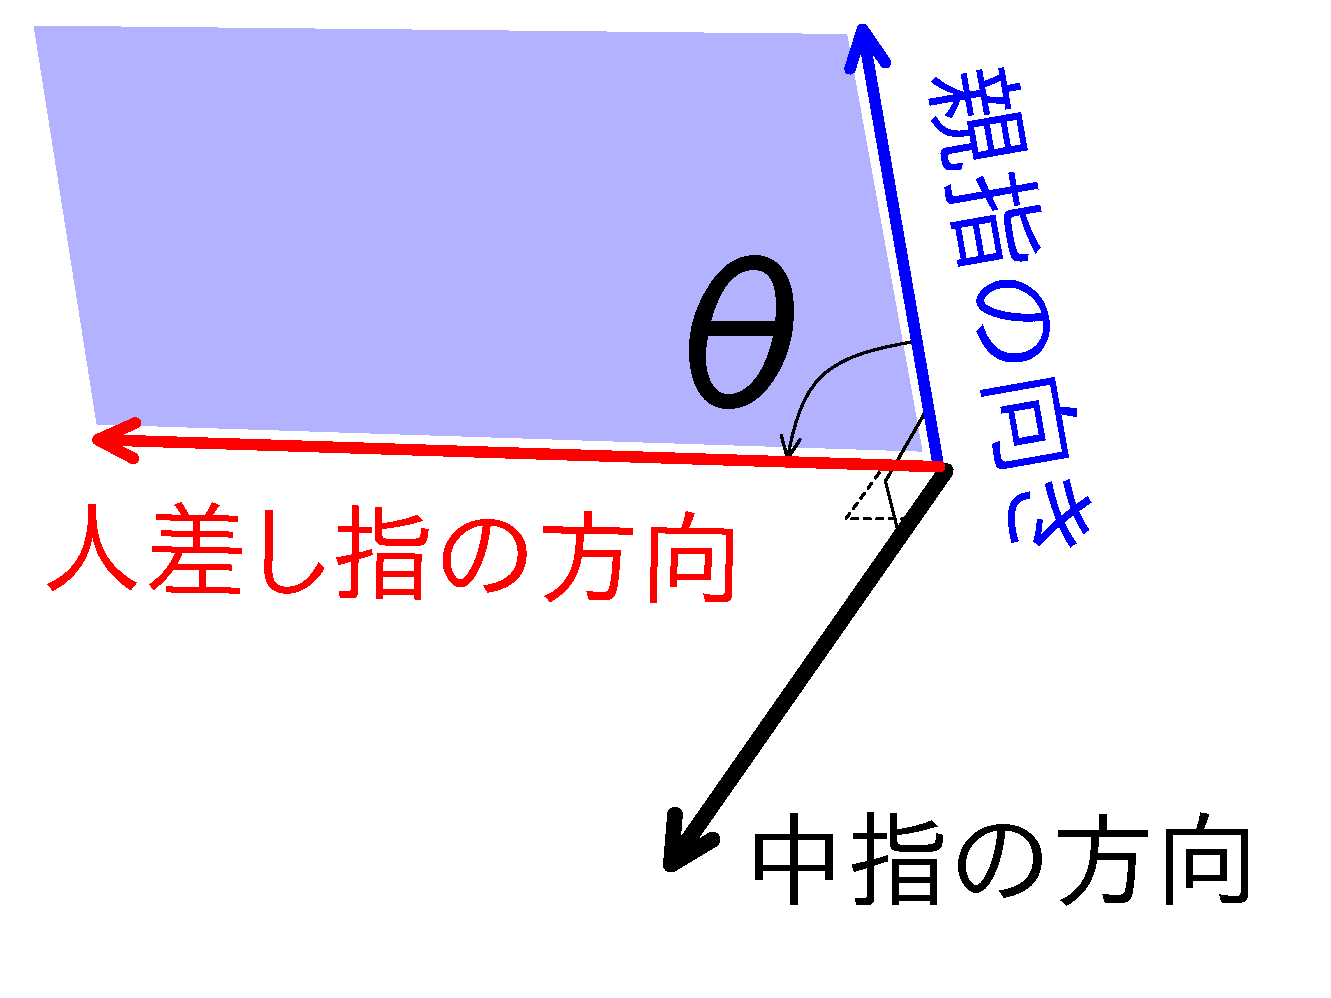
\includegraphics[keepaspectratio, width=3cm,height=3.75cm,clip]{migineji_Myhand.pdf}

                                    (b) 対応図
                                    \label{fig:migineji_Myhand}
                                \end{center}
                            \end{minipage}
                        \end{tabular}
                        \caption{右手系}
                    \end{figure}
                \end{memo}

        \subsubsection{乗算?}
            ベクトルの乗算を,加算と同じように定義できないだろうか.
            つまり,2つの $n$ 次元ベクトル $\ba=(a_{1},\,a_{2},\,\cdots,\,n)$,
            $\bb=(b_{1},\,b_{2},\,\cdots,\,n)$ を用いて,
                \begin{equation*}
                    {(\ba \ast \bb)}_{i} = a_{i}b_{i}
                \end{equation*}
            と定義してはだめか
                \footnote{
                    記号に $\ast$ を使った理由は,内積の記号に $\cdot$,
                    外積の記号に $\times$ が使われるため,これらと区別
                    したかったためである.
                }.
            先人がこのように定義をしていないからには,
            できない理由があるに違いない.しかし,このように
            乗算を定義しても,不整合が起きるわけでもなく,定義不可能
            とは思えず,むしろ定義可能であると思えて仕方ない.
            私の力では,この定義を採用しない強い理由を見つけられない.

            しかし,このような乗算を定義してしまうと,ベクトルと数の違いが全く
            なくなってしまうことは確かだ
                \footnote{
                    実際に試してみてほしい.数と全く同じで,ベクトルを
                    定義した意味が全く感じられないことだろう.
                }.
            つまり,ベクトルとは表記上の利便性が向上
            しただけで,数学的な新しい概念となるわけではなくなる.
            数学的な発展を考えた場合,このような仕方の冗談の定義では
            前進がないので無駄ということになる.要するに,こんな乗算を定義
            してしまっては,わざわざベクトルを定義したことが無意味になって
            しまうのだ.表記方法を工夫しただけで新しい数学的概念とは言えない.
            もちろんこれでは,物理学にとっても,何のご利益もない
            ものになってしまうことだろう.
            だから,むしろ意識的に,このような定義を避けているのではない
            かと思われる(確証はない).ベクトルに内積や外積を定義することで,
            物理学に有用な数学になると共に,とても興味深い数学的対象となる.

        \subsubsection{除算??}
            ベクトルの内積の定義を採用すると,
            ベクトルの除算を定義することは難しい,と悟るのは容易だろう
            \footnote{
                $\bX\cdot\ba=k$ のとき,単純に $\ba=k/\bX$ とはできそうにない.
                $\bX$ をベクトルの変数とみなしたときに,この式を満たす $\bX$ は
                無限に存在するするから,できるとするならば,何か条件や約束事が必要だが,
                いい案は思い当たりそうにない.例えば,無限に存在する解をひとまとめにして,
                "解空間"(微分方程式など解空間とはべつもの)なるものをでっち上げたとしても,
                これ以上の発展は見込めないだろう.
            }.

            上記の "$\ast$" 乗算が採用されるのであれば,同じように除算を
            定義することは可能である.それは単に数を並べただけなので,
            吸うと全く同じ四則演算を定義すれば,不整合は起こらない.
            上記の乗算を定義しない理由に従うと,内積や外積を定義した方が
            学問的に有益である.そうなると,除算の定義が格段に難しくなる,
            というか,定義できたとしても条件が複雑すぎて,つまらなくなるだけだろう.

            だから,除算が定義できないのではなく,学問的に有益でないから定義しない
            と言ったほうが,正確なのであろう.

            数における0除算の禁止も,数学的に有益ではないから定義しないのだ,言えなくもない.
            よく挙げられる0除算が禁止される理由として,それを仮定すると不整合が起きるからだ
            といった説明がなされることがある
                \footnote{
                     $a$ を任意の数とするとき,$a \cdot 0 = 0$ が成立する(0の存在公理).
                     このとき,$a \neq b$ なる $b$ をもってきても $b \cdot 0 = 0$ である.
                     よって,$a \cdot 0 = b \cdot 0$(ここまでは正しい).
                     \textbf{両辺を0で割ると} $a=b$ となるが,これは $b$ の最初の条件に
                     矛盾する(不整合の発生).よって,0除算は禁止とされる.
                }.
            しかし,これは決して論理的な説明でない(美しい言い訳ではあるけれど).
            不整合が起きないように定義しなおせばよい.
            数学の論理は自然に存在するものではなく,人間が勝手気ままに構築
            するものであるから,定義なんていくらでも好き勝手できるはずである.ただ,
            0除算が定義できるようなうまい約束事を見つけられたとしても,複雑怪奇な理論
            が出来上がることになるのだろう(そんな理論に誰が興味を持つだろうか).

        \subsection{分解}
        1つのベクトルを複数のベクトルに分割することも可能である.
        例えば,$\ba = \bb + \bc$ が 成立しているとき,
        ベクトル $\ba$ は 2つのベクトル$\bb$と$\bc$に分割可能である.
        等式が成立していれば,分割するベクトルの個数に際限はない.
        このように,1つのベクトルを,加算が成り立つように複数のベクトルに
        分割することを,ベクトルの \textbf{分解} という.

        \subsection{単位ベクトル}
        大きさが1のベクトルを \textbf{単位ベクトル} という.
        単位ベクトルの記号は教科書により様々である.
        このノートでは,$\bn$ を単位ベクトルの記号として使用する
        \footnote{
            ただし,常にこの記号を用いるわけではない.その場合は,その直前か直後
            に説明を書くこととする.
        }.

        定義から,以下が成立する($n$ 次元を想定).
        \begin{align}
            |\bn| = \sqrt{\sum_{n=1}^{n} {n_{i}}^{2}} = 1.
        \end{align}
        $n_{i}$ のそれぞれの値には興味はないが,上記の関係式を満たす.
        単位ベクトルの方向は問わない.

                \subsection{演算の諸性質(公式)}
        \begin{mycomment}
            ベクトル基本的な演算性質を記しておく.
            $\ba$,$\bb$,$\bc$,$\bd$ はベクトルで,$k$,$l$ はスカラーである.
            括弧の内部の計算は,それがない部分よりも,優先度が高い(先に計算すべき)とし,
            それ以外の計算は左から順に計算する.
        \end{mycomment}

        \subsubsection{加算と定数倍に関する公式}
            ベクトルの加算と定数倍に関する演算性質は,スカラーの場合と変わらない.
            代表的な演算を以下に書いておく.
            \begin{enumerate}
                \item $\ba + \bb = \bb + \ba$
                \item $(\ba + \bb ) +\bc = \ba + (\bb + \bc)$
                \item $k (\ba + \bb) = k\ba + k\bb$
                \item $k(l\ba) = l(k\ba) =(kl)\ba$
                \item $\ba = \ba + \bzero = \bzero + \ba$
                \item $\ba +(-1)\ba = \bzero$
                \item $1\ba = \ba$
            \end{enumerate}

            以下,簡単に説明を与えておく.
            \begin{enumerate}
                \item 項の順序を入れ替えてから加算しても,結果は変わらない.\textbf{交換法則} とよばれる.
                \item 加算の順番を入れ替えても,結果は変わらない.\textbf{結合法則} とよばれる.
                \item 加算と定数倍に関する性質.
                      加算してから定数倍しても,両者を定数倍してから加算しても,どちらも
                      同じ結果になる.\textbf{分配法則} とよばれる.
                \item スカラーのかける順番を変えても,結果はわらなない.
                \item ゼロベクトル $\bzero$ を足しても結果は変わらない.
                      法則ではなく,$\bzero$ の存在を認めるもの.
                \item ベクトルから自身を引くとゼロベクトルになる.
                      $(-1)\ba$ は $\ba$ の \textbf{逆ベクトル} という.
                      $\ba$ も $(-1)\ba$ の逆ベクトルである(逆ベクトルの一意性).
                \item スカラーの1倍の1は記述を省略できる.
            \end{enumerate}

            どれも,定義から丁寧に計算すれば自明であるので,証明するまでもない
            \footnote{
                本音は$\cdots$
                \begin{itemize}
                    \item "記述が面倒だから省略させてほしい" という甘え
                    \item "書いたところで,ノートの記述が煩雑になって読みにくくなる" という言い訳
                    \item "自分で計算すれば,理解の確認になるのではないか" という逃げ
                \end{itemize}
                である.

                証明するには,式の両辺を独立に成分計算し,
                対応する成分同士が等しいことを確認すればいい.
                一意性を示したい場合には,異なる2つのものがあると仮定しても,
                両者が同値になることを示せばいい.
            }.

        \subsubsection{内積に関する公式}
            内積もスカラーと同じように扱える.主な性質は以下の通り.
            \begin{enumerate}
                \item $\ba \cdot \ba = {|\ba|}^{2}$
                \item $\ba \cdot \bb = \bb \cdot \ba$
                \item $\ba \cdot (\bb + \bc) = \ba \cdot \bb + \ba \cdot \bc$
                \item $(\ba + \bb) \cdot \bc = \ba \cdot \bc + \bb \cdot \bc$
                \item $k(\ba \cdot \bb) = (k\ba) \cdot \bb = \ba \cdot (k\bb)$
                \item $\ba \parallel \bb \Leftrightarrow \ba \cdot \bb = 0$
                \item $\ba \perp \bb \Leftrightarrow \ba \cdot \bb = \displaystyle\frac{\pi}{2}$
            \end{enumerate}

            言葉でも説明しておこう.
            \begin{enumerate}
                \item 自身の内積は,自身の大きさの2乗に等しい.
                \item 内積の項の順序を入れ替えても,結果は変わらない.
                \item 分配法則が成り立つ
                \item 分配法則の別の形(1と2より自明だろう)
                \item 定数倍と内積に関して,結合法則が成り立つ.
                \item 2つのベクトルが平行であることと,それらの内積が0であることは等価
                \item 2つのベクトルが垂直であることと,それらの内積が$\displaystyle\frac{\pi}{2}$であることは等価
            \end{enumerate}

            \begin{mysmallsec}{内積の使い所}
                物理学でベクトルの内積を使う場合は,2つのベクトルの交わりの角度を気にする場合が
                ほとんどである.平行なのか,垂直なのか,そうでなければどんな角度で交わっているのかが,
                内積の計算によってわかるからである.
            \end{mysmallsec}

        \subsubsection{外積に関する公式}
            外積の演算性質は,他とは異なるので,注意が必要である.
            \begin{enumerate}
                \item $\ba \times \ba = \bzero$
                \item $\ba \times \bb = - \bb \times \ba$
                \item $\ba \times (\bb \times \bc) = (\ba \cdot \bc) \bb - (\ba \cdot \bb) \bc $
            \end{enumerate}

            簡単にコメントを書いておく.
            \begin{enumerate}
                \item 自身の外積はゼロベクトルである.
                \item 外積の項の順序入れ替えると,符号が反転する.
                \item \textbf{ベクトルの三重積} という異名をもつ.
                      ちなみに,右辺の $\ba \cdot \bc$,$\ba \cdot \bb$ の演算結果はスカラーである.
            \end{enumerate}

            他にもたくさんあるけど,省略する.ベクトルの外積に関する公式は,
            一見して複雑な形をしたものが多く(検算が大変),挫折しがちだ.
            しばらく見ていると規則性が見えてきて,美しく感じるのかもしれないが,
            頻繁に使うのは上の3つくらいだ.後は,必要になったらときに,公式集を参照しよう.

        \subsubsection{単位ベクトルに関する公式}
        任意のベクトルは,同じ向きの単位ベクトルの定数倍である
            \footnote{
                証明はしないけど.
            }.
        アタリマエのことを言っているようだが,確認しておこう.
        ある $n$ 次元ベクトルを用意して,$\bX$ としよう.
        単位ベクトルの向きは,$\bX$ と同じとする.
        $\bX$ を単位ベクトル $\bn$ の定数 $k$ 倍と表せたとすると,$\bX = k\bn$ と
        なる.$\bX=(X_{1},\,X_{2},\,\cdots)$,$\bn=(n_{1},\,n_{2},\,\cdots,\,n)$ とすると,
            \begin{equation*}
                X_{i} = kn_{i} \quad,\quad (i=1,\,2,\,\cdots,\,n)
            \end{equation*}
        が成り立つ.これを踏まえて,$\bX$ の大きさ $|\bX|$を考えてみよう.
        簡単な計算で,$|\bX|=k$ が導ける.
            \begin{equation*}
                |\bX| = \sqrt{\sum_{n=1}^{n} {X_{i}}^{2}}
                      = \sqrt{\sum_{n=1}^{n} {(kn_{i})}^{2}}
                      = k \left(\sqrt{\sum_{n=1}^{n} {n_{i}}^{2}}\,\right)
                      = k \cdot 1
                      = k.
            \end{equation*}
        ここで,単位ベクトルの大きさが1であることを使用した.

        以上から,任意のベクトルは単位ベクトルを自身の大きさで定数倍したものに等しい,と言える.
        式で書くと,次の通り.
        \begin{align}
            \bX = |\bX|\bn.
        \end{align}

        上式を逆手に考えて,
        \begin{align}
            \bn = \frac{\bX}{|\bX|}= \frac{1}{|\bX|} \bX.
        \end{align}
        と見ることで,任意のベクトルの単位ベクトルを計算することもできる.

        しかし,次は無意味であることに注意しておくこと.
        \begin{align*}
            \mbox{(意味のない式)}\quad|\bX| = \frac{\bX}{\bn}
        \end{align*}
        ベクトル同士の除算は定義されておらず,この式は何も意味しない.


%%%        %======================================================================
%  Chapter : ベクトル解析
%  説明    : 電磁気学を記述する上で必要なベクトル解析のまとめ
%======================================================================

%======================================================================
%  Section
%======================================================================
    \section{ベクトル解析}
    \subsection{ベクトル変数(あるいは,変数ベクトル)}
    ベクトルには,スカラーにおける語彙「変数」に対応する,一般的呼称がない.
    ないと不便なので,このノートでは \textbf{ベクトル変数} という言い方を導入する.
    もしかしたら,\textbf{変数ベクトル} と書くこともあるかもしれない.

    細かいことを言うと,ベクトル変数は,
    成分の一部あるは全部が変数であるようなベクトルであり,
    次に説明するベクトル関数である
        \footnote{
            定義が論理的に循環してしまっているが,意図は伝わるはず.
            循環しないような記述も可能だが,理論構築が目的ではない
            ため,深く突っ込まないでおこう.
        }.

    変数をベクトル変数と区別する意味で,\textbf{スカラー変数} と
    書くこともある.

    \subsection{ベクトル関数}
    ベクトルが絡む関数のことを総称して \textbf{ベクトル関数} という.
    また,ベクトル関数と区別するために,
    今まで考えてきたベクトルが絡まないような関数を,
    \textbf{スカラー関数} と表現する場合がある
        \footnote{
            細かいことを言うと,スカラーは1次元ベクトルだから,
            スカラー関数もベクトル関数である.
        }.

    考えれる例をいくつか上げておこう.特にこれらを区別してよぶ必要は
    ないので,名称を与えることはしない
        \footnote{
            記述の際には,どんな形の
            ベクトル関数について議論している
            かが明確にわかるようにする.
        }.

    例えば,スカラーの独立変数 $t$ に対して,
    1つの定ベクトルが定まる関数が考えられる.これを
        \begin{align}
            \ba (t)
        \end{align}
    と表す.
    関数記号 $\ba$ を太字にした意図は,
    ベクトルが定まる(値域がベクトルである)ことを明示するためである.
    また,$(t)$ という表記は,$t$ が独立変数であることを示すものである
        \footnote{
            多変数になる場合,$\ba(t,\,s)$ と書かれることになる
            ($t$ と $s$ はスカラーである).
            このとき,$(t,\,s)$ という記述がベクトルを成分表示と同じで,
            紛らわしいかもしれない.しかし,文脈により容易に区別できる
            とし,特に書き分けることはしない.この記述の前に関数を
            表現する文字があれば,それらは独立変数である.
        }.

    別の例を上げると,ベクトル変数を独立変数にもつ関数が考えられる.
    数式で表そうとすると,
        \begin{align}
            \ba (\br)
        \end{align}
    のようになる.$\br$ はベクトル変数である.

    上記2つの混合して,スカラー変数 $t$ とベクトル変数 $\br$ から
        \begin{align}
            \ba (t,\,\br)
        \end{align}
    という関数を作ってもいい.

    ベクトル変数を独立変数として,スカラーが定まる(値域がスカラーである)
    関数もあり得る.記号化すれば,
        \begin{align}
            a (\br)
        \end{align}
    となるだろう.関数記号 $a$ を細字にした意図は,スカラーが定まることを
    明示するためである.

    もちろん,スカラー変数 $t$ とベクトル変数 $\br$ をもち,
    スカラーが定まる関数も考えられる.
        \begin{align}
            a (t,\,\br)
        \end{align}

    定ベクトルもベクトル関数の一部として考える.
    明示的な独立変数はないが,入力にかかわらず常に一定値をとるような
    関数として捉える.スカラー関数の場合と同じように考える.

    独立変数が1つのベクトル関数($\ba(t)$)を,\textbf{1変数ベクトル関数} という.
    独立変数が2つ以上のベクトル関数を総称して,\textbf{多変数ベクトル関数} という.
    ベクトル変数をもつベクトル関数($\ba(\br)$ など)は多変数ベクトル関数として考える.

    ひと目で見やすいように,表にしておこう(\Table\ref{table:f4unit}).
        \begin{table}[htb]
          \centering
          \caption{ベクトル関数の種類}
          \begin{tabular}{|l|c|c|l|}                                        \hline
            関数記号      & 独立変数   & 値域     & 例                      \\ \hline  \hline
            $\ba$         & なし       & ベクトル & 定ベクトル              \\ \hline
            $\ba(t)$      & $t$        & ベクトル & ある1点の風向の時間推移 \\ \hline
            $\ba(\br)$    & $\br$      & ベクトル & ある時刻の風向分布      \\ \hline
            $\ba(t, \br)$ & $t$,$\br$ & ベクトル & 風向分布の時間推移      \\ \hline
            $a(\br)$      & $\br$      & スカラー & 風力分布                \\ \hline
            $a(t, \br)$   & $t$,$\br$ & スカラー & 風力分布の時間推移      \\ \hline
          \end{tabular}
          \label{table:f4unit}
        \end{table}

    \subsection{ベクトル関数の微積分}
    \begin{mycomment}
        スカラー関数での微積分を,ベクトル関数へ拡張する.
        ベクトル関数の微積分も,基本的にはスカラー関数と同じように
        計算可能である.
    \end{mycomment}

    \subsubsection{極限}
    ベクトル関数の極限はスカラー関数の場合と同じように定義できる.

    \subsubsection{導関数}






%%%
%===================================================================================================
%  Chapter : 電磁気学が対象とする現象
%  説明    : 電磁気学の対象となる,電気的現象・磁気的現象の実在についての確認をする
%===================================================================================================
\chapter{電磁気学が対象とする現象}
%   %-----------------------------------------------------------------------------------------------
%   %  Input
%   %    File Name : PhysNote_EM_1st_Intro.tex
%   %    説明      : 電磁気学を構成する基本的な概念を説明する.
%   %-----------------------------------------------------------------------------------------------
        %===================================================================================================
%  Chapter : 電磁気学が対象とする物理現象
%  説明    : 電磁気学の対象となる,電気的現象・磁気的現象の実在についての確認をする
%===================================================================================================

%======================================================================
%  Section
%======================================================================
    \section{はじめに}\label{sec:EM_ObjPreMsg}
        \begin{mycomment}
            本節では,以降の電磁気学への導入と,これからの電磁気学の
            学習の段取りを説明する.
        \end{mycomment}

    %======================================================================
    %  SubSection
    %======================================================================
    \subsection{電気と磁気}\label{subsec:ElcAndMgn}
        これから学習する電磁気学は,\textbf{電気} と \textbf{磁気} が起こす
        様々な現象を説明する物理学の分野の1つである.
        電気とか磁気とかというと,日常的に用いられている使い慣れた言葉であり,
        そのイメージも多くの人々が共有している.「何を今更」と思われるかもしれないが,
        今まで日常的に使われてきた「電気」とか「磁気」とか
        という言葉と,そのイメージを一度整理しておきたい.
        これから学習する電磁気学は,電気とは何か,あるいは,磁気とは何かを
        探求するものであり,その疑問となる根本的な現象についてを確認せずに
        話を進めるには,甚だ滑稽なことだろう.

    %======================================================================
    %  SubSection
    %======================================================================
    \subsection{電気と磁気の伝わり方}%\label{subsec:ElcAndMgn}
        私達の感じてる電気や磁気は,実際には,静電気の引力
        (あるいは斥力)というように,力として現れている.つまり,力の伝達の
        表現方法が必要になってくる.
        “力の伝達”と聞いて,なんのことだ? と思ったかもしれない.
        というのも,ニュートン力学では,力の伝播については無視していたからである.
        そこでは,暗黙の了解として,「力は瞬間的に,つまり,時間0で伝わる」
        ということが仮定されていたのだ.しかし,このような考え方では,無限に遠くに存在する
        物体にも,近隣に存在する物体にも,力が "同時" に伝わる事になってしまう.
        これは直感に反するのではないだろうか.近くにある物体には,すぐに力が
        伝わり,遠くにあるものほど力の伝わり方が遅いというように,
        力の伝播に時間がかかるとしたほうが,自然な考え方では
        なかろうか.まあ,何れにしても,実験的に確かめないといけないところ
        だが,現在では,一般相対性理論で説明されるとおり,力の伝播には,時間
        がかかることがわかっている.つまり,力が一瞬で伝わると仮定されている
        ニュートン力学は,この部分において,間違っている.その間違いの修正は
        追々やっていくとして,ここでは,力の伝播をどうやって式で表現できるか
        を考えないといけない.
        そこで,力の伝播を表現するための概念である,\textbf{場} という考え方が
        導入される
            \footnote{
                小言を言っておこう.

                「場」という考え方は自然な考え方であるが,概念が抽象的すぎて,
                なかなか初学者にとって受け入れ難いことだろう.
                しかし,我慢して欲しい.「場」という考え方は,これからいっそう重要に
                なってくる.現代の物理学は,「場」という考え方が理論構築の基礎になっているからである.
                はじめに「場」ありき,という考えが一般的なのだ.
                理由はわからないが,そういう考え方のもとで,理論構築をし,成功を収めている.

                この部分は,"自然だけども特殊な考え方"なので,
                最初学習する上でつっかえる所だろう.理解するのに,
                時間がかかってしまうが,悩まずに,学習を進めていってもらいたい.
                数式とそのイメージをリンクさせようともがきながら
                (いろいろ考えたり,ヒントとなる本,Webサイトを探したりしよう)
                学習を進めれば,いつの間にか,「場」という考え方に慣れて
                (毒されて?)しまうものである.

                こんなことをここで言うな,と言われるかもしれない.実際そのとおりで,
                あとでまた同じ事を言うことだろう.ここでは,“この先に困難がありますよ”
                という案内として記述したまでである.
                (RPG風に言うなら,「(王様の台詞) 勇者よ,お前はこれから多くの困難に直面
                することだろう.しかし,それに屈してはならない.どんな困難だろうとも,
                それに立ち向かい,解決せねばならない.いかなる困難も克服し,壮大な目標に
                向かって,前進するのだ.行け,勇者よ,そして,いつの日か目的を果たし,
                帰還するのだ.」といった感じだ.)
            }.

    %======================================================================
    %  SubSection
    %======================================================================
    \subsection{電気・磁気の研究の歴史(ダイジェスト)}
        電磁気学で着目する力は,\textbf{電磁気力} と言われる.これは,
        \textbf{電気的な力} と \textbf{磁気的な力} の両方を指す言い方
        である.電気的な力や磁気的な力の存在自体は,摩擦時に起こる静電
        気や磁石の存在から,古くから知られていたことだろう.
        しかし,その力の持つ性質を科学的に扱うことができるのは,16世紀
        になってからである.ギルバート
            \footnote{
                William Gilbert(1544--1603, イギリス):Gilberd と
                表現されることもある.電磁気現象を近代的な実験方法で
                研究した,最初の人物のひとりとして有名である.検電器
                を発明している.医者としての仕事の傍ら,電磁気の研究
                をしていたらしい.
            }
        による電磁気現象の研究が,電磁気学の幕開けとするのが通説のようである.
        しかし,より正確に電磁気現象が扱えるようになるのは,
        キャベンディッシュ
            \footnote{
                Henry Cavendish(1731--1810, イギリス):化学と物理学
                の研究で有名.人間嫌いであったり,研究した結果を秘密
                にしておいたりと,特異な性格を強調されることが紹介さ
                れる言が多い(あ,ここにも書いてしまった).地球の
                比重を測定したことでも有名.これにより,万有引力の存
                在の裏付け,並びに,地球の重力定数の測定がなされた.
                また,電磁気学に関して言えば,クーロンの法則をクーロ
                ンよりも前に発見したことが,キャベンディッシュ死後に,
                マクスウェル(※1)より明らかにされている.

                (※1)James Clerk Maxwell(1831--1879, イギリス).
                \ref{subseq:4fundlaw_Hajimeni}節の脚注を参照.
            }
        やクーロンが電気的な力のもつ性質を実験的に解析する18世紀ごろである.
        アンペール
            \footnote{
                Andre-Marie Amp\'{e}re(1775--1836, フランス):電流に関
                する実験で有名.電流の単位「アンペア[A]」は彼の名にちなん
                だものである.
            }
        による電流と力の関係
            \footnote{
                この関係は,アンペールの法則と言われる.詳しいことは,後述する.
            }
        の発見や,ビオ
            \footnote{
                Jean-Baptiste Biot(1774--1862, フランス):物理学者であり,
                数学者,天文学者でもある.後に述べる,ビオ$=$サバールの法則
                の発見者のひとりとして有名.大気圧の測定も行っていたらしい.
            }
        とサバール
            \footnote{
                F\'{e}lix Savart(1791--1841, フランス):ビオと共同で,
                ビオ$=$サバールの法則を提唱したことで有名.カタカナ表記では,
                「サヴァール」と書いたほうが,正確なのかもしれない(だけど,
                このノートでは「サバール」と書くことにしたい.こっちのほうが
                見慣れたカタカナので,つっかえることなく読めると思う).
                外科医でもあったらしい.また,現在の音程の単位はセント(1
                オクターブ$=$1200セント)であるが,それ以前の単位として,
                サバール(savart)が使われていた.ちなみに,音程1サバールは
                だいたい4セントくらいである(なので,だいたい1オクターブは
                300サバールということになるのか).
            }
        の磁気と電流の関係の研究もだいたい19世紀初期に行われていている.最終的な
        電磁気学の確立がマクスウェルによってなされるのが19世紀中頃(1864年)である.

        電磁気現象は古くから知られていたのに対し,その現象を科学的に
        扱えるようになるのは,19世紀中頃になってからであった.そもそも科学という
        考え方自体が,ルネッサンス期に芽生えたものとされているので,仕方がないの
        かもしれないが,それにしても,電磁気現象を人間が把握するのに,これだけの時間が
        かかっているのには驚きである
            \footnote{
                話がそれるが,今日ある私たちの生活環境は,
                パソコンや携帯電話など,電磁気学を応用して作り
                出されている.そう,私たちの掌の中には,それだけの
                研究の重さがのしかかっているのである.ただ持っているだけでは
                なんにも感じないけど,少し学習すると,それらの機器を見たとき,
                先人の研究努力に対し,感謝の気持ちを懐くことだろう.
            }

%======================================================================
%  Section
%======================================================================
    \section{電気的現象}
        世の中には,接触していないにもかかわらず,力を受けることがある.
        この非接触で感じる力の中に,\textbf{電気的な力} がそのひとつとして
        存在する.

        例えば,髪の毛を下敷きでこすり,その後すぐに下敷きを頭の上の方へゆっ
        くりと持ち上げてみると,髪の毛は下敷きに吸いつけられるかのように持ち
        上がる.この現象を,一度は,小学生のころに実験や遊びで経験したことと思う.
        \textbf{電気的現象} の一例として,頻繁に頻繁にあげれる現象だ.
        この現象を物理学的には電磁気学で説明される.
        特に,静電気学として語られることが多い.
        静電気学は,電磁気学でも最も基本となる考え方である.
        になる.

%======================================================================
%  Section
%======================================================================
    \section{磁気的現象}
        非接触的に受ける力の別の例として,\textbf{磁気的な現象} も考えられる.
        鉄などの特定の金属をひきつける
            \footnote{
                ひきつける:相対的に考えれば,「引き寄せられる」といっても同
                じこと.
            }
        石がこの世界には存在し,日本では \textbf{磁石} と呼ばれている.これ
        は電気的な現象とは異なる原因から生じる.この磁気的な現象についても,
        後ほど詳しく考えることになる.

%======================================================================
%  Section
%======================================================================
    \section{電磁気的現象}
        電気的現象と磁気的現象は,その発生原因は異なるのだが,それらの振
        る舞いはとても似ている部分が多い.このことから,電気的現象と磁気的現
        象は密接な関係があるが容易に想像され,実際にあとで示す通り,
        この予想は正しい.
        両者を共に扱う場合,これらの現象をひっくるめて,\textbf{電磁気的現象} と
        よぶ.

        電磁気的現象の例として,\textbf{電磁波} という,物理現象がある
            \footnote{
                そして,これの例に尽きる.
            }.
        携帯電話や無線LANに代用される無線通信機器は,この電磁波を利用している.

        第一段階の電磁気学の学習目標は,電磁気的現象を数式で表現することである.


    \begin{memo}{非接触的な力}
        物体に触れることなしに与える力を,非接触的な力という.
        非接触的な力は磁石などでも馴染みがあり,馴染みのある現象
        だ.しかし,よく考えてみると,不思議な現象だ.
        触っていないのに力が伝わるのである.このような現象を見て,
        どのようにこの力の伝達を説明できるだろうか.
        私達の直感では,物体に触れていないのに力が伝わるということを理解し難い.
        しかし,現実に磁石は存在して,非接触的な力が目の前で起こっている.
        どうしたことだろうか.物理学者はこの不可解な非接触的な力を説明すべく,
        \textbf{場} という概念を発案した
            \footnote{
                英語で言うと,Fieldである.
            }.
        物体が力を受けるということの原因はその周囲の場の歪みであると解釈せよ,
        というのである.

        いきなり場という考え方を提示され,わけわからん状態に陥ってるかもしれない.
        しかし,安心してほしい.場という概念は,誰にとっても,言葉で説明されただけでは理解し難いものだ
            \footnote{
                物理の教科書を書いている偉い先生も,場という概念を理解するのに
                苦労した経験があるそうだ.
            }.
        これからの物理学の学習(演習)を続けることで,言葉だけでなく,感覚的にも
        理解できるようになるだろう
            \footnote{
                場という概念は非常に抽象的(数学的)であり,実際にその存在を示すことはできない.
                だから理解し難いし,初めのうちは胡散臭く感じるのだが,学習を進めることでそれなしでは
                物理学を構築に欠かせない概念であることを悟るだろう.
            }.
    \end{memo}





%===================================================================================================
%  Chapter : 電磁気現象の根源
%  説明    : 電荷の存在や,電流の存在などを確認する
%===================================================================================================
\chapter{電荷 --- 電磁気現象の根源 ---}
%   %-----------------------------------------------------------------------------------------------
%   %  Input
%   %    File Name : PhysNote_EM_1st_GeneralIdea.tex
%   %    説明      : 電荷と電流の概念を確認する.
%   %-----------------------------------------------------------------------------------------------
        %===================================================================================================
%  Chapter : 電磁気学の基本概念
%  説明    : 電荷の存在や,電流の存在などを確認する
%===================================================================================================

%======================================================================
%  Section
%======================================================================
\section{電荷}
    %==================================================================
    %  SubSection
    %==================================================================
    \subsection{電荷の存在}
    \begin{mysmallsec}{電磁気現象の根源は電荷である}
    電磁気学を構築するにあたり,最も重要な要請がある.
    それは,\textbf{電荷の存在} だ.電荷はすべての電磁気現象の根源である.
    電荷には,\textbf{正の電荷} と \textbf{負の電荷} の2種類が存在する.
    電気のもつ2つの性質,すなわち,
    "引きつける力(\textbf{吸引力})"と"反発する力(\textbf{反発力})"を
    説明するために,導入される概念である
        \footnote{
            これは観測事実であり,他から導かれる現象ではない.
            電気的現象を注意深く観察した結果,電気には吸引力と反発力の2種類
            があることがわかったのだ.なぜ第3の性質がないのか,という疑問は却下される.
            電磁気学にとって,電荷の存在の要請こそが理論の土台であり,その存在理由は問わない.
            もしかしたら,後の物理学の進展により明らかになるのかもしれないが,
            少なくとも電磁気学で説明されることではない.
        }.
    正の電荷を「プラス($+$)の電荷」,負の電荷を,「マイナス($-$)の電荷」ということもある.
    図で表現する場合,$+$ や $-$ で表されることが多い.このノートでも,これに従う.

    電気現象や磁気現象を説明するためには,電荷という概念を受け入れないと
    ならない.ここで言う電荷の存在は,仮定なのだが,この仮定を受け入
    れることにより,電磁気現象を説明できる.存在するかどうかも
    わからない概念を受け入れるのには,少々躊躇してしまうことではあるけれ
    ど,そこをこらえて \textbf{電荷というものが存在する} と認めてもらいた
    い.
    \end{mysmallsec}

    \begin{mysmallsec}{電磁気学の理論体系に電子は不要}
    電荷というと,現在では,電子の存在が当たり前のように知られているが,
    電磁気学が成立した時代には,電子は知られていなかった.電子は電磁気
    学が成立した後に,電磁気学自身の理論を基にした実験により,発見され
    た経緯がある.だから,電子という概念は,電磁気学の理論体系では,表
    面にはでてこない.電子の発見以前に電荷という概念が確立しており,電
    磁気学は,この電荷を基礎に組み立てられた理論なのである.よって,電
    磁気学を学ぶ上で,電子の知識は不要である.これからしばらくの間は,
    電子という概念をしばらく忘れ,正電荷と負電荷の2種類の電荷が存在する
    として,話を進めていく.
    \end{mysmallsec}

    \begin{mysmallsec}{吸引力と反発力のイメージ}
    電荷が存在するという仮定の最も基本的な実験法則に,\textbf{クーロンの法則} と
    いうものがある.電気は反発したり,引き付け合ったりするという性
    質を主張する法則である.後で詳しく触れることにしよう.
        \begin{figure}[hbt]
            \begin{center}
                \includegraphicslarge{EM_Denka_No_Katei.pdf}
                \caption{電気現象と2種類の電荷}
                \label{fig:EM_Denka_No_Katei}
            \end{center}
        \end{figure}

    とにかく,ここでは,「電荷が存在すると電磁気現象をうまく説明できる」
    ということを理解してもらいたい.
    \end{mysmallsec}

    \begin{mysmallsec}{電荷を表すのに使う記号($Q$,$q$)}
    電荷を記号で表すときには,$Q$ や $q$ が使われることが多い
        \footnote{
            $Q$ や $q$:電磁気学の内容を記述する場合には,説明なしに暗黙
            の了解として使用されることもある.物理では,式に現れる文字の
            意味を常に意識しておくことも大事だ.
        }.
    ただし,これは後に説明する電気量についての意味も含まれている.
    \end{mysmallsec}

    %==================================================================
    %  SubSection
    %==================================================================
    \subsection{電荷は2種類しかないのか}
    なぜ電荷は2種類しかないと言えるのだろうか.もしかしたら,未発見
    の第3の電荷
        \footnote{
            「正」でも「負」でもない,電荷の働きをするもの.いや,3
            つでなくとも,4,5,6,…と,もっと種類が存在しもよいの
            ではないか.
        }
    は実在しているかもしれない,という可能性があるではないか.確かに,
    この可能性は完全に否定する事はできない.実際,見つかっていない第
    3の電荷を“仮定”し,理論を組み立てるできるだろう.しかし,物理
    学の教科書には,「電荷は2種類である」としか書かれていない.なぜ
    か.これは,理論には単純性が追求されるからである.

    確かに,3種類以上の電荷があると仮定しても理論は組み立てられるかもしれない
        \footnote{
            検討したことはない...
        }.
    しかしたとえ可能であったとしても,その場合,
    電荷が2種類であるという仮定してつくられた理論
    よりも,説明に要する仮定が多くなってしまうだろう.理論はより単純な方が
    採用される
        \footnote{
            単純な理論は1つとは限らないだろう.同じ程度,単純な理論
            をつくることは,不可能ではないと思う.
            実際,重力を含む統一理論の構築段階で,ループ量子重力理論と超弦理論の
            2つが提案されている.

        }.
    電磁気の理論を組み立てるのには,最小数でも2種類の電荷が必要であり,2つの
    電荷を仮定すると,電磁気現象が全て
        \footnote{
            “全て”とは,言い過ぎかもしれない.未発見の現象がある可
            能性が否定できないからだ.しかし,電磁気学の歴史は長く,
            実験も多くなされていてるので,おそらく,理論が覆されるよ
            うな電磁気的実験結果は得られないだろう.
        }
    導出できる.さらに,3つ以上の電荷が存在すると仮定した場合の理論
    よりも,2種類のみの電荷を仮定した理論の方が,単純である.こうし
    たことから,電荷は2種類だというのである.

    物理学は,論理学や数学とは違い,科学である.科学は実験結果が全て
    であるので,論理的に矛盾がなくても,実験結果が理論と異なれば,その理論
    は間違いである
        \footnote{
            ただし,その実験は,本当に正しいことを確かめないといけな
            い.
        }.
    電磁気学にも,理論と異なる実験結果が得られてしまう恐れがあるかも
    しれない.科学に絶対はありえない.しかし,今までに,「実験も理論
    もともに一致して,不一致になったことはない」ということから,電磁
    気学は“科学思想的に”正しい理論であると言える.

    %==================================================================
    %  SubSection
    %==================================================================
    \subsection{荷電粒子,点電荷}
    電荷を帯びた粒子のことを,\textbf{荷電粒子} とよぶ.
    ニュートン力学において,物質を数学的に扱いやすくするために質点という
    概念を導入した.質点とは,質量をもつ点のことであった.電磁気学でもこ
    れと同じように,\textbf{点電荷} というものを定義する.点電荷とは,電
    荷をもつ点のことである.荷電粒子を理想化して,その大きさを無視できる
    程に小さくしたものとも考えてもよい.とにかく,点電荷とは,大きさのな
    い電荷をもつものと捕らえてもらいたい.ただ,質点も点であるが質量をも
    つのと同じく,点電荷にも質量はある.
        \begin{figure}[hbt]
            \begin{center}
                \includegraphicslarge{EM_Denka_Tendenka.pdf}
                \caption{点電荷(イメージ)}
                \label{fig:EM_Denka_Tendenka}
            \end{center}
        \end{figure}

    荷電粒子や点電荷を記号で表現するときには,$q$ が用いられることが多い.


    %==================================================================
    %  SubSection
    %==================================================================
    \subsection{電荷は実際に存在するか}
    あたりまえのことだが,電荷は目で見ることができない
        \footnote{
            見ようとしても,見ることは不可能である.どんなに高性能な顕微
            鏡を開発したとしても,“電荷そのもの”を見ることは不可能であ
            る.この理由は,量子力学で説明されよう.
        }.
    だから,電荷を直接“肉眼(あるいは顕微鏡)で”確認することは不可能であ
    る.しかし,見えないのだから存在しない,と考えてはならない.電荷の存
    在を考えなければ,説明できない現象が山ほどあるのだ
        \footnote{
            いや,逆だった.現象を説明するために,「電荷」とい う概念を
            導入したのであった.
        }.

    実は,電磁気学を駆使した実験によって,電荷の存在を実証できる(検電器など).
    だけど,
    その実験を理解するには電磁気学の知識が必要である.話が堂々巡りになっ
    ていると感じるかもしれないが,そうではない.電磁気学ではあくまでも,
    電荷の存在は仮定されているだけものに過ぎない.しかし,電磁気学の知識
    を活用した実験により,電荷の存在を確証するに値する実験結果を得るので
    ある.
        \begin{figure}[hbt]
            \begin{center}
                \includegraphicslarge{kendenki_fix.pdf}
                \caption{検電器}
                \label{fig:kendenki}
            \end{center}
        \end{figure}

    \begin{memo}{電子の存在と電磁気学}
            荷電粒子は,電磁気現象を説明するために,人間が作り出した仮説
            に過ぎなかったが,後にこの荷電粒子が実在されることが,実験的
            に示された.この実在する荷電粒子のことを,今日我々は \textbf{電子} と
            よんでいる
                \footnote{
                    電子: 「でんし」と読む.「でんこ」ではないよ.
                }.

            電子の存在はトムソン
                \footnote{
                    Joseph John Thomson (1856竏驤1940, イギリス)
                }
            によって発見された.電子の発見は1897年であり,マクスウェルによる電磁気学
            の成立は1873年である.つまり,電子の発見よりも電磁気学の成立のほうが
            早かったのである.

            要するに,電磁気学は,電子の存在を認めて作られたものではない.あくま
            でも,“電荷”を基礎にして,電磁気学は構成されるのである.だから,電
            磁気学を学んでいく上で,その例として出てくる電子は単なる仮想粒子に過
            ぎない.存在するかしないかわからないような,粒子なのである.

            むしろ,確立された電磁気学によって,電子の存在が認められたのである.
            電磁気学を学ぶ上では,電子の存在はあまり気にする必要はない.というこ
            とで,電子についての詳細は,原子論を学習するときに改めて考える.ここで学習すべきは電磁気学なのだから.
        \end{memo}

    %==================================================================
    %  SubSection
    %==================================================================
    \subsection{電気量}
    電荷のもつ電気を定量的に扱う場合,これを数値として表さないといけない.
    \textbf{電気量} とは,電荷のもつ電気を定量化したものである.電気量の
    単位は,「クーロン[C]」が用いられる.この単位は物理学者クーロン
        \footnote{
            Charles-Augustin de Coulomb(1736--1806, フランス):クーロン
            の法則の発見者として,その名が知られている.電磁気に関する研究
            が多い.
        }
    に因んで名づけられている.1[C]の定義(仮)は,以下の通り
        \footnote{
            1[C]の定義(仮):(仮)と書いたのは,現在の国際標準の単位系
            であるSI単位系による定義ではないためである.この1[C]の定義は,
            このノートでは,後ほどSI単位系に則した定義に改める.しかし,
            この定義を述べるには,ある程度の電磁気の知識が必要であり(
            SI単位系は電磁気学の確立後に制定された),ここで述べることは
            できない.だけど,1[C]を無視して話を進めることは難しいので,
            ここでは便宜的にこの仮の定義を採用している.
        }.
    \\
    \begin{itembox}[l]{\textbf{1[C]の定義(仮)}}
        同じ電気量をもつ点電荷を2個用意する.この2つの点電荷を1[m]だけ離し
        て固定したとき,この点電荷に$8.99 \times 10^{9}$[N]の力が働くとき,
        この両点電荷のもつ電気量を1[C]とする.
    \end{itembox}
    \\

    なぜこのような定義としているのかという疑問が浮かぶはずだが,これについ
    ては「クーロンの法則」のところで明らかになるだろう.ここでは,とりあえ
    ず認めてほしい.

    %==================================================================
    %  SubSection
    %==================================================================
    \subsection{電気素量}
        電荷について,面白いことが分かっている.
        \textbf{電荷には最小値が決まっている}のである.
        つまり,現実世界に存在する電気量は,
        \textbf{最小値の整数倍でしか存在していない} ということだ.

        重要な事実なので,何度も繰り返す.
        電気量には最小値が存在し,この最小値を $e$ と表す.
        さらにこの時,この世界に実在する電気量は,最小値 $e$ の
        整数 $n$ 倍で存在する.$(1/2)e$ とか $(5/3)e$ なんていう
        電気量は存在しないのである.現実に存在しているのは,
        $2e$ とか $5e$ のように,最小単位 $e$ の整数倍なのだ.

        次のように言っても良い.
        \textbf{電気量にはこれ以上分割でない最小の単位が存在する}.
        この電気量の最小値 $e$ を,\textbf{電気素量} という.

        電気素量 $e$ の具体的な値は,今日ではSI単位系で,
            \begin{align}
                e=1.602177 \times 10^{-19} [\mathrm{C}]
            \end{align}
        とされている.この数値は実験によって得た数値である.
        また,単位系のとり方により,その数値は異なるので注意
            \footnote{
                (参考)1987年までの電気素量の値は
                    \begin{equation*}
                        e=1.60217733(49)\times 10^{-19} [\mathrm{C}]
                    \end{equation*}
                 とされている.
            }.

        以降では,電気量 $q$(あるいは $Q$)という表現を頻繁に使用する.
        電気量 $q$ は電気素量の整数倍でしか存在し得ないので,
        その整数を $n$ とした時に,$q=ne$ と表せる.
        しかし,電気素量の概念は,電磁気学の理論構築には,不要である
            \footnote{
                電気素量の発見は,電磁気学が体系化された後でなされている.
                電気素量の存在理由もわかっていない.
            }.
        むしろ,電荷の存在自体が重要であり,電磁気学の主役となる量は電気量 $q$ である.
        電気量 $q$ を,電気素量 $e$ を用いて詳しく書けば,$ne$ となるのだが($n$ は整数),
        こう表しても式が煩雑になるだけなので,以降の記述は電気量 $q$ という
        表現を使うことにする
            \footnote{
                ここからしばらくは,巨視的な(目で見える大きさという意味で)電磁気現象
                を念頭に置いて,電磁気学を学習する.つまり,電気素量が数えきれないくらい
                たくさんある(整数 $n$ がとても大きい)場合を中心に考えることになる.
                この場合は,電気素量は考える必要がない.

                ただし,電気素量という概念が重要でないということではない.電磁気学成立後に発見
                された電子の運動を定量的に考える場合には,電気素量が重要になる.
                電子1つの運動のような,目に見えないくらい微視的なな世界を考える場合には,
                電気素量という考え方が重要になってくる.ただ,ここでは巨視的な電磁気現象が
                メインなので,電気素量という概念を使う必要がないだけ,ということ.
            }.

        \begin{memo}{電気素量をどう見つけたか}
            驚くことに,電気素量の発見,つまり,電子の発見は,電磁気学の成立以後である.
            それまでは,上に書いたように,電荷は仮想的なものに過ぎなかった.電子の発見は,
            電荷という概念をより確かなものにした.

            ちょっとまてよ.“電荷そのもの”を見ることはできないと,上に書いたではないか.
            うそをついたのか.いや確かに,“電荷そのもの”を見ることはできない.では,なぜ
            電荷を発見したと言えるのか.それは,\textbf{トムソンの陰極線} の発見で説明される
            .この実験で,電荷が,電子として実在することを示した.でも,具体的に,どれくらい
            の電荷量をもつかは,トムソンの発見からは,分からなかった.電子の電荷量,つまり,
            電気素量は,ミリカンによる油滴の実験により,明らかになった.
                \begin{figure}[hbt]
                    \begin{center}
                        \includegraphicslarge{denkisoryou_fix.pdf}
                        \caption{油滴実験}
                        \label{fig:denkisoryou}
                    \end{center}
                \end{figure}

            おもしろい話だ.電子の発見は,電磁気学の理論を利用した実験によって発見された,といういことになる.
            電荷の存在を仮定した電磁気学によって,電子が発見されたのだ.
            何か,一見して矛盾してそうな気がする.
            電磁気現象の根源である電荷が,電荷を仮定した電磁気学を用いて,発見されたからだ.
            しかし,少し考えれば,これは矛盾ではない.
            電磁気学は電荷が実在しなくとも,成立しているのである.もちろん,
            電荷が存在しないことが発見されてしまったら,それは理論と実験で矛盾が起こる.
            だけど実際は,電荷が電子として実在することが分かった.だから,矛盾ではない.
            むしろ,理論と実験の整合性が高まったのだ.
        \end{memo}

    %==================================================================
    %  SubSection
    %==================================================================
    \subsection{電荷密度}
    非常に多くの点電荷が集まっている状況を考える.このとき,個々の点電荷
    を区別して考えるよりも,点電荷の集まりそのものを扱うほうが賢明な場合
    も多い.このとき,点電荷の集まり具合のことを \textbf{電荷密度} とよぶ.
        \begin{figure}[hbt]
            \begin{center}
                \includegraphicslarge{EM_DenkaMitudo.pdf}
                \caption{電荷密度(イメージ)}
                \label{fig:EM_DenkaMitudo}
            \end{center}
        \end{figure}

    電荷密度を記号で表すときには,$\rho$ で表すことが多い
        \footnote{
            この記号 $\rho$(「ロー」と読む)は,電気回路を扱う場合,
            抵抗率として用いられる.$\rho$ が電磁気学で現れたら,何の
            断りもなければ,電荷密度であると考えてよいだろう.ただし,
            電気回路で $\rho$ が現れたら,何を意味しているのかを注意し
            た方がよい.とりあえず,このノートの電磁気学の部分では,
            $\rho$ は電荷密度としての意味で用いる.
        }.
    特に,位置に
    よって電荷密度の値が異なるときには,位置ベクトル $\br$ を用いて,
    $\rho(\br)$ と書かれる.

    \begin{memo}{電荷密度の表現上の問題}
        電荷密度 $\rho(\br)$ は多数の電子が存在し,その個数を把握することが
        現実問題として難しく,その必要もない場合に大いに役に立つ.
        現実世界では,この状況のほうが一般的である.

        しかし,何か怪しい部分がある.それは,電荷密度が位置 $\br$ の
        関数として書かれていることにある.一点には広がりなんてものは考え
        られない.つまり,面積が0なので,面積で割ることができず,密度
        が定義できないのである.
        0で割ることは無限大になることを意味している.
        この問題を同処理すればよいか.いや,上手いこと回避する方法が
        あるのか.実は,この無限大の電荷密度を回避する方法がある.
        それは,ディラックの \textbf{デルタ関数} $\delta(\br)$ である.
        このディラックのデルタ関数は後ほど述べる
            \footnote{
                \pageref{subsub:delta_function}ページの
                \ref{subsub:delta_function}節を参照.
            }.
    \end{memo}

    %==================================================================
    %  SubSection
    %==================================================================
    \subsection{電荷密度と全電気量の関係}
    系の全電気量 $Q$ と電荷密度 $\rho(\br)$ の関係を示しておこう.

    系の全電気量が分かっている場合,その全電気量を $Q$ とする.
    電荷密度 $\rho(\br)$ が存在している所に,微小な体積 $\df V$ をとる
    (図\ref{fig:EM_DenkamdV}).この微小体積 $\df V$ の内側の
    電気量を $\df Q$ と書こう.このとき,
        \begin{align*}
            \df Q = \rho(\br)\df V
        \end{align*}
    当関係が成立している
        \footnote{
            次元的にも,
            \begin{align*}
                [\mathrm{C}] = [\mathrm{(Cm^{-3})\cdot m^{3}}]
            \end{align*}
            が成立している.
        }.
    全電気量 $Q$ はこの式の両辺を積分すれば良い.
    積分の範囲は,電荷密度が存在しているすべての領域に
    対して行う.これは体積分
        \footnote{
            「体積積分」といわれることもある.
        }
    と呼ばれる計算である.
        \begin{align}
            \vint \df Q &= \vint \rho(\br)\df V \notag \\
            \therefore \quad
                     Q &= \vint \rho(\br)\df V
        \end{align}

    もし,任意の閉曲線 $S$ の内側の領域 $\OmegaS$ にある
    電気量 $Q_{\OmegaS}$ を計算したい場合は,積分範囲をこの領域にすればよいだけである.
        \begin{align}
            \vint_{\OmegaS} \df Q &= \vint_{\OmegaS} \rho(\br)\df V \notag \\
            \therefore \quad
                     Q_{\OmegaS} &= \vint_{\OmegaS} \rho(\br)\df V
        \end{align}

    まとめておこう.
        \begin{myshadebox}{電荷密度と全電気量の関係}
            閉曲面 $S$ の内側の領域を $\OmegaS$ と表記する.
            $\OmegaS$ 内に存在する全電気量 $Q_{\OmegaS}$ と
            電荷密度 $\rho(\br)$ には次の関係がある.
            \begin{align}
                Q_{\OmegaS} = \vint_{\OmegaS} \rho(\br)\df V
            \end{align}
            ここに,$\df V$ は微小体積を表す.
        \end{myshadebox}

        \begin{figure}[hbt]
            \begin{center}
                \includegraphicslarge{EM_DenkamdV.pdf}
                \caption{電荷密度と全電気量}
                \label{fig:EM_DenkamdV}
            \end{center}
        \end{figure}

    \begin{memo}{微小体積}
        微小体積とは,全体積のうちの微小な一部分のことである.
        \begin{figure}[hbt]
            \begin{center}
                \includegraphicslarge{EM_smollV.pdf}
                \caption{微小体積}
                \label{fig:EM_smollV}
            \end{center}
        \end{figure}
    \end{memo}

    \begin{memo}{体積分の表示方法}
        体積分は,3方向にわたる積分である.
        つまり,2つの積分変数 $u$,$v$,$w$ を
        考えたとき,これを変数に持つ関数 $f(u,\,v,\,w)$ をとし,
            \begin{equation*}
                \int \left(
                    \int \left(
                        \int f(u,\,v,\,w) \df u
                    \right)  \df v
                \right) \df w
            \end{equation*}
        を計算することが,体積分を行うということである.

        つまり,$f(u,\,v,\,w)$ を最初に $u$ について積分して,
        その結果を $v$ について積分し,
        さらにその結果を $w$ について積分する
        ということである.計算方法を示すには,このような
        表示の仕方が有効であるが,この表現からでは体積分であることをイメージする
        には,少々難しい.そこで,式を次ように書き換えてみる.
            \begin{equation*}
                 \vint f(u,\,v) \df u \df v \df w
            \end{equation*}
        括弧をなくしただけである.そして,
        $\df V := \df u\df v \df w$ という量を導入し,
        さらに,3回の積分を改て $\vint_{V}$ と表現することで,
            \begin{equation*}
                \vint_{V} f(u,\,v,\,w) \df V
            \end{equation*}
        となる.これならば,体積 $V$ で体積分するというイメージが
        しやすい式の表現になった.

        ちなみに,$\df V := \df u\df v\df w$ は \textbf{体積素} とよばれる.
    \end{memo}


    %==================================================================
    %  SubSection
    %==================================================================
    \subsection{$\delta$ 関数}\label{subsub:delta_function}
        %==================================================================
        %  SubsubSection
        %==================================================================
        \subsubsection{$\delta$ 関数の定義}\label{subsub:delta_function_teigi}
            電気量 $q$ をもつ1つの点電荷の電荷密度 $\rho(\br)$ を表すことを考える.
            点電荷の位置を $\br_{0}$ とする.このとき, $\br_{0}$ を内部に含む領域 $\Omega$ で
            体積積分すると,全電荷量 $q$ をしめす.つまり,
                \begin{align}
                    q=\int_\Omega\rho(\br)\df V \quad,\quad \left( \br_{0} \in \Omega \right)
                \end{align}
            と書ける.しかし,点電荷には大きさがないので,位置 $\br_{0}$ における電荷密
            度は $\rho(\br_{0})=\infty$ で無限大に発散する.一方で,位置 $\br\neq\br_{0}$ の
            部分では,電荷が存在しないので,$\rho(\br)=0$ である.
            この問題を解決するために,ディラック
                \footnote{
                    P.A.Dirac(1902 -- 1984,イギリス):
                    イギリスの物理学者でありながら,電気工学系出身という経歴を持つ.
                    1933年に,シュレディンガーと共にノーベル賞を受賞する.
                    特殊相対論に矛盾しないようにシュレディンガー方程式を書き換え,
                    ディラック方程式と呼ばれる方程式に直した.書き換えた方程式,
                    すなわち,ディラック方程式を解き,正電荷もつ電子(陽電子:
                    電荷の符号が電子と逆で,同じ質量を持つ粒子)の存在を予言した.
                    また,フェルミ--ディラック統計
                    (フェルミ粒子の従う統計物理学)を構築する(フェルミとは独立に行った).
                }
            は $\delta$ 関数
                \footnote{
                   $\delta$ 関数:「デルタ関数」と読む.
                }
            を導入した.

            $\delta$ 関数は $\delta\left( \br - \br_{0}\right)$ と書かれ,次の性質をもつ.
                    \begin{center}
                        \begin{itembox}[l]{$\delta$ \textbf{関数の性質}}
                        \begin{enumerate}
                                \item $\br = \br_{0}$ の部分において,
                                         $\delta\left( \br -\br_{0}\right)=\infty$.
                                \item $\br\neq\br_{0}$ の部分において,
                                         $\delta\left( \br -\br_{0}\right)=0$.
                                \item $\delta\left( \br -\br_{0}\right)$ を全領域で積分した値は1になる.
                        \end{enumerate}
                        \end{itembox}
                    \end{center}

                        もう少し数学っぽく書くと,以下のようだ.
                \begin{align}
                                          &\delta\left( \br -\br_{0}\right) :=
                                          \begin{cases}
                                            \infty   &, (\br = \br_{0})  \\
                                            0        &, (\br\neq\br_{0})
                                          \end{cases} \\
                                          &\int_{-\infty}^{\infty} \delta\left( \br -\br_{0}\right) \df V := 1
                \end{align}

            この $\delta$ 関数を用いると,点電荷の電荷密度 $\rho(\br)$ は
                \begin{align}
                    \rho(\br)=q\delta\left( \br-\br_{0}\right)
                \end{align}
            と表現できる.確かに,位置 $\br_{0}$ の部分の電荷密度 $\rho(\br_{0})=\infty$ で無限大に発散し
            て,さらに,位置 $\br\neq\br_{0}$ の部分において, $\rho(\br)=0$ となる.
                点電荷の不都合な点をこの $\delta$ 関数に押し付けるのだ.

             すると,確かに $\delta$ 関数を使うと,位置 $\br_{0}$ を\textbf{含む}領域 $\Omega$ において,
                \begin{align*}
                        q &= \int_\Omega q\delta(\br-\br_{0})\df V \quad,\quad (\br_{0} \in \Omega) \\
                          &= q \int_\Omega \delta(\br-\br_{0})\df V \quad,\quad (\br_{0} \in \Omega) \\
                          &= q \cdot 1.
                \end{align*}
             が成立する.また,位置 $\br_{0}$ を\textbf{含まない}領域 $\Omega$ において,
                \begin{align*}
                        0 &= \int_\Omega q\delta(\br-\br_{0})\df V \quad,\quad (\br_{0} \notin \Omega) \\
                          &= q \int_\Omega \delta(\br-\br_{0})\df V \quad,\quad (\br_{0} \notin \Omega) \\
                          &= q \cdot 0.
                \end{align*}
                        うまく行きそうな気がする.
                        しかし,$\delta$ 関数は実際に作れるのだろうか.というのも,関数の値が無限だが,
            積分値が1という有限の値をとっているのだ.もしかしたら,定義に矛盾があり,このような
            関数は定義不可能かもしれない.でも大丈夫.定義に矛盾はなく,実際に関数を作る方法がある.
            以下ではそのことを簡単に見ていこう.
        %==================================================================
                %  SubsubSection
        %==================================================================
        \subsubsection{1次元の $\delta$ 関数}\label{subsub:delta1d_function}
                        1次元の $\delta$ 関数は以下のように書ける
                                \footnote{
                                        3次元での $\br$ を $x$ に変えるだけ.
                                }.
                        \begin{align*}
                                &\delta \left( x - x_{0} \right) =
                                \begin{cases}
                                   \infty    &, (x  =   x_{0})  \\
                                    0        &, (x \neq x_{0})
                                \end{cases} \\
                                &\int_{-\infty}^{\infty} \delta\left( x -x_{0}\right) := 1
                        \end{align*}

                        $x_{0} = 0$ の場合で考えよう
                                \footnote{
                                    複雑な例を考えることはない.例はできるだけ簡素な方がわかりやすい.
                                }.
            このとき,$\delta$ 関数は,図\ref{fig:delta_f2}のようなグラフである.
                \begin{figure}[hbt]
                    \begin{center}
                        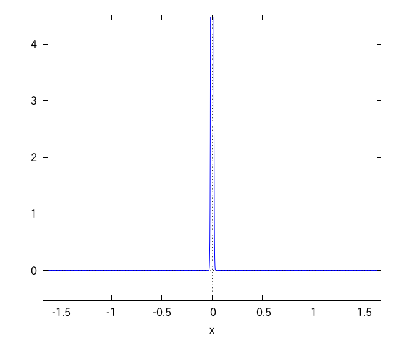
\includegraphics[keepaspectratio, width=6.5cm,height=6cm,clip]{Dirac_Delta_function3.pdf}
                        \caption{ディラックの $\delta$ 関数(1次元)の形}
                        \label{fig:delta_f2}
                    \end{center}
                \end{figure}

                        作り方は簡単.まず,面積1のグラフを用意する(図\ref{fig:delta_f24}).
                \begin{figure}[hbt]
                    \begin{center}
                        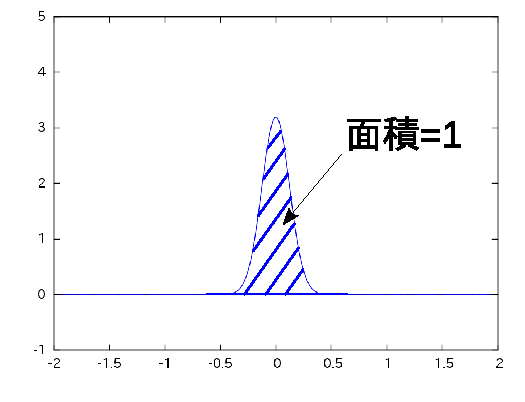
\includegraphics[keepaspectratio, width=6.5cm,height=6cm,clip]{Dirac_Delta_function5.pdf}
                        \caption{ディラックの $\delta$ 関数の作り方1}
                        \label{fig:delta_f24}
                    \end{center}
                \end{figure}

                        そして,面積1を保ちながら無限に細くしていく(図\ref{fig:delta_f33}).
                \begin{figure}[hbt]
                    \begin{center}
                        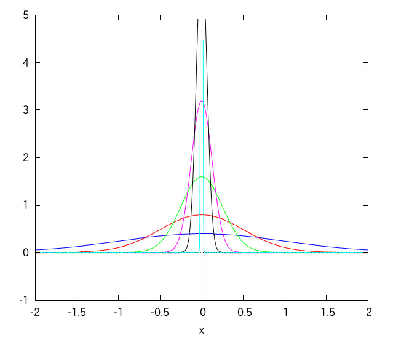
\includegraphics[keepaspectratio, width=6.5cm,height=6cm,clip]{Dirac_Delta_function4.pdf}
                        \caption{ディラックの $\delta$ 関数の作り方2}
                        \label{fig:delta_f33}
                    \end{center}
                \end{figure}
                        これで,面積が1で関数値が無限になる関数を作ることができた.

            $\delta$ 関数には次元があり,[$x^{-1}$] である.次元を持っていることを忘れやすいので,要注意.

                        ついでに,2次元の $\delta$ 関数のグラフも書いておこう.は図\ref{fig:delta_f66}下の通り.
                \begin{figure}[hbt]
                    \begin{center}
                        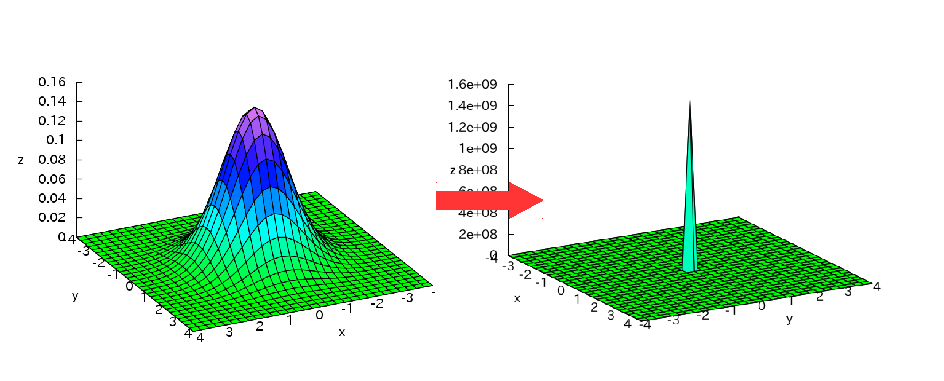
\includegraphics[keepaspectratio, width=6.5cm,height=6cm,clip]{Dirac_Delta_function6.pdf}
                        \caption{ディラックの $\delta$ 関数(2次元)の形}
                        \label{fig:delta_f66}
                    \end{center}
                \end{figure}

                        残念ながら,現実世界である3次元の $\delta$ 関数は図には描けない...

%======================================================================
%  Section
%======================================================================
\section{電流}
%======================================================================
%  SubSection
%======================================================================
    \subsection{電流のイメージ}
    おそらく,電流は説明するまでもないだろう.電気の流れのことである.い
    ままでの言葉を使えば,\textbf{電流} とは電荷の運動のことである,とい
    えよう.観測者Aに対して,荷電粒子が速度を持って運動しているとき,観測
    者Aは荷電粒子を見て,「電流が生じている」と認識するのである.この運動
    する荷電粒子は,一般に,数え切れないほど多くの数であることを想定する
    場合が多い.特に断りのない限り,電流とは,多数の荷電粒子の運動である.

    電気回路に流れる電流も多数の荷電粒子の流れであるが,この荷電粒子は導
    線中を移動することしかできない.そこでここでは,もう少し電流のイメー
    ジを拡張して,任意の空間に流れる電流を認めよう.荷電粒子は導線内部に
    しか存在できないわけではない.真空中に存在することもある.電流は導線
    だけに流れるものではない.

    電流を記号で表すときには,$I$ を用いることが多い.

    電気回路での電流のイメージは図\ref{fig:EM_Denryu01}(A)のようになろう.
    導線の中の電子をイメージしたら,図\ref{fig:EM_Denryu01}(B)の様になるかもしれない.
    しかし,実は図\ref{fig:EM_Denryu01}(B)のイメージは物性物理学的に間違っている.
    実際の電流の発生機構を説明するには原子の構造の解明や量子力学の知識が必要であり,
    それをここで考えることはできない.
    しかし,電磁気学では電荷の流れ方がどのようになっているかは説明できない.
    それとは関係なしに理論が成立している.

    電磁気学での電流とは電荷の移動であり,その場所は問われていない(導線内部である必要はない).
        具体的イメージも大事だが,ここではそれにとらわれず,抽象的な電流を考えるべきである.
        何度も言うが,電流とは空間中を移動する電荷のことである.どのように移動するかは別問題である.
        そうした抽象的な電流を考えるならば,図\ref{fig:EM_Denryu01}(B)のイメージは,
        荷電粒子の通り道を任意の空間と捉えることで,正しいイメージとなる.
        \begin{figure}[hbt]
            \begin{tabular}{cc}
                \begin{minipage}{0.5\hsize}
                    \begin{center}
                        \includegraphicsdouble{EM_Denryu01.pdf}

                        (A) 電気回路
                    \end{center}
                \end{minipage}
                \begin{minipage}{0.5\hsize}
                    \begin{center}
                        \includegraphicsdouble{EM_Denryu02.pdf}

                        (B) 一般化
                    \end{center}
                \end{minipage}
            \end{tabular}
            \caption{電流(イメージ)}
            \label{fig:EM_Denryu01}
        \end{figure}



%======================================================================
%  SubSection
%======================================================================
    \subsection{電流の定義(仮)}
        電流を数式を用いて定義しておこう.電流とは多数の点電荷の集まりの平均的な移動
        のことである.この移動を畏まった言い方をすると,次のように言える.

        ここに電流の通り道(導線)があるとしよう.
        このとき,電流を次のように定義する.
        \\
        \begin{itembox}[l]{\textbf{電流の定義(仮)}}
            \begin{itemize}
                \item 電流とは,導線の断面を単位時間1[s]に通過する
                      電荷の量を,\textbf{電流} という
                \item 電流の単位は[A]という記号で表される
                \item 電荷の単位はクーロン([C])であるので,電流の単位[A]は
                      [A]$=$[C/s]という関係がある
                \item 電流を表す標準的な記号として,このノートでは,$I$,
                      もしくは,$i$ を用いることにする
                        \footnote{
                            記号 $i$ は数学では虚数単位として用いられる
                            記号であるが,物理学や工学では電流を表すことに
                            用いることが多い(その方が一般的).なので,
                            物理学では虚数単位として,$j$ が採用されている.
                            $i$ の次のアルファベットだからだろうか.おそらく,
                            特別の意味などはないはず.文字の意味に注意しよう.
                        }
            \end{itemize}
        \end{itembox}
        \\
        \begin{figure}[hbt]
            \begin{center}
                \includegraphicslarge{EM_Denryu.pdf}
                \caption{電流(イメージ)}
                \label{fig:EM_Denryu}
            \end{center}
        \end{figure}

    \begin{memo}{注意}
        実は,この電流の単位は現在では採用されていない.
        正式な単位の定義は,後に必要な知識を説明した上で行う.
        電流に単位がないと,電流に関する事柄を扱いにくいので,
        ここではとりあえず,最も直感的で自然な定義を説明した.
        この節で「(仮)」と表現しているのは,このことによる.
    \end{memo}

%======================================================================
%  SubSection
%======================================================================
    \subsection{電流密度}
    電流とは,導線の垂直断面を,一秒間に流れる電気量として定義した.
    さらにここで,単位断面積1[m${}^{2}$]を単位時間1[s]の間に,
    どのくらいの電流が生じるかを示す \textbf{電流密度} を定義する
        \footnote{
            注意しておこう.電流密度の“密度”とは,単位面積当たりの
            密度のことである.電荷密度では,単位体積当たりの密度のこ
            とであり,両者(電荷密度と電流密度)の“密度”という語彙
            の違いは区別しておく必要がある.(次元解析をしていて,これ
            らの単位を混同してしまって,頭が混乱してしまったことがあ
            る.時間の無駄であった.)
        }.

        導線に生じている電流 $I$ が,いかなる場合でも,一様で
            \footnote{
                一様に:“むらなく”とか,“偏りなく”といった意味で使用される語彙.
            }
        あるならば,電流密度を導入することは無駄である.しかし,
        現実には,導線に生じる電流は一様ではなく,ある部分に集中的に多く
        流れていたり,ある部分には電荷の流れが全くないこともある.たしかに
        導線全体を見渡した正味の電流は一定値をとっているが,その導線の内部
        を詳細に見ることができるならば,電流にむらがあることを知るだろう.

        電流密度を $\bi(\br)$ と表す.単位は[A/m${}^{2}$]である
            \footnote{
                電荷密度 $\rho$ の単位 [C/m${}^{3}$]との違いに注意.
                電流密度は単位面積当たりの量で,電荷密度は単位体積当たり
                の量である.
            }.
        \begin{figure}[hbt]
            \begin{center}
                \includegraphicslarge{EM_DenryuMitsudo1.pdf}
                \caption{電流密度(イメージ)}
                \label{fig:EM_DenryuMitsudo1}
            \end{center}
        \end{figure}

%======================================================================
%  SubSection
%======================================================================
    \subsection{電流密度と電流の関係}
        電流 $\bI$ と電流密度 $\bi$ の関係を示そう.
        まず,電流の大きさ $I=|\bI|$ と電流密度 $\bi(\br)$ の関係を考える.

        導線の断面を $S_{l}$ とし,また,
        その一部の微小断面を $\df S_{l}$ とする
            \footnote{
                添字の $l$ は曲面 $S_{l}$ の縁となる閉曲線を表す.
                一般に,曲面は縁があるはずで,その縁は閉曲線である.
            }.
        この微小断面 $\df S_{l}$ の単位法線ベクトルを $\bn(\br)$ とかこう.

        このとき,電流密度 $\bi(\br)$ の微小断面 $\df S_{l}$ の垂直成分は
            \begin{align*}
                \bi(\br) \cdot \bn(\br) \df S_{l}
            \end{align*}
        で表現できる.そして,これを全断面 $S$ で面積分した値は,
        電流の大きさ $I$ に等しい.すなわち,
            \begin{align*}
                I = \sint_{S_{l}}\bi(\br) \cdot \bn(\br) \df S_{l}.
            \end{align*}

        まとめておこう.
        \begin{myshadebox}{電流密度と電流の関係}
            閉曲線 $l$ を縁とする曲面 $S_{l}$ を貫く電流 $I$ と,
            電流密度 $\bi(\br)$ の関係は,次式で表される.
            \begin{align}
                I = \sint_{S_{l}}\bi(\br) \cdot \bn(\br) \df S_{l}.
            \end{align}
            ここに,$\bn(\br)$ は $S_{l}$における各微小部分 $\df S_{l}$ の
            単位法線ベクトルである.
        \end{myshadebox}

        \begin{figure}[hbt]
            \begin{center}
                \includegraphicslarge{LI_si_00.pdf}
                \caption{電流と電流密度}
                \label{fig:LI_si_00}
            \end{center}
        \end{figure}

    \begin{memo}{微小面積と単位法線ベクトル}
        微小面積とは,全面積 $S$ の微小な一部分のことである.
        また,単位法線ベクトルとは,面に垂直方向で長さが1のベクトルのことである.
        \begin{figure}[hbt]
            \begin{center}
                \includegraphicslarge{EM_smollS.pdf}
                \caption{微小体積}
                \label{fig:EM_smollS}
            \end{center}
        \end{figure}
    \end{memo}

    \begin{memo}{面積分の表示方法}
        面積分は,2方向にわたる積分である.
        つまり,2つの積分変数 $u$,$v$ を
        考えたとき,これを変数に持つ関数 $f(u,\,v)$ をとし,
            \begin{align*}
                \int \left( \int f(u,\,v) \df u \right) \df v
            \end{align*}
        を計算することが,面積分を行うということである.

        つまり,$f(u,\,v)$ を最初に $u$ について積分して,その結果をさらに,
        $v$ について積分するということである.計算方法を示すには,このような
        表示の仕方が有効であるが,この表現からでは面積分であることをイメージする
        には,少々難しい.そこで,式を次ように書き換えてみる.
            \begin{align*}
                 \sint f(u,\,v) \df u \df v
            \end{align*}
        括弧をなくしただけである.そして,
        $\df S := \df u\df v$ という量を導入し,
        さらに,2回の積分を改て $\sint_{S}$ と表現することで,
            \begin{align*}
                \sint_{S} f(u,\,v) \df S
            \end{align*}
        となる.これならば,面 $S$ で面積分するというイメージが
        しやすい式の表現になった.

        ちなみに,$\df S := \df u\df v$ は \textbf{面積素} とよばれる.
    \end{memo}



%   %-----------------------------------------------------------------------------------------------
%   %  Input
%   %    File Name : PhysNote_EM_1st_RShipIandRho.tex
%   %    説明      : 電流と電荷の関係を説明する.
%   %-----------------------------------------------------------------------------------------------
        %===================================================================================================
%  Chapter : 電磁気学の基本概念
%  説明    : 電荷の存在や,電流の存在などを確認する
%===================================================================================================
%======================================================================
%  Section
%======================================================================
\section{電流と電荷の関係}
\begin{mycomment}
    \textbf{電荷} とは,電磁気現象の発生原因であり,この存在は有無をいわさず
    受け入れさせられるものである.\textbf{電流} とは,一つ,あるいは複数(多数)の
    電荷が,平均的に一方向に移動しているような現象をいう.従って,
    電流とは,電荷と観測者の相対的な速度に依存していると考えられる.つまり,
    観測者が電荷を見ているとき,その観測者の速度により,電流が生じているのか,
    単に電荷が運動せずにその場に存在しているのかが,変わってきてしまう.
    そこで,以降では,観測者の速度を0として,扱うことにする.
\end{mycomment}
%======================================================================
%  SubSection
%======================================================================
    \subsection{大局的な電荷保存則}
        \begin{mysmallsec}{電荷は突然現れることはない}
        ある領域に電荷が多数存在していることを想定しよう(図\ref{fig:Denryu_Denka_intoro}(A)参照).
        この多数の電荷の電気量の総和を,$Q(t)$ と書くことにする
            \footnote{
                電荷が多数存在するが,その個数は有限であることを想定する.
                このとき,電荷に番号付けをして,$q_{0}$,$q_{1}$,$q_{2}$,$\cdots$ の
                ように書けば,その総和 $Q(t)$ は $Q(t):=\sum_{i}^{N(t)}q_{i}$ で表せる.
                左辺の総電気量 $Q(t)$ の独立変数 $t$ は,右辺の電荷の個数が時間変化する場合($N(t)$)を
                表したものである.
            }.
        この状態から,ある程度時間が経過して,領域内部の電気量の総和が変化したとしよう.
        つまり,$Q$ の時間微分が0ではない値をとるということになる
            \footnote{
                時間変化がないということは,時間微分して0であるということである.
                例えば,速さ $v(t)$ は $v(t):=\df x(t)/\df t$($x$ は位置,$t$ は時間を表す)で
                定義されるが,位置に時間変化がない場合 $x(t)$ は一点に止まっているので,
                $x(t)=X_{\mathrm{const}}$ となり,時間によらない定数 $X_{\mathrm{const}}$ で表せる.
                この時の速度を考えると,$v(t):=\df x(t)/\df t=\df X_{\mathrm{const}}/\df t = 0$ と
                なり,位置の時間微分は0である.つまり,位置が時間変化しない(動かない)物体の
                一の時間微分は0になる.これは逆に,位置の時間微分が0であれば,
                その物体は動いていない,と言うこともできる.さらに,物体の位置の時間微分が0でない値
                を取るならば,その物体は動いていると言える.

                今回の場合,時間変化するのは領域内の総電気量 $Q(t)$ である.
            }.
        総電気量が変化したということは,その領域内部の電荷の量が変化したということである.
        つまり,個々の電荷が領域外部に出て行ったり,あるいは逆に,領域外部から電荷が入ってきた
        ということである.すなわち,
            \begin{equation*}
                \frac{\df Q(t)}{\df t} \neq 0.
            \end{equation*}
        ここで,出たり入ったりする電荷の,正味の電気量を $I(t)$ と書けば,
            \footnote{
                ここで記号として $I(t)$ を書いたのは,電流 $I(t)$をあとで定義する
                ためである.独立変数として,時間 $t$ を明示したのは,時刻によって
                生じる電流が,異なる場合を想定したからである.
            },
            \begin{equation*}
                \frac{\df Q(t)}{\df t} + I(t) = 0.
            \end{equation*}
        となるような $I(t)$ が存在することになる.要は,領域内部の総電気量 $Q(t)$ の
        時間変化に,正味の電荷の出入り $I(t)$ を足し合わせれば0であるということである.
        もっと簡単に言うと,領域内部の総電気量の変化は,外部との電荷のやり取りで
        生じるのであり,その領域内部でいきなり電荷が現れたり消えたりしない,という
        ことである(図\ref{fig:Denryu_Denka_intoro}(B)参照).この電荷の出入りを表す $I(t)$ が
        電流である.端的に言えば,ある領域内の総電気量が変化したことと,その領域に電流が生じ
        ていることとは,等価である.
        \end{mysmallsec}

        \begin{mysmallsec}{電荷保存の法則}
        実は,この考え方こそが,\textbf{電荷保存の法則} であり
            \footnote{
                略して,\textbf{電荷保存則} といわれることのほうが,一般的である.
            },今の場合は,
        \textbf{大域的(マクロ)な}視点から見た電荷保存則(脚注参照)である.後ほど,一般化して,
        \textbf{局所的な}電荷保存則も紹介することになる.

        改めて,大局的な電荷保存則を記述しておこう.
            \begin{myshadebox}{(大局的な)電荷保存則}
                ある領域内部の総電気量を $Q(t)$ とし,その内部から外部へ向かって電流 $I(t)$ が
                生じている場合,
                \begin{align}
                    \frac{\df Q(t)}{\df t} = - I(t).
                \end{align}
                という関係式が成立する.これを,
                大局的な \textbf{電荷保存の法則}(あるいは略して,\textbf{電荷保存則})という.
            \end{myshadebox}

        ここで,電流 $I(t)$ を右辺に移項した.この表現の方が,総電気量の時間変化と
        電流が等価であることを,イメージしやすいからである.また,多くの教科書で,
        この書き方がなされている.電流の符号は,領域内の総電気量が減る場合には正
        (電荷が領域内部から飛び出して,それが電流となる),
        領域内の総電気量が増える場合には負(領域内に電流が入ってきて,内部の電荷個数が増える)とする
            \footnote{
                簡単に言うと,領域から電流が外向きに生じているときに正,
                領域に電流が吸収される場合に負とする.
            }.
        \end{mysmallsec}
                \begin{figure}[hbt]
                    \begin{tabular}{cc}
                        \begin{minipage}{0.5\hsize}
                            \begin{center}
                                \includegraphicsdouble{Denryu_Denka_intoro001.pdf}

                                (A) 領域内の電荷
                            \end{center}
                        \end{minipage}
                        \begin{minipage}{0.5\hsize}
                            \begin{center}
                                \includegraphicsdouble{Denryu_Denka_intoro002.pdf}

                                (B) 電荷の出入り
                            \end{center}
                        \end{minipage}
                    \end{tabular}
                        \caption{電流と電荷}
                        \label{fig:Denryu_Denka_intoro}
                \end{figure}

%======================================================================
%  SubSection
%======================================================================
    \subsection{局所的な電荷保存則}
        電荷保存則は,局所的にも成立する法則である.理論物理学では,
        大局的表現よりも,これから説明する局所的な電荷保存則の表現
        がよく使われる.大局的な表現がすでに得られているので,そこ
        から,局所的表現を導出しよう.

        まず,電流 $I(t)$ と総電気量 $Q(t)$ を,それぞれ電流密度 $\bi$ と
        電荷密度 $\rho$ で書きなおしておこう.
            \begin{align*}
                I(t)  &=  \sint_{S} \bi \cdot \bn \df S. \\
                Q(t)  &=  \vint_{\Omega_{S}} \rho \df V.
            \end{align*}
        電流道度 $\bi$ と電荷密度 $\rho$ は,位置と時間の関数であることに注意.
            \begin{equation*}
                \bi := \bi(\br,\,t)\,,\quad \rho := \rho(\br,\,t).
            \end{equation*}
        ちなみに,電流 $I(t)$ と総電気量 $Q(t)$ の独立変数に位置 $\br$ が
        ないのは,位置で積分してしまうためである
            \footnote{
                積分変数は積分後には残らない.大局的視点から見るので,
                細かな位置を知る必要はなく,この視点で重要なのは,考察範囲
                全体の電流量や電気量なのである.これから考える局所的な量は,
                その位置も重要になる.大局的視点と局所的視点の違いは意識して
                おくべきことだろう.
            }.
        電流道度 $\bi$ と電荷密度 $\rho$ を用いると,電荷保存則は次のように書ける.
            \begin{equation*}
                 \frac{\rd}{\rd t} \left( \vint_{\Omega_{S}} \rho \df V \right)
               = - \sint_{S} \bi \cdot \bn \df S.
            \end{equation*}

        ここで,上式の右辺にガウスの定理
            \footnote{
                任意のベクトル $\bX$ に対して,
                \begin{equation*}
                      \sint_{S} \bX \cdot \bn \df S
                    = \vint_{\Omega_{S}} \ddiv \bX \cdot \bn \df V.
                \end{equation*}

                後で簡単に復習するので,そこを参照のこと.
                それでもわからなければ,数学の解説の部分を
                読むこと.さらにそれでもわからなかったら,
                ベクトル解析教科書を別途お読みください.
            }
        を適用する.
            \begin{equation*}
                  \vint_{\Omega_{S}} \frac{\rd \rho}{\rd t} \df V
                = - \vint_{\Omega_{S}} \ddiv \bi \cdot \bn \df V.
            \end{equation*}
        この式変形で,左辺の空間微分と時間微分の可換性
            \footnote{
                空間に関する微分と,時間に関する微分は計算順序を入れ替えても,
                結果は変わらないということ.
            }
        を利用した.
        この式の両辺を見ると,積分範囲が同じ体積分になっている.この等式が一般的に成り立つのは,
        両辺の被積分関数が等しいときである
            \footnote{
                数学的に示すべきことだろうが,ここでは割愛する.
            }.
            \begin{equation*}
                  \frac{\rd \rho}{\rd t} = -\ddiv \bi.
            \end{equation*}
        慣習に従って,次のように書き換える.
            \begin{align}\label{eq:bisiteki_denkahozonsoku00}
                \ddiv \bi = -\frac{\rd \rho}{\rd t}.
            \end{align}
        この式(\ref{eq:bisiteki_denkahozonsoku00})が,
        局所的な \textbf{電荷保存則} である.

        ある局所的領域
            \footnote{
                局所的領域:可能なかぎり小さくした領域のこと.あくまでも,
                直感的な言葉であり,「可能なかぎり」に特別な意味は込めていない.
                日常言語的な捉え方をしてもらいたい.
            }
        から電流が湧き出る($\ddiv \bi$)ならば,その領域内部の電荷密度は
        減少する($-(\rd \rho/\rd t)$)ということを,式で表現できている.

        改めて,まとめておこう.
            \begin{myshadebox}{(局所的な)電荷保存則}
                ある局所的領域から電流が湧き出る($\ddiv \bi$)ならば,
                その領域内部の電荷密度は減少する($-\rd \rho/\rd t$).
                \begin{align}
                    \ddiv \bi = -\frac{\rd \rho}{\rd t}.
                \end{align}
                これは,電荷保存則を局所的に表現したものである.
            \end{myshadebox}

            \begin{memo}{ガウスの定理(復習)}
                ガウスの定理:ガウスの法則とは別のもの.ガウスの定理は数学上の
                              定理である.この定理により,以下の等式が成立する.

                                任意のベクトル $\bX$ に対して,
                                \begin{equation*}
                                      \sint_{S} \bX \cdot \bn \df S
                                    = \vint_{\Omega_{S}} \ddiv \bX \cdot \bn \df V.
                                \end{equation*}

                                言葉で説明するならば,次のようなイメージになろう.
                                「任意の閉曲面 $S$ で囲まれた領域 $\Omega_{S}$ より
                                湧き出る $\ddiv \bX$ の総和は,閉曲面 $S$ の表面から
                                抜け出る正味の流出量に等しい」.
            \end{memo}



%===================================================================================================
%  Chapter : クーロンの法則
%  説明    : 電磁気学の要である,電気力=クーロン力について説明する
%===================================================================================================
\chapter{クーロンの法則}
%   %-----------------------------------------------------------------------------------------------
%   %  Input
%   %    File Name : PhysNote_EM_1st_CoulombLow.tex
%   %    説明      : 電場を導入する
%   %                を説明する.
%   %-----------------------------------------------------------------------------------------------
        %===================================================================================================
%  Chapter : クーロンの法則
%  説明    : 電磁気学の要である,電気力=クーロン力について説明する
%===================================================================================================
%======================================================================
%  Section
%======================================================================
    \section{クーロン力}\label{sec:CoulomnbForce}
%   %==================================================================
%   %  Subsection
%   %==================================================================
    \subsection{法則}
        電荷を帯びた物体が受ける,電気的な力というものが,世の中に
        存在する.これは万人が知っている事実だから,ここで改めて明
        記することは,バカバカしく感じられる.しかし,この電気的な
        力の存在は,大変重要なものである.この電気的な力のことを,
        \textbf{クーロン力} とよぶ.電気量の単位であるクーロンと同
        じ名前を持っているが,お察しのとおり,同一人物に由来するも
        のである.

        クーロン(Coulomb)は,電気的な力の性質を実験的に知ることに
        成功した
            \footnote{
                電気量の定義は,クーロン力を基にしてなされるもの
                である.
            }.
        そして,クーロンは,電気的な力が,次のような性質を持っていることを
        明らかにした.
        \\
        \begin{itembox}[l]{\textbf{クーロン力(クーロンの法則)}}
            ここに,電荷が2つあるとしよう.この2つの電荷は区別する
            ことができて,$q_{1}$,$q_{2}$ という電気量を持っている
            とする.電荷 $q_{1}$ と $q_{2}$ との距離を $r$ としたと
            き,この2つの電荷が受ける力は,以下のような規則がある.
            \begin{itemize}
                \item 2つの電荷の電気量が互いに異なる符号をもってい
                      るならば,両電荷は互いに引き合う向きに力を受
                      ける
                \item 2つの電荷の電気量が同じ符号を持っているならば,
                      両電荷は互いに反発しあう向きに力を受ける.
                \item 2つの電荷の受ける力の大きさは等しく,
                      向きは互いに逆向きである
                \item 2つの電荷が受ける力の大きさは,
                      2つの電荷の電気量の積($q_{1}q_{2}$)に比例する.
                \item 2つの電荷が受ける力の大きさは,
                      2つの電荷間の距離の2乗($r^{2}$)に反比例する.
            \end{itemize}
        \end{itembox}
        \\
        \begin{figure}[hbt]
            \begin{tabular}{cc}
                \begin{minipage}{0.5\hsize}
                    \begin{center}
                        \includegraphicsdouble{coulombs_low1.pdf}

                        (A)
                    \end{center}
                \end{minipage}
                \begin{minipage}{0.5\hsize}
                    \begin{center}
                        \includegraphicsdouble{coulombs_low2.pdf}

                        (B)
                    \end{center}
                \end{minipage}
            \end{tabular}
                        \caption{クーロン力}
                        \label{fig:coulombs_low}
        \end{figure}

        上に書いたような,クーロン力が示す性質のことを,\textbf{クーロンの法則} と
        いう.これは電磁気学の最も基本的な法則であり,大変重要な法則である.
        あとに説明する \textbf{電場} という重要な概念の導入も,
        このクーロンの法則を基にしている.

        言葉で書いてしまうと,ちょっとややこしいかもしれない.
        しかし,いきなり数式を出してしまうと,それはそれで
        尻込みしてしまうので,とりあえず言葉で説明してみた.

%   %==================================================================
%   %  Subsection
%   %==================================================================
    \subsection{定量化}
        では,次の段階に進み,クーロンの法則を数式で表現してみよう.
        数式で表現すると,とても簡潔になることを感じ取ることができる
        だろう.

        図\ref{fig:Coulombs_Force}のような状態であるとしよう.
        \begin{figure}[hbt]
            \begin{center}
                \includegraphicslarge{Coulombs_Force.pdf}
                \caption{クーロンの法則}
                \label{fig:Coulombs_Force}
            \end{center}
        \end{figure}

        2つの区別可能な電荷が存在し,それぞれの電気量が,$q_{1}$,$q_{2}$ で
        あるとする.また今後,これらの電荷自体を表現する場合にも,
        「電荷 $q_{1}$」などのように記述する
            \footnote{
                同じ記号に二つの意味を込めるのはよくないが,
                そうかと言って,無嫌味に記号を増やして読みづらくしたくも
                ない.ここでは,誤解を生むことがないと判断し,同じ記号で
                “電荷それ自体”と“その電気量”の2つを同じ記号で表すこと
                とする.
            }.
        この2つの電荷がある位置を,それぞれ $\br_{1}$,$\br_{2}$ と
        する.このとき,電荷間の距離 $r$ は,
            \begin{equation*}
                r = | \br_{2} - \br_{1} |.
            \end{equation*}
        また,電荷 $q_{2}$ から見た,電荷 $q_{1}$ の位置 $\br_{12}$は,
            \begin{equation*}
                \br_{12} = \br_{1} - \br_{2}.
            \end{equation*}
        同様に,電荷 $q_{1}$ から見た,電荷 $q_{2}$ の位置 $\br_{21}$は,
            \begin{equation*}
                \br_{21} = \br_{2} - \br_{1}.
            \end{equation*}

        「2つの電荷が受ける力は,大きさが同じで,向きが逆である.」これを
        数式で表すには,まず,大きさと向きを文字で表現すべきだ.
        同時に考えるのは難しいので,まずはクーロン力の大きさだけを考える.
        電荷 $q_{1}$ が受けるクーロン力 $F_{12}$ は,
        2点電荷の電気量の積 $q_{1}q_{2}$ に比例するので,数式的には,
            \begin{equation*}
                F_{12} = \alpha q_{1}q_{2}
            \end{equation*}
        とかける.ここに,$\alpha$ 比例定数である
            \footnote{
                この比例定数 $\alpha$ には全く意味が無い.単に
                比例を表すのに,便宜的に使ったに過ぎない.
                同じことがすぐ後に使う,$\beta$ についても言える.
                しかし,最後に現れる比例定数 $k$ については,
                重要であるので注意すべきだ.
            }.
         また同時に,
        「2つの電荷が受ける力の大きさは,2つの電荷間の距離の
        2乗($r^{2}$)に反比例する」から,
            \begin{equation*}
                F_{12} = \beta \frac{1}{r^{2}}
            \end{equation*}
        ともかける.$\beta$ も比例定数である.
        この2つの $F_{12}$ の式は矛盾なく両立する.
        この2つの式をまとめて,
            \begin{equation*}
                F_{12} = \alpha \beta \frac{q_{1}q_{2}}{r^{2}}
            \end{equation*}
        となる.ここで,式の見易さのため,比例定数 $\alpha \beta$ を
        改めて $k$ とおいて($k=\alpha \beta$),
            \begin{align}\label{eq:coulomb_force_f1_ookisa}
                F_{12} = k \frac{q_{1}q_{2}}{r^{2}}
            \end{align}
        とすれば,この式(\ref{eq:coulomb_force_f1_ookisa})によって,
        電荷 $q_{1}$ が受けるクーロン力の大きさを
        記述できたことになる.

        残りはその方向であるが,これは簡単だ.単位ベクトルを考えれば
        よい.一般のベクトル $\bA$ に対する単位ベクトルとは,大きさが $1$ で,
        その方向が $\bA$ と同じ向きのようなものである.このような単位ベクトルが
        存在したとして,$\bn$ と表そう.この時,$\bA$ は,$\bA=|\bA|\bn$ と書き
        表せる.つまり,単位ベクトル $\bn$ について解けば,
            \begin{equation*}
                \bn = \frac{\bA}{|\bA|}
            \end{equation*}
        である.

        今の場合に当てはめて考えれば,$\bA=\br_{12}$ であるから,
        単位ベクトルは
            \begin{equation*}
                \bn = \frac{\br_{12}}{|\br_{12}|}
                    = \frac{\br_{1} - \br_{2}}{|\br_{1} - \br_{2}|}
            \end{equation*}
        である.これが,電荷 $q_{1}$ が受けるクーロン力の向きを
        表している.

        これで,電荷 $q_{1}$ の受けるクーロン力の大きさと向きの
        数式的表現を,別々ではあるが,表現できた.あとは
        この2つを一緒に表せれば,完了となる.

        ここで改めて,電荷 $q_{1}$ の受ける
        クーロン力を向きも考慮して $\bF_{12}$ と表すこととすると,
        $\bF_{12}$ は,その大きさ $F_{12}$ と単位ベクトル $\bn$ を
        用いて,
            \begin{equation*}
                \bF_{12} = F_{1}\bn
            \end{equation*}
        とかける.
        これに,上で得た結果を代入すればよい.すると,
            \begin{align}\label{eq:coulomb_force_f1}
                \bF_{12} = k \frac{q_{1}q_{2}}{r^{2}} \frac{\br_{1} - \br_{2}}{|\br_{1} - \br_{2}|}
            \end{align}
        となる.この式(\ref{eq:coulomb_force_f1})が目標としていた,
        電荷 $q_{1}$ が受けるクーロン力 $\bF_{12}$を,
        式で表したものである.

        これ同様に,電荷 $q_{2}$ が受けるクーロン力 $\bF_{2}$を考えること
        ができるが,「2つの電荷の受ける力の大きさは等しく,向きは互いに逆
        向きである」ということを考慮すれば,直ちに,次式を得る.
            \begin{align*}
                \bF_{21} &= - \bF_{12} \\
                        &= - k \frac{q_{1}q_{2}}{r^{2}} \frac{\br_{1} - \br_{2}}{|\br_{1} - \br_{2}|}.
            \end{align*}
        ここで,
            \begin{align*}
                -(\br_{1} - \br_{2}) &= \br_{2} - \br_{1} \\
                |\br_{1} - \br_{2}|  &= |\br_{2} - \br_{1}| \\
                q_{1}q_{2}           &= q_{2}q_{1}
            \end{align*}
        であることに気付けば
            \footnote{
                数式を見れば当たり前のように感じるかもしれないが,重要な式である.というのも,
                この関係式は作用反作用の法則を表す数式にほかならないからである.
            },
            \begin{align}\label{eq:coulomb_force_f2}
                \bF_{21} = k \frac{q_{2}q_{1}}{r^{2}} \frac{\br_{2} - \br_{1}}{|\br_{2} - \br_{1}|}
            \end{align}
        となる.$\bF_{12}$ の式(\ref{eq:coulomb_force_f1}) と比較すると,
        添字の1と2が逆になっているだけであることに気づくだろう.

        最後に,比例定数 $k$ について記述しよう.
        この比例定数は,基準とする単位系によって値は
        変化するが,今日一般的に使用されているSI単位系を
        採用するならば,
            \begin{align}
                k = \frac{1}{4\pi\varepsilon_{0}} = 8.989 \times 10^{9}
            \end{align}
        である.$\varepsilon_{0}$ は真空の \textbf{誘電率} と言われる
        物理定数であるが,これについての解説は後回しにする.
        また,$\pi$ は円周率である.

%   %==================================================================
%   %  Subsection
%   %==================================================================
    \subsection{まとめ}
        以上の計算より得た結果をまとめよう.
        \begin{myshadebox}{クーロン力}
            ある空間に2つの電荷 $q_{1}$,$q_{2}$ が,それぞれ
            位置 $\br_{1}$,$\br_{2}$ に
            存在するとき,この2つの電荷には,次式で
            表されるような力が作用する.この力のこと
            を \textbf{クーロン力} という.

            電荷 $q_{1}$ に対して働く力は以下.
               \begin{align}
                   \bF_{12} =
                       \frac{1}{4\pi\varepsilon_{0}} \frac{q_{1}q_{2}}{r^{2}}
                           \frac{\br_{1} - \br_{2}}{|\br_{1} - \br_{2}|}.
               \end{align}

        ここに,$\varepsilon_{0}$ は真空の誘電率
           \footnote{
               詳細は後述.
           }
        である.
        \end{myshadebox}


        電荷 $q_{2}$ に対しては,以下の力が働く.
           \begin{align}
               \bF_{12} = -\bF_{21} =
                   \frac{1}{4\pi\varepsilon_{0}} \frac{q_{2}q_{1}}{r^{2}}
                       \frac{\br_{2} - \br_{1}}{|\br_{2} - \br_{1}|}.
           \end{align}


    \begin{memo}{(例)2つの点電荷同士のクーロン力}
    クーロンの法則を,より感覚的に分かるように,ここで,
    最も簡単な,2つの点電荷間に働く,クーロン力を考てみよう.

    存在する電荷が点電荷の場合,クーロンの法則は次式で表せる.
            \begin{align}
                \bF_{12}=\frac{1}{4\pi\varepsilon_{0}}
                \frac{q_{1}q_{2}}{|\br_{1}-\br_{2}|^{2}}
                \frac{\br_{1}-\br_{2}}
                     {|\br_{1}-\br_{2}|}.
            \end{align}
    より考えやすくするために,2次元で考えてみよう.座標系は,直交座標系とする.
    この場合,
        \begin{equation*}
            |\br_{1}-\br_{2}| = \sqrt{ {\left(x_{2} - x_{1}\right)}^{2}
            + {\left(y_{2} - y_{1}\right)}^{2} }
        \end{equation*}
    である.
        \begin{figure}[hbt]
            \begin{center}
                \includegraphicslarge{2point_distance.pdf}
                \caption{一般の2つの点の間の距離}
                \label{fig:2point_distance}
            \end{center}
        \end{figure}


    点電荷の配置を,$x$ 軸上にし,各電荷が $x=-1/2$,$x=1/2$ に存在しているとする.
    そうすると,2つの点電荷のそれぞれの位置ベクトルは,
    $\br_{1}  =  ( \,-1/2\,,\,0\, )$,$\br_{2}  =  ( \,1/2\,,\,0\, )$ となる.
    そうすると,
            \begin{align*}
                |\br_{1}-\br_{2}|
                &= \sqrt{ {\left(x_{2} - x_{1}\right)}^{2} + {\left(y_{2} - y_{1}\right)}^{2} } \\
                &= \sqrt{ {\left(\frac{1}{2} - \left(-\frac{1}{2}\right)\right)}^{2} + {\left(0-0\right)}^{2} } \\
                &= 1.
            \end{align*}
    電荷量の
    大きさは,両電荷ともに等しく,$1$[C] として考える.
        \begin{figure}[hbt]
            \begin{center}
                \includegraphicslarge{example_Coulombs_low1.pdf}
                \caption{例:2つの点電荷間のクーロン力}
                \label{fig:example_Coulombs_low1}
            \end{center}
        \end{figure}

    すると,クーロンの法則は,次のようになる.電荷 $q_{1}$ が,電荷 $q_{2}$ から
    受けるクーロン力 $\bF_{12}$ は
            \begin{align*}
                \bF_{12}
                &= \frac{1}{4\pi\varepsilon_{0}}
                \frac{q_{1}q_{2}}{|\br_{1}-\br_{2}|^{2}}
                \frac{\br_{1}-\br_{2}}
                     {|\br_{1}-\br_{2}|} \\
                &= \frac{1}{4\pi\varepsilon_{0}}
                \frac{1}{ 1 }
                \frac{\left( \,-1\,,\,0\, \right)}
                     { 1 } \\
                &= \frac{1}{4\pi\varepsilon_{0}} \left( \,-1\,,\,0\, \right)
            \end{align*}
    と書ける.

    クーロン力の向きは,$\left( \,-1\,,0\,\right)$ であることが
    分かった.

    以下では,クーロン力の大きさのみ($| \bF_{12} | := F_{12}$)を考えていこう.
        \begin{align*}
            |\bF_{12}|  &= F_{12} \\
                        &= \frac{1}{4\pi\varepsilon_{0}} \sqrt{(-1)^{2}+0^{2}} \\
                        &= \frac{1}{4\pi\varepsilon_{0}} \cdot 1               \\
                        &= \frac{1}{4\pi\varepsilon_{0}}
        \end{align*}

    最後に,$\varepsilon_{0}$,$\pi$ に具体的な数値を代入する.
    ここではとりあえず,
        \begin{equation*}
            \varepsilon_{0} = 8.854 \times 10^{-12}
        \end{equation*}
    であることが知られているので,この数値を使うことにする.
    しかし,どのようにして,このような数値が分かるかについては,
    後ほど,電磁気学をさらに学んでから,考えなおすことにしたい.
    $\pi$ は周知のように,
        \begin{equation*}
            \pi = 3.141
        \end{equation*}
    である.

    以上から,
            \begin{align*}
                F_{12}
                &= \frac{1}{4\pi\varepsilon_{0}} \\
                &= \frac{1}{4 \times 3.1415 \times 8.854 \times 10^{-12}} \\
                &= \frac{10^{12}}{ 222.483 }  \\
                &= 0.008989 \times 10^{12}  \\
                \therefore\quad
                F_{12}
                &= 8.989 \times 10^{9}
            \end{align*}
    を得る.

    実は,今までの計算は,単位電荷1[C]をもつ2つの点電荷が,1[m]離れて位置する
    場合のクーロン力を計算していた.つまり,
        \begin{equation*}
            \frac{q_{1}q_{2}}{r^{2}} = 1
        \end{equation*}
    となるのは,あたり前のことであった.しかし,
    あえて,座標から丁寧に計算したのは,点電荷がどのような位置に存在しても,
    同じように計算できることを,示したかったからである
        \footnote{
            この例はとても簡単だが,一般性が高い理論であることを認識
            することはできるはず.
        }.

    上の計算から,
        \begin{align}
            \frac{1}{4\varepsilon_{0} \pi} \simeq 9.0 \times 10^{9}
        \end{align}
    が分かる.この数値を用いて,クーロン力を表すと,
        \begin{align}
            F = 9.0 \times 10^{9} \times \frac{q_{1}q_{2}}{r^{2}}
        \end{align}
    となる.

    高校物理では,$k=9.0 \times 10^{9}$ と置いて,
        \begin{equation*}
            F = k \frac{q_{1}q_{2}}{r^{2}}
        \end{equation*}
    と書かれることも多い.
\end{memo}

%======================================================================
%  Section
%======================================================================
    \section{力の重ねあわせの原理}
        クーロン力は,力学的な力と同様に,重ねあわせの原理が成立
        していることが,実験的に確認されている.

        具体例で示したほうが,分かりやすい.
        3つの点電荷が存在する場合を考える.
        \begin{figure}[hbt]
            \begin{center}
                \includegraphicslarge{EM_Coulomb_KasaneAwase01.pdf}
                \caption{クーロン力(3つの点電荷)}
                \label{fig:EM_Coulomb_KasaneAwase00}
            \end{center}
        \end{figure}

        電気量 $q_{1}$,$q_{2}$,$q_{3}$ をもつ3つの点電荷
        の内,任意に2つを選ぶ.ここでは $q_{1}$ と $q_{2}$ をえらぼう.
        ここでは,例として,点電荷 $q_{1}$ が,他の点電荷 $q_{2}$ と $q_{3}$ から受ける
        クーロン力 $\bF_{1}$ を計算する.
        計算方法は,最初に点電荷 $q_{2}$ から受けるクーロン力 $\bldf_{12}$ を
        計算する.この時,$q_{3}$ はとりあえず存在しないとして考える
        (図\ref{fig:EM_Coulomb_KasaneAwase02}(A)).
            \begin{equation*}
                \bldf_{12} = \frac{1}{4\pi\varepsilon_{0}}
                           \frac{q_{2}q_{1}}{{|\br_{1} - \br_{2}|}^{2}}
                           \frac{\br_{1} - \br_{2}}{|\br_{1} - \br_{2}|}.
            \end{equation*}
        その次に,点電荷 $q_{3}$ から受けるクーロン力 $\bldf_{13}$ を
        計算する.この時,$q_{2}$ はとりあえず存在しないとして考える
        (図\ref{fig:EM_Coulomb_KasaneAwase02}(B)).
            \begin{equation*}
                \bldf_{13} = \frac{1}{4\pi\varepsilon_{0}}
                           \frac{q_{3}q_{1}}{{|\br_{1} - \br_{3}|}^{2}}
                           \frac{\br_{1} - \br_{3}}{|\br_{1} - \br_{3}|}.
            \end{equation*}
        \begin{figure}[hbt]
            \begin{tabular}{cc}
                \begin{minipage}{0.5\hsize}
                    \begin{center}
                        \includegraphicsdouble{EM_Coulomb_KasaneAwase02a.pdf}

                        (A)
                    \end{center}
                \end{minipage}
                \begin{minipage}{0.5\hsize}
                    \begin{center}
                        \includegraphicsdouble{EM_Coulomb_KasaneAwase02b.pdf}

                        (B)
                    \end{center}
                \end{minipage}
            \end{tabular}
            \caption{重ねあわせの原理(クーロン力)}
            \label{fig:EM_Coulomb_KasaneAwase02}
        \end{figure}

        最後に,今得た $\bldf_{12}$ と $\bldf_{13}$ を足し合わせれば,
        $\bF_{1}$ を得る(図\ref{fig:EM_Coulomb_KasaneAwase03}).
        \begin{align}
            \bF_{1} &=  \bldf_{12} + \bldf_{13}
        \end{align}
        \begin{figure}[hbt]
            \begin{center}
                \includegraphicslarge{EM_Coulomb_KasaneAwase03.pdf}
                \caption{クーロン力の重ねあわせの結果(3つの点電荷)}
                \label{fig:EM_Coulomb_KasaneAwase03}
            \end{center}
        \end{figure}

        同様に,
        \begin{align*}
            \bF_{2} &= \bldf_{21} + \bldf_{23}. \\
            \bF_{3} &= \bldf_{31} + \bldf_{32}.
        \end{align*}


%======================================================================
%  Section
%======================================================================
    \section{クーロンの法則($N$個の点電荷)}
    まず,一般的に表現する方法についての,説明する.

    いま,3つの電荷 $q_{1}$,$q_{2}$,$q_{3}$ について考えたが,
    一般的に表現したい場合には,点電荷の個数を具体的な自然数で
    表現することはできない.そこで,任意の自然数を表す記号 $N$ を
    用意する.

    さて,$N$ 個ある点電荷のうちで着目したい1つの点電荷を指したい
    場合を考える.この場合,あらかじめ $N$ 個の点電荷に番号付けを
    しておく.その上で,例えば「番号1の点電荷に着目して$\cdots$」な
    どといえば,特定の点電荷に着目できる.しかし,全ての電荷につい
    て一度に当てはまる一般的な性質を議論するときには,具体的な番号
    を指定して一つずつ議論するのは,とても効率が悪い
        \footnote{
            $N$ 個の電荷について,すべて同じ議論を繰り返すことになる.
        }.
    そこで,任意の番号を表す記号 $i$ を導入する
        \footnote{
            電流 $i$ と同じ記号だが,意味はぜんぜん違う.
            ここで用いられる記号 $i$ は添字である.
            しかし,文脈で誤解なく判断できるので,
            特に断りなく使われる.ちなみに,数学の虚数単位 $i$ も
            同じ記号だけど,コレとも全く違う意味である.
        }.
    これはよく
        \begin{equation*}
            i = 1,\,2,\,3,\,4,\,\cdots,\,N-1,\,N
        \end{equation*}
    と書かれる.「$i$ は1から $N$ までの自然数のうちのどれか」といった
    意味で用いられる書かれ方である.

    こうすると $N$ 個存在する,番号付けされた点電荷について,一般的に
    表記できる.つまり,$q_{i}$ と書くだけで,$q_{1}$ から $q_{N}$ の
    任意の一つを表現できるのである.これは実質的に,番号付けされた
    全ての点電荷を表していると解釈できる.
        \begin{figure}[hbt]
            \begin{center}
                \includegraphicslarge{EM_GenKasaneAwase.pdf}
                \caption{$N$ 個の点電荷の番号付け}
                \label{fig:EM_GenKasaneAwase}
            \end{center}
        \end{figure}

    ようやく本題に入れる.
    $N$ 個の点電荷が存在するときは,クーロン力についても,
    力の重ね合わせの原理が成立している.
    すなわち,位置 $\br_{i}$ に存在する電気量 $q_{i}$ を持った点電荷が,
    各点電荷から受ける力 $\bldf_{ij}$ の合力 $\bF_{i}(\br_{i})$ は次式
    で表現される.

    しかし,ここで注意が必要である.気が付いているだろうか.
    $j=i$ の場合に,どうなるかを考えてみただろうか.$j=i$,
    つまり,クーロン力が $\bldi{f}_{ii}$ と表されることになり,
    これは電荷自分自信から受ける
    クーロン力を表す.クーロンの法則は,あくまでも2つの点電荷から
    なる系についての法則である.そこには,1つの電荷がそれ自身に与える
    クーロン力というものは,説明されていない.
    なので,ここでは,$j=i$ の場合を除おくことにしよう
        \footnote{
            しかし,クーロンの法則に1つの電荷が自身に与える
            クーロン力について,何も説明されていないからとい
            って,それが生じないと結論されるわけではない.
            実際,これは「自己力」として,よく取り上げられる
            問題である.古典的な電磁気学(量子力学的でない電磁気学)
            では,この自己力は $\bld{0}$ となることが説明できが,
            これについては,後ほど考えることにしたい.
        }.
        \begin{myshadebox}{クーロンの法則($N$個の点電荷)}
            点電荷が $N$ 個存在するとき,この点電荷に適当に番号付けをする.
            この時,番号 $i$ の点電荷にかかるクーロン力は,次式で表せる.
            \begin{align}
                \bF_{i}(\br_{i})&=\sum_{j=1}^{N}\bldf_{ij} \notag \\
                &=\sum_{j=1,j\neq i}^{N}\frac{1}{4\pi\varepsilon_{0}}
                \frac{q_{i}q_{j}}{|\br_{i}-\br_{j}|^{2}}
                \frac{\br_{i}-\br_{j}}
                     {|\br_{i}-\br_{j}|}
            \end{align}
            ここで,$ \displaystyle \sum_{j=1,j\neq i}$ という表現は,
            $j=i$ の場合のみを除いた,$j=1$ から $N$ までの総和を意味する
        \end{myshadebox}

        \begin{figure}[hbt]
            \begin{center}
                \includegraphicslarge{EM_CoulombN.pdf}
                \caption{クーロンの法則($N$個の点電荷)}
                \label{fig:EM_CoulombN}
            \end{center}
        \end{figure}

        \begin{memo}{和の記号: $\sum_{j=1,j\neq i}^{N}$ の注意}
            例えば,$i=3$ 番目を考えると,
                \begin{equation*}
                    \sum_{j=1,j\neq i}^{N} 2j
                    = 2 \cdot 1 +  2 \cdot 2 + 2 \cdot 4 + \cdots + 2 \cdots N
                \end{equation*}
            と展開される.3番目の項が,無いことに注目してもらいたい.

            さらに,計算開始の番号が $j=1$ であることが,明らかな場合,
            省略して,
                \begin{equation*}
                    \sum_{j\neq i}^{N} 2j
                    = 2 \cdot 1 +  2 \cdot 2 + 2 \cdot 4 + \cdots + 2 \cdots N
                \end{equation*}
            のように書かれることもある.
        \end{memo}


%======================================================================
%  Section
%======================================================================
    \section{クーロンの法則(電荷の連続分布)}
    電荷が連続分布しているならば,電荷密度 $\rho(\br^{*})$ で考えるほうがよい.
    このとき,和の記号は積分記号に変わる.また,点電荷が連続
    分布していることから,その位置 $\br_{i}$ を示すのではなく,
    任意の位置を示す必要がある.そこで,添字 $i$ を取り払って,
    $\br$ と表すことにする.以下の式は,位置 $\br$ でのクーロン力を
    表す.さらに,積分するときの変数記号を,$\br^{*}$ で表す.

    すると,電荷が連続分布する場合のクーロンの法則は,以下のように
    表現できる.
    \begin{myshadebox}{クーロン力(電荷の連続分布)}
        \begin{align}\label{coulomb'slow2}
            \bF(\br)
            &=\int_\Omega \frac{1}{4\pi\varepsilon_{0}}
            \frac{q\rho(\br^{*})}{|\br-\br^{*}|^{2}}
            \frac{\br-\br^{*}}
                 {|\br-\br^{*}|}\df V^{*}.
        \end{align}
    \end{myshadebox}

    ここで,積分はアスタリスク記号「$^{*}$」ついたものについて行う
        \footnote{
            アスタリスク(Asterisk): 記号の名前.「アステリスク」とも言われる.
            「アステリスク」という呼び方は,コンピュータ関係の技術者によく使われる
            (そのままローマ字読みすると,そうなる).本ノートでは,「アスタリスク」と
            記述していこう.
        }.
    また,式の $\Omega$ は任意の領域である.これが,電荷が連続分布し
    ている場所における,電気量 $q$ の電荷が受ける力である.
        \begin{figure}[hbt]
            \begin{tabular}{cc}
                \begin{minipage}{0.5\hsize}
                    \begin{center}
                        \includegraphicsdouble{EM_CoulombRho.pdf}

                        (A)
                    \end{center}
                \end{minipage}
                \begin{minipage}{0.5\hsize}
                    \begin{center}
                        \includegraphicsdouble{EM_DenkamdV.pdf}

                        (B) [再揚(図\ref{fig:EM_DenkamdV})]
                    \end{center}
                \end{minipage}
            \end{tabular}
            \caption{クーロンの法則(電荷の連続分布)}
            \label{fig:EM_CoulombRho}
        \end{figure}


%======================================================================
%  Section
%======================================================================
\section{クーロン力(電気的な力)と力学的な力}
    クーロンの法則:
        \begin{align*}
            \bF(\br)
            &=\int_\Omega \frac{1}{4\pi\varepsilon_{0}}
            \frac{q\rho(\br^{*})}{|\br-\br^{*}|^{2}}
            \frac{\br-\br^{*}}
                 {|\br-\br^{*}|}\df V^{*}
        \end{align*}
    の左辺の力はニュートン力学
    で導入した力学的な力のことであり
        \footnote{
            力学的な力とは,運動方程式で導入される力を指している.
        },
    電気的な力ではない.それに対して,右辺は,クーロンの法則によって示される電気的な力である.
    要するに,右辺の式で示される力と左辺で示される力は,
    定義がことなるものである.この式の等号は,右辺と左辺の
    種類の異なる力が物理学的に等価に扱えることを示すものである.
    右辺のクーロン力の原因は電荷だから,電気的な力であるが,
    電気的な力を直接的に測定することはできない
        \footnote{
            ニュートン力学で導入た力は,例えば,天秤やバネ秤を使って測定できる.
            しかし,クーロン力は直接測定する方法がない.
        }
    .だから,
    測定のできる力学的に力に換算して,電気的な力を表現するのであ
    る.

    クーロンの法則の前提条件として,「固定されてる点電荷にはたら
    く力」というものがある.この条件は,クーロン力によって点電荷
    が運動しないように設定した条件である.力を受けている物体は加
    速度運動するということが,ニュートン運動方程式の意味するとこであ
    った.クーロン力を受けている電荷は固定されていなければ加速度
    運動してしまうのである.だから,固定されているという条件をつ
    けたのである.固定されているということは,クーロン力を受けな
    がら静止しているということである.従って,クーロン力と釣り合
    う外力が働いていることになる.クーロンの法則を確認するには,電
    荷の電気量や,電荷間の距離をいろいろ変えてみて,そのときに電荷
    を固定するのに必要な外力を測定すればよい.


%===================================================================================================
%  Chapter : 電場
%  説明    : 電場の概念を導入るすことで,遠隔作用のクーロンの法則を,近接作用的に書き換える
%===================================================================================================
\chapter{電場}
%   %-----------------------------------------------------------------------------------------------
%   %  Input
%   %    File Name : PhysNote_EM_1st_Elefield.tex
%   %    説明      : 電場を導入する
%   %                を説明する.
%   %-----------------------------------------------------------------------------------------------
        %===================================================================================================
%  Chapter : 電場
%  説明    : 電場の概念を導入るすことで,遠隔作用のクーロンの法則を,近接作用的に書き換える
%===================================================================================================
%       %======================================================================
%       %  Section
%       %======================================================================
            \section{作用の伝わり方}
            \subsection{遠隔作用}
            2つの点電荷が存在する場合を考える.
            この2つの電荷は距離 $r$ を隔てて固定されているものとする.
            このように設定された2つの電荷間には,$r$ の距離を通してクーロン力が
            伝わると考えられる.このようなことを,
            「クーロン力は \textbf{遠隔作用} で伝わる」という.
            この考え方によると,クーロン力は一瞬にして伝わるとされる.点電荷間の距離が
            どんなに大きくても,クーロン力は一瞬で伝わるのである.この考え方は
            納得がいかないことだろう.実際,クーロン力が伝わるには時間が掛かる
            ことが示されている.従って,クーロンの法則は,力の遠隔作用という
            点で問題を抱えていることになる.

            \subsection{近接作用}
            遠隔作用であるクーロン力を,より直感的に馴染む \textbf{近接作用} となるように
            書き換える.近接作用は,その名の通り,電荷はその隣りの空間から影響を受ける
            という考え方で,遠くにある電荷から瞬間的にクーロン力が伝わるのではなく,
            だんだんとクーロン力が伝わってくると考えるのである.しかし,近接作用を
            採用するとなると,そのクーロン力を伝えるための「何か」が必要になってくる.
            例えば,音波は空気を通して伝わるように,クーロン力も音波に対する空気のような,
            それを伝えるための媒質があるとすべきだ.
            そのために導入するのが \textbf{電場} という概念である.クーロン力は,
            電場を通して伝達するのである.以下で,この電場という考え方を
            説明していく.


%       %======================================================================
%       %  Section
%       %======================================================================
            \section{電場(1個の点電荷)}
%   %==========================================================================
%   %  Subsection
%   %==========================================================================
    \subsection{2つの点電荷間のクーロン力}
                これから,\textbf{電場} という概念を説明したいのだけど,初めて学習
                する場合に,いきなり一般的な定義を提示していまうと,数学的な演算のみ
                に思考が傾いてしまいがちだし,もしかすると,“難しい”概念なのだ感じ
                てしまうかもしれない.そこで,このノートでも,他の多くの教科書と同様
                に,段階を踏んで電場という概念を説明していきたい.

                最初に考えるのは,2つの点電荷のみが存在する場合についてである.

                クーロンの法則は,一方の点電荷が他方の点電荷にクーロン力を与える,
                というものであった.従って,クーロン力とは2つ以上の点電荷が存在し
                て初めて観測される力である.簡単のために,2つの点電荷だけが存在す
                る場合を考える.この2つの点電荷のうちの1つの点電荷を空間に固定して,
                残りの電荷は人間がいつでも好きな場所におくことができるようにする.
                この自由に動かせる電荷を固定されている電荷の周りの様々な場所に置い
                てみると,置く場所によって受けるクーロン力が異なってくる.なぜなら,
                点電荷間の距離が異なるからである.しかし,自由に動かせる点電荷の場
                所を1つだけ指定すれば,この点電荷の受けるクーロン力は一意に決まる
                    \footnote{
                        「一意に決まる」というのは,解が必ずひとつに定まることをいう.
                    }.

                これが,「電場」という発想の源となる.自由に動かせる点電荷を利用し
                て,『固定された点電荷が,その周りの空間に作る電気的な世界を見よう』
                というのだ.自由に動かせる点電荷を様々な場所に置いてみて,その場所
                で固定された電荷から受けるクーロン力を記録していくのである.もちろ
                ん,全ての場所に自由に動かせる点電荷を置いていく.実際は無理だが,
                頭の中では簡単にできることである.一種の思考実験であると考えればよ
                い.このようにして作った記録は,点電荷特有のものになる.この記録の
                ことを点電荷の電場とよぶことにしようというのである.
                    \begin{figure}[hbt]
                        \begin{tabular}{cc}
                            \begin{minipage}{0.5\hsize}
                                \begin{center}
                                    \includegraphicsdouble{denba_intro.pdf}
                                    \caption{試験電荷の受ける力}
                                    \label{fig:siken_denka_ukerutikara}
                                \end{center}
                            \end{minipage}
                            \begin{minipage}{0.5\hsize}
                                \begin{center}
                                    \includegraphicsdouble{denba_intro2.pdf}
                                    \caption{試験電荷の受ける力の記録}
                                    \label{fig:denba_intro2}
                                \end{center}
                            \end{minipage}
                        \end{tabular}
                    \end{figure}

%   %==========================================================================
%   %  Subsection
%   %==========================================================================
    \subsection{定量化}
                定量化してみよう.固定された点電荷の電気量を $q_{0}$ とし,
                位置を $\br_{0}$ とする.また,
                自由に動かせる点電荷の電気量を $q_{x}$ とし,
                位置を $\br_{x}$ とする.
                このとき,自由に動かさせる電荷が 固定された電荷から受けるクーロン力は
                        \begin{align}
                            \bF(\br_{x})=\frac{1}{4\pi\varepsilon_{0}}
                            \frac{q_{x}q_{0}}{|\br_{0}-\br_{x}|^{2}}
                            \frac{\br_{0}-\br_{x}}
                                 {|\br_{0}-\br_{x}|}
                        \end{align}
                と書ける.ここで,$\bF(\br_{x})$ と
                書いたのは,$\br_{x}$ が自由に動かせることを強調するためである.
                ここで,この式を眺めていると,以下のように変形しても示されているよさそうであ
                ることに気付く.
                        \begin{align}
                            \bF(\br_{x})=q_{x}\left(\frac{1}{4\pi\varepsilon_{0}}
                            \frac{q_{0}}{|\br_{0}-\br_{x}|^{2}}
                            \frac{\br_{0}-\br_{x}}
                                 {|\br_{0}-\br_{x}|}\right).
                        \end{align}
                この式の 括弧の中身は $\br_{x}$ の関数である.
                だから,括弧の中身を $\bE_{0}(\br_{x})$ とおくことができる.
                        \begin{align}
                            \bE_{0}(\br_{x})=\frac{1}{4\pi\varepsilon_{0}}
                            \frac{q_{0}}{|\br_{0}-\br_{x}|^{2}}
                            \frac{\br_{0}-\br_{x}}
                                 {|\br_{0}-\br_{x}|}.
                        \end{align}
                ここで,関数の添え字に「固定」とつけた理由は,固定された点電荷が作るも
                のであることを忘れないようにするためである.
                このように定義された関数は,固定された点電荷特有の関数である.従ってこ
                の関数は,固定された電荷が
                その周りの空間に作る電気的な世界を記述していると考えられる.このような
                関数を,点電荷の \textbf{電場} と
                いうのである.電場を用いると
                        \begin{align}
                            \bF(\br_{x})
                            =q_{x}\bE_{0}(\br_{x})
                        \end{align}
                とできる.

%   %==========================================================================
%   %  Subsection
%   %==========================================================================
    \subsection{単位電荷が及ぼすクーロン力}
                $q_{x}=1$ とすると,
                        \begin{align}
                            \bF(\br_{x})
                            =\bE_{0}(\br_{x})
                        \end{align}
                となって,自由に動かせる点電荷に働く力が,電場に等しくなる.
                このことは,電荷の単位が [C] であったことを思い出せば,
                『電場は 1[C]の電荷に働くクーロン力に等しい』と言える.
                従って,今までは点電荷の作る電場を考えてきたが,たとえ電場の
                関数の具体的な形が分からなくても,1[C] の電荷を様々な場所に置いて
                その場所でのクーロン力を測ることによって,
                電場を知ることができるのである.このように使われる「1[C] の電荷」のことを,
                \textbf{試験電荷} という.何となくではあるが,
                電場のイメージができたところで,
                以下で一般的な電場の定義を与えることにする.

                $'$ が付いた記号は固定電荷についての情報を表し,
                何も付いていない記号は試験電荷についての情報を表す.
                すると,次のように表現を改め直せる
                    \footnote{
                        記号が変わっただけで,
                        書いていることは同じなのだけど.
                        こう表したほうが,
                        カッコイイし,見ためもスッキリとしていて見やすい.
                    }.
                    \begin{align*}
                        \bE(\br) := \frac{1}{4\pi\varepsilon_{0}}
                                    \frac{q'}{|\br-\br'|^{2}}
                                    \frac{\br-\br'}{|\br-\br'|}.
                    \end{align*}
                    \begin{myshadebox}{電場(1個の点電荷)}
                        1個の点電荷のつくる電場 $\bE(\br)$ は次式で表現される.
                        \begin{align*}
                            \bE(\br) := \frac{1}{4\pi\varepsilon_{0}}
                                        \frac{q'}{|\br-\br'|^{2}}
                                        \frac{\br-\br'}{|\br-\br'|}.
                        \end{align*}

                        ここで,
                            $\br$ は試験電荷を置く位置(任意の位置),
                            $q'$ は固定点電荷のもつ電気量,
                            $\br'$ は固定電荷の位置
                        である.
                    \end{myshadebox}


%       %======================================================================
%       %  Section
%       %======================================================================
            \section{電場($N$ 個の点電荷)}
            状況を少し一般化させて,$N$ 個の固定された点電荷が作る電場を考える.
            電場の定義がクーロン力を基にすることには変わらない
                \footnote{
                    そもそも,電場はクーロンの法則をより直感てきに
                    なじむように発展させた概念なのである.
                }.
            だから,クーロン力が重ね合わせの原理に従う以上,
            これに付随して電場も重ね合わせの原理に従わねばならない.
            つまり,点電荷の個数が1個から $N$ 個に増えようと,
            別に新しい考え方を導入する必要はない.単に,試験電荷が
            一つひとつの固定電荷がつくる電場を計算し,最後にそれらを全て
            加えあわせればよいだけである.
            つまり,固定された $N$ 個の点電荷が作る電場は次式で表現できる.
                \begin{align}
                    \bE(\br)&=\sum_{i=1}^{N}\frac{1}{4\pi\varepsilon_{0}}
                    \frac{q'_{i}}{|\br-\br'_{i}|^{2}}
                    \frac{\br-\br'_{i}}
                         {|\br-\br'_{i}|}
                \end{align}
            と書ける.それは,クーロン力が重ね合わせの原理を満たしてい
            ることからわかる.
                \begin{myshadebox}{電場($N$ 個の点電荷)}
                    $N$ 個の点電荷のつくる電場 $\bE(\br)$ は次式で表現される.
                    \begin{align}\label{denba_huku}
                        \bE(\br)&=\sum_{i=1}^{N}\frac{1}{4\pi\varepsilon_{0}}
                        \frac{q'_{i}}{|\br-\br'_{i}|^{2}}
                        \frac{\br-\br'_{i}}
                             {|\br-\br'_{i}|}
                    \end{align}

                    ここで,
                        $\br$ は試験電荷を置く位置(任意の位置),
                        $q'_{i}$ は固定点電荷のそれぞれのもつ電気量,
                        $\br'_{i}$ は固定電荷のそれぞれの位置
                    である.
                \end{myshadebox}

%       %======================================================================
%       %  Section
%       %======================================================================
            \section{電場(電荷の連続分布)}
            電荷が連続分布している場所において,電気量 $q$ をもつ電荷
            が受ける力は,式(\ref{coulomb'slow2})によって,
                \begin{align}
                    \bF(\br)
                    &=\int_\Omega \frac{1}{4\pi\varepsilon_{0}}
                    \frac{q\rho(\br^{*})}{|\br-\br^{*}|^{2}}
                    \frac{\br-\br^{*}}
                         {|\br-\br^{*}|}\df V^{*}
                \end{align}
            のように書かれる.この $q$ 電荷は \textbf{試験電荷} である.
            試験電荷 $q$ を用意して,この試験電荷が各点で
            受ける力を考えることによって,周り電気的様子を観測するのである.
            この式を,以下のように変形する.$q$ は積分には関係のない定数であるので,
            で積分記号の前に出せて
                \begin{align}
                    \bF(\br)
                    &=q\int_\Omega \frac{1}{4\pi\varepsilon_{0}}
                    \frac{\rho(\br^{*})}{|\br-\br^{*}|^{2}}
                    \frac{\br-\br^{*}}
                         {|\br-\br^{*}|}\df V^{*}
                \end{align}
            と書ける.ここで,以下の量を定義する.

            点電荷が連続的に分布している場合,電場 $\bE(\br)$ は電荷密度 $\rho(\br^{*})$ を
            用いて,以下の数式で定義できる.
                \begin{align}
                    \bE(\br)
                    :=\int_\Omega \frac{1}{4\pi\varepsilon_{0}}
                    \frac{\rho(\br^{*})}{|\br-\br^{*}|^{2}}
                    \frac{\br-\br^{*}}
                    {|\br-\br^{*}|}\df V^{*}.
                \end{align}
             ここに,上付きのアスタリスク ${}^{*}$ が付いている
             変数について積分を実行する
                 \footnote{
                     アスタリスクなしの $\br$ は任意の位置を
                     示す,関数の変数である.上付きのアスタリスクが
                     ついた $\br^{*}$ は電荷が分布している場所を表す
                     積分変数である
                     (積分変数はどんな記号を用いても結果にはなんの影響も
                     与えないが,位置についての積分であることを強調したいため,
                     $\br^{*}$ という書き方をした).
                 }.

            このように電場 $\bE(\br)$ を定義することで,クーロンの法則は
                \begin{equation*}
                    \bF(\br) = q \bE(\br)
                \end{equation*}
            と書ける.特に,単位電荷 $q=1$[C] の場合,
                \begin{equation*}
                    \bF(\br) = \bE(\br)
                \end{equation*}
            となり,クーロン力 $\bF(\br)$ がそのまま電場 $\bE(\br)$ を表す式になる.
                \begin{myshadebox}{電場(電荷の連続分布)}
                    点電荷が連続的に分布している場合,電場は電荷密度 $\rho(\br^{*})$ を
                    用いて,以下の数式で定義できる.
                    \begin{align}\label{denba}
                        \bE(\br)
                        :=\int_\Omega \frac{1}{4\pi\varepsilon_{0}}
                        \frac{\rho(\br^{*})}{|\br-\br^{*}|^{2}}
                        \frac{\br-\br^{*}}
                        {|\br-\br^{*}|}\df V^{*}.
                    \end{align}
                    ここに,上付きのアスタリスク ${}^{*}$ が付いている
                    変数について積分を実行する.
                \end{myshadebox}


%       %======================================================================
%       %  Section
%       %======================================================================
            \section{電場(一般化)}
            一般に,電気量 $q$ をもつ点電荷は周囲のその他の
            電荷,あるいは,電荷密度からクーロン力を受ける.
            このクーロン力 $\bF(\br,q)$ は
                \footnote{
                    ここで,独立変数として,点電荷の位置 $\br$ だけ
                    ではなく,点電荷の電気量 $q$ もすぐ後の都合で,
                    明記しておく(あとで,$q$ を0の極限に持ってい
                    く必要が出てくる).
                },
                \begin{align*}
                    \bF(\br,q)=q\bE(\br)
                \end{align*}
            と表現できる
                \footnote{
                    $\bE(\br)$ は $\br$ のみを独立変数に持つ
                    関数である.
                }.

            電場はクーロンの法則を満たすように定義されることに注意する.
            具体的には,式(\ref{denba})である.クーロンの法則で表せば,
                \begin{align}
                    \bE(\br)=\frac{\bF(\br)}{q}
                \end{align}
            である.電荷分布が決定されれば,各位置でのクーロン力は
            一意に決まる.従って,電場についても同様なことがいえる.

            さらに細かいことをいえば,電気量 $q$ の電荷は,
            自身から生じる電場により周囲の電場を歪ませてしまう.
            そこで,電気量 $q$ を 0 に近づける.すると,
            これは以下のように表現できる.
                \begin{align*}
                    \bE(\br)=\frac{\rd\bF(\br,q)}{\rd q}.
                \end{align*}

            ここでは,時間変化しないクーロン力で電場を考えている.
            クーロンの法則は,点電荷の位置が時間変化しないという条
            件の下で成り立つ法則である.従って,このクーロン力によって
            定義された電場もまた,時間変化を考慮していない.
            時間変化する電場については後述する.
                \begin{myshadebox}{電場(一般的な定義)}
                一般に,電気量 $q$ をもつ点電荷が周囲から受ける
                クーロン力 $\bF(\br,q)$ を用いて,次式で \textbf{電場} を
                定義する.
                    \begin{align}\label{denba_teigi}
                        \bE(\br, t)
                        :=\frac{\rd\bF(\br,q)}{\rd q}.
                    \end{align}
                \end{myshadebox}


                \begin{memo}{(例)点電荷の作る電場}
                    電場の定義の式(\ref{denba_teigi})を用いて,
                    点電荷 $q$ の作る電場を定義から求めてみる.
                    試験電荷の電気量を $q'$ とする.
                    すると,クーロンの法則により,クーロン力は
                            \begin{align}
                                \bF=\frac{1}{4\pi\varepsilon_{0}}
                                \frac{qq'}{|\br-\br'|^{2}}
                                \frac{\br-\br'}
                                     {|\br-\br'|}
                            \end{align}
                    と書ける.ここで,$\br'$ は試験電荷 $q'$ の位置である.このクーロン力を用いて,
                    電場は以下のように計算される.
                        \begin{align}\label{tendenka_denba}
                            \bE(\br)
                            &= \frac{\rd\bF(\br,q')}{\rd q'} \notag \\
                            &= \frac{\rd}{\rd q'}\left(\frac{1}{4\pi\varepsilon_{0}}
                                \frac{qq'}{|\br-\br'|^{2}}
                                \frac{\br-\br'}
                                     {|\br-\br'|}\right)\notag \\ \notag \\
                            &= \frac{1}{4\pi\varepsilon_{0}}
                                \frac{q}{|\br-\br'|^{2}}
                                \frac{\br-\br'}
                                     {|\br-\br'|}\notag \\ \notag \\
                            \therefore \quad
                            \bE(\br)
                            &= \frac{1}{4\pi\varepsilon_{0}}
                                \frac{q}{|\br-\br'|^{2}}
                                \frac{\br-\br'}
                                     {|\br-\br'|}
                        \end{align}
                    この式(\ref{tendenka_denba})が,点電荷の作る電場を表す式である.
                    この点電荷の存在する場所に対して,電場は点対称であることが確認できる.
                \end{memo}

%       %======================================================================
%       %  Section
%       %======================================================================
            \section{時間変化する電場}
                例えば,電荷密度が常に均一でなく,時間的に変化して電荷の存在する
                場所に局所的な偏りが生じる場合,当然として,その電荷分布より生じる
                電場も時間的に変化する.

                クーロン力の時間変化の原因は,電荷密度 $\rho$ の時間変化であり,
                この他に時間変化の原因となるものはない.従って,電荷密度の
                独立変数として,時間 $t$ を書き加えてやれば良い.つまり,
                    \begin{equation*}
                        \rho := \rho(\br, t)
                    \end{equation*}
                とする.このとき,時間変化するクーロン力は,時間を表す
                変数 $t$ をその独立変数を明示して,$\bF(\br, t)$ と
                書くことにすれば,
                    \begin{align}
                        \bF(\br, t)
                        &=q\int_\Omega \frac{1}{4\pi\varepsilon_{0}}
                        \frac{\rho(\br^{*}, t)}{|\br-\br^{*}|^{2}}
                        \frac{\br-\br^{*}}
                             {|\br-\br^{*}|}\df V^{*}
                    \end{align}
                とかける.

                すると,時間変化する電場 $\bE(\br, t)$ は,自然と以下のように定義できる.
                    \begin{align}
                        \bE(\br, t)
                        :=\int_\Omega \frac{1}{4\pi\varepsilon_{0}}
                        \frac{\rho(\br^{*}, t)}{|\br-\br^{*}|^{2}}
                        \frac{\br-\br^{*}}
                        {|\br-\br^{*}|}\df V^{*}.
                    \end{align}

                この時間変化する電場を使うと,クーロン力は
                    \begin{equation*}
                        \bF(\br,t) = q\bE(\br, t)
                    \end{equation*}
                 で表せる.単純に,独立変数に時間 $t$ を書き加えるだけで済む.

                電場が時間的に変化する場合でも,上に説明したような,電場の一般
                的な定義が成立する
                    \footnote{
                        だから「一般的な」という副詞をつけられる.
                    }.
                数式は,以下のようになる.
                    \begin{align}\label{denba_teigi_3}
                        \bE(\br)
                        :=\frac{\rd\bF(\br, q, t)}{\rd q}.
                    \end{align}
                これも単に独立変数に $t$ を明記しただけにすぎない.
                \begin{myshadebox}{電場(時間変化する場合)}
                一般に,電気量 $q$ をもつ点電荷が周囲から受ける
                クーロン力 $\bF(\br,q)$ を用いて,次式で \textbf{電場} を
                定義する.
                    \begin{align}\label{denba_teigi_4_t}
                        \bE(\br)
                        :=\frac{\rd\bF(\br,q, t)}{\rd q}.
                    \end{align}
                \end{myshadebox}


%       %======================================================================
%       %  Section
%       %======================================================================
            \section{電場の定性的なイメージ}
%       %======================================================================
%       %  Subsection
%       %======================================================================
        \subsection{イメージ}
                静電場はある特定の位置を指定すると,決まった方向に決まった強さ
                を示す.この性質は,電場を流体のようにイメージすることを可能に
                する.流体とは,水とか空気とかのことである.つまり,水や空気の
                流れのように電場のイメージをするのである.電場は目に見えないの
                で,このように考えるより方法がない.また,このイメージで注意す
                ることは,「電場には水のような媒質がない」ことである
                     \footnote{
                        アインシュタインらによる,「エーテル存在の否定」をこのノートで
                        は受け入れる.今でレこれが当たり前.
                     }.
                これは,電場と流体の大きな違いの1つである.水の流れとは,要す
                るに多くの水分子($\mathrm{H_{2}O}$)の移動だが,電場にはこの分子
                に当るものは存在しないことである.ここが電場のイメージが難しい
                ところである.でも,電荷を電場内に置いたときに,その電場から電
                荷がクーロン力を受けて運動するのだから,そこには何らかの「流れ
                的なもの」があると考えてよいだろう.その流れのようなものが,電場で
                あると解釈するのである.

                すると,「何が電場を発生させているのか」という疑問が生まれる.
                この疑問に答えるのが,後の章で考える 電場に対するガウスの法則
                である.
                \begin{figure}[hbt]
                    \begin{center}
                        \includegraphicsdouble{denba_image.pdf}
                        \caption{電場の流線(電気力線)のイメージ}
                        \label{fig:denba_image}
                    \end{center}
                \end{figure}


%       %======================================================================
%       %  Subsection
%       %======================================================================
        \subsection{電気力線(電場の可視化)}\label{subsec:dennki_rikisenn}
            電場は直接見ることのできない,抽象的な概念である.しかし非常に重要な
            概念であり,この電場という言う概念があるからこそ,電磁気現象を統一的に
            把握できる.ならば,“どうにかして電場を可視化したい”と思う
            ことだろう.実際に,ファラデーはこれを可視化することを試みていて,
            これは今日の形で言うと,\textbf{電気力線} とよばれる概念になる.
            あまりにも複雑な電場を想定しても,ただ話が複雑になるだけなので,
            1個の点電荷より生じる電場の電気力線を見てみることにしよう.
            \begin{figure}[hbt]
                \begin{tabular}{cc}
                    \begin{minipage}{0.3\hsize}
                        \begin{center}
                            \includegraphicsdouble{denriki_gazoukensaku.pdf}

                            (A) 砂鉄を使う
                        \end{center}
                    \end{minipage}
                    \begin{minipage}{0.7\hsize}
                        \begin{center}
                            \includegraphicsdouble{denriki_gazoukensaku_2.pdf}

                            (B) 電気力線
                        \end{center}
                    \end{minipage}
                \end{tabular}
                \caption{点電荷が作る電気力線(平面)\label{fig:denriki1111}}
            \end{figure}

            点電荷が作る電場の平面的イメージは図\ref{fig:denriki1111}(A),(B)のようである
                \footnote{
                    図\ref{fig:denriki1111}(A)は
                        \url{http://www.kleen-tec.co.jp/elec/elec.htm}
                    より(2008.08.23現在),
                    図\ref{fig:denriki1111}(B)は
                        \url{http://www.keirinkan.com/kori/kori_physics/kori_physics_1_kaitei/index.html}
                    より(2008.08.23現在).
                }.
            左の写真では,電場の向きを捉えることはできないが,ここに試験電荷を置いたときに,
            正電荷から負電荷に向かう方向に力を受けることから,電場には向きがあることが確かめられる.

            3次元ではどうなっているのだろうか.2次元の例から用意に想像がつくが,確認しておこう.
                \begin{figure}[hbt]
                    \begin{tabular}{cc}
                        \begin{minipage}{0.5\hsize}
                            \begin{center}
                                \includegraphicsdouble{E_FILED_Point.pdf}

                                (A) 点電荷の電気力線
                            \end{center}
                        \end{minipage}
                        \begin{minipage}{0.5\hsize}
                            \begin{center}
                                \includegraphicsdouble{E_FILED_dipole.pdf}

                                (B) 異極電荷同士
                            \end{center}
                        \end{minipage}
                    \end{tabular}
                    \caption{点電荷が作る電気力線(平面)\label{fig:E_FILED_Point}}
                \end{figure}
            立体的イメージは図\ref{fig:E_FILED_Point}(A),(B)のようになる
            \footnote{
                \url{http://www15.wind.ne.jp/~Glauben_leben/Buturi/Denjiki/Denjikibase1.htm}より(2008.08.23現在).
            }.

            電気力線はあくまでも,現象を上手く説明するための方法にすぎないことに注意する必要がある
            .というのも,実際に電気力線が電荷から生じているということを確かめる術はないからである
            .電気力線は,人間が電気現象を科学的に捉えたときに,はじめて意味をなす.本来の自然の中
            の電荷は,もしかしたら,電気力線,つまり電場を生んでおらず,何か私達の考えもつかないよ
            うな機構によって,電気現象を生じているのかもしれない.今私が分かることは,“電荷が電場
            を生じていて,それは電気力線によって視覚的に表現できる”ということである.図でイメージ
            することは大変重要なことだが,このイメージが自然現象そのものであるという,勘違いを起こ
            しやすい.このようなイメージは,実験を理論的に説明しようとしたときに役に立つというもの
            であり,つまりは,あくまでもイメージである.




%===================================================================================================
%  Chapter : 磁束密度
%  説明    : 磁束密度の概念を導入する
%===================================================================================================
\chapter{磁束密度}
%   %-----------------------------------------------------------------------------------------------
%   %  Input
%   %    File Name : PhysNote_EM_1st_Magfield.tex
%   %    説明      : アンペール力,ローレンツ力,磁束密度などを導入する
%   %                を説明する.
%   %-----------------------------------------------------------------------------------------------
        %===================================================================================================
%  Chapter : 磁束密度
%  説明    : 磁束密度の概念を導入する
%===================================================================================================
%======================================================================
%  Section
%======================================================================
    \section{磁束密度に関するローレンツ力}
    \begin{mycomment}
        世の中には,電気的な力と似たような,しかし,それとは異なる力が
        存在する.それは,磁気的な力である.磁石が及ぼす力が,その代表
        的な例であることは,誰もが承知しているところだ.
        ここでは,磁気と電荷の関係について説明しよう.
    \end{mycomment}

    \begin{mysmallsec}{磁束密度の存在を示す現象}
        磁石付近において,正電荷を帯びた物体がある速度で横切ると,
        その物体はその速度の方向を曲げられるような力を受ける.
        イメージは,図\ref{fig:Lorentz_Force_image}である
            \footnote{
                図中の \textbf{磁束密度} という語彙があるが,これは
                磁石の向きを表したものであると,考えてもらいたい.
                磁束密度の定義などの詳細は,後述する.
                イメージはこれで十分である.
            }.
        \begin{figure}[hbt]
            \begin{tabular}{cc}
                \begin{minipage}{0.5\hsize}
                    \begin{center}
                        \includegraphicsdouble{Lorentz_Force_image1.pdf}

                        (A) 正電荷
                    \end{center}
                \end{minipage}
                \begin{minipage}{0.5\hsize}
                    \begin{center}
                        \includegraphicsdouble{Lorentz_Force_image2.pdf}

                        (B) 負電荷
                    \end{center}
                \end{minipage}
            \end{tabular}
                        \caption{磁束密度に関するローレンツ力}
                        \label{fig:Lorentz_Force_image}
        \end{figure}

        磁石に近づく前は,直線的な運動(等速直線運動)をしていたの
        だけど,磁石に近づいたら,その運動方向が換えられてしまうので
        ある.当然,人間が引っ張ったわけではない.磁石の存在により,
        運動方向が変化するのである.図\ref{fig:Lorentz_Force_image}(A)で
        は,下に曲げられている様子を描いた.このような状況であれば,
        正電荷を帯びた物体ならば,常に下向きに運動方向が変わる.つまり,
        磁石から生じる磁界
            \footnote{
                磁界:後に,\textbf{磁束密度} という呼び方に言い改める.
                しかし,ここでは,小学生の頃から使い慣れている語彙を
                優先して,「磁界」と記述した.イメージすることが最優
                先であるので.
            }
        の向きに対して,右回転するように曲がるのである.ということは
        もちろん,磁界の向きが図\ref{fig:Lorentz_Force_image}(A)とは
        逆向きであれば,物体は上方向に曲げられることになる.

        運動する物体が負電荷の場合(図\ref{fig:Lorentz_Force_image}(B)),
        曲げられる方向は,正電荷の場合と逆向きで,上の方に曲がる.

        また,図には描いてないが,磁界の向きが逆(S極付近を通過する場合)
        の場合,曲げられる向きは,正電荷が曲げられる向きと反対方向である.

        以上のように,電気量を帯びた物体が磁極付近を通過するときには,
        その運動方向が,磁極の向きに対し右回りするように,曲げられる.
        物体の運動方向の変化は,その速度の変化を意味していて,つまりは
        加速度が生じたということになる.加速度が生じるのは,物体が何らかの力
        を受けたということである.このような力のことを,
        \textbf{磁束密度に関するローレンツ力} とよぶ
            \footnote{
                Hendrik Antoon Lorentz(1853--1928, オランダ):
                ゼーマン(※1)とともに,\textbf{ゼーマン効果}
                (\pageref{subsec:ZeemanEffect}ページの\ref{subsec:ZeemanEffect}節を参照)
                を発見し,さらに
                理論付けを行ったことで,ノーベル物理学賞を授与されている.
                特殊相対性理論でよく使われる \textbf{ローレンツ変換} でも
                その名を残している.

                (※1)Pieter Zeeman(1865--1943, オランダ)
            }.
    \end{mysmallsec}

    \begin{mysmallsec}{定量化してみよう}
        数式で表してみよう.物体の回転を扱うのには,ベクトルの外積が
        便利である.実際,磁束密度に関するローレンツ力もベクトルの外積を用いて定義で
        きる.

        そのために,磁束密度という概念を定義したいのだけど,
        ここでちょっと発想の転換をしたい.
        今までは考えやすいように,磁界
            \footnote{
                使用している語彙が安定していないが,容赦してもらいたい.
                分かりやすく説明するため,未説明の語彙を不用意に使いた
                くない.未説明の語彙は,きちんと説明した後に,使用する
                こととしたい.それまでは,一般的に分かりやすいと思われる
                語彙や言い回しを使うことを許してほしい.
            }
        が存在する空間付近で,電気量を持った物体が磁束密度に関するローレンツ力を受け,
        進行方向が変わる,という説明をしてきた.しかし,ここで磁束密度という
        概念を定義するにあたり,視点をかえてみる.

        まず,最初に空間には“何も無い”と認識していると仮定しよう.
        ここに,わざと電気量をもった物体を適当な速度で等速直線運動
        させてみよう.本当に何もなければ,この物体は等速直線運動を
        続けるのみである.しかし,物体がある所から曲がったとしよう.
        当然,人間が外力を加えてわざと曲げたのではないとする.なぜ
        物体はそこから進行方向が変化してしまったのか.この疑問に答
        える為に,ここで \textbf{磁束密度} という考え方を導入するのであ
        る.最初に仮定していた“何も無い”空間は,実は“何も無い”のではなく,
        そこには,磁束密度が存在していたとするのである.この磁束密度により,
        電気量を帯びた物体が磁束密度に関するローレンツ力を受けて,進行方向を変化させられた
        と説明するのである.

        イメージは,図\ref{fig:MgField_def}のようである.
        まず,図\ref{fig:MgField_def}(A)を想定して電気量を帯びた
        物体を投げるのだが,“何もしていないのに”物体の進行方向が
        曲がってしまう.これを説明するため,そこには,“磁束密度が存在していた”
        とするのである(図\ref{fig:MgField_def}(B)).
        \begin{figure}[hbt]
            \begin{tabular}{cc}
                \begin{minipage}{0.5\hsize}
                    \begin{center}
                        \includegraphicsdouble{MgField_01.pdf}

                        (A) 何も無いはず!
                    \end{center}
                \end{minipage}
                \begin{minipage}{0.5\hsize}
                    \begin{center}
                        \includegraphicsdouble{MgField_02.pdf}

                        (B) 磁束密度の存在
                    \end{center}
                \end{minipage}
            \end{tabular}
                        \caption{磁束密度の存在}
                        \label{fig:MgField_def}
        \end{figure}

        ようやく,磁束密度に関するローレンツ力を数式で表す準備が整った.
        電気量 $q$ をもった物体(以降,電荷 $q$ と書く)が,
        速度 $\bv$ で運動しているとしよう.
        そして,それを観測中に,電荷 $q$ の進行方向が変化した.
        そこで,磁束密度 $\bB$ を導入し,$q\bv\times\bB$ の方向へ力を
        受けて曲がったとできるよう,磁束密度 $\bB$ を定義する.
        この力 $q\bv\times\bB$ こそが,\textbf{磁束密度に関するローレンツ力} とよばれる
        ものである.
    \end{mysmallsec}

    \begin{mysmallsec}{まとめ}
        以下に,これまでの説明をまとめておこう.
        \begin{myshadebox}{磁束密度に関するローレンツ力}
                ある空間に,電気量 $q$ をもった電荷があり
                (以降,電荷 $q$ と書く),
                速度 $\bv$ で等速直線運動しているとする.
                それを観測中に,ある所で,
                電荷 $q$ が突然として,進行方向が曲げられたとしよう.
                進行方向が変化したということは,力が加わったというこ
                とである.この力のことを,\textbf{磁束密度に関するローレンツ力} という.
        \end{myshadebox}
        \begin{myshadebox}{磁束密度}
                ある空間において,速度 $\bv$ で運動する電荷 $q$ が,磁束密度に関する
                ローレンツ力 $\bF_{\mathrm{Lorentz}}$ を受けて進行方向が変化するならば,
                その空間には,次式を満足する\textbf{磁束密度} $\bB$ が存在する.
                    \begin{align}
                        \bF_{\mathrm{Lorentz}} = q\bv\times\bB.
                    \end{align}
        \end{myshadebox}

        つまり,磁束密度が生じているかどうかが,はっきりとしない場合には,
        そこに電荷を用意して,いくらかの速度をもつようにポンと弾いてみる
        とよい.その用意した電荷の電気量は分かっているはずだし(事前に測定しておく)
        ,速度の変化は目に見えて起これば,その変化の仕方から,
        磁束密度の強さと方向を同時に知ることができるだろう.
    \end{mysmallsec}

%======================================================================
%  Section
%======================================================================
\section{電流が受ける力}\label{dennryuunoukerutikara}
    ローレンツ力を考えたときに,電気量 $q$ をもつ電荷が等速度 $\bv$ で
    運動しているとした.電荷が速度をもてば,それは電流であるとも考えられる.電流は
    そのように定義される量であることは先に確認した.実際の電流は多数の電荷の移動である.
    そこで,その電荷の個数を $N$ とおくと,電流 $\textit{\textbf{I}}$ は
        \begin{align}
            \textit{\textbf{I}}=qN\langle\dot{\br}\rangle
        \end{align}
    と書ける.速度は点電荷全体の平均速度を考える必要があるので,$\langle\dot{\br}\rangle$ と
    書いた.
    ここで,$qN$ は系全体の電荷の総和であると考えることができて,
    それを $Q$ とする.
        \begin{align*}
            Q=qN
        \end{align*}
    これによって,
        \begin{align}\label{i_force}
            \textit{\textbf{I}}=Q\langle\dot{\br}\rangle
        \end{align}
    となる.この式の右辺は,電気量 $Q$ の電荷が速度 $\langle\dot{\br}\rangle$ で運動している
    式であると考えてもよいので,この電荷 $Q$ はローレンツ力をうけて,
        \begin{align}
            \bF=Q\langle\dot{\br}\rangle\times \bB
        \end{align}
    の関係がある.この式は,式(\ref{i_force})によって,
        \begin{align}\label{denruu_F}
            \bF=\textit{\textbf{I}}\times \bB
        \end{align}
    と書ける.この式が,電流が磁束から受ける力である.

    実際の電流は導体内に生じる.従って,電流が受ける力は導体の受ける力となって
    表れてくる.
        \begin{figure}[hbt]
            \begin{tabular}{cc}
                \begin{minipage}{0.5\hsize}
                    \begin{center}
                        \includegraphicsdouble{Lorentz_force3.pdf}

                        (A)
                        \label{fig:I_Lorentz_force}
                    \end{center}
                \end{minipage}
                \begin{minipage}{0.5\hsize}
                    \begin{center}
                        \includegraphicsdouble{Lorentz_force4.pdf}

                        (B)
                    \end{center}
                \end{minipage}
            \end{tabular}
            \caption{磁束密度中の電流が受ける力}
        \end{figure}


%======================================================================
%  Section
%======================================================================
\section{ビオ$=$サバールの法則}
    \subsection{実験則}
    エルステッド
        \footnote{
            Hans Christian Oersted(1777--1851, デンマーク)
        }
    は電流が生じると,その周りに磁束密度が生じることを発見した.
    この数学的表現を,\textbf{ビオ$=$サバールの法則} という.
    すなわち,この法則は磁束密度と電流の関係を表現するものである.
        \begin{myshadebox}{ビオ$=$サバールの法則}
            \;\;\;導線 $\Gamma$ に電流 $\textit{\textbf{I}}$ が流れているとき,電流の単位接線ベク
            トルを $\bt_{I}$ として
            \footnote{
               電流 $\bI$ の単位接線ベクトル $\bt_{I} = \bI/|\bI|$.
            },
            $\Gamma$ 上の $\br'$ 部分,
            その端から測った距離を $s'$ として,位置 $\br$ に生
            じる磁束密度 $\bB(\br)$ は
                \begin{align}\label{Bior=savart'slow1}
                    \bB(\br)
                    =\frac{\mu_{0}|\bI|}{4\pi}
                     \int_{\Gamma}\frac{\bt_{I}(\br')\times
                             (\br-\br')
                            \;\;\;}{|\br-\br'|^{3}}\df s'
                \end{align}
            で表現される.ここで,$\mu_{0}$ は真空中の透磁率である.
        \end{myshadebox}

    \subsection{一般化}\label{subsec:BiotSavart_Gene}
        上に書いたビオ$=$サバールの法則は,太さのない導線に流れる電流を想定した記述
        である.しかし,実際には,電流は広がり(面積)をもつ.そこで,電流に広が
        りをもたせた場合のビオ$=$サバールの法則に書き直す.

        導線の断面積を $S$ とする.この導線の微小長さ $\df s'$ を電流密度 $\bi(\br')$が
        流れてるとする.このとき電流の大きさ $I$ は $I(\br')=i(\br')\df S$ である.
        また,このときの電流の向きは $\bt_{I}(\br')
        =\bi(\br')/i(\br')$ である.
        この電流の向きの式を,$i(\br')=\bi(\br')
        /\bt_{I}(\br')$ と
        変形して,電流の大きさの式に代入すると,
            \begin{align}\label{Bior=savart'slow2}
                I(\br')&=\frac{\bi(\br')}{\bt_{I}
                (\br')}\df S \notag \\
                \Leftrightarrow
                I\bt_{I}(\br')&=\bi(\br')\df S
            \end{align}
        となる.この式(\ref{Bior=savart'slow2})を式(\ref{Bior=savart'slow1})に代入すると,
            \begin{align*}
                \bB(\br)
                &=\frac{\mu_{0}}{4\pi}
                \int_{\Gamma}\frac{\bi(\br')\df S\times
                (\br-\br')
                }{|\br-\br'|^{3}}\df s'  \\
                &=\frac{\mu_{0}}{4\pi}
                \int_{\Gamma}\frac{\bi(\br')\times
                (\br-\br')
                }{|\br-\br'|^{3}}\df s'\df S
            \end{align*}
        ここで,$\df s'\df S=\df V'$ と置けば,($\df s'$ は導線の微小長さ,$\df S$ は導線の面積である)
            \begin{align*}
                \bB(\br)
                =\frac{\mu_{0}}{4\pi}
                \int\frac{\bi(\br')\times
                (\br-\br')
                }{|\br-\br'|^{3}}\df V'
            \end{align*}
        を得る.よって,求める式を得た.積分が体積積分になっていることに注意する.
        この式が電流密度を用いて表した ビオ$=$サバールの法則 である.
            \begin{myshadebox}{ビオ$=$サバールの法則(電流密度表示)}
                電流はその周囲に磁束密度を発生させる.その発生は以下の
                式に従う.
                \begin{align}
                    \bB(\br)
                    =\frac{\mu_{0}}{4\pi}
                    \int\frac{\bi(\br')\times
                    (\br-\br')
                    }{|\br-\br'|^{3}}\df V'
                \end{align}
            \end{myshadebox}
            \begin{figure}[hbt]
                \begin{center}
                    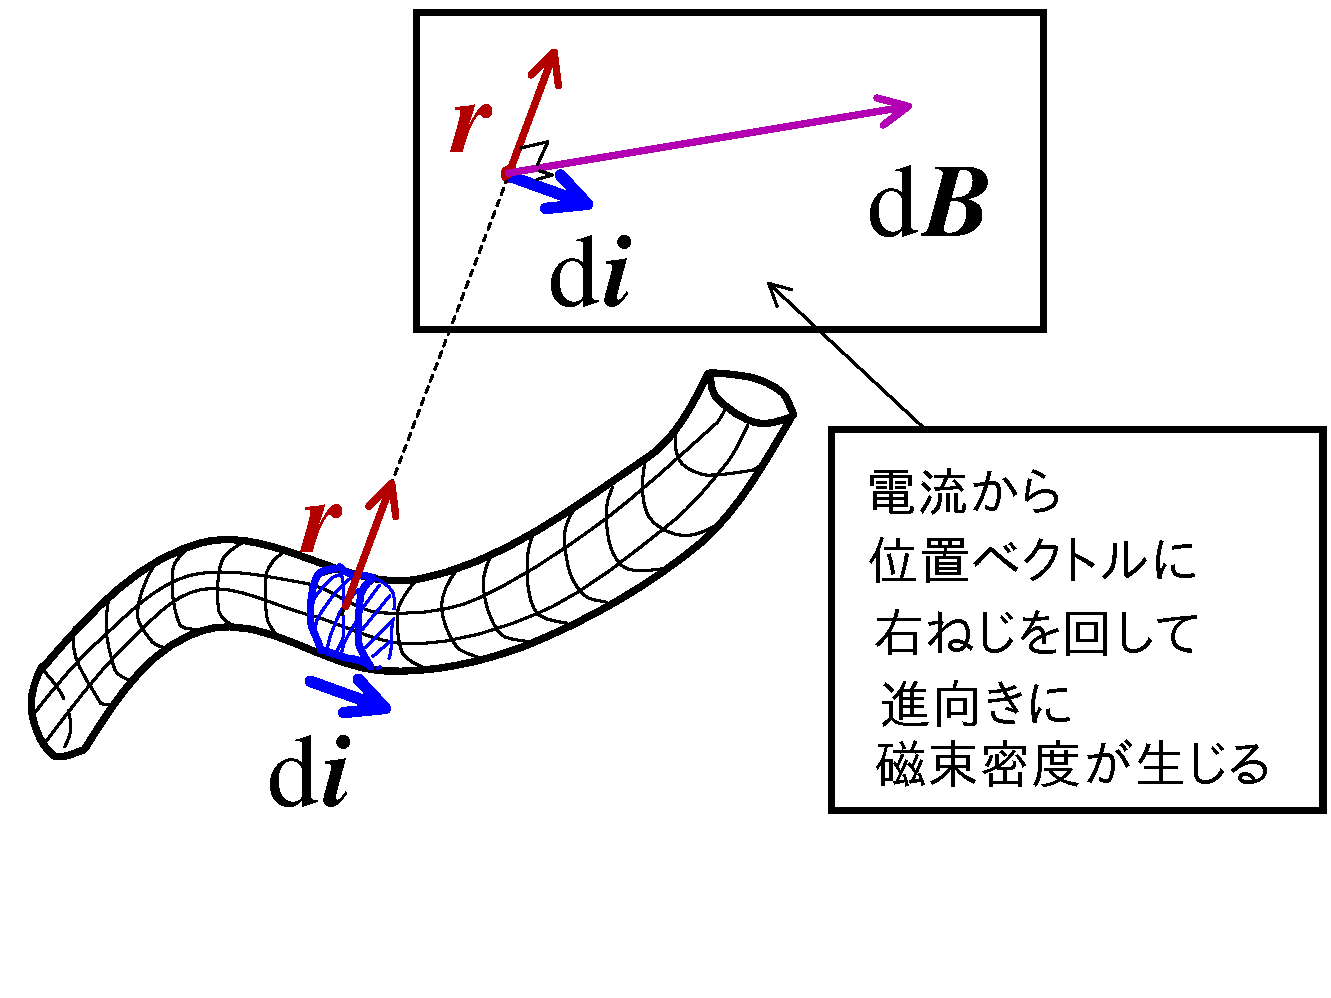
\includegraphics[keepaspectratio, width=7.2cm, height=5.79cm, clip]{biot_savart_1.pdf}
                    \caption{ビオ$=$サバールの法則}
                    \label{fig:biot_savart_1}
                \end{center}
            \end{figure}

    \subsection{点電荷の場合}
    最後に,電気量 $q$ をもつ点電荷に関する表示もしておこう.
    最初に示した式(\ref{Bior=savart'slow1})を思い起こそう.
        \begin{align*}
            \bB(\br)
            &=\frac{\mu_{0}|\bI|}{4\pi}
             \int_{\Gamma}\frac{\bt_{I}(\br')\times
                     (\br-\br')
                   }{|\br-\br'|^{3}}\df s' \\
            &=\frac{\mu_{0}}{4\pi}
             \int_{\Gamma}\frac{\bt_{I}(\br')\times
                     (\br-\br')
                    }{|\br-\br'|^{3}}|\bI|\df s'  \\
            \frac{\df \bB(\br)}{\df s'}
            &=\frac{\mu_{0}}{4\pi}
             \frac{\bt_{I}(\br')\times
                     (\br-\br')
                    }{|\br-\br'|^{3}}|\bI|  \\
            \df \bB(\br)
            &=\frac{\mu_{0}}{4\pi}
             \frac{\bt_{I}(\br')\times
                     (\br-\br')
                    }{|\br-\br'|^{3}}|\bI| \df s'  \\
            &=\frac{\mu_{0}}{4\pi}
             \frac{|\bI|\df s' \bt_{I}(\br')\times
                     (\br-\br')
                    }{|\br-\br'|^{3}}   \\
            &=\frac{\mu_{0}}{4\pi}|\bI|\df s' \bt_{I}(\br')\times
             \frac{(\br-\br')}{|\br-\br'|^{3}}
        \end{align*}

        ここで,\textbf{電流素片} という概念を導入しよう.
        上式の $|\bI|\df s' \bt_{I}(\br')$ に
        注目する.$\df s'$ は導線の微小な長さであるから,
        $|\bI|\df s' \bt_{I}(\br')$ という量は
        電流の微小な一部分であとみなせる.
        この $|\bI|\df s' \bt_{I}(\br')$ のことを電流素片と
        よぶことにしよう
            \footnote{
                教科書によっては,\textbf{電流要素} と表現されることもある.
            }.
        \begin{figure}[hbt]
            \begin{center}
                \includegraphicsdefault{dennryu_sohenn.pdf}
                \caption{電流素片 $|\bI|\df s \bt_{I}(\br)$}
                \label{fig:dennryu_sohenn}
            \end{center}
        \end{figure}


        電流素片 $|\bI| \df s'$ はその極限は,ひとつの点電荷の移動であると
        考えられる.点電荷の電気量を $q$,その速度を $\bv$ とすると,
        \begin{align*}
            |\bI| \df s' = q\bv.
        \end{align*}
        つまり,速度をもった点電荷が作る磁束密度 $\bB(\br)$ は
            \footnote{
                ここで,改めて,$\df \bB(\br)$ を $\bB(\br)$ に表示を置き換える.
                $\df \bB(\br)$ は電流の微小部分の作る磁束密度というイメージであったが,
                今考えている点電荷のつくる磁束密度であるので,それを $\bB(\br)$ と
                表現しても間違いではないだろう.いや,むしろこのように書き換えたほうが,
                式を自然な形にさせることができると思う.
            },
        \begin{align*}
            \bB(\br)
            &=\frac{\mu_{0}}{4\pi}q\bv \times
             \frac{\br-\br'}{|\br-\br'|^{3}}.
        \end{align*}
        \begin{myshadebox}{ビオ$=$サバールの法則(点電荷表示)}
            速度 $\bv$ で運動する,電気量 $q$ をもつ電荷は,次式で表される
            磁束密度 $\bB(\br)$ をその周囲に発生させる.
            \begin{align}
                \bB(\br)
                 &=\frac{\mu_{0}}{4\pi}q\bv \times
                  \frac{\br-\br'}{|\br-\br'|^{3}}.
            \end{align}
        \end{myshadebox}



%===================================================================================================
%  Chapter : 電磁気力(ローレンツ力)
%  説明    : 電磁気学的な力(電磁気力;ローレンツ力)の概念を導入する
%===================================================================================================
\chapter{電磁気力(ローレンツ力)}
%   %-----------------------------------------------------------------------------------------------
%   %  Input
%   %    File Name : PhysNote_EM_1st_LorentzForce.tex
%   %    説明      : クーロン力と磁束密度に関するローレンツ力を統合し,電磁気力を定める.
%   %-----------------------------------------------------------------------------------------------
        
%======================================================================
%  Section
%======================================================================
\section{ローレンツ力(電磁気力)}
    クーロン力 $\bF_{\mathrm{Coulomb}}$ と
    磁束密度に関するローレンツ力 $\bF_{\mathrm{Lorentz}}$ に
    よって,電気的な力と電荷が磁束密度より受ける力を記述する方法を得た.
        \begin{align*}
               & \bF_{\mathrm{Coulomb}} = q\bE. \\
                &\bF_{\mathrm{Lorentz}} = q\bv\times\bB.
        \end{align*}

    ところで,これまで「磁束密度に関するローレンツ力」という表現をしきりに使用
    してきた.わざわざ“磁束密度に関する”なんていう但し書きのような言い回しを
    してきたのには,理由がある.それは,単に \textbf{ローレンツ力} といった
    とき,それは
        \begin{align*}
            \bF &= \bF_{\mathrm{Coulomb}} + \bF_{\mathrm{Lorentz}} \\
                &= q(\bE + \bv\times\bB)
        \end{align*}
    のようなクーロン力と磁束密度に関するローレンツ力の和を指すからである
        \footnote{
            ちなみに,“電場に関するローレンツ力”なんてものは存在しない.ただ,
            磁束密度 $\bB$ や電荷 $q$ が0のときのような場合のローレンツ力は,
            クーロン力と等しくなり,電場に関するローレンツ力といっても間違い
            ではないとは思うが,一般的に通用する語彙ではない.
        }.
    \begin{myshadebox}{ローレンツ力}
        ある空間に電場 $\bE$ と磁束密度 $\bB$ が存在するとき,
        電気量 $q$ をもつ点電荷(以下,電荷 $q$ と書く)が
        速度 $\bv$ で運動しているならば,この電荷 $q$ には
        次式で示す \textbf{ローレンツ力} $\bF$ を受ける.
        \begin{align}
            \bF = q(\bE + \bv\times\bB)
        \end{align}
    \end{myshadebox}

\section{ローレンツ力と観測者}
        このローレンツ力は,不思議な力である.というのも,この力は
        観測者と電荷との相対的な速度 $\bv$ によっているからである.
        同じ電荷を観測していても,観測者によって電荷との相対速度
        が異なるのであれば,ローレンツ力の向きや大きさは,観測者ごとに
        異なったものとなる.なんとも不思議なことであるが,
        相対性理論を受け入れれば,何の不思議なことではなくなる.
        しかし,ここでは電磁気学を学ぶことが目標であるので,
        とりあえず,この不思議さは棚上げにしておき,話を
        先に進めることにしよう.


    \begin{memo}{電荷自身から発する磁束密度}
        電荷が磁束密度中を運動するときには,それにより磁束密度
        に関するローレンツ力を受け,速度の方向が変化してしまう.
        しかし,あとで述べるとおり,アンペールの法則によれば,
        磁束密度の発生源は電流である
            \footnote{
                アンペールの法則(※1)は
                次式で表現される.
                \begin{align*}
                    \drot\bB =  \mu_{0}\left(
                                    \bi + \frac{\rd \bE}{\rd t}
                                \right)
                \end{align*}
                言葉で表現すれば,大雑把に,
                \begin{align*}
                    \mbox{回転する磁束密度} = \mbox{電流} + \mbox{時間変動する電場}
                \end{align*}
                という感じになろう.詳しいことは,後に考える.

                (※1)正確には「アンペール$=$マクスウェルの法則」というべきだ.
            }.

        電荷が速度をもっていれば,
        それは電流と同一視できることになり,つまり,その物体自
        身がその周囲に磁束密度を生じさせていることになる.

        たしかに,はじめに考えたように,速度をもった電荷は,自身が
        発している磁束密度とは発生源が異なる磁束密度の影響をうけて,
        その方向が変化する.しかし一方で,電荷から発している磁束密度
        は,その周囲の磁束密度に影響を与えていることも事実である.

        そうであるとき,その影響はどの程度なのだろうか.それは,
        磁束密度に関するローレンツ力が $q\bv\times\bB$ と表される
        ことから,電荷の電気量 $q$ と速度 $\bv$ の大きさに依存している
        ことは明らかである.

        つまり,電荷を除いた状態での純粋な空間の磁束密度を $\bB_{\mathrm{pure}}$ と
        し,電荷から生じる磁束密度を $\bB_{\mathrm{q}}$ としたならば,電荷が
        存在する場合の正味の空間の磁束密度 $\bB$ は
            \begin{align*}
                \bB = \bB_{\mathrm{pure}} + \bB_{\mathrm{q}} \\
            \end{align*}
        である.だから,電荷が受ける磁束密度に対するローレンツ力は,
            \begin{align*}
                \bF &= q \bv \times \bB \\
                    &= q \bv \times (\bB_{\mathrm{pure}} + \bB_{\mathrm{q}}) \\
                    &= q \bv \times  \bB_{\mathrm{pure}} + q \bv \times \bB_{\mathrm{q}} \\
                \therefore\quad
                \bF &= q \bv \times  \bB_{\mathrm{pure}} + q \bv \times \bB_{\mathrm{q}}
            \end{align*}
        となり,$q \bv \times \bB_{\mathrm{q}}$ という分だけ,周囲の磁束密度を
        変化させ,それが自分の受ける磁束密度に対するローレンツ力に跳ね返ってくる.

        ここで気になるのは,$\bB_{\mathrm{q}}$ である.これは運動している電荷から
        発している磁束密度である.
        大きさはどのくらいで,どの方向に磁束密度は生じているのだろうか.
        これはビオ$=$サバールの法則から,位置 $\br$ に発生させる磁束密度 $\bB(\br)$ は
            \begin{align*}
                \bB_{\mathrm{q}}(\br) =
                \frac{\mu_{0}}{4\pi}q\bv \times
                \frac{\br-\br'}{|\br-\br'|^{3}}.
            \end{align*}
       と計算される.ここに,$\br'$ は磁束密度を観測する固定点である.
       とすれば,電荷が受ける磁束密度に対するローレンツ力は次のようになる.
            \begin{align*}
                \bF &= q \bv \times \bB_{\mathrm{pure}} + q \bv \times
                \left(
                    \frac{\mu_{0}}{4\pi}q\bv \times \frac{\br-\br'}{|\br-\br'|^{3}}
                \right) \\
                &= q \bv \times \bB_{\mathrm{pure}} + \frac{\mu_{0}}{4\pi}
                \left( q^{2} \bv \times \bv \times \frac{\br-\br'}{|\br-\br'|^{3}}
                \right).
            \end{align*}
        結果が見えてきた.ここで,ベクトル解析の公式,任意のベクトル $\bX$ に対して,
        $\bX \times \bX = \bzero$ を思い起こせば,
            \begin{align*}
                \bF &= q \bv \times \bB_{\mathrm{pure}} + \frac{\mu_{0}}{4\pi}
                \left(
                    q^{2} \bzero \times \frac{\br-\br'}{|\br-\br'|^{3}}.
                \right)\\
                &= q \bv \times \bB_{\mathrm{pure}} + \bzero \\
                \therefore\quad
                \bF &= q \bv \times \bB_{\mathrm{pure}}.
            \end{align*}
        この式の意味するところは,明白である.
        運動する電荷から発している磁束密度より受けるローレンツ力は,
        電荷自身に対して影響を及ぼさない,ということである.
        考えて見れば,簡単にイメージができることである.速度をもつ
        電荷がその周囲につくる磁束密度 $\bB_{\mathrm{q}}$ は,その速度に対して垂直な方向に
        生じる.なので,$\bB_{\mathrm{q}}$ は運動する電荷に対して,
        なんのエネルギーも与えないのだ
            \footnote{
                仕事の定義 $W = \bF \cdot \br$ を思い起こそう.物体に仕事を
                すると,それはエネルギーとして蓄えられるのだが,垂直成分は
                それに寄与しない.なぜなら,
                    \begin{equation*}
                        \bF \cdot \br = |\bF||\br| \cos \theta =  |\bF||\br| \cos(\pi/2) = 0.
                    \end{equation*}
            }.
    \end{memo}


%===================================================================================================
%  Chapter : マクスウェル方程式概観
%  説明    : マクスウェル方程式を帰納的に導く
%===================================================================================================
\chapter{マクスウェル方程式概観}
%   %-----------------------------------------------------------------------------------------------
%   %  Input
%   %    File Name : PhysNote_EM_1st_MaxEqImage.tex
%   %    説明      : マクスウェル方程式について,
%   %                その意味するところを言葉で大まかにイメージする
%   %-----------------------------------------------------------------------------------------------
        %   %==========================================================================
%   %  Section
%   %==========================================================================
    \section{4つの基本法則}\label{sec:4fundlaw}
    \begin{mycomment}
        ここでは,真空中の電磁気現象を想定する.言い換えれば,
        物質内のおける電場や磁束密度については想定していない.
        物質が存在する場合の理論は複雑になり,最初に学習する
        際には,理論の骨格を捉えにくいものである.理論の筋道を
        明確に捉えるために,真空中であるという制約を与える.
    \end{mycomment}

%       %======================================================================
%       %  SubSection
%       %======================================================================
        \subsection{はじめに}\label{subseq:4fundlaw_Hajimeni}
        電磁気的現象は4つの基本法則によって説明できる.ニュートン力学
        で言うところの,ニュートンの運動の3法則に対応する部分である.ついでに,
        それに対する方程式も記述しておこう.
            \begin{enumerate}
                \item 電場に対するガウス
                    \footnote{
                        Johann Carl Friedrich Gauss(Gau\ss)(1777--1855, ドイツ)
                        :ドイツの数学者,物理学者.整数や代数についての研究,曲
                        面論などに代表される幾何学の研究が有名である.近代数学の
                        大部分にその業績があり,19世紀最大の数学者とも言われる.
                        また,cgs単位系の「ガウス[G]」は磁気の単位として使われ
                        ている.そのほかにも,「ガウス記号(整数論)」,「ガウス
                        平面(複素関数論)」,「ガウス分布(誤差論)」など彼の名
                        がつけられた概念は多い.
                    }
                    の法則
                    \begin{align}
                        \ddiv \bE = \frac{1}{\varepsilon_{0}}\rho.
                    \end{align}
                \item 磁束密度に対するガウスの法則
                    \begin{align}
                        \ddiv \bB = 0.
                    \end{align}
                \item アンペール
                    =マクスウェル
                    \footnote{
                        James Clerk Maxwell(1831--1879, イギリス):古典電磁気学
                        の理論体系を築いた.この理論より電磁波の予言を行い,ヘル
                        ツ(Heinrich Rudolf Hertz, 1857--1894, ドイツ)らによって
                        実験的に実証された.

                        電磁気学的な自然現象は,4つの法則を基本法則とすることで,
                        説明のつく現象であると提唱する
                        (1865年;A dynamical theory of the electromagnetic field).
                        その後,マクスウェルは,1873年に,電磁気学を体系的に纏めた教科書を
                        出版し,電磁気学を確立させた
                        (1873年;A treatse on electricity and magnetism).
                        この教科書は,電磁気学におけるプリンキピアであると言われるようだ
                        (褒め言葉であると同時に,難解であるという意味も込められているらしい).

                        また,統計物理学の基本的な考え方である,気体分子運動論にかんする
                        研究も行なっている.「マクスウェル分布(マクスウェル--ボルツマン分布)」
                        としても,その名前を残している.これは今日の統計物理学の基礎をなすもの
                        である.

                        また,マクスウェルはキャベンディッシュ(\ref{sec:EM_ObjPreMsg}節の脚注を参照)
                        の仕事を世の中に紹介している.そして,当時新しく設けられた,
                        「キャベンディッシュ研究所」の実験物理学の教授(初代所長)として働いている.
                        なおこの研究所は,上に紹介したキャベンディッシュ(Henry Cavendish)の子孫
                        に当たる,デヴォンシャー第7大公爵が出資して作られた,
                        ケンブリッジ大学の実験物理学施設である.

                        片仮名表記される場合,「マックスウェル」とかかれることもある.

                        (参考1)太田 浩一,『マクスウェルの渦 アインシュタインの時計 現代物理学の源流』,
                        東京大学出版会

                        (参考2)William H.Cropper,『物理学天才外伝』, 講談社(ブルーバックス)
                    }
                    の法則
                    \begin{align}
                        \drot \bB = \mu_{0}\bi + \varepsilon_{0}\mu_{0}\frac{\rd \bE}{\rd t}.
                    \end{align}
                \item ファラデー
                    \footnote{
                        Michael Faraday(1791--1867, イギリス):電磁誘導の発見,
                        電気力線,磁力線の提唱(電磁気現象の近接作用の考え)など,
                        電磁気学に大きい貢献をする.また,化学者としての活躍も有名
                        であり,電気分解の法則の発見がその例である.コンデンサの容
                        量の単位「ファラド[F]」や,ファラデー定数などは,彼の名に
                        ちなんだものである.
                    }
                    の電磁誘導の法則
                    \begin{align}
                        \drot \bE = - \frac{\rd \bB}{\rd t}.
                    \end{align}
            \end{enumerate}

        以下では,これら4つの法則の内容をざっくりと見ていこう.その実験的根拠等の
        細かいことは,次章以降で考えることにする.ここでは,電磁気学は4つの基
        本法則から構成されているのだということを理解してもらいたい.
        各法則が意味する現象の詳細は,後で,それぞれ章を立てて説明する.

        もう一度注意しておこう.先のコメントの部分にも書いたが,以降で想定するのは,
        すべて,真空中で起こる電磁気現象である.物質を含む場合については,また別に
        議論することとにしたい.


%       %======================================================================
%       %  SubSection
%       %======================================================================
        \subsection{電場に対するガウスの法則}
        電場に対するガウスの法則は,電場の発生と消滅に関する法則である.内容は次
        の通りである.
            \\
            \begin{itembox}[l]{\textbf{電場に対するガウスの法則}}
                電場の\textbf{発生源}は\textbf{正に帯電した電荷}である.また,電
                場の\textbf{消滅源}は\textbf{負に帯電した電荷}である.そして,電
                場の発生と消滅は電荷においてのみ起こり,これ以外では起こらない.
            \end{itembox}
            \\

        この法則の意味するところは,電場の発生と消滅の原因は電荷にあることの主張
        である.正に帯電したから電荷から発生した電場は,負に帯電した電荷に吸収(
        消滅)するのである.そして,電場の発生,消滅は電荷以外では起こりえない.
               \begin{figure}[hbt]
                    \begin{tabular}{cc}
                        \begin{minipage}{0.5\hsize}
                            \begin{center}
                                \includegraphicsdouble{GaussLowImage_01.pdf}

                                (A) 正電荷より電場発生
                            \end{center}
                        \end{minipage}
                        \begin{minipage}{0.5\hsize}
                            \begin{center}
                                \includegraphicsdouble{GaussLowImage_02.pdf}

                                (B) 負電荷で電場消滅
                            \end{center}
                        \end{minipage}
                    \end{tabular}
                                \caption{電場に対するガウスの法則}
                                \label{fig:GaussLowImage}
                \end{figure}


%       %======================================================================
%       %  SubSection
%       %======================================================================
        \subsection{磁束密度に対するガウスの法則}
        磁束密度に対するガウスの法則は,磁束密度の発生と消滅に関する法則である.
        内容は次の通りである.
            \\
            \begin{itembox}[l]{\textbf{磁束密度に対するガウスの法則}}
                磁束密度の\textbf{発生源},\textbf{消滅源}は存在しない.
            \end{itembox}
            \\

        磁束密度がある点から生じて,他の点に吸収されるようなことは起こりえない
        ことを,この法則は主張する.つまり,電場の発生源とはる電荷に対応するよう
        な,言わば磁荷は存在しないことを意味する.
                \begin{figure}[hbt]
                    \begin{center}
                        \includegraphicsdefault{GaussLowBImage_01.pdf}
                        \caption{磁束密度に対するガウスの法則}
                        \label{fig:GaussLowBImage_01}
                    \end{center}
                \end{figure}

%       %======================================================================
%       %  SubSection
%       %======================================================================
        \subsection{ファラデーの電磁誘導の法則}
        ファラデーの電磁誘導の法則は,磁束密度の時間的な変化と電場の関係に関する
        法則である.内容は次の通りである.
           \\
           \begin{itembox}[l]{\textbf{ファラデーの電磁誘導の法則}}
               磁束密度が時間的に変化すると,その周囲には回転する電場が発生する.
           \end{itembox}
           \\

        磁束密度とは磁界のことだから,磁界の変化が回転する電場を発生させることに
        なる.具体的な例で考える.磁石は磁界を発生させていることは,中学生なら
        ば誰でもでも知っている.とすれば,磁界が変化する状況を作るには,磁石を手
        で持って振ればよい.ファラデーの電磁誘導の法則の法則は,この手で振ってい
        る磁石の周りに,電場が生じていると主張しているのである.
                \begin{figure}[hbt]
                    \begin{center}
                        \includegraphicsdefault{FaradayLowImage_01.pdf}
                        \caption{ファラデーの電磁誘導の法則}
                        \label{fig:FaradayLowImage_01}
                    \end{center}
                \end{figure}


%       %======================================================================
%       %  SubSection
%       %======================================================================
        \subsection{アンペール$=$マクスウェルの法則}
        アンペール$=$マクスウェルの法則は,電場の時間的な変化と磁束密度に関する法
        則である.内容は次の通りである.
            \\
            \begin{itembox}[l]{\textbf{アンペール$=$マクスウェルの法則}}
                電流の周りには,この電流を取り囲むように回転する磁束密度が生じる.ま
                たこれに加えて電場の状態が時間的に変化すると,その周囲には回転す
                る磁束密度が発生する.
            \end{itembox}
            \\

        電流が流れていると,その周りには磁界が発生しているということは,おそらく
        中学で習うはずだ.この法則では,それに加えて,時間的に変化する電場も,回
        転する磁束密度を作ることを主張している.
                \begin{figure}[hbt]
                    \begin{tabular}{cc}
                        \begin{minipage}{0.5\hsize}
                            \begin{center}
                                \includegraphicsdouble{AMLaw_Image00.pdf}

                                (A) 電流による磁場
                            \end{center}
                        \end{minipage}
                        \begin{minipage}{0.5\hsize}
                            \begin{center}
                                \includegraphicsdouble{AMLaw_Image01.pdf}

                                (B) 電場の時間変化による磁場
                            \end{center}
                        \end{minipage}
                    \end{tabular}
                        \caption{電流と時間変化する電場は,その周囲に回転する磁場を生じる}
                        \label{fig:AMLaw_Image00}
                \end{figure}

%   %==========================================================================
%   %  Section
%   %==========================================================================
    \section{マクスウェル方程式を見てみよう}
        \begin{mycomment}
            この節では,マクスウェル方程式を実際に見てみよう.
            だたし,その式をイメージとして捉え,意味すること
            を重視する.数式の本来の性質等は,各法則毎に詳しく
            調べることにし,ここでは数式の形に慣れることが目的
            である.徐々にマクスウェル方程式に馴染んで行こう.
        \end{mycomment}

%       %======================================================================
%       %  SubSection
%       %======================================================================
        \subsection{「マクスウェル方程式」とは}
        \begin{mycomment}
            まずは,「マクスウェル方程式」と言われる式について説明する.
            実は,マクスウェル方程式と言われてはいるが,マクスウェルがその
            方程式を発見したのではない.勘違いを起こしてしまいがちだが,
            マクスウェルが発見したという意味での,方程式は存在しないのである.
            ではどういうことかというと,言うなれば,
               “マクスウェルが提唱した,電磁気の公理的な4つの連立方程式”
            がマクスウェル方程式と呼ばれるものである.
        \end{mycomment}

%           %==================================================================
%           %  SubsubSection
%           %==================================================================
            \subsubsection{マクスウェルが電磁気学を確立する}
            電磁気的な自然現象には,冬場に発生する静電気や,より身近なものとして,
            磁石がある.携帯電話や無線LANも電磁気現象(電磁波)を利用した装置である.
            電磁気的な現象は,一見すると,その発生機構が複雑であるように感じてしまう.
            たしかに,マクスウェルにより指摘される以前では,電磁気現象は複雑であると
            感じることだったろう.しかし,今では,電磁気現象は,たった4つの法則を認め
            るだけで,説明ができることが分かっている.これを指摘した人物
            こそマクスウェルである.

            マクスウェルの提唱した4つの法則は,それ以前に先人
                \footnote{
                    例えば,アンペール,クーロンなどがいる.
                }
            により発見されていた自然現象をピックアップしたものであり,つまり,
            マクスウェル自身が4つの法則を発見したわけではない.マクスウェルの偉大なところ
            は,それまで煩雑としていた電磁気現象に関する実験結果(実験法則)を,体系化した
            ことにある.それまでには,色々な電磁気学の実験が行われて,その実験結果も
            多様にあったはずである.マクスウェルは,この煩雑な実験結果は,4つの自然現象
            を受け入れることで,すべてが上手く(数学的に)説明できることを示唆した.

%           %==================================================================
%           %  SubsubSection
%           %==================================================================
            \subsubsection{数式で表現してこそ,基本法則と言える}
            マクスウェルが基本法則として取り上げた4つの実験結果については,定性的には,
            上で紹介しと通りである(\ref{sec:4fundlaw}節参照).しかし,これらの法則は,
            数式により表現してこそ,意味を成す
                \footnote{
                    物理現象を説明するには,数式によりそれを表現すべきだ.
                    数式で表されて,初めて,詳細な推論や論理的思考が可能になるからだ.
                    数式を用いずに,言葉で表現しても論理的推論が不可能というわけではないが,
                    考えにくいし,論理もわかりにくくなる.数式で表現できれば,論理的
                    推論もしやすくなるし,論旨もわかりやすくなる.
                    不慣れな数式を扱うことが億劫かもしれなが,ここは少々なれるまで我慢
                    してもらいたい.物理学は数式を扱う学問なので,数式に慣れることは大事だ.
                    4つの法則で電磁気学現象を説明できるといったのは,各法則を方程式
                    で表したときに,電磁気現象が4つの方程式から数学的演算により,
                    論理的必然性をもった結果として導かれることをいう.
                }.
            そこで,次に,4つの基本法則を表す数式を紹介する.ただし,その数式に深入り
            することはせず,そのイメージを捉えることを第一の目的としたい.より詳しいことは,
            次章以降で考える
                \footnote{
                    実は,以下に説明する4つの方程式の理解こそが,初めて電磁気学を学ぶ際の
                    目標なのである.つまり,ここでは,その最終目標を先回りして紹介すること
                    になる.これは,学習の目標を明確にすることを考えてのことである.目標が
                    明確になれば,学習の際の不安(何をしているのかが分からないなど)も,少
                    しは解消されることと思う.
                }.

%           %==================================================================
%           %  SubsubSection
%           %==================================================================
            \subsubsection{マクスウェル方程式の2種類の表現}
            マクスウェル方程式は4つであるが,実は,その表現方法が2種類があり,
            微分を使って表現したものが \textbf{微分形},
            積分を使って表現したものが \textbf{積分形} と言われる.ここでは,
            この2種類の表現方法を紹介する.微分形と積分形の違いは,視点の違いである.
            現実に起こっている現象を肌で感じる場合には,積分形の方程式を用いる.
            そのため,工学の分野では,積分形を使うことのほうが多いと思う.これに対し,
            微分形で記述されたものは,現象を局所的に見た場合に使われる.微分形は
            理論的考察を行う場合に使うことが多い.もちろん,積分形で表されようが,
            微分形で表されようが,その式は全く等価である(当たり前のはずだが,念のために).


%       %======================================================================
%       %  SubSection
%       %======================================================================
        \subsection{約束:独立変数の記述の省略}
                マクスウェル方程式は,位置 $\br$ と時間 $t$ の4つの独立変数を
                含む関数の間に成り立つ式であるが,この独立変数をいちいち明記
                していたら,式が煩雑になり見難くなっていしまう.そこで,
                以下のように,独立変数を省略して記述する.
                すなわち,
                電場 $\bE$,磁束密度 $\bB$,電流密度 $\bi$,電荷密度 $\rho$ であり,
                その意味は次式の通り.
                    \begin{align*}
                        \bE  &= \bE(\br,\,t) \\
                        \bB  &= \bB(\br,\,t) \\
                        \bi  &= \bi(\br,\,t) \\
                        \rho &= \rho(\br,\,t)
                    \end{align*}
                また,$\varepsilon_{0}$,$\mu_{0}$ は,それぞれ,真空中の誘電率,透磁率と言われる,
                スカラー量で,単なる定数である(位置と時間の関数ではない).

                ついでに,他の記号も説明する.
                任意の閉曲面を $S$ で表現する.また,$S$ で囲まれた内部の領域全体を $\Omega_{S}$ と
                書く.閉曲面の微小部分は $\df S$ であり,
                $\df S$ の単位法線ベクトルは $\bn:=\bn(\br,\,t)$ で表現する.
                また,$l$ は任意の閉経路(ループしている経路,輪状の経路のこと)である.そして,$S_{l}$ というのは,
                閉経路 $l$ を縁とする開曲面を表す.そして,閉経路 $l$ の単位接線ベクトルを $\bt:=\bt(\br,\,t)$ と
                表現する.

                くどいかもしれないが,演算に関する記述方法の説明もしておこう.
                $\sint_{S} X\df S$ は,関数 $X$ を,$S$ に対して面積分を行うことを意味する.また,
                $\vint_{\Omega_{S}} X \df V$ は,関数 $X$ を,$S$ の内側の全領域 $\Omega_{S}$ に
                対して体積分を行うことを意味する.

%       %======================================================================
%       %  SubSection
%       %======================================================================
        \subsection{マクスウェル方程式(微分形)}
        \begin{mycomment}
            上では,現実に起こっている法則のイメージを説明したが,
            ここではもう一歩先に進んで数式を眺めてみよう.この節では,
            微分形のマクスウェル方程式を確認する.積分形も,後で確認する.
            何度も言うが,
            数式そのものを理解することが目的ではなく,数式のイメージを
            持つことが目的である.数式の詳細は後で述べる.ここではとにかく,
            求めるべきマクスウェル方程式がどのようなものかを,感覚的に
            把握してもらいたい.
        \end{mycomment}
%           %==================================================================
%           %  SubsubSection
%           %==================================================================
            \subsubsection{電場に対するガウスの法則の式:微分形}
            \begin{mysmallsec}{数式}
                電場に対するガウスの法則の,微分形の式は次式の通り.
                \begin{align}
                    \ddiv \bE = \frac{1}{\varepsilon_{0}}\rho.
                \end{align}
            \end{mysmallsec}

            \begin{mysmallsec}{法則のイメージ}
                電場の発生あるいは消滅は,電荷の存在する場所で生じる.また,言い換えれば,
                ある場所において,電場が発生あるいは消滅していることと,その場所に電荷が
                存在することは,同じ意味をなす.

                ベクトル $\bE$ は電場で,その前に書かれている $\ddiv$ は,
                divergence(発散) を意味する.なので,左辺 $\ddiv \bE$ は電場の発散を表す.
                右辺の$\rho$ は電荷密度
                    \footnote{
                        1/$\varepsilon_{0}$ がかかっているが,単なる比例定数である.
                        これは単位系としてSI単位を採用していることによって現れた定数
                        であり,式の表す物理的イメージにはあまり関係がないと思って良い.
                    }
                であり,電荷密度の存在が表されている.
                電場の発散と電荷密度が等号で結ぶことによって意味されることは,
                「電荷密度が存在すれば,その周囲には電場の発散が生じる」ということである.
                更にその逆もいうことができて,「電場の発散の原因は電荷密度である」ということも
                できる.
                電場の発生あるいは消滅は,電荷の存在しない場所では,絶対に発生しない.
            \end{mysmallsec}

                \begin{figure}[hbt]
                    \begin{center}
                        \includegraphicsdefault{GaussLowEImage_03.pdf}
                        \caption{電場は電荷より生じる}
                        \label{fig:GaussLowEImage_03}
                    \end{center}
                \end{figure}

%           %==================================================================
%           %  SubsubSection
%           %==================================================================
            \subsubsection{磁束密度に対するガウスの法則の式:微分形}
            \begin{mysmallsec}{数式}
                磁束密度に対するガウスの法則の,微分形の式は次式の通り.
                \begin{align}
                    \ddiv \bB = 0.
                \end{align}
            \end{mysmallsec}

            \begin{mysmallsec}{法則のイメージ}
                この式は,磁束密度はどこからも湧き出しがないことを表現している.
                見方を変えれば,ある部分で湧き出す磁束密度の量と,その部分で消滅する
                磁束密度の量が等しいから,正味として湧き出しがないとみなされる.

                つまり,磁束密度の発生場所を特定することはできないということである.
                こういう言い方すると,“磁束密度は存在して,その発生原因は電流にあることを,
                先に説明している.つまり,発生している場所を示すことができるではないか”と
                いう疑問を持たれてしまうかもしれない
                    \footnote{
                        少なくとも,私はそう思った.
                    }.
                しかし,これは言葉の意味の捉え方(あるいは記述の仕方)の問題であり,
                磁束密度の存在場所が特定できないことを言っているのではない.この法則は
                ,あくまでも,発生源を特定することができないということであり,発生して
                いる場所を示せないということではない.現に,磁石の周囲には磁束密度が存在
                していることは,すでに知っていることである.たしかに,磁石から磁束密度が
                湧き出していると考えても,間違いではないが,この法則の言っている「湧き出し」とは
                意味がことなる.先にも書いたとおり,ここで言う「湧き出し」とは,磁束密度の
                生じる量と消滅する量の,“正味の湧き出し”ということである.この正味の湧き出しが
                0であるというとは,この世界のどの場所を見ても磁束密度の正味の湧き出しがないという
                ことを意味しているのである.この「正味の」という部分に,注意すべきだ.
            \end{mysmallsec}

                \begin{figure}[hbt]
                    \begin{center}
                        \includegraphicsdefault{GaussLowBImage_02.pdf}
                        \caption{磁束密度の湧き出しはない}
                        \label{fig:GaussLowBImage_02}
                    \end{center}
                \end{figure}


%           %==================================================================
%           %  SubsubSection
%           %==================================================================
            \subsubsection{アンペール$=$マクスウェルの法則の式:微分形}
            \begin{mysmallsec}{数式}
                アンペール$=$マクスウェルの法則の式の,微分形の式は次式の通り.
                \begin{align}
                    \drot \bB = \mu_{0}\bi + \varepsilon_{0}\mu_{0}\frac{\rd \bE}{\rd t}.
                \end{align}
            \end{mysmallsec}

            \begin{mysmallsec}{法則のイメージ}
                右辺に項が2つあるが,これらはそれぞれ,意味することが異なる.
                右辺の第一項は,電流が磁場を作るということを主張するものである.
                これは,アンペールの法則とよばれる
                    \footnote{
                        アンペールの法則とは,上式の第二項が常に0である場合のことである.
                        すなわち,次式がアンペールの法則を表す式である.
                            \begin{align}
                                \drot \bB = \mu_{0}\bi.
                            \end{align}
                        アンペールの法則の意味するところは,式を見れば明らかである.
                        口うるさく意味を説明すれば,
                        「回転している磁束密度が存在するということは,その内側の領域に
                        電流が生じていることを意味する」ということだ.
                    }.
                そして,第二項が意味するのが,
                \textbf{変位電流} という概念である.詳細は後述するが,ここでは,
                おおよそのイメージとして,電場の時間変化がその周囲に磁束密度を
                生じさせる,と解釈して欲しい
                    \footnote{
                        式をそのまま言葉にしただけである.その真意の程は後の記述を
                        参照.
                    }.

                なぜ,「変位電流」を導入する必要があるのかというと,単なるアンペールの法則が
                電荷保存則に矛盾してしまうからである.つまり,アンペールの法則と電荷保存則の
                どちらかが,間違っている(不完全である)可能性があるということである
                    \footnote{
                        あるいは,どちらとも間違いなのかもしれない.しかしこの可能性は,
                        あとに記述する,マクスウェルの修正によってなくなる.
                    }.
                マクスウェルによる回答は,アンペールの法則が不完全である,ということだった.
                そして,マクスウェルはアンペールの法則を完全な形にすべく,「変位電流」という
                新しい概念を考案し,アンペールの法則にそれを組み込むことで,電荷保存則との
                矛盾を解消したのである.

                あとに分かることだが,この変位電流は,ファラデーが発見する電磁誘導の法則
                に対をなす現象である,と見ることもできる.この変位電流と電磁誘導とにより,
                電磁波という現象が起こるのである.電磁波についても,後ほど考えることにしたい
                    \footnote{
                        マクスウェル方程式の偉大さの一つは,電磁波の存在を予言したことである.
                    }.

                もう一度改めて,この法則の内容を確認しておこう.電流はその周囲に磁束密度を
                発生させる.さらに,それに加えて,電場の時間変化が起きた際にも,その電場の
                変化にともなって,その周囲に,磁束密度が生じるのである.
            \end{mysmallsec}

                \begin{figure}[hbt]
                    \begin{tabular}{cc}
                        \begin{minipage}{0.5\hsize}
                            \begin{center}
                                \includegraphicsdouble{dennryu_to_jisokumitudo.pdf}

                                (A) 電流による磁場
                            \end{center}
                        \end{minipage}
                        \begin{minipage}{0.5\hsize}
                            \begin{center}
                                \includegraphicsdouble{hennnidenryu_to_jisokumitudo.pdf}

                                (B) 変位電流による磁場
                            \end{center}
                        \end{minipage}
                    \end{tabular}
                        \caption{電流,変位電流と磁束密度の関係}
                        \label{fig:I_i_B}
                \end{figure}


%           %==================================================================
%           %  SubsubSection
%           %==================================================================
            \subsubsection{ファラデーの電磁誘導の法則の式:微分形}
            \begin{mysmallsec}{数式}
                ファラデーの電磁誘導の法則の式の,微分形の式は次式の通り.
                \begin{align}
                    \drot \bE = - \frac{\rd \bB}{\rd t}.
                \end{align}
            \end{mysmallsec}

            \begin{mysmallsec}{法則のイメージ}
                左辺は回転する電場を表している.右辺は負の符号がついて入るが,
                磁束密度の時間変化が記述されている.渦を巻くように電場が生じている
                ならば,その周囲に磁束密度の時間変化が起こっているということを示している.
                また,言い方を変えれば,磁束密度が時間変化するとき,その周囲に渦を巻くようにして
                電場が生じるということでもある.磁束密度の時間変化とは,現実的に言えば,例えば
                磁石を左右に振った場合のことである.このとき左右にふった磁石の周りには,その磁石を
                取り囲むように,渦電場が生じるのである.
            \end{mysmallsec}

%       %======================================================================
%       %  SubSection
%       %======================================================================
        \subsection{マクスウェル方程式(積分形)}
%           %==================================================================
%           %  SubsubSection
%           %==================================================================
            \subsubsection{電場に対するガウスの法則の式:積分形}
            \begin{mysmallsec}{数式}
                電場に対するガウスの法則の,積分形の式は次式の通り.
                \begin{align}
                    \sint_{S} \bE \cdot \bn \df S = \frac{1}{\varepsilon_{0}} \vint_{\Omega_{S}} \rho \df V.
                \end{align}
            \end{mysmallsec}

            \begin{mysmallsec}{法則のイメージ}
                この式の言っていることは,微分形のそれと同じだが,次のような
                イメージを連想させる.すなわち,ある領域 $S$ から電場が湧き出ている
                ならば,その内部領域 $\Omega_{S}$ に電荷が存在しする.そして,このとき湧き出す電場の量
                は,$\Omega_{S}$ 内に存在するすべての電荷の電気量の総和
                を $\varepsilon_{0}$(真空中の誘電率;詳細は後述する)で割った値に等しい.

                要するに,ある領域から電場が生じているのであれば,その領域には
                必ず電荷が存在するということである.
            \end{mysmallsec}

%           %==================================================================
%           %  SubsubSection
%           %==================================================================
            \subsubsection{磁束密度に対するガウスの法則の式:積分形}
            \begin{mysmallsec}{数式}
                磁束密度に対するガウスの法則の,積分形の式は次式の通り.
                \begin{align}
                    \sint_{S} \bB \cdot \bn \df S = 0.
                \end{align}
            \end{mysmallsec}

            \begin{mysmallsec}{法則のイメージ}
                この式の意味は,微分形のそれと全く同様である.

                この表現のほうが,イメージしやすいかもしれない.任意の領域 $S$ を
                設定しても,そこから生じる正味の磁束密度の量は0であることを,
                表現している.つまり,磁束密度の湧き出し場所が,$S$ 内部ではない
                ということである.といっても,湧き出しはどこか別の場所($S$ の外側)に
                あるということではない.$S$ は任意に設定できる閉曲面であるから,
                $S$ をどんな風にとっても,磁束密度の発生源は $S$ の内部ではないという
                ことになる.つまり,この世界の至る場所で,磁束密度の湧き出し量が
                正味0であるということだ.

                電場に対するガウスの法則は,電場の発生原因を電荷に押し付けいているのに対し,
                磁束密度に対するこの法則は,いわば「磁荷」が存在しないということを意味する.
                磁束密度に対して,なぜ「磁荷」がないのだろうかといった疑問も強いことと思う.
                実際,物理学者の中でもその存在を信じ,探している人もいるらしい.しかし,
                このノートでは,この現象を実験事実として認め,深入りは避けることとしたい
                    \footnote{
                        実は,特殊相対性理論を学習すると,磁束密度は,光速不変の原理と
                        特殊相対性理論から導かれるローレンツ力と,クーロンの法則から導
                        出することができてしまう.電場の発生原因は電荷にあり,電荷はク
                        ーロンの法則に従った動きをする.他方,物体が光の速さで運動する
                        さいには,ローレンツ変換に従う.とどの詰まりは,電荷が光速で運
                        動する際に,静止している観測者には,その周囲に磁束密度が分布し
                        ているようにみえてしまうのである.これは,ローレンツ力に関連す
                        る.先に,ローレンツ力は,観測者と電荷との相対速度 $\bv$ が関
                        係していることを見た.この相対速度こそが,磁束密度の存在を支え
                        ているのである.磁束密度は,観測者と電荷の相対的な関係により,
                        生じるものであると,考えることもできるのである.このことを定量
                        的に考えることは,相対論を学習した後で行うことにしよう.
                    }.
            \end{mysmallsec}

%           %==================================================================
%           %  SubsubSection
%           %==================================================================
            \subsubsection{アンペール$=$マクスウェルの法則の式:積分形}
            \begin{mysmallsec}{数式}
                アンペール$=$マクスウェルの法則の式の,積分形の式は次式の通り.
                \begin{align}
                    \oint_{l} \bB \cdot \bt \df l
                    = \sint_{S_{l}} \left( \bi + \varepsilon_{0}\frac{\rd \bE}{\rd t} \right) \cdot \bn \df S_{l}.
                \end{align}
            \end{mysmallsec}

            \begin{mysmallsec}{法則のイメージ}
                この式の意味するところは,ある閉曲線 $l$ の内側を観察したとき,
                磁束密度が生じているのであれば,$l$ を境界とする曲面 $S_{l}$ を
                電流が貫いているか,もしくは電場の時間変化が生じているということ
                である.電場の時間変化と電流は,その周囲に磁束密度を発生させるのである.

                この積分形の式の左辺により,生じる磁束密度の総量が計算される.右辺は,
                閉曲面 $S_{l}$ に生じている全電流と電場の時間変化の総量が計算される.
                つまり,全電流と電場の時間変化の総量を計算することで,生じる磁束密度の総量
                がわかるのである.
            \end{mysmallsec}

%           %==================================================================
%           %  SubsubSection
%           %==================================================================
            \subsubsection{ファラデーの電磁誘導の法則の式:積分形}
            \begin{mysmallsec}{数式}
                ファラデーの電磁誘導の法則の式の,積分形の式は次式の通り.
                \begin{align}
                    \oint_{l} \bE \cdot \bt \df l
                    = -\frac{\rd}{\rd t} \sint_{S_{l}} \bB \cdot \bn \df S_{l}.
                \end{align}
            \end{mysmallsec}

            \begin{mysmallsec}{法則のイメージ}
                磁束密度の時間変化は,その周囲に回転する電場を発生させることを,
                この式は意味している.

                微分形の式は,生じているか否かを判定するものであるが,
                この積分形の式は,生じる電場の総量が計算できる.
                閉ループ $l$ に導線を重ねあわせて導線の輪を作り,
                その導線の輪の内側において磁束密度を変化させると,
                導線に起電力が生じる.この起電力の大きさは,どの程度磁束密度を
                変化させたかによって決まる.その計算式が,積分形の電磁誘導の法則の
                式である.
            \end{mysmallsec}


%===================================================================================================
%  Chapter : 電場に対するガウスの法則
%  説明    : 電場に対するガウスの法則をクーロンの法則から導く
%===================================================================================================
\chapter{電場に対するガウスの法則}
%   %-----------------------------------------------------------------------------------------------
%   %  Input
%   %    File Name : PhysNote_EM_1st_GaussLowEF.tex
%   %-----------------------------------------------------------------------------------------------
        %   %==========================================================================
%   %  Section
%   %==========================================================================
    \section{電場の定義}
    \subsection{クーロンの法則(復習)}
        \begin{mycomment}
            クーロンの法則についての詳細は,\ref{sec:CoulomnbForce}節を参照.
            以下は,そこからの抜粋である.
        \end{mycomment}

            ここに,電荷が2つあるとしよう.この2つの電荷は区別する
            ことができて,$q_{1}$,$q_{2}$ という電気量を持っている
            とする.電荷 $q_{1}$ と $q_{2}$ との距離を $r$ としたと
            き,この2つの電荷が受ける力は,以下のような規則がある.
            \begin{itemize}
                \item 2つの電荷の電気量が互いに異なる符号をもってい
                      るならば,両電荷は互いに引き合う向きに力を受
                      ける
                \item 2つの電荷の電気量が同じ符号を持っているならば,
                      両電荷は互いに反発しあう向きに力を受ける.
                \item 2つの電荷の受ける力の大きさは等しく,
                      向きは互いに逆向きである
                \item 2つの電荷が受ける力の大きさは,
                      2つの電荷の電気量の積($q_{1}q_{2}$)に比例する.
                \item 2つの電荷が受ける力の大きさは,
                      2つの電荷間の距離の2乗($r^{2}$)に反比例する.
            \end{itemize}

        図\ref{fig:coulombs_low}をもう一度載せておこう.
        \begin{figure}[hbt]
            \begin{tabular}{cc}
                \begin{minipage}{0.5\hsize}
                    \begin{center}
                        \includegraphicsdouble{coulombs_low1.pdf}
                    \end{center}
                \end{minipage}
                \begin{minipage}{0.5\hsize}
                    \begin{center}
                        \includegraphicsdouble{coulombs_low2.pdf}
                    \end{center}
                \end{minipage}
            \end{tabular}
        \end{figure}


            次の数式によって,クーロンの法則は表現される.

            電荷 $q_{1}$ に対して働く力は,以下.
               \begin{align}\label{eq:coulomb_force_f1_2nd}
                   \bF_{21} =
                       \frac{1}{4\pi\varepsilon_{0}} \frac{q_{1}q_{2}}{r^{2}}
                           \frac{\br_{1} - \br_{2}}{|\br_{1} - \br_{2}|}.
               \end{align}

            電荷 $q_{2}$ に対して働く力は,以下.
               \begin{align}
                   \bF_{2} = -\bF_{1} =
                       \frac{1}{4\pi\varepsilon_{0}} \frac{q_{2}q_{1}}{r^{2}}
                           \frac{\br_{2} - \br_{1}}{|\br_{2} - \br_{1}|}.
               \end{align}


        \begin{figure}[hbt]
            \begin{center}
                \includegraphicsdefault{Coulombs_Force.pdf}
            \end{center}
        \end{figure}


%   %==========================================================================
%   %  Subsection
%   %==========================================================================
    \subsection{電場に対するガウスの法則の導出}
        \begin{mycomment}
            ガウスの法則は,言っていることは単純だが,数式を用いて説明されると,
            慣れないうちは何のことだかサッパリわからないことだろう.なので,
            どの教科書でも取られている手段だが,まずは単純な場合から考えて,
            徐々に一般化していこう.まず,点電荷1個より生じる電場の満たす
            法則を考える.次に,電荷の個数を増やし,$N$ 個の点電荷にする.
            最後に,最も一般的な連続分布する電荷より生じる電場の満たす法則を
            考える.また,電場のみが存在し,磁束密度は存在しないとして,
            議論が煩雑になるのを避けることとする
                \footnote{
                    このような仮定をすることに,注意しておこう.
                    時間的に変動する電磁場についてはこのように考えることはできない,
                    ということである.理由は,判例を示すのが手っ取り早い.
                    中学生のときに, \textbf{電磁誘導の法則} に
                    よって,『磁石を動かしたときに,電流が生じる』という現象を
                    観測した(はずである).磁石を動かすことは
                    磁束密度を変化させることを意味し,
                    電流が発生するということは導体内に
                    電場が生じたということになる.
                    つまり,磁束密度が時間的に変化すると,電場が発生するのである.
                    このことを考えると,動電磁場の場合は電場と磁束密度を
                    分けて考えることはできないのである.電磁誘導の法則についての詳しいことは,動電磁場の
                    部分で確認する.
                }.
        \end{mycomment}
%       %======================================================================
%       %  Subsection
%       %======================================================================
        \subsubsection{クーロンの法則から見えてくること}
            クーロンの法則によって定義された電場 が満たしている法則を考える.
            2つの点電荷における,クーロンの法則を書き下そう.
                \begin{align}
                    F  =  \frac{1}{4\pi \varepsilon_{0} } \frac{q_{1}q_{2}}{r^{2}}.
                \end{align}
            ここに,$q_{1}$,$q_{2}$ は電荷の電気量であり,$r$ は
            2つの点電荷間の距離である.ここでは,大きさのみを考える.
            さてこの時,電気量 $q_{1}$ をもつ電荷が作る電場を考えると,
                \begin{align}
                    E_{1}  =  \frac{1}{4\pi \varepsilon_{0}} \frac{q_{1}}{r^{2}}.
                \end{align}
            いま,興味があるのは,この電場 $E_{1}$ が満たす法則である.
            次のように書き変えてみよう.
                \begin{equation*}
                    E_{1}  =  \frac{1}{4\pi \varepsilon_{0}} \frac{q_{1}}{r^{2}}
                            =  \frac{1}{4\pi r^{2}} \frac{q_{1}}{\varepsilon_{0}}
                \end{equation*}
            さて,この式の $4\pi r^{2}$ の部分に注目する.これは,球の
            表面積の公式と同じである.そこで,これを球の表面積
            としてみなし,記号 $S$ で置き換えてみよう.
                \begin{equation*}
                    E_{1}  =  \frac{1}{S} \frac{q_{1}}{\varepsilon_{0}}
                \end{equation*}
            両辺に $S$ をかける.
                \begin{equation*}
                    E_{1}S  =   \frac{q_{1}}{\varepsilon_{0}}
                \end{equation*}

            ところで,球の面積 $S$ は,積分記号を用いて面積分
            の形で表現すると,
                \begin{equation*}
                    S = \int_{S} \df S
                \end{equation*}
            である.$S$ は球の表面全体を表すと同時に,その表面積でもある.球の
            表面である $S$ を微小分割して,かき集めたものが,
            球の面積である.
            これを用いると,電場の式は
                \begin{equation*}
                    E_{1}\int_{S} \df S  =   \frac{q_{1}}{\varepsilon_{0}}
                \end{equation*}
            となる.
            さて,球の面の法線ベクトルと点電荷が作る電場の向きは,
            球のどの部分でも一致する.しがって,上式の電場 $E_{1}$ は,
            球の面積積分の中に入れてさしつつ変えない.つまり,
                \begin{equation*}
                    \int_{S} E_{1}\df S  =   \frac{q_{1}}{\varepsilon_{0}}
                \end{equation*}
            とできる.

            実は,この式が求めている式なのである.
            すなわち,上式が電場が従う法則である.
            言葉で表せば,次のようになる:点電荷 $q_{1}$ が
            球面 $S$ の内部に存在するとき,
            その周囲につく電場 $E_{1}$ を球面 $S$ で面積分すると,
            $q_{1}/\varepsilon_{0}$ という値になる.

            この法則を,\textbf{ガウスの法則} という.
            しかし,今得られたガウスの法則を,さらに一般化することが
            できる.次の項目で,このガウスの法則を一般化しよう.

%       %======================================================================
%       %  Subsection
%       %======================================================================
        \subsubsection{1つの点電荷のみが存在する場合}
            点電荷が1個しかない状況を想定し(図\ref{fig:Gauss_1tendenka}),
            この1個の点電荷から生じる電場が満たす法則について考える.
                        \begin{figure}[hbt]
                            \begin{center}
                                \includegraphicsdefault{Gauss_1tendenka.pdf}
                                \caption{閉曲面$S$の中に1つの電荷を含む場合}
                                \label{fig:Gauss_1tendenka}
                            \end{center}
                        \end{figure}

            1つの点電荷が作る電場を書き下すと,
                \begin{align}
                    \bE(\br)
                    &=\frac{1}{4\pi\varepsilon_{0}}\int_{\Omega_{S}}
                    \frac{q\delta(\br-\br^{*})}
                         {|\br-\br^{*}|^{2}}
                    \frac{\br-\br^{*}}
                         {|\br-\br^{*}|}\df V^{*}
                \end{align}
            である.(電場の定義式(\ref{denba})
            で $\rho(\br^{*})
            =q\delta(\br-\br^{*})$ と置けばよい.)
            ここで, $1/4\pi\varepsilon_{0}$ は定数であるので積分記号の前に出した.
            点電荷の位置を $\br^{*}$ として,$\br^{*}=0$ と
            原点を定める.すると,
                \begin{align*}
                    \bE(\br)
                    &=\frac{1}{4\pi\varepsilon_{0}}
                    \frac{\displaystyle\int_{\Omega_{S}}
                    q\delta(\br)\df V}{|\br|^{2}}
                    \frac{\br}
                         {|\br|}  \\  \\
                    &=\frac{1}{4\pi\varepsilon_{0}} \int_{\Omega_{S}}
                    q\delta(\br)\df V
                    \frac{1}{|\br|^{2}}
                    \frac{\br}
                         {|\br|}
                \end{align*}
            と書ける.この式の両辺を,$\Omega_{S}$ の表面である閉曲面 $S$ で面積分する.
                \begin{align*}
                    &\int_{S}\bE(\br)\cdot\textit{\textbf{n}}(\br)\df S \\
                    &=\frac{1}{4\pi\varepsilon_{0}}
                    \int_{S}\left( \int_{\Omega_{S}} q\delta(\br)\df V \right)
                    \frac{1}{|\br|^{2}}
                    \frac{\br}
                         {|\br|}\cdot\textit{\textbf{n}}(\br)\df S.
                \end{align*}
            この場合,右辺の体積積分と面積分 は関係がないので
                \footnote{
                        体積積分を先に計算する必要があり,この体積積分の部分は定数になる.
                },体積積分を
            面積分の外に出すことができる.
            この式の体積積分の部分は,系の電気量の総和を計算するものであり,定数であると考えられるのである.
                \begin{align*}
                    &\int_{S}\bE(\br)\cdot\textit{\textbf{n}}(\br)\df S \\
                    &=
                    \frac{1}{4\pi\varepsilon_{0}}
                    \left(\int_{\Omega _{S}}q\delta(\br)\df V \right)
                    \left(\int_{S} \frac{1}{|\br|^{2}}
                    \frac{\br}{|\br|} \cdot \textit{\textbf{n}}(\br)\df S \right) \\
                    &=
                    \frac{1}{4\pi\varepsilon_{0}}
                    \left(\int_{\Omega _{S}}q\delta(\br)\df V \right)
                    \left(\int_{S} \frac{\br}{|\br|^{3}}
                    \cdot \textit{\textbf{n}}(\br)\df S \right).
                \end{align*}
            ここで,公式
                    \begin{align}
                        \int_{S}\frac{\br}{|\br|^{3}}
                        \cdot\textit{\textbf{n}}(\br)\df S&=4\pi\qquad S\supset 0(=\br^{*})
                    \end{align}
            を用いると $4\pi$ が消えて,
                \begin{align}
                    \int_{S}\bE(\br)\cdot\textit{\textbf{n}}(\br)\df S
                    &=\frac{1}{\varepsilon_{0}}\int_{\Omega_{S}}q\delta(\br)\df V
                \end{align}
            を得る.

            点電荷が閉曲面 $S$ の内側である場合,
            すなわち,点電荷が領域 $\Omega_{S}$ 内に存在する場合,$\delta$ 関数の性質によって,
                \begin{align}
                    \int_{S}\bE(\br)\cdot\textit{\textbf{n}}(\br)\df S
                    &=\frac{q}{\varepsilon_{0}}
                \end{align}
            である.もし点電荷が領域 $\Omega_{S}$ 内に存在しない場合,
                \begin{align}
                    \int_{S}\bE(\br)\cdot\textit{\textbf{n}}(\br)\df S
                    &=0
                \end{align}
            である.

            ここで特に不安になるのは,点電荷が閉曲面 $\Omega_{S}$ に含まれていない場合に,果たして本当に
            ガウスの法則を満たしているかということである.というのも,閉曲面 $\Omega_{S}$ を任意にとることができる
            ので,もしかしたら,この閉鏡面のとり方によってはガウスの法則を満たさない場合が生じてしまうかもしれない
            からである.しかし,この不安は不要である.上で導出したガウスの法則は公式
                    \begin{align}
                        \int_{S}\frac{\br}{|\br|^{3}}
                        \cdot\textit{\textbf{n}}(\br)\df S&=4\pi\qquad S\supset 0
                        (=\br^{*})
                    \end{align}
            により,どのような閉曲面をとっても満たすということが保証されているからである.といっても,
            直感的にわかるはずもないので,以下で,このことを説明してみよう.まず,任意に閉曲面 $\Omega_{S}$ をとる.
            このとり方で,複雑な形にとる場合には図\ref{fig:gauss_s_low2}が当てはまるだろう.
            図\ref{fig:gauss_s_low2}以外のより複雑に,閉曲面 $\Omega_{S}$ をとったとしても,この図の
            とり方を発展させたものとして考えれば理解できるだろう.図では任意の閉鏡面を水色で
            描いた.
                \begin{figure}[hbt]
                    \begin{tabular}{cc}
                        \begin{minipage}{0.5\hsize}
                            \begin{center}
                                \includegraphicsdouble{GaussLow2.pdf}
                                \caption{ガウスの法則 (1)}
                                \label{fig:GaussLow2}
                            \end{center}
                        \end{minipage}
                        \begin{minipage}{0.5\hsize}
                            \begin{center}
                                \includegraphicsdouble{gauss_s_low2.pdf}
                                \caption{ガウスの法則 (2)}
                                \label{fig:gauss_s_low2}
                            \end{center}
                        \end{minipage}
                    \end{tabular}
                \end{figure}


%       %======================================================================
%       %  Subsection
%       %======================================================================
        \subsubsection{$N$ 個の点電荷のみが存在する場合}
            もう少し一般化して,電荷の数を複数にしよう.
            電荷の個数を2個とか,3個とかの具体的な数にせず,$N$ 個として,少し
            一般性をもたせて考える.
                \begin{figure}[hbt]
                    \begin{center}
                        \includegraphicsdefault{Gauss_huku_tendenka.pdf}
                        \caption{閉曲面 $S$ の中に複数の電荷を含む場合}
                        \label{fig:Gauss_huku_tendenka}
                    \end{center}
                \end{figure}
            複数の点電荷が存在する場合の電場は式(\ref{denba_huku})から,
            \begin{align}
                \bE(\br)&=\sum_{i=1}^{N}\frac{1}{4\pi\varepsilon_{0}}
                \frac{q_{i}}{|\br-\br_{i}|^{2}}
                \frac{\br-\br_{i}}
                     {|\br-\br_{i}|}
            \end{align}
            と書ける.すなわち,一つひとつの点電荷が作る電場を足し合わせればよい.
            この式の両辺を任意の閉曲面 $S$ で面積分すると,
            \begin{align*}
                &\int_{S}\bE(\br)\cdot\textit{\textbf{n}}(\br)\df S \\
                &=\frac{1}{4\pi\varepsilon_{0}}\int_{S} \sum_{i=1}^{N}
                \frac{q_{i}}
                    {|\br-\br_{i}|^{2}}
                \frac{\br-\br_{i}}
                     {|\br-\br_{i}|}\cdot\textit{\textbf{n}}(\br_{i})\df S
            \end{align*}
            各点電荷について,
            \begin{align}
            q_{i}=\int_{\Omega_{S}}q_{i}\delta(\br-\br_{i})\df V
            \end{align}
            であるから,
            \begin{align*}
                &\int_{S}\bE(\br)\cdot\textit{\textbf{n}}(\br)\df S \\
                &=\frac{1}{4\pi\varepsilon_{0}}\int_{S} \sum_{i=1}^{N}
                \frac{\displaystyle\int_{\Omega_{S}}q_{i}\delta(\br-\br_{i})\df V}
                {|\br-\br_{i}|^{2}}
                \frac{\br-\br_{i}}
                     {|\br-\br_{i}|}\cdot\textit{\textbf{n}}
                    (\br_{i})\df S \\
            \end{align*}

            右辺の $\int_{\Omega_{S}}q_{i}\delta(\br-\br_{i})\df V$ に
            注目する.$N$ 個の点電荷のうち,領域 $\Omega_{S}$ の外側に存在する点電荷は何らこの積分に
            関与しない.なぜなら,そのような点電荷を領域 $\Omega_{S}$ で体積積分したところで,
            その値は $\delta$ 関数の性質によって,0 になるからである.従って,
            領域 $\Omega_{S}$ 内の点電荷だけについて考えればよいことになる.
            逆に考えれば,領域 $\Omega_{S}$ の外側の点電荷については,全く存在しないものとして扱う
            ということである.

            では,式変形に戻る.この場合も,右辺の体積積分と面積分 は関係がないので
                \footnote{
                        体積積分を先に計算する必要があり,この体積積分の部分は定数になる.
                },
            体積積分を
            面積分の外に出すことができる.
            この式の体積積分の部分は,系の電気量の総和を計算するものであり,定数であると考えられる.
            \begin{align*}
                &\int_{S}\bE(\br)\cdot\textit{\textbf{n}}(\br)\df S \\
                &=\frac{1}{4\pi\varepsilon_{0}}
                \sum_{i=1}^{N}
                    \biggl\{
                        \left(
                            \int_{\Omega_{S}}q_{i}\delta(\br-\br_{i})\df V
                        \right)
                                                [A]
                     \biggr\}
            \end{align*}
                        ここで,面積積分に相当する $[A]$ の部分は式が長くなるたに一時的に導入した文字で,以下のとおりである.
                                \begin{align}
                            [A] = \int_{S} \frac{\br-\br_{i}}{|\br-\br_{i}|^{3}}
                                          \cdot \textit{\textbf{n}}(\br_{i})\df S
                                \end{align}
            この面積積分 $[A]$ については,前にも確認したように,公式
            \begin{align}
                [A] = \int_{S}
                \frac{\br-\br_{i}}
                {|\br-\br_{i}|^{3}}\cdot\textit{\textbf{n}}(\br_{i})\df S
                =4\pi
            \end{align}
            が成り立つので,
            \begin{align}
                \int_{S}\bE(\br)\cdot\textit{\textbf{n}}(\br)\df S
                &=\sum_{i=1}^{N}\int_{\Omega_{S}}\frac{1}{\varepsilon_{0}}
                q_{i}\delta(\br-\br_{i})\df V \notag \\
                &=\frac{1}{\varepsilon_{0}}\int_{\Omega_{S}}\sum_{i=1}^{N}q_{i}
                \delta(\br-\br_{i})\df V
            \end{align}
            を得る.さらにわかりやすくすると,$\Omega_{S}$ 内に存在する電荷 $Q_{\mbox{内}}$ と書けば,
            \begin{align}
            Q_{\mbox{内}}=\int_{\Omega_{S}}\sum_{i=1}^{N}q_{i}\delta(\br-\br_{i})\df V
            \end{align}
            となることから,
            \begin{align}\label{denba_N0-2}
                \int_{S}\bE(\br)\cdot\textit{\textbf{n}}(\br)\df S
                &=\frac{Q_{\mbox{内}}}{\varepsilon_{0}}
            \end{align}
            と表現することも可能である.

%       %======================================================================
%       %  Subsection
%       %======================================================================
        \subsubsection{電荷が連続的に分布する場合}
            \begin{figure}[hbt]
                \begin{center}
                    \includegraphicsdefault{Gauss_renzoku_tendenka.pdf}
                    \caption{閉曲面$S$の中に点電荷が連続的に分布している場合}
                    \label{fig:Gauss_renzoku_tendenka}
                \end{center}
            \end{figure}
            電荷が連続的に分布しているときは,$N$ 個の電荷が存在するときの $Q_{\mbox{内}}$ を
            各点電荷の電気量の和ではなく,電荷密度 $\rho(\br)$ の
            積分に変更すればよい.
            すなわち,
            \begin{align}
                Q_{\mbox{内}}&=\int_{\Omega_{S}}\rho(\br)\df V
            \end{align}
            とすればよい.これを式(\ref{denba_N0-2})代入することにより,以下の式を得る.
                    \begin{myshadebox}{静電場のガウスの法則(積分形)}
                        \begin{align}
                            \int_{S} \bE(\br)\cdot\textit{\textbf{n}}(\br)\df S
                            =\frac{1}{\varepsilon_{0} }\int_{\Omega_{S}} \rho (\br) \df V
                        \end{align}
                    \end{myshadebox}

            この式が求めるべき \textbf{静電場に対するガウスの法則} である.

            電場に対するガウスの法則は,クーロンの法則の上に成り立つものである.
            なぜなら,電場はクーロンの法則から定義される量であるからである.
            従ってガウスの法則は,今の立場からは,法則とはいえない.
            しかし,電磁場を考えるときには,ガウスの法則
            を基礎とした方が都合がよい(場の近接的な作用など).
            だから,「法則」とよばれるのである.
            (ガウスの法則は,力学と電磁気学の関連を考える上でも重要な法則の1つとなる.)


%   %==========================================================================
%   %  Subsection
%   %==========================================================================
    \subsection{法則の意味(定性的なイメージ)}
%       %======================================================================
%       %  Subsection
%       %======================================================================
        \subsubsection{法則のイメージ}
            何度も述べてきた法則のイメージだが,ここで再度,確認したい.

            結論の式を言葉で表現すれば,
            領域 $\Omega_{S}$ の表面 $S$ から流出する電場 $\bE(\br)$ は
            領域 $\Omega_{S}$ 内部の電気量の総和の $1/\varepsilon_{0}$ に等しいと解釈できる.

            ガウスの法則の具体的なイメージは,微分形の方程式を導くことによって,よりよく得られる.
            しかし,先に述べた指針(積分形の導出を優先すること)により,ここでは微分形の方程式を
            考えることは控える.とはいえ,イメージできなければこのような法則などは
            頭に入ってこない.そこで,ここではそのイメージを先取りして書いておく.
            具体的な式については,微分形の導出のところで確認する.

            微分形のガウスの法則は,『正の電気量をもつ電荷から電場が生じ,負の電荷にその電場が吸収される』と
            いったことを表す.正の電荷から電場が湧き出して,負の電荷で電場が消えていくといったほうが
            イメージしやすい.
            とにかくここでは,「電場というものは,正の電荷から発生し,負の電荷で吸収される」
            と理解しておく.そして,電場の流出量(もしくは吸収量)について語ってくれるのが
            積分形のガウスの法則である.

            積分形のガウスの法則は,前にも言ったように,系全体を眺めた時の式である.例として,
            正の電気量をもつ電荷1つを考える.この電荷が内側に入り込むように閉曲面 $S$ をとる.
            この電荷から,電場が湧き出ているイメージをする.どの程度の電場が流出しているのだろうか.
            積分形のガウスの法則の示すところによると,この閉曲面 $S$ から流出する
            電場は,どんな閉曲面をとろうが電荷がその閉曲面の内側に入っていれば,一定の値を示すのである.
            その値は閉曲面に包まれた電荷の電気量の $1/\varepsilon_{0}$ 倍である.
            もちろん,その閉曲面内に電荷が入っていなければ,電場の流出量は 0 であることもいえる.

            とりあえずここでは,「電場の流出量が 積分形のガウスの法則によって計算できる」ということを
            頭に入れておく.

            注意しておく.静電場とは,固定された電荷による電場の流出量が一定で時間変化しないということである.
            絶えず電場を発生させているのであるので,電場が止まっているわけではない.電場は
            流れ続けているのである.ただ,全ての位置において,電場の流れの方向が時間変化しない
            ということから,静電場というのである.具体的にいえば,位置 $\br_{1}$ を
            指定すると,いつでも時間に関係なく,$\bE(\br_{1})$
            の電場が流れているということである.

%       %======================================================================
%       %  Subsection
%       %======================================================================
        \subsubsection{近接作用するクーロン力}
            さて,これでようやく遠隔作用のクーロン力を近接作用として
            受け入れることができる.もう一度,状況を確認すると,2つの
            点電荷が距離 $r$ を隔てて
            固定されているとしたのであった.このとき,一方の電荷 $q_{1}$ から生じた電場が,
            徐々にもう一方の電荷 $q_{2}$ の
            位置に伝わって,クーロン力を及ぼす.強調しておきたいことは,
            電荷 $q_{1}$ が直接的にもう一方電荷 $q_{2}$ にクーロン力を及ぼすのではなく,$q_{1}$ から
            生じる電場を介して,電荷 $q_{2}$ にクーロン力が伝わるということである.
            クーロン力の伝わる速さは光速である.それは後に示すように,電場は光速で伝わることからいえることである.
            さて,この時点で「クーロン力が伝わる」という表現が“何かおかしい”と感じるだろう.
            実際,伝わるのは電場であって,クーロン力そのものが伝わるわけではない.
            電場が伝わるのである.電場を主役にするために
            実験法則であるクーロンの法則が,電場に対するガウスの法則に書き換えられたのは当然
            であると考えてようだろう.しかし,電場の存在の裏には,クーロンの法則が
            隠れていることを忘れてはいけない.あくまでも,電場は試験電荷が受けるクーロン力
            として定義されるものである.

            ちょっと混乱したかもしれない.念のため,補足しておこう.
            電場の存在を確認するには
            試験電荷が必要だが,電場がどのように伝わるかを
            考えるときには試験電荷を持ってくる必要はない.
            電磁気学の基本方程式を考えるという視点から考えれば,
            電場に対するガウスの法則を考えればよく,クーロン力は
            補助的な式として捉えるべきだ.


%   %==========================================================================
%   %  Section
%   %==========================================================================
    \section{電位}
%       %======================================================================
%       %  Subsection
%       %======================================================================
        \subsection{クーロン力より生じるポテンシャル$\cdot$エネルギー}
            おそらく,電位の定義をいきなり述べても,理解が難しいことだろう.
            なので,ここで導入として,簡略化した話を記述しておく.
            詳細は,この節のあとに記述する.まずは,イメージをもってもらいたい.

            一次元で考える.クーロンの力の大きさは,クーロンの法則から,
                \begin{equation*}
                    F=
                    \frac{1}{4 \pi \varepsilon}
                    \frac{q_{1}q_{2}}{{r}^{2}}
                \end{equation*}
            である
                \footnote{
                    方向をつけて書くと
                        \begin{equation*}
                            F=
                            \frac{1}{4 \pi \varepsilon}
                            \frac{q_{1}q_{2}}{{r}^{2}}
                            \frac{\br}{r}
                        \end{equation*}
                    である.一次元であっても,正方向と負方向があるので,
                    方向も記述すべきだ.ここでは,大きさのみを考えるので,
                    方向を示す単位ベクトル $\br/r$ は考慮しない.
                }.
            ここに,$q_{1}$,$q_{2}$ は点電荷のもつ電気量であり,
            $r$ は2つの点電荷間の距離である.

            このクーロン力より生じる,ポテンシャル$\cdot$エネルギーを
            計算しよう.2つの点電荷のうち,一つを固定して,この固定された
            電荷がつくるポテンシャルを考える.もう一方の点電荷は自由に動ける
            ようにしておく.添字に意味もたせたいので,以下のように付け替えておこう.
                \begin{align*}
                    q_{1} := q_{0}\,, \quad q_{2} := q_{x}
                \end{align*}
            こうすると,クーロンの法則は,
                \begin{equation*}
                    \frac{1}{4 \pi \varepsilon}
                    \frac{q_{0}q_{x}}{{r}^{2}}
                \end{equation*}
            と書かれる.$q_{x}$ を動かすことで,$q_{0}$ が
            つくるポテンシャルを計算する.

            $q_{0}$ の位置を $r_{0}$ とし,
            $q_{x}$ の位置を $r_{x}$ と書いたとき,
            距離は $r = | r_{x} - r_{0} |$ とかけるが,
            固定する電荷の位置を原点にすれば($r_{0}=0$ とすれば)
                \begin{equation*}
                    r = r_{x}
                \end{equation*}
            とできる.クーロンの法則は,次のようになる.
                \begin{equation*}
                    \frac{1}{4 \pi \varepsilon}
                    \frac{q_{0}q_{x}}{{r_{x}}^{2}}.
                \end{equation*}

            基準点を無限遠($\infty$)にとり,$q_{0}$ が $q_{x}$ に及ぼす
            クーロン力の仕事を計算することで,ポテンシャルが計算できる
                \footnote{
                    これがポテンシャルのエネルギーの定義なのだから.
                }.
            つまり,
            $r_{x}$ で無限遠から任意の位置 $x$ まで
            積分(広義積分)するということである.
                \begin{figure}[hbt]
                    \begin{center}
                        \includegraphicsdefault{denni_Image.pdf}
                        \caption{電位と仕事}
                        \label{fig:denni_Image}
                    \end{center}
                \end{figure}

            計算は
            以下のように実行できる.
                \begin{align*}
                  &\int_{\infty}^{r_{0}}
                        \frac{1}{4 \pi \varepsilon}
                        \frac{q_{0}q_{x}}{{r_{x}}^{2}}
                    \df r_{x} \\
                  &=
                    \frac{q_{0}q_{x}}{4 \pi \varepsilon}
                    \int_{\infty}^{r_{0}}
                        \frac{1}{{r_{x}}^{2}}
                    \df r_{x} \\
                  &=
                    \frac{q_{0}q_{x}}{4 \pi \varepsilon}
                    \biggl[
                        -\frac{1}{r}
                    \biggr]_{\infty}^{r_{0}} \\
                  &=
                    \frac{q_{0}q_{x}}{4 \pi \varepsilon}
                    \biggl[
                        -\frac{1}{r_{0}} - \left( -\frac{1}{\infty} \right)
                    \biggr].
                \end{align*}
            ここで,$1/\infty \rightarrow 0$ として
                \footnote{
                    次式を計算していることと同じ.
                    \begin{equation*}
                        \lim_{x \rightarrow 0} \frac{1}{x} = 0.
                    \end{equation*}
                },
                \begin{align*}
                   &\frac{q_{0}q_{x}}{4 \pi \varepsilon}
                    \biggl[
                        -\frac{1}{r_{0}} - \left( -\frac{1}{\infty} \right)
                    \biggr] \\
                  &=
                    \frac{q_{0}q_{x}}{4 \pi \varepsilon}
                    \left(
                         - \frac{1}{r_{0}}
                    \right) \\
                  &=
                    -\frac{q_{0}q_{x}}{4 \pi \varepsilon} \frac{1}{r_{0}}.
                \end{align*}
            よって,
                \begin{align*}
                    \int_{\infty}^{r_{0}}
                        \frac{1}{4 \pi \varepsilon}
                        \frac{q_{0}q_{x}}{{r_{x}}^{2}}
                    \df r_{x}
                  =
                    -\frac{q_{0}q_{x}}{4 \pi \varepsilon} \frac{1}{r_{0}}.
                \end{align*}
            計算は以上で終了.

            最後に,$r_{0}$ に一般性をもたせておこう.固定する位置を,
            改めて,任意の位置 $r$ とし,
                \begin{equation*}
                    r=r_{0}
                \end{equation*}
            と置き換える.すると,
            任意の位置 $r$ に存在する点電荷のポテンシャルを表現できるようになる.
            また,今までは $q_{x}$ に及ぼす仕事を考えてきたが,これを単位電荷にすると,
            つまり,
                \begin{equation*}
                    q_{x} = 1[\mathrm{C}]
                \end{equation*}
            とすれば,単位電荷あたりの仕事になる.

            この電気的なポテンシャルを表す記号として,$\phi$ を用いると,
            以下のようになる.
                \begin{align}
                    \phi
                    :=
                    \int_{\infty}^{r_{0}}
                        \frac{1}{4 \pi \varepsilon}
                        \frac{q_{0}q_{x}}{{r_{x}}^{2}}
                    \df r_{x}
                    =
                    -\frac{q_{0}}{4 \pi \varepsilon} \frac{1}{r}.
                \end{align}
            これが,求めたかったポテンシャル$\cdot$エネルギーである.

            この式の,右辺に注目しよう.今まで積分をしてきたわけであるが,
            今度は逆に微分してみよう.すると,次のようになる.
                \begin{align*}
                    \frac{\rd \phi}{\rd \br}
                  &= \frac{\rd}{\rd \br}
                        \left(
                            -\frac{q_{0}}{4 \pi \varepsilon} \frac{1}{r}
                        \right) \\
                  &= \frac{q_{0}}{4 \pi \varepsilon} \frac{1}{r^{2}}.
                \end{align*}
            この右辺は固定されている点電荷より生じる電場 $E_{0}$ に他ならない
                \footnote{
                    \begin{equation*}
                        E_{0} = \frac{q_{0}}{4 \pi \varepsilon} \frac{1}{r^{2}}.
                    \end{equation*}
                }.
            すなわち,
                \begin{align*}
                    \frac{\rd \phi}{\rd \br} = E_{0}
                \end{align*}
            となる.これは,次のように書いても同じことである.
                \begin{align*}
                    \phi = \int_{\infty}^{r} E_{0} \df r.
                \end{align*}

            まとめておこう.まず,クーロン力によるポテンシャル$\cdot$エネルギーを
            計算した
                \footnote{
                    実は,電場からも計算できるのだが,ポテンシャルは力から
                    導いた方が定義に沿っているので,今回はこの導出方法を
                    記述した.
                }.
                \begin{align}
                    \phi := -\frac{q_{0}}{4 \pi \varepsilon} \frac{1}{r}.
                \end{align}
            そして,このポテンシャルから,微分を使って,電場との関係を
            導いた.
                \begin{align*}
                    \frac{\rd \phi}{\rd \br} = E_{0}
                    , \quad \mathrm{or}, \quad
                    \phi = \int_{\infty}^{r} E_{0} \df r.
                \end{align*}


%       %======================================================================
%       %  Subsection
%       %======================================================================
        \subsection{電位の定義}
            力学でポテンシャル・エネルギーは重力によるものであった.
            それと同じように,電場によるポテンシャル・エネルギーを考える.
            以下では,ポテンシャル・エネルギーのことを,
            単に「ポテンシャル」と省略して書くことにする.このノートでは,電場のポテンシャルを
            表す記号として $\phi$ を用いることにする.
            ポテンシャルは,位置 $\br$ の関数であるから
            ,$\phi(\br)$ と
            書くこともある.

            電気的なポテンシャルを \textbf{電位} と定義する.以下の通り.
                \begin{myshadebox}{電位の定義}
                    電位 $\phi(\br)$ を,下式で定義する.
                    \begin{align}
                        \phi(\br) := -\int_{C} \bE(\br) \cdot \df\br
                    \end{align}
                \end{myshadebox}


%       %======================================================================
%       %  Subsection
%       %======================================================================
        \subsection{電位の定義の意味}
            電気量 $q'$ [C]をもつ電荷が,電場が 0 である
            位置 $\br_{0}$ に固定されているとする.
            この電荷を,電場の存在する位置 $\br$ まで変位させることを考える.
            まず,この電荷が電場 $\bE(\br)$ から
            受ける力 $\bF(\br)$ を考えると,それはクーロン力であり,
            \begin{align}
                \bF(\br)=q'\bE(\br)
            \end{align}
            と書ける.
            よって,この力 $\bF(\br)$ に抗して,
            外力 $-\bF(\br)$ で電荷を変位させることになる.
            このとき,外力のする仕事 $W$ は
            \begin{align}
                W&=\int_{C} -\bF(\br) \cdot \df\br \notag \\
                &=\int_{C} -q'\bE(\br) \cdot \df\br
            \end{align}
            である.従って,単位電荷(つまり $q=1[C]$)当りに,
            \begin{align}
                W_{q'=1[c]}=\int_{C} -\bE(\br) \cdot \df\br
            \end{align}
            だけの仕事をすることになる.この式は電位の式に他ならない.


%       %======================================================================
%       %  Subsection
%       %======================================================================
        \subsection{電場と電位の関係}
            電場と電位の関係を導出する.この関係は静電場の基本法則の導出につながるものである.
            \begin{align}
            \phi(\br) := -\int_{C} \bE(\br) \cdot \df\br
            \end{align}
            ここで,$\bE=(E_{x},E_{y},E_{z})$,$\df\br=(\df x,\df y,\df z)$ のように
            成分表示すると,上の定義式は
                \begin{align}
                    \phi(\br)
                    =-\int_{C} E_{x}\df x+E_{y}\df y+E_{z}\df z
                \end{align}
            と書ける.従って,
                \begin{align}
                    E_{x}=-\frac{\rd \phi(\br)}{\rd x} \,\,,
                    \,\,\,E_{y}=-\frac{\rd \phi(\br)}{\rd y} \,\,,
                    \,\,\,E_{z}=-\frac{\rd \phi(\br)}{\rd z}
                \end{align}
            とかける.ベクトルとしてまとめれば,
                \begin{align}
                    \bE
                    =\left(-\frac{\rd \phi(\br)}{\rd x}\,\,,
                    \,\,\,-\frac{\rd \phi(\br)}{\rd y}\,\,,
                    \,\,\,-\frac{\rd \phi(\br)}{\rd z}
                            \right)
                \end{align}
            この式を以下のように変形する.
                \begin{align}
                    \bE
                    =-\left(\frac{\rd}{\rd x},
                      \frac{\rd}{\rd y} ,
                      \frac{\rd}{\rd z}
                      \right) \phi(\br)
                \end{align}
            ここで,力学のときにも確認したように,
                \begin{align}
                    \dgrad
                    =\left(\frac{\rd}{\rd x},
                      \frac{\rd}{\rd y} ,
                      \frac{\rd}{\rd z}
                      \right)
                \end{align}
            という勾配を導出する演算子を考えれば,
                \begin{align}
                    \bE = -\dgrad\phi(\br)
                \end{align}
            の関係を得ることができる.
                    \begin{myshadebox}{静電場と静電ポテンシャルの関係}
                        電場とは電位の勾配でもある.
                        \begin{align}
                            \bE = -\dgrad\phi(\br).
                        \end{align}
                    \end{myshadebox}

            この式は,静電場の場合だけに成り立つ関係である.

            \begin{memo}{ポテンシャルを基礎に,電場を定義する場合}
                今日では,ポテンシャルの概念より電場を定義することが多い.
                これは解析力学などによって,ポテンシャルの重要性が
                浮かび上がったことからも想像できることだろう.従って,
                次のように考えることになる.

                電気的なポテンシャル,すなわち電位 $\phi$ が存在するとき,
                電場は以下のように定義される.
                \begin{align}
                    \bE  := -\dgrad \phi =-\frac{\rd \phi}{\rd \br}
                \end{align}
                電位の存在するかどうかを調べるには,空間に試験電荷を置いて見ればよい.電位が存在していれば,
                点電荷は電位勾配によって運動し始めるはずである.そしてこのとき,
                電位勾配とは逆向きの電場が生じていると考えるのである.
            \end{memo}

%       %======================================================================
%       %  Subsection
%       %======================================================================
        \subsection{等電位面}
            電位の等しい値の点をつなぐと,それは1つの曲面をなす.1つの点において,電位を
            2つ以上もつことはないからである.そのような曲面を \textbf{等電位面} という.
            式で表現すると,電位の値を $\phi_{0}$ として,
                \begin{align}
                    \phi(\br)=\phi_{0}
                \end{align}
            である.等電位面のイメージは下図のようである.
                \begin{figure}[hbt]
                    \begin{tabular}{cc}
                        \begin{minipage}{0.5\hsize}
                                \begin{center}
                                    \includegraphicsdouble{toudenimen_monopole.pdf}
                                    \label{fig:toudenimen0}

                                    (a) 平面的

                                \end{center}
                        \end{minipage}
                        \begin{minipage}{0.5\hsize}
                                \begin{center}
                                    \includegraphicsdouble{Potentiol_monopole.pdf}
                                    \label{fig:toudenimen1}

                                    (b) 立体的
                                \end{center}
                        \end{minipage}
                    \end{tabular}
                    \caption{単一電荷の作る等電位面}
                \end{figure}

                \begin{figure}[hbt]
                    \begin{tabular}{cc}
                        \begin{minipage}{0.5\hsize}
                                \begin{center}
                                    \includegraphicsdouble{toudenimen.pdf}
                                    \label{fig:toudenimen2}

                                    (a) 平面的
                                \end{center}
                        \end{minipage}
                        \begin{minipage}{0.5\hsize}
                                \begin{center}
                                    \includegraphicsdouble{Potentiol_dipole.pdf}
                                    \label{fig:toudenimen3}

                                    (b) 立体的
                                \end{center}
                        \end{minipage}
                    \end{tabular}
                    \caption{異種の2電荷がつくる等電位面}
                \end{figure}


%       %======================================================================
%       %  Subsection
%       %======================================================================
        \subsection{等電位面と電場の向き}\label{subsec:toudeni_denba}
            等電位面内にベクトル $\br$ をとる.このベクトルが位置する等電位面の
            電位は $\phi(\br)$ である.
            同じ等電位面において,ベクトル $\br$ より少しだけずれた $\br+\df\br$ を
            とる.もちろん,ベクトル $\br$ と $\br+\df\br$ は同じ等電位面に
            存在しているので,
                \begin{align}
                    \phi(\br)=\phi(\br+\df\br)=\phi_{0}
                \end{align}
            の関係がある.$\phi(\br)=\phi(\br+\df\br)$ の両辺を
            位置 $\br$ で テイラー展開 して,
                \begin{align}
                    \phi(\br)=\phi(\br)
                    +\frac{\rd \phi(\br)}{\rd \br}\df x
                    +\frac{\rd \phi(\br)}{\rd \br}\df y
                    +\frac{\rd \phi(\br)}{\rd \br}\df z
                \end{align}
            である.ここで,右辺については2次以上の項は無視した.従って,
                \begin{align}
                    \frac{\rd \phi(\br)}{\rd \br}\df x
                    +\frac{\rd \phi(\br)}{\rd \br}\df y
                    +\frac{\rd \phi(\br)}{\rd \br}\df z=0
                \end{align}
            となる.ここで,
                \begin{align}
                    \frac{\rd}{\rd \br}=\dgrad \quad, \quad \df\br=\left( \df x,\df y,\df z \right)
                \end{align}
            であることに注意すると,
                \begin{align}
                    \dgrad\phi(\br)\cdot \df\br=0
                \end{align}
            となる.最後に,電場と電位の関係式から,
                \begin{align}
                    \bE(\br)\cdot \df\br=0
                \end{align}
            を得る.この式の $\df\br$ は初めに考えた等電位面内の
            ベクトルである.このベクトルと電場の内積が 0 であるという結果かが
            得られたのである.すなわち,『電場と等電位面は直交する』ということを
            表現している.
                \begin{figure}[hbt]
                    \begin{center}
                        \includegraphicsdefault{DengaToToudenniMen001.pdf}
                        \caption{等電位面と電場}
                        \label{fig:DengaToToudenniMen001}
                    \end{center}
                \end{figure}

%       %======================================================================
%       %  Subsection
%       %======================================================================
        \subsection{ポアソン方程式}\label{subsec:pisson_eq}
            電荷分布が与えられれば,電位や電場が計算できるはずである.
            その計算に用いる方程式が,\textbf{ポアソン方程式} である
                \footnote{
                    Sim\`{e}on Denis Poisson(1781--1840, フランス):数学者.
                    ポアソン方程式,ポアソン分布,ポアソン括弧など,物理学に
                    寄与する数学を築き上げた人.
                }.
            ガウスの法則:
                \begin{equation*}
                    \ddiv \bE = \frac{\rho(\br)}{\varepsilon_{0}}
                \end{equation*}
            の $\bE$ に,電場と電位の関係:
                \begin{equation*}
                    \bE = - \dgrad \phi(\br)
                \end{equation*}
            を代入して,$\bE$ を消去すると,
                \begin{equation*}
                    \ddiv \left( \dgrad \phi(\br) \right) = - \frac{\rho(\br)}{\varepsilon_{0}}.
                \end{equation*}
            ここで,以下を定義する.
                \begin{align}
                    \nabla := \left(\frac{\rd}{\rd x} ,\, \frac{\rd}{\rd y} ,\, \frac{\rd}{\rd z}\right).
                \end{align}
            この記号 $\nabla$ は \textbf{ナブラ} とよばれる微分演算子である.$\nabla$ を用いると,上式は,次
            のようにも表現できる.
                \begin{equation*}
                    {\nabla}^{2} \phi(\br) = - \frac{\rho(\br)}{\varepsilon_{0}}.
                \end{equation*}
            さらに,$\Lap$ を以下で定義する.
                \begin{align}
                    \Lap := {\nabla}^{2}.
                \end{align}
            この微分演算子 $\Lap$ を \textbf{ラプラシアン} という.$\Lap$ を用いると,
                \begin{align}\label{eq:pisson_eq}
                    \Lap \phi(\br) = - \frac{\rho(\br)}{\varepsilon_{0}}.
                \end{align}
            を得る.この式(\ref{eq:pisson_eq})を \textbf{ポアソン方程式} という
                \footnote{
                    「ポアソンの方程式」と表現されることも多い.
                }.

%       %======================================================================
%       %  Subsection
%       %======================================================================
        \subsection{ラプラス方程式}\label{subsec:laplace_eq}
            ポアソン方程式の定数項を0とおいた式を,\textbf{ラプラス方程式} という
                \footnote{
                    Pierre-Simon Laplace(1749--1827, フランス):数学者.確率論の立役者として有名.
                    ラプラス方程式,ラプラス変換,ラプラスの悪魔などに,その名前が残っている.
                    物理学にも有用な数学を築き上げた人.
                }.
            つまり,ラプラス方程式とは,次式のことを指す.
            \begin{align}
                \Lap \phi(\br) = 0.
            \end{align}
            これは,物理的に解釈すると,電荷密度 $\rho(\br)$ を 0 とした式とみなせる.
            ラプラス方程式は,電荷の存在しない領域について考えるときに,用いられる
            方程式である
                \footnote{
                    単に,ポアソン方程式の定数項を 0 としただけの式だが,
                    「ポアソン方程式」,「ラプラス方程式」の両方ともに,
                    その名が広く知れ渡っている.
                }.

%
%           Memo
%
            \begin{memo}{次の計算のための準備}
                ベクトル $\bX=\bX(\br)$,$\br=(x,\,y,\,z)$ としたとき,
                    \begin{equation*}
                        \frac{{\rd}^{2}}{\rd x \rd y} \bX
                    \end{equation*}
                を計算する.コレはすぐに計算できる,と思う.
                    \begin{align*}
                        \frac{{\rd}^{2}}{\rd x \rd y} \bX
                         &= \frac{\rd}{\rd x} \left( \frac{\rd}{\rd y} \bX(\br) \right) \\
                         &= \frac{\rd}{\rd x} \left( \frac{\rd}{\rd y} \left({X}_{x}(\br),\, {X}_{y}(\br),\, {X}_{z}(\br)\right) \right) \\
                         &= \frac{\rd}{\rd x} \left( {X}_{x}(y) ,\, {X}_{y}(y),\, {X}_{z}(y) \right) \\
                         &= \frac{\rd}{\rd x} \left( 0,\,0,\,0 \right) \\
                         &= (0,\, 0,\, 0).
                    \end{align*}
                当たり前だね.ベクトルを $y$ で微分した後に,さらに $x$ で微分するっていう問題だけど,
                $y$ で微分した時点で,$x$ 成分は0になっている.

                念の為に,具体的な関数で計算してみようか.
                    \begin{equation*}
                        \bX=({x}^{3}+{y}^{3}+{z}^{3},\,\,{x}^{2}+{y}^{2}+{z}^{2},\,\,x+y+z)
                    \end{equation*}
                としてみよう.すると,
                    \begin{equation*}
                        \frac{{\rd}^{2}}{\rd x \rd y} \bX
                            = \frac{\rd}{\rd x} \left( \frac{\rd}{\rd y} \bX \right)
                            = \frac{\rd}{\rd x} \left(3{y}^{2},\,2y,\,1\right)
                            = (0,\,0,\,0).
                    \end{equation*}
                だね.3次元空間のベクトル関数だったら,上式は成り立つ
                    \footnote{
                        ただし,連続で かつ なめらかな関数であることが必要.
                        さらに加えて,関数は.少なくとも2以上微分が可能であることも必要.
                        ココらへんはベクトル解析の教科書で勉強してもらおう.このノートで考える
                        ベクトル関数は,特に断りのない限り,この条件を満たしているとする.
                    }.
            \end{memo}

            \begin{memo}{${\nabla}^{2}$ の計算}
                ${\nabla}^{2}$ を計算しよう.$\nabla$ は以下で定義される微分演算子であった.
                \begin{equation*}
                    {\nabla} := \left(\frac{\rd}{\rd x} ,\, \frac{\rd}{\rd y} ,\, \frac{\rd}{\rd z}\right).
                \end{equation*}
                よって,
                \begin{equation*}
                    {\nabla}^{2} = \left(\frac{\rd}{\rd x} ,\, \frac{\rd}{\rd y} ,\, \frac{\rd}{\rd z}\right)
                                   \cdot
                                   \left(\frac{\rd}{\rd x} ,\, \frac{\rd}{\rd y} ,\, \frac{\rd}{\rd z}\right).
                \end{equation*}
                ここで,第一項($x$ 成分)に着目して,
                \begin{equation*}
                    \left(\frac{\rd}{\rd x} ,\, \frac{\rd}{\rd y} ,\, \frac{\rd}{\rd z}\right) \frac{\rd}{\rd x}
                    = \frac{{\rd}^{2}}{{\rd x}^{2}} + 0 + 0
                \end{equation*}
                と計算されることから($y,\,z$も同様),
                \begin{equation*}
                    {\nabla}^{2} = \frac{{\rd}^{2}}{{\rd x}^{2}} + \frac{{\rd}^{2}}{{\rd y}^{2}} +  \frac{{\rd}^{2}}{{\rd z}^{2}}
                \end{equation*}
                を得る.
            \end{memo}

            \begin{memo}{$\ddiv \dgrad$ の計算}
                上記の計算で端折った $\ddiv \dgrad = $ を計算しておこう.
                まずは,$\ddiv$ と $\dgrad$ を座標成分表示に戻そう.
                \begin{align*}
                    \ddiv \dgrad = \left(\frac{\rd}{\rd x} + \frac{\rd}{\rd y} + \frac{\rd}{\rd z}\right)
                                       \cdot  \left(\frac{\rd}{\rd x} ,\, \frac{\rd}{\rd y} ,\, \frac{\rd}{\rd z}\right) .
                \end{align*}
                ここで,第一項($x$ 成分)に着目して,
                \begin{align*}
                     \left(\frac{\rd}{\rd x} + \frac{\rd}{\rd y} + \frac{\rd}{\rd z}\right) \cdot \frac{\rd}{\rd x}
                     &= \frac{{\rd}^{2} }{{\rd x}^{2}} + \frac{{\rd}^{2}}{\rd y \rd x} + \frac{{\rd}^{2}}{\rd z \rd x} \\
                     &= \frac{{\rd}^{2}}{{\rd x}^{2}} + 0 + 0
                \end{align*}
                と計算されることから($y,\,z$も同様),
                \begin{align*}
                    \ddiv \dgrad  = \frac{{\rd}^{2}}{{\rd x}^{2}} + \frac{{\rd}^{2}}{{\rd y}^{2}} +  \frac{{\rd}^{2}}{{\rd z}^{2}}
                \end{align*}
                を得る.
            \end{memo}

            \begin{memo}{$\Lap = {\nabla}^{2} = \ddiv \dgrad$}
                上での計算からすでにわかっている通り,
                    \begin{equation*}
                        {\nabla}^{2}=\ddiv \dgrad
                    \end{equation*}
                が成り立つ.ここに,ラプラシアンの定義 $\Lap:={\nabla}^{2}$ を加えると,
                \begin{align}
                       \Lap = {\nabla}^{2}= \ddiv \dgrad
                \end{align}
                である.これはベクトル解析の基本的な公式の1つである.
            \end{memo}

%       %======================================================================
%       %  Subsection
%       %======================================================================
        \subsection{静電場/電位の特徴}\label{subsec:staticEF_char}
            ポアソン方程式を解くことで,静電場から生じる電位分布を計算できる.
            ポアソン方程式の解には以下の特徴があり,それは取りも直さず静電場
            の性質である
                \footnote{
                    (参考)伊東 俊雄 [著], 朝倉物理学選書2 『電磁気学』, 朝倉書店, 2008
                }.
            \begin{enumerate}
                \item 電荷が存在しない領域では,電位は極大値(あるいは極小値)をとらない
                \item 等電位の閉曲面内に,電荷が存在しない場合,その内部領域全体の電位は,
                      閉曲面の電位に等しく,一定である
                \item 任意の閉曲面において,閉曲面の内側の電荷分布と,閉曲面自体の電位が
                      与えられれば,その領域内部の電位は,一意に決まる
            \end{enumerate}

        \subsubsection{特徴1}\label{subsubsec:char1}
            電荷が存在しない領域では,電位は極大値(あるいは極小値)をとらない.
            背理法を使って説明しよう.

            \begin{mysmallsec}{極大値をとらないことの説明}
            もし,極大値をとる,と仮定した場合,
                \footnote{
                    極小値でも同様に説明可能.ただし,条件の正負が逆転することに注意.
                },
            その部分の電位勾配は 0 である:
                \begin{equation*}
                    \dgrad \phi(\br) = 0.
                \end{equation*}
            さらに,極大値を取ることから,その部分での変曲点(位置の2階微分)は負で
            あるはずだ.つまり,$x,\,y,\,z$ の3方向に関して,
                \begin{equation*}
                        \frac{{\rd}^{2} \phi(\br)}{{\rd x}^{2}} < 0
                    ,\, \frac{{\rd}^{2} \phi(\br)}{{\rd y}^{2}} < 0
                    ,\, \frac{{\rd}^{2} \phi(\br)}{{\rd z}^{2}} < 0.
                \end{equation*}
            よって,この3つの合計は負の値となる.
                \begin{align}\label{eq:char1_henkyokuten}
                    \frac{{\rd}^{2} \phi(\br)}{{\rd x}^{2}}
                      + \frac{{\rd}^{2} \phi(\br)}{{\rd y}^{2}}
                      + \frac{{\rd}^{2} \phi(\br)}{{\rd z}^{2}}
                    < 0.
                \end{align}

            ここで,ポアソン方程式(\ref{eq:pisson_eq})を思い起こそう.
                \begin{align*}
                    \Lap \phi(\br) = - \frac{\rho(\br)}{\varepsilon_{0}}.
                \end{align*}
            仮定より $\rho(\br)=0$ として,電荷が"ない"領域を設定すれば,ラプラス方程式:
                \begin{align*}
                    \Lap \phi(\br)
                   =  \frac{{\rd}^{2} \phi(\br)}{{\rd x}^{2}}
                      + \frac{{\rd}^{2} \phi(\br)}{{\rd y}^{2}}
                      + \frac{{\rd}^{2} \phi(\br)}{{\rd z}^{2}}
                   =  0
                \end{align*}
            が成立しているはずである.しかし,先の計算式(\ref{eq:char1_henkyokuten})に矛盾する.
            この矛盾は,極大値が存在するという仮定の誤りが原因で生じるものである
                \footnote{
                    極大値の存在は,議論のはじめで,故意に設定した仮定であり,
                    それ以外に議論で使用したことのの正しさは,すでに確認済みである.
                }.

            以上から,電荷が存在しない領域では,電位は極大値をとらないこと示された.
            \end{mysmallsec}

            \begin{mysmallsec}{極小値をとらないことの説明}
            極小値をとらないことも,同じように説明できる.極小値をとると仮定すると,
            3方向の電位の変曲点がすべて正になり,式(\ref{eq:char1_henkyokuten})ではなく,
                \begin{align}
                    \frac{{\rd}^{2} \phi(\br)}{{\rd x}^{2}}
                      + \frac{{\rd}^{2} \phi(\br)}{{\rd y}^{2}}
                      + \frac{{\rd}^{2} \phi(\br)}{{\rd z}^{2}}
                    > 0.
                \end{align}
            が成立する.しかし,この場合も,ラプラス方程式と矛盾している.よって,
            電荷が存在しない領域では,電位は極小値をとらない.
            \end{mysmallsec}


                \begin{figure}[hbt]
                    \begin{center}
                        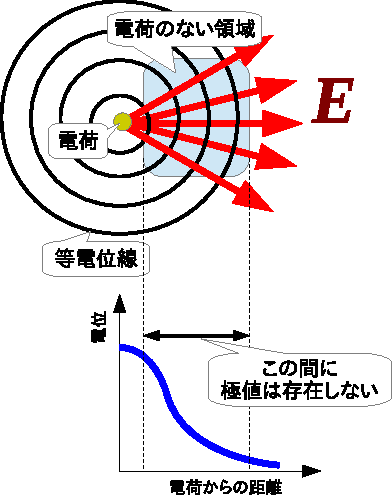
\includegraphics[keepaspectratio, width=6cm,height=7.74cm,clip]{StaticEF_Char1.pdf}
                        \caption{電荷が存在しない領域では,電位は極値をとらない}
                        \label{fig:StaticEF_Char1}
                    \end{center}
                \end{figure}

        \subsubsection{特徴2}\label{subsubsec:char2}
            等電位の閉曲面内に,電荷が存在しない場合,その内部領域全体の電位は,
            閉曲面の電位に等しく,一定である.これも,背理法で説明する.

            閉曲面の内部の電位が一定でない,と仮定する.
            閉曲面が等電位であることから,閉曲面上には電荷は存在しないので,
            この閉曲面の内側に,極値
                \footnote{
                    極値: 極大値あるは極小値のどちらかを指す総称.
                }
            が存在するはずである.
            極値が存在するということは,上記の特徴1の対偶から,
            閉曲面内に電荷が存在するはずである.
                \footnote{
                    特徴1の論理をかいつまむと,「極値が存在しない,ならば,電荷が存在しない」
                    となる.この対偶は,「電荷が存在する,ならば,極値が存在する」である.
                    一般に,「A$\Rightarrow$B」が成立するとき,その対偶「$\lnot$ B $\Rightarrow\lnot$ A」も
                    同時に成立する.
                }.
            しかし,これは,電荷が存在しないという前提に矛盾する.この矛盾は,
            閉曲面内の電位が一定でないという仮定からの帰結である.
            以上から,本特徴2を示せた.
                \begin{figure}[hbt]
                    \begin{center}
                        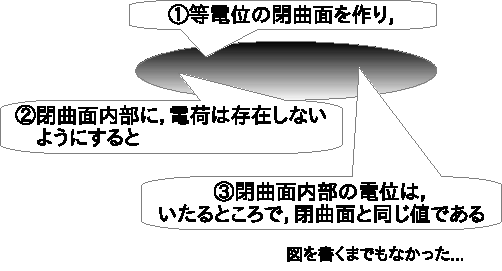
\includegraphics[keepaspectratio, width=6cm,height=5.4cm,clip]{StaticEF_Char2.pdf}
                        \caption{等電位の閉曲面内の電位(内部に電荷を含まず)}
                        \label{fig:StaticEF_Char2}
                    \end{center}
                \end{figure}


        \subsubsection{特徴3}\label{subsubsec:char3}
            任意の閉曲面において,閉曲面の内側の電荷分布と,閉曲面自体の電位が
            与えられれば,その領域内部の電位は,一意に決まる.

%       %==========================================================================
%       %  Subsection
%       %==========================================================================
        \subsection{アーンショーの定理}
        静電場中(ただし,電荷が存在しない領域に限る)では,荷電粒子は安定して存在できる
        位置がない.これを \textbf{アーンショーの定理} という
            \footnote{
                Samuel Earnshaw(1805--1888,イギリス):聖職者で数学者であった人らしい.
            }.
        この定理は,電場に限ったことではなく,磁場でも重力場でも成り立つ.
        距離に関する逆自乗の法則が成り立つならば,この定理が成立する.
                \begin{figure}[hbt]
                    \begin{center}
                        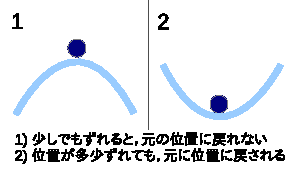
\includegraphics[keepaspectratio, width=5.11cm,height=2.91cm,clip]{Earnshow_000.pdf}
                        \caption{「安定な点」のイメージ}
                        \label{fig:Earnshow_000}
                    \end{center}
                \end{figure}

        実は,この定理は,すでに,上記の静電場の性質として,説明済みである.
        静電場に関するポアソン方程式からの帰結である.上記の性質をただ言い換えた
        だけだけど,この性質には「アーンショーの定理」とも呼ばれる別表現が
        あることを明記しておきたかった.


%   %==========================================================================
%   %  Section
%   %==========================================================================
    \section{導体}
        \begin{mycomment}
            導体といわれると,まず想像するのが,金属だろう.その他にも,
            炭素も有名だ.電解液(イオン溶液)も導体である
                \footnote{
                    ちなみに,純水は電気を通さない.水が電気を通すのは,
                    その中にイオンを含んでいる時のみであり,水道水が電気
                    を通すのも,それが完全な純水ではなく,不純物や塩素な
                    どのイオンを含んでいあるからである.
                }.
            なので,導体と言われても,想像される物質は色々と想像されてしまう.
            そこで,この章で考える導体の範囲に制限を与えることにしよう.
            ここで「導体」とよぶのは,金属や炭素などの個体で,その内部に
            自由電子をもつ物体を指すこととする.イオン溶液は確かに電気を
            通す導体ではあるが,除外する.
        \end{mycomment}

%   %==========================================================================
%   %  Subsection
%   %==========================================================================
    \subsection{導体とは}
        \subsubsection{導体,半導体,絶縁体}
        世の中には,様々な物体がある.石,木,水,葉,$\cdots$など,
        逐一例を上げていったのではきりがないほどだ.そして物体は,
        形,大きさ,硬さ,匂い,色,等,色々など性質をもっている.こういった性質の中で,
        電磁気学で特に興味がある性質に,"電気の通しやすさ" がある.
        電気の通しやすさは,物体を構成する物質そのものや,その構成に左右されるが,
        電磁気学ではそこまで細かいことは考えない
            \footnote{
                ここで学習する電磁気学は,現象論的なものである.
                物性などを含めて考えるときには,より詳細に,微視的
                な電磁気学を学習することも有用だが,内容が高度であるので,割愛する.
            }.
        目で見える範囲の物体を想像すれば十分である.
        とにかく,物体の塊を持ってきて,電気を通すか否かを判別するだけだ.
        物体の種類によって,電気の通しやすさは異なる.極端な例を上げると,
        ゴムは電気を通さないが,金属は電気を通す.様々な物体に対して,
        電気の通しやすさを調べると,それを順に並べることができる
            \footnote{
                電気の通しやすさを測定するには,対象となる物体の大きさを揃えたり,
                周囲の実験環境を揃えたりと,条件を一致させないといけない.
                ここでは,理想的に測ったと仮定しておこう.
            }.
        そうしてできた物体の順列で,電気を通しやすい部分に位置する物体のことを,
        \textbf{導体} という.反対に,電気を通しにくい部分に位置する物体のことは,
        \textbf{不導体} あるいは \textbf{絶縁体} という.
        簡単に言えば,導体とは電気を通しやすい物体のことである.
        また絶縁体は,電気を通しにくい物体のことを指す.

        ここで,"電気を通しやすい?" と表現した理由を説明しておこう
            \footnote{
                こんな回りくどい言い方をしないで,"電気を通す?" と表現したほうが,
                簡潔であると思われるかもしれないので.
            }.
        世の中には,様々な物体が存在するが,不思議な事に,「電気を(完全に)通さない
        物体」は存在しないのである.全ての物体が,電気を通すのである.ゴムなどの
        一般に電気を通さないとされる物体でも,詳細に測定すると,電気が流れることを
        確認できる.ただ,その流れる電気の量が非常に小さいので,電気を通していないと
        みなされるだけなのである.だから,電気を「通す/通さない」ではなく,
        「通しにくい/通しやすい」と書くべきなのである.

        とはいうものの,導体と絶縁体を明確に区別するような基準は存在しない.
        というか,定義すること困難なのである.導体と絶縁体とは,お互いに相対的な
        関係であり,状況によって変わりうるのである.例えば,紙は通常では絶縁体と
        して扱われるが,高電圧を紙にかける場合,電気を通すので,紙は導体として扱
        わないとならない.人間も,乾電池程度の電圧に対しては絶縁体だが,
        家庭用コンセントほどの電圧(100[V])に対しては導体となる
            \footnote{
                電化製品には,感電の恐れがあるという警告が大きく表示されているはず.
                特に,洗濯機において,アース(電気を体に通さないようにする仕組み)は絶対に
                欠かせない.
            }.
        では,導体と絶縁体の区別が全くできない程に曖昧かと
        言われれば,そうではない.\textbf{抵抗} という概念を使えば
            \footnote{
                オームの法則でお馴染みの,抵抗である.
            },
        ある程度区切りを入れることができる.抵抗による区切りも明確ではないが,抵抗は
        電気の通しやすさの1つの指標となる.
        抵抗は,電気物性を考えるときに重要な役割を果たす概念だが,電磁気学の
        理論的枠組を考える場合には,必要ではない
            \footnote{
                しかし,大切なので,後ほど解説をすることになるのだが$\cdots$.
            }.
        さしあたり,導体の例として金属をイメージすれば,十分である.また,
        絶縁体の例は,紙でも石でもゴムでもなんでもいい.
                \begin{figure}[hbt]
                    \begin{center}
                        \includegraphicslarge{DoutaiZetsuentai001.pdf}
                        \caption{導体と絶縁体}
                        \label{fig:DoutaiZetsuentai001}
                    \end{center}
                \end{figure}

        \subsubsection{理想的な導体}
            上記は,現実に存在する導体をイメージして記述した.
            これは,「物性物理学」よりの現実的な導体の説明である.
            しかし,多くの電磁気学の教科書で説明される「導体」は,
            少々異なる.
            電磁気学では,理論を考えやすくするために,理想化された導体を
            用いる.特に浸透している呼び方は無いようなので,
            このノートでは,\textbf{理想的な導体} と表現する.
            理想的な導体が,現実の導体と違う点を,いくつか上げておこう
                \footnote{
                    全部を上げることはできない.というか,思いつく限り上げたところで,
                    それで十分かどうかを判断することができないから.いや,
                    「理想的な導体」を理論的に整合性を保つように定義してやれば,
                    可能なのだけど,興味がない
                    (そんなことに時間をかけたくない,ってのが本音).
                }.
            \begin{myshadebox}{理想的な導体の性質}
                理想的な導体が持つ性質は,次の通り.
                \begin{enumerate}
                    \item 電荷には大きさがない(これは電磁気学全体をとおして同じ)
                    \item 正電荷と負電荷は導体中を自由に移動できる
                    \item 無限に多くの電荷をもっている(電荷の数に上限を与えない)
                    \item 導体中の電荷は,導体の外に出ることはできない
                    \item 連続分布している(原子レベルの不連続状態は考えない)
                \end{enumerate}
            \end{myshadebox}

            考えればいくらでも出てきそうだ
                \footnote{
                    教科書には,大抵の場合,こういった
                    ことは暗黙の了解として,明記されていない.紙面がもったいないからだろうか.
                    まあ,こんな約束なら,読めば簡単に悟れるから書くまでもないか.
                    書き始めるとキリがないし.
                }.
            この辺りで列挙を止めておこう.あとは,気が向いたら追記することにして,
            話をすめよう.

            上記の箇条書きに対して,補足しておきたい.理想的な導体を考える場合,
            それは原子で構成されていると考えてはいけない.確かに,正電荷と負電荷
            を持っているが,正電荷も導体内を自由に移動できるからだ.現実には,
            導体は原子で構成されていて,正電荷は動けない.正電荷も導体内を自由に移動
            できるという点が,はじめは違和感を感じるかもしれない.
                \begin{figure}[hbt]
                    \begin{center}
                        \includegraphicsdefault{risouteki_na_doutai000.pdf}
                        \caption{理想的な導体のイメージ}
                        \label{fig:DoutaiZetsuentai001}
                    \end{center}
                \end{figure}


%   %==========================================================================
%   %  Subsection
%   %==========================================================================
    \subsection{導体と電場の関係}
        \subsubsection{静電誘導}
        電場には,面白い性質がある.導体で囲まれた空間内部には電場は存在不可能
        なのである.導体はその内部に自由電子を含んでいる.この自由電子が,
        導体の外側の電場を打ち消すのである.
        自由電子は,導体中で移動できるため,導体の外側の電場から,
        クーロン力を受ける.自由電子は導体中に多数存在し,
        クーロン力に釣り合うように分布し,静止する.
        こうして静止した自由電子は,導体の外側の電場を完全に打ち消すように
        分布する.

        導体内部の自由電子が,外側の電場によって園分布が変わる現象を,
        \textbf{静電誘導} という.電子が電場に誘導されるイメージ.

        さらに言うと,電場は導体の表面で吸収され,導体中には浸透しない.
        導体内部が空洞だろうとなかろうと,導体の内部では一切電場は発生しない.
                \begin{figure}[hbt]
                    \begin{center}
                        \includegraphicsdefault{Doutai_to_Denba001.pdf}
                        \caption{静電誘導}
                        \label{fig:Doutai_to_Denba001}
                    \end{center}
                \end{figure}


        もちろん,電場を与えた
            \footnote{
                あるいは,電場の状態を変更しても同じこと.
            }
        直後は電荷の移動が起こるため,この間,導体内部にも電場が生じている.
        電荷がどのようにして導体中を移動するかも,興味のあるところだけど,
        ここでは,静電場内の現象を考えたいので,電荷の移動のことは後回し
        にしておこう.ここで考えたいことは,電荷の移動が完了したの,
        導体周辺に生じる静電場である.

        \subsubsection{静電遮蔽}
        上記の静電誘導の見方を変えると,
        導体の内部まで電場が突き抜けることはない,と言っても同じことだ.
        こうした立場からは,この現象を \textbf{静電遮蔽} という
            \footnote{
                あるいは,\textbf{静電シールド} とよばれれることもある.
            }.
        導体が電場を遮蔽するのだ.
                \begin{figure}[hbt]
                    \begin{center}
                        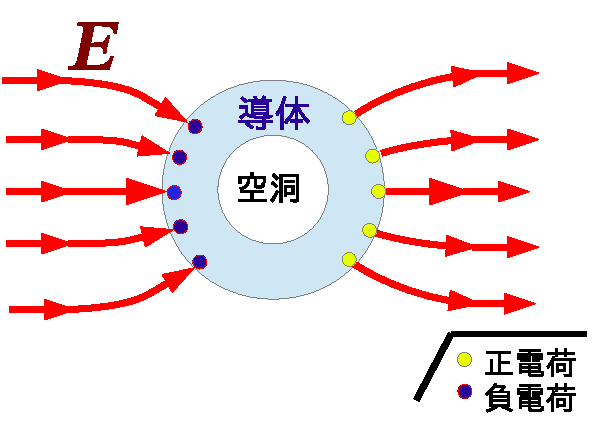
\includegraphics[keepaspectratio, width=6cm,height=4.2cm,clip]{Doutai_to_Denba000.pdf}
                        \caption{静電遮蔽}
                        \label{fig:Doutai_to_Denba000}
                    \end{center}
                \end{figure}

        電場の影響を極力少なくした実験を行う場合,この静電遮蔽が有効である.
        導体に完全に囲まれていれば,その中には電場は侵入してこないのだ.

        \begin{memo}{導体内部に電場は生じない}
            背理法を使って説明しよう(エネルギー保存則との矛盾をつかう).
            もし導体中に電場が発生すると仮定する.
            この時,導体内部の自由電子が,静電誘導を受け移動が始まる.
            しかし,これはエネルギー保存則に反する.なぜなら,
            エネルギーを与えていないにもかかわらず(電場はエネルギーではない),
            電流が生じるはずがないからだ.

            というか,そもそも,導体である条件の1つに,数え切らないくらいの
            自由電子をもっているという性質が要請されていて,電子は電場を吸収する
            のであるから,導体内部に電場が発生しないことは,導体の定義から直接的に
            示されるとも考えられる.
        \end{memo}

        \subsubsection{電場と導体表面}
        電場が導体の表面で吸収される場合,電場は導体表面に直交する.
        導体の形状がどんなに複雑でも,電場は表面に直角に交わる.
                \begin{figure}[hbt]
                    \begin{center}
                        \includegraphicsdefault{Doutai_to_Denba002.pdf}
                        \caption{電場は導体表面に直交する}
                        \label{fig:Doutai_to_Denba002}
                    \end{center}
                \end{figure}

        斜めに交わることはない.もし,斜めに交わってしまうと,導体表面に平行な電場成分が発生する.
        しかし,これは,先に示した導体の性質「導体内部に電場は生じない」と反する.だから,
        道内の内部に電場が生じないように交わるには,直角に交わるしかないのだ.
                \begin{figure}[hbt]
                    \begin{center}
                        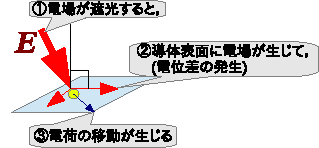
\includegraphics[keepaspectratio, width=6cm,height=2.7cm,clip]{Doutai_to_Denba003.pdf}
                        \caption{もし,電場が導体に直交しなかったら...}
                        \label{fig:Doutai_to_Denba003}
                    \end{center}
                \end{figure}

%   %==========================================================================
%   %  Subsection
%   %==========================================================================
    \subsection{導体と電位の関係}
    導体の表面は等電位面である.導体がどんな形をしていても,等電位面になる.
    電場が導体に垂直に交わることから,簡単に説明できる.
    \ref{subsec:toudeni_denba}節を参照.




%===================================================================================================
%  Chapter : 磁束密度に対するガウスの法則
%  説明    : 磁束密度に対するガウスの法則ビオ・サヴァールの法則から導く
%===================================================================================================
\chapter{磁束密度に対するガウスの法則}
%   %-----------------------------------------------------------------------------------------------
%   %  Input
%   %    File Name : PhysNote_EM_1st_GaussLowBF.tex
%   %-----------------------------------------------------------------------------------------------
        %   %==========================================================================
%   %  Section
%   %==========================================================================
    \section{ビオ$=$サバールの法則(復習)}
        \begin{mycomment}
            ビオ$=$サバールの法則についての詳細は,\ref{subsec:BiotSavart_Gene}節を参照.
            以下は,そこからの抜粋である.
        \end{mycomment}

        ビオ$=$サバールの法則は,磁束密度に関する法則である.
        \begin{myshadebox}{ビオ$=$サバールの法則(電流密度表示)}
            電流はその周囲に磁束密度を発生させる.その発生は以下の式に従う.
            \begin{align}
                \bB(\br)
                = \frac{\mu_{0}}{4\pi}
                    \int \frac{ \bi(\br')\times (\br-\br') }{ |\br-\br'|^{3} } \df V'.
            \end{align}
        \end{myshadebox}
        \begin{figure}[hbt]
            \begin{center}
                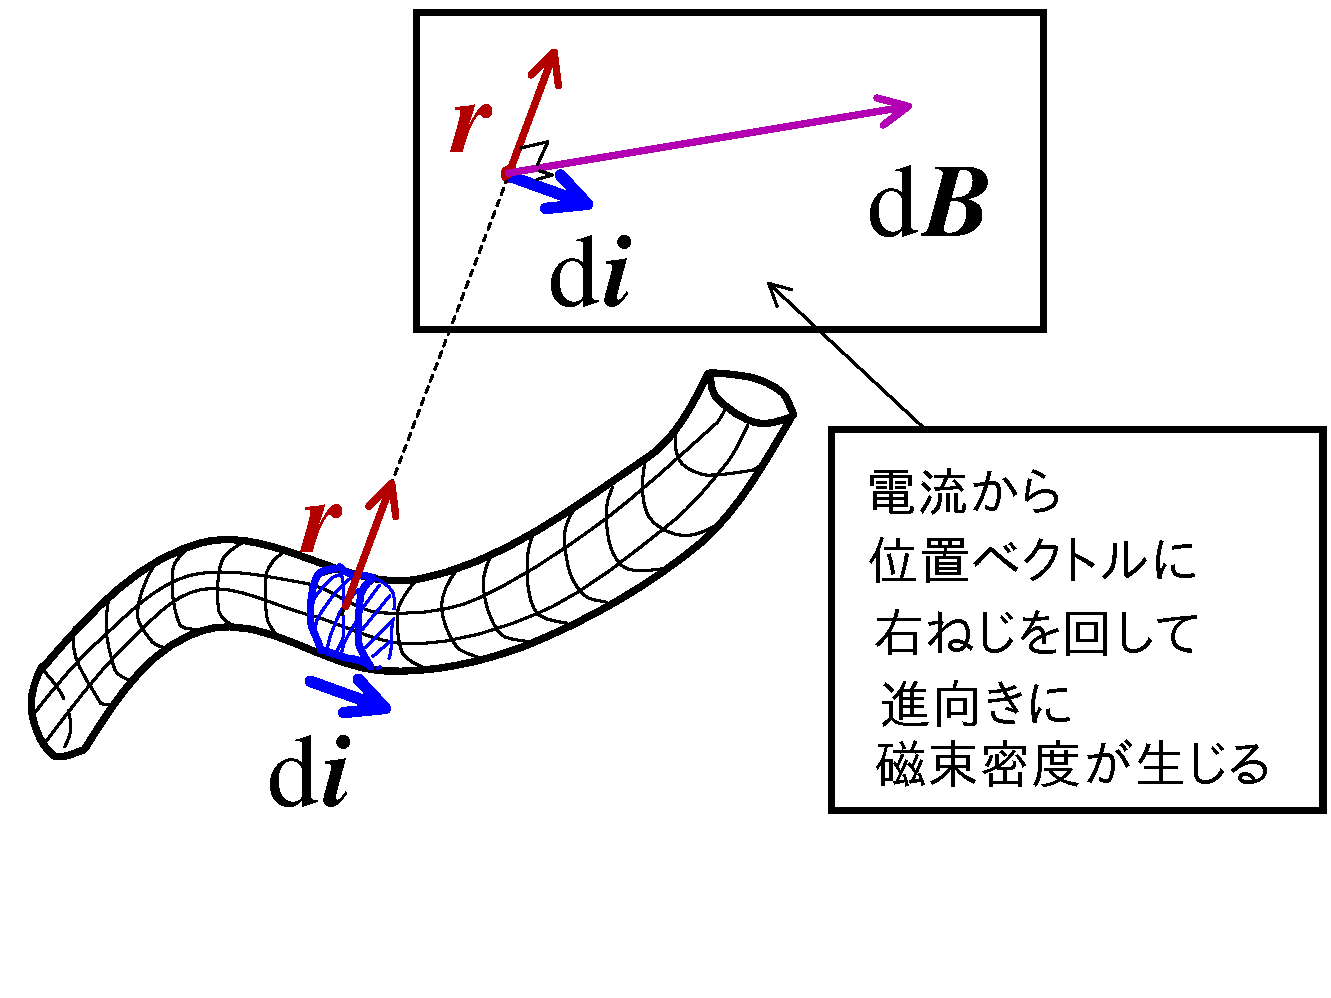
\includegraphics[keepaspectratio, width=7.2cm, height=5.79cm, clip]{biot_savart_1.pdf}
                \caption{ビオ$=$サバールの法則}
            \end{center}
        \end{figure}


%   %==========================================================================
%   %  Section
%   %==========================================================================
    \section{磁束密度に対するガウスの法則の導出}
%   %==========================================================================
%   %  Subsection
%   %==========================================================================
    \subsection{公式の確認}
        ビオ$=$サバールの法則から,磁束密度に対するガウスの法則を導出する
        手順を示す.まず,導出の際に以下のベクトル解析の公式を使用する.
            \begin{align}\label{eq:kousiki_kakunin}
                \dgrad \left( \frac{1}{r} \right) = - \frac{\br}{r^{3}}.  \\
                \drot (a\bX) = (\dgrad a) \times \bX + a(\drot \bX).
            \end{align}
        ただし,$r=\sqrt{x^{2}+y^{2}+z^{2}}$ である.また,$a$ は任意の
        スカラー関数であり,$\bX$ はベクトル関数である.

        \begin{memo}{公式の変形1}
            この公式を使うのだけど,このまま適用するわけではない.
            適用しやすいように,形を変えておこう.上段の式から見ていこう.
                \begin{equation*}
                    \dgrad \left( \frac{1}{r} \right) = - \frac{\br}{r^{3}}.
                \end{equation*}
            の $\br$ に注目する.任意の定ベクトル $\bC$ を考えて,$\br$ を
                \begin{equation*}
                    \br \rightarrow \br - \bC
                \end{equation*}
            と置き換えてやる.すると
                \begin{equation*}
                    \dgrad \left( \frac{1}{|\br - \bC|} \right)
                    =
                    - \frac{\br - \bC}{{|\br - \bC|}^{2}}
                \end{equation*}
            となる
        \footnote{
                    計算は合成微分を繰り返し.面倒だが,$x$ 成分の
                    計算だけでよいので,手で計算してほしい.
                    ここでは,記述が面倒なので,結果のみとする.
                }.
        \end{memo}

        \begin{memo}{公式の変形2}
            任意の定ベクトル $\bX$ に対して,
                \begin{equation*}
                    \drot \bX = \b0
                \end{equation*}
            が成立するとき,
                \begin{equation*}
                    \drot (a\bX) = (\dgrad a) \times \bX
                \end{equation*}
            が成り立つ.
        \end{memo}

%   %==========================================================================
%   %  Subsection
%   %==========================================================================
    \subsection{導出}
        ベクトル解析の公式 $\ddiv (\drot \bX) = 0$ を念頭に置き,
        ビオ$=$サバールの法則の式を変形していこう.

        まず,ビオ$=$サバールの式を書き下す.
            \begin{align}
                \bB(\br)
                =\frac{\mu_{0}}{4\pi}
                \int\frac{\bi(\br')\times
                (\br-\br')
                }{|\br-\br'|^{3}}\df V'.
            \end{align}
        この式の
            \begin{equation*}
                \frac{\br-\br'}{|\br-\br'|^{3}}
            \end{equation*}
        の部分の注目すると,公式
            \begin{equation*}
                \dgrad \left( \frac{1}{|\br - \bC|} \right)
                =
                - \frac{\br - \bC}{{|\br - \bC|}^{2}}
            \end{equation*}
        から
            \begin{align}
                \bB(\br)
                =\frac{\mu_{0}}{4\pi}
                    \int
                        \bi(\br')\times
                            \biggl\{
                                - \dgrad \left( \frac{1}{|\br - \br'} \right)
                            \biggr\}
                    \df V'.
            \end{align}
        さらに,公式($\bU$ は定ベクトル,$a$ はスカラー関数)
            \begin{align*}
                \drot (a\bU) &= (\dgrad a) \times \bU  \\
                             &= -\bU \times (\dgrad a)  \\
                             &= \bU \times (- \dgrad a)
            \end{align*}
        により,
            \begin{align*}
                \bB(\br)
                &=\frac{\mu_{0}}{4\pi}
                    \int
                        \bi(\br')\times
                            \biggl\{
                                - \dgrad \left( \frac{1}{|\br - \br'|} \right)
                            \biggr\}
                    \df V'
                 \\
                &= \int
                        \drot \left( \bi(\br') \frac{1}{|\br - \br'|} \right)
                    \df V'
                 \\
                &= \int
                        \drot \left(\frac{ \bi(\br') }{|\br - \br'|} \right)
                    \df V'.
            \end{align*}
        積分と微分の順番を変更して,
            \begin{align}
                \bB = \drot \int \left(\frac{ \bi(\br') }{|\br - \br'|} \right) \df V'.
            \end{align}

        ここで,次のようなベクトル関数を定義する.
            \begin{align}
                \bA(\br) := \int \frac{ \bi(\br') }{|\br - \br'|} \df V'.
            \end{align}
        これは後で \textbf{ベクトル$\cdot$ポテンシャル} と呼ばれる量と同じものである
            \footnote{
                ここでは,あくまでも形式的に導入するものであり,その正式な導入は後で行う.
            }.
        この $\bA(\br)$ をにより,ビオ$=$サバールの法則は以下のような形になる.
            \begin{align}
                \bB(\br) = \drot \bA(\br).
            \end{align}

        ここまで計算すれば,明らかだ.両辺に $\ddiv$ をとろう.
            \begin{align}
                \ddiv \bB(\br) &= \ddiv \left( \drot \bA(\br) \right). \notag \\
                \therefore \quad
                \ddiv \bB(\br) = 0.
            \end{align}
        この計算で,公式 $\ddiv (\drot \bX) = 0$ を使った.
        これは,磁束密度に対するガウスの法則に他ならない.

        以上の計算から,ビオ$=$サバールの法則に従って生じる磁束密度は,
        ガウスの法則 $\ddiv \bB(\br) = 0$ を満たすことが示された.


%   %==========================================================================
%   %  Subsection
%   %==========================================================================
    \subsection{まとめ}
        以上の結果をまとめよう.
                    \begin{myshadebox}{静磁束密度のガウスの法則(微分形)}
                        時間変化のない磁束密度に対する,局所的な
                        ガウスの法則は,以下の微分形の式により表される.
                        \begin{align}
                            \ddiv \bB =0.
                        \end{align}
                    \end{myshadebox}
                    \begin{myshadebox}{静磁束密度のガウスの法則(積分形)}
                        時間変化のない磁束密度に対する,大局的な
                        ガウスの法則は,以下の積分形の式により表される.
                        \begin{align}
                            \int_{S} \bB(\br) \cdot \bn(\br)\df S=0.
                        \end{align}
                    \end{myshadebox}

            磁束密度に対するガウスの法則は,
            電場に対するガウスの法則
            と同様に考えられる.
            磁束密度に対するガウスの法則
            を表す式を見てみると,
            『任意にとった閉曲面からの磁束密度の
            流出量を積分すると,その値は 0 に
            なる』
            ということ解釈できる.後で確認することではあるが,微分形のマクスウェル方程式によれば,
            磁束密度は,どの場所においても,発生 や 吸い込み がおきていないことがわかる.
            それゆえに,磁束密度の流出も生じないのである.


%   %==========================================================================
%   %  Section
%   %==========================================================================
    \section{法則の意味(図的イメージ)}


%===================================================================================================
%  Chapter : アンペール$=$マクスウェルの法則
%  説明    :
%           1.ビオ$=$サバールの法則から,定常電流のアンペールの法則を導く
%           2.電荷保存則とアンペールの法則の矛盾をのぞくべく,「変位電流」を導入する
%           3.変位電流をアンペールの法則に組み込み,アンペール$=$マクスウェルの法則を導く
%===================================================================================================
\chapter{アンペール$=$マクスウェルの法則}
%   %-----------------------------------------------------------------------------------------------
%   %  Input
%   %    File Name : PhysNote_EM_1st_AMLaw.tex
%   %-----------------------------------------------------------------------------------------------
        %   %==========================================================================
%   %  Section
%   %==========================================================================
    \section{アンペールの法則}
%   %==========================================================================
%   %  Subsection
%   %==========================================================================
    \subsection{エルステッドの実験}
        電流が生じている導体のそばに方位磁針をおくと,方位磁針は南北を示さなくなる.
        エルステッド
            \footnote{
                Hans Christian \O rsted ( 1777 - 1851, デンマーク  ):物理学者,科学者.
                太田光一の著した「電磁気学の基礎\I」には,"エールステズ" と片仮名表記されている.
            }
        はこの現象を発見した.その後,更に多くの実験が行われた.そして,アンペールによって,
        \textbf{アンペール力} (2つの電流の間に生じる力) が発見された.アンペール力 $\bF$ は,
        2つの電流を $I$, $I'$ とし,その間の距離を $l$ としたとき,
            \begin{align}
                \bF = k\frac{II'}{l}
            \end{align}
        で表される.$k$ は比例定数である.$k$ の具体的な数値は後で考えることになる
            \footnote{
                SI単位系において,電流の基本単位1[A] はアンペール力と利用し,定義される.
            }.
        2つの電流の間に,引力もしくは斥力(反発力)が発生するということである.
        2つの電流が同じ方向に向いていれば引力が働く.逆向きであれば,斥力が働く.

        原理を考えてみよう.
        電流の周りには磁束密度が生じる.また,電流とは電荷のいどうのことである.
        一方の電流が作る磁束密度の中を,他方の電流のもとである電荷が移動することになる.
        となれば,電荷は磁束密度中をある速度を持って移動することになるので,
        ローレンツ力を受けることになる.電荷というスケールで考えると,
        ローレンツ力を受けているのであるが,電流という大局的な視点で考えれば,
        アンペール力が働いているのである.アンペール力は原理的にはローレンツ力に
        起因するものと考えても良いが,時と場合によって,使い分けることが大事だ.
        例えば,実験や工学的な目的であればアンペール力を利用したほうが便利だし,
        現象を理論的に追求しようとした場合,ローレンツ力として考えたほうが
        一般性が高まることもあるだろう.

        話がそれたが,この節で言いたかったことは,電流の周囲には磁束密度が生じるという
        ことである.では,具体的には,どのような磁束密度が分布しているのだろうか.
        以下で考えていこう.


%   %==========================================================================
%   %  Subsection
%   %==========================================================================
    \subsection{ビオ$=$サバールの法則(復習)}
        \begin{mycomment}
            ビオ$=$サバールの法則についての詳細は,\ref{subsec:BiotSavart_Gene}節を参照.
            以下は,そこからの抜粋である.
        \end{mycomment}
            \begin{myshadebox}{ビオ$=$サバールの法則(電流密度表示)}
                電流はその周囲に磁束密度を発生させる.その発生は以下の
                式に従う.
                \begin{align}
                    \bB(\br)
                    =\frac{\mu_{0}}{4\pi}
                    \int\frac{\bi(\br')\times
                    (\br-\br')
                    }{|\br-\br'|^{3}}\df V'
                \end{align}
            \end{myshadebox}
            \begin{figure}[hbt]
                \begin{center}
                    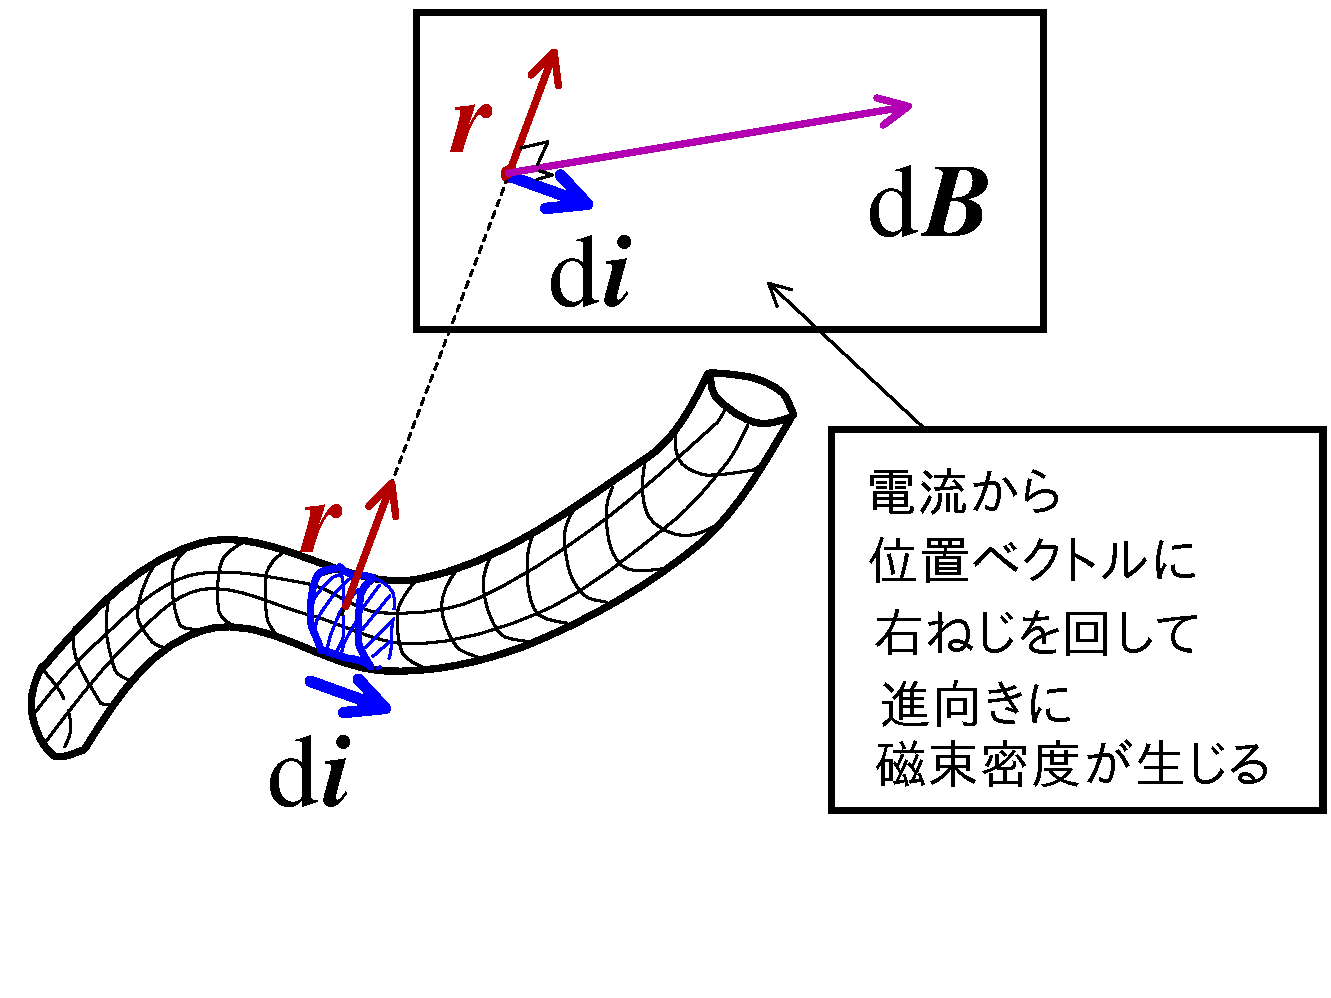
\includegraphics[keepaspectratio, width=7.2cm, height=5.79cm, clip]{biot_savart_1.pdf}
                    \caption{ビオ$=$サバールの法則}
                \end{center}
            \end{figure}

%   %==========================================================================
%   %  Subsection
%   %==========================================================================
    \subsection{アンペールの法則の導出}
%       %======================================================================
%       %  Subsection
%       %======================================================================
        \subsubsection{定常電流}
            ビオ$=$サバールの法則からアンペールの法則を
            導く.はじめに注意しておくと,ビオ$=$サバールの法則は時間変化しない電流
            についての法則である.このような電流を \textbf{定常電流} という.
            従って,以下に導くアンペールの法則も,定常電流を仮定していることになる.
          まず,定常電流を数式で表現しておく.

            電流とは電荷の集団の移動と定義される.電流が時間変化しないということは,
            電荷の移動の時間変化が一定であると考えられる.つまり,電荷密度の
            時間変化はないと解釈できる.ここで,
            電荷保存の法則をおもいだすと,
            \begin{align}
            \frac{\df }{\df t}\int_{\Omega_{S}} \rho(\br,t)\df V
            +\int_{S} \bi(\br,t)\cdot\textit{\textbf{n}}(\br)\df S=0
            \end{align}
            である.電荷密度 $\rho(\br,t)$ が一定の値をとることから,
            この式の第1項は 0 なる.つまり,この式に
            $\frac{\df }{\df t}\int_{\Omega_{S}} \rho(\br,t)\df V=0$ を
            代入して,
            \begin{align}
            \int_{S} \bi(\br,t)\cdot\textit{\textbf{n}}(\br)\df S=0
            \end{align}
            である.この式が定常電流を表現する式である.

%       %======================================================================
%       %  Subsection
%       %======================================================================
        \subsubsection{導出}
            定常電流であることを踏まえてアンペールの法則を導出する.ビオ$=$サバールの法則は
            式(\ref{Bior=savart'slow1})によって,
            \begin{align}
            \bB(\br)
            =\frac{\mu_{0}I}{4\pi}
             \int_{\Gamma}\frac{\bt(\br')\times
             (\br-\br')
            }{|\br-\br'|^{3}}\df s'
            \end{align}
            である.$\bt(\br')\df s'$ とまとめて,
            \begin{align}
            \bB(\br)
            =\frac{\mu_{0}I}{4\pi}
             \int_{\Gamma}\frac{\bt(\br')\df s'\times
             (\br-\br')
            }{|\br-\br'|^{3}}
            \end{align}
            である.
            この式の両辺を曲線 $\Gamma$ を内側に含む閉曲線 $l$ で線積分すると,
            \begin{align}
            &\oint_{l}\bB(\br)\cdot \bt(\br) \df l \notag \\
            &=\frac{\mu_{0}I}{4\pi}\oint_{l}
             \int_{\Gamma}\frac{\bt(\br')\df s'\times
             (\br-\br')
            }{|\br-\br'|^{3}}\cdot \bt^{\ast}(\br)
            \df l
            \end{align}
            とする.ここに,$\bt^{\ast}(\br)\df l$ は 閉曲線 $l$  単位
            接線ベクトル である.この式の右辺に ベクトル解析の公式
            \begin{align*}
            (\bL\times\bM)\cdot\bN
            =(\bN\times\bL)\cdot\bM
            \end{align*}
            を用いると,
            \begin{align}
            &\oint_{l}\bB(\br)\cdot \bt^{\ast}(\br) \df l \notag \\
            &=\frac{\mu_{0}I}{4\pi}\oint_{l}
             \int_{\Gamma}\frac{\bt^{\ast}(\br)\df l\times\bt(\br')\df s'
            }{|\br-\br'|^{3}}\cdot
            (\br-\br')
            \end{align}
            と変形できる.ここで,曲線 $\Gamma$ の単位接線方向ベクトル $\bt(\br')$ と
            閉曲線 $l$ の単位接線成分 $\bt^{\ast}(\br)$ との
            外積 $\bt(\br')\times\bt^{\ast}(\br)$ を
            \begin{align*}
            \textit{\textbf{n}}(\br')=\bt(\br')\times\bt^{\ast}(\br)
            \end{align*}
            とおく.また,$\df S_{l}=\df l\df s'$(「閉曲線 $l$ を縁とする面」という意味)とおく.すると,
            \begin{align}
            \oint_{l}\bB(\br)\cdot \bt^{\ast}(\br)\df l
            =\frac{\mu_{0}I}{4\pi}\oint_{l}
             \int_{S_{l}}\frac{\textit{\textbf{n}}(\br')\df S
            }{|\br-\br'|^{3}}\cdot
            (\br-\br')
            \end{align}
            と書ける.
            さらに曲線 $\Gamma$ が,閉曲線 $l$ の内側にあるので,公式
            \begin{align*}
            &\int_{S_{l}}\frac{\textit{\textbf{n}}(\br')\df S
            }{|\br-\br'|^{3}}\cdot
            (\br-\br') \\
            &=\int_{S_{l}}\frac{\textit{\textbf{n}}(\br')
            }{|\br-\br'|^{3}}\cdot
            (\br-\br')\df S=4\pi
            \end{align*}
            が成り立つ.従って,
            \begin{align}
            \oint_{l}\bB(\br)\cdot \bt^{\ast}(\br)\df l
            =\mu_{0}I
            \end{align}
            となる.この計算では,閉曲線 $l$ の単位接線ベクトルとして,$\bt^{\ast}(\br)$ を
            用いてきたが,ここで改めて,$\bt(\br)=\bt^{\ast}(\br)$ と
            書くことにしても混乱はないので,
            \begin{align}
            \oint_{l}\bB(\br)\cdot \bt(\br)\df l
            =\mu_{0}I
            \end{align}
            さらに,面 $S_{l}$ を流れる電流 を電流密度で表記すると,
            \begin{align}
            I=\int_{S_{l}} \bi(\br)\cdot\textit{\textbf{n}}(\br)\df S_{l}
            \end{align}
            と書けることから
            \footnote{
            この式の $S_{l}$ は閉曲面ではない.$S_{l}$ は
            閉曲線 $l$ を縁とした曲面である. → 電荷保存の法則で考えているのは
            閉曲面 $S$ であって,これとの違いに注意をする.
            },(電流は定常電流である.)
            \begin{align}
            \oint_{l}\bB(\br)\cdot \bt(\br)\df l
            =\mu_{0}\int_{S_{l}} \bi(\br)\cdot\textit{\textbf{n}}(\br)\df S_{l}
            \end{align}
            と表現できる.何度も確認するが,この式の $\bt(\br)$ は
            閉曲線 $l$ の単位接線ベクトルである.
                \begin{myshadebox}{アンペールの法則(積分形)}
                    電流の周囲には磁束密度が生じ,以下の式に従う.
                    \begin{align}
                        \oint_{l} \bB(\br)\cdot\bt(\br)\df l
                        =\mu_{0}\int_{S_{l}} \bi(\br)
                        \cdot\textit{\textbf{n}}(\br)\df S_{l}
                    \end{align}
                \end{myshadebox}

%   %==========================================================================
%   %  Subsection
%   %==========================================================================
    \subsection{法則の意味(図的イメージ)}
        言葉で言えば,「磁束密度 $\bB(\br)$ が
        存在する場所において,任意の閉曲線 $l$ を描き,この閉曲線 $l$ の接線方向に線積分すると,
        その値は閉曲線 $l$ の張る面 $S_{l}$ を貫く電流 $I$ の $\mu_{0}$ 倍に等しい」と言える.
        この式の解釈を簡単にいえば,『電流が磁束密度を生じさせる』ということである.
        つまり,(定常的な)磁束密度が存在するならば,その根源は電流である と言える.

        アンペールの法則を満たす磁束密度は一意に定まらない.そこで,静電場で考えた時と同じように
        磁束密度に対するガウスの法則を導入するのである.このガウスの法則によって,
        磁束密度を一意に決定できるようになる.

%   %==========================================================================
%   %  Section
%   %==========================================================================
    \section{アンペール$=$マクスウェルの法則}
    \begin{mycomment}
        アンペール$=$マクスウェルの法則とは,その記述から察しがつくと
        思うが,アンペールの法則にマクスウェルが改良を加えたものである.
        マクスウェルは,動電磁場を考える場合に,アンペールの法則が不完全
        であるとし,\textbf{変位電流} という新しい概念を導入した.変位電流とは
        なんなのか.マクスウェルはどのように修正したのか.その拡張された
        法則はどういったイメージなのか.この節で考えることにしよう.
    \end{mycomment}

%   %==========================================================================
%   %  Subsection
%   %==========================================================================
    \subsection{アンペールの法則と電荷保存則との矛盾}
        マクスウェルは,アンペールの法則に変位電流の項を加える修正を行った.
        なぜ,このような修正が行われたかというと,アンペールの法則が電荷保存則を
        満たさなかったからである.アンペールの法則は,電荷保存則と矛盾するのだ.
        この矛盾はどういったものなのかを,以下に示す.
            \begin{equation*}
                \drot \bB = \mu_{0}\bi.
            \end{equation*}
        両辺に発散($\ddiv$;divergence)をとってみる.
            \begin{equation*}
                \ddiv( \drot \bB ) = \ddiv ( \mu_{0}\bi ).
            \end{equation*}
        ここで,ベクトル解析の公式から,$\ddiv( \drot \bB ) = 0$ が成立している
            \footnote{
                (公式;定理)任意のベクトル $\bX$ にたいして,
                    \begin{equation*}
                        \ddiv( \drot \bX ) = 0
                    \end{equation*}
                が成立する.
            }.
        つまり,
            \begin{align*}
                \ddiv ( \mu_{0}\bi ) &= 0  \\
                \therefore \quad
                \ddiv \bi &= 0 \,,
                \quad(\because \mu_{0}\mbox{は定数})
            \end{align*}
        となる.ここで,式の見やすさの為に,右辺と左辺を入れ替えた.
        アンペールの法則を認める限り,この式が成立していなければ
        ならないのだけど,一方で,電荷保存則は
            \begin{equation*}
                \ddiv \bi = -\frac{\rd \rho}{\rd t}.
            \end{equation*}
        であり,右辺に関して,$\rd \rho/\rd t \neq 0$ である.
        明らかに,アンペールの法則と電荷保存則は矛盾してしまう.
        どちらが間違っているのだろうか.あるいは,両者とも間違って
        いるのだろうか.マクスウェルの出した答えは,アンペールの法則
        が不完全であるというもので,\textbf{変位電流} という概念を持ち出して,
        修正を加えた.現在では,変位電流の実在性は,電磁波の実験により確固たる
        ものとなっている.

%   %==========================================================================
%   %  Subsection
%   %==========================================================================
    \subsection{変位電流}
        マクスウェルが導入した変位電流とはどのようなものであり,また,
        変位電流の導入はアンペールの法則と電荷保存則の矛盾をどのように解決するか.
        これらを次に確認しよう.
        それには,
        電場に対するガウスの法則に,電荷密度 $\rho$ が現れていることに着目し,
        ここから電荷保存則の式に似せていくという,アプローチをとる.

        電場に対するガウスの法則によれば,
            \begin{align*}
                \ddiv \bE = \frac{1}{\varepsilon_{0}}\rho.
            \end{align*}
        両辺を時間 $t$ で微分する.
            \begin{align*}
                  \frac{\rd}{\rd t}\left(\ddiv \bE \right)
                = \frac{\rd }{\rd t}\left(\frac{1}{\varepsilon_{0}}\rho\right).
            \end{align*}
        ここで,空間に関する微分 $\ddiv$ と時間に関する微分 $\rd/\rd t$ の
        可換性を仮定して
            \footnote{
                時間微分と空間微分は可換であると,信じられている.
                ちなみに,ここに言う「可換」とは,演算の順番のことを言っている.
                つまり,時間微分と空間微分の計算順序を入れ替えてもよい,ということを
                主張している.要は,「空間に関するな微分演算」と「時間」に関する微分演算
                は独立していて,どちらを先に実行しようが,計算結果は変わらないということ.
            },
            \begin{equation*}
                  \ddiv \left(\frac{\rd \bE}{\rd t} \right)
                = \frac{1}{\varepsilon_{0}}\frac{\rd \rho}{\rd t}
            \end{equation*}
        となる.両辺に,$\varepsilon_{0}$ を掛けると,
            \begin{equation*}
                  \ddiv \left(\varepsilon_{0}\frac{\rd \bE}{\rd t} \right)
                = \frac{\rd \rho}{\rd t}.
            \end{equation*}
        最後に,両辺に$-1$をかける.
            \begin{equation*}
                  \ddiv \left( - \varepsilon_{0}\frac{\rd \bE}{\rd t} \right)
                = - \frac{\rd \rho}{\rd t}.
            \end{equation*}
        ここで,再度,電荷保存則の式を見てみよう.
            \begin{equation*}
                \ddiv \bi = -\frac{\rd \rho}{\rd t}.
            \end{equation*}

        電荷保存則と見比べてみると,$- \varepsilon_{0}(\rd \bE/\rd t)$ が
        電流密度と同じ働きをすることが見て取れる.しかし,この項は電流密度そ
        のものを表しているのではない事に注意しよう.
        この項 $\varepsilon_{0}(\rd \bE/\rd t)$ は \textbf{変位電流} とよばれる.

        電場の時間変化 $- \varepsilon_{0}(\rd \bE/\rd t)$ が,電流のように振る舞うように見える.
        考察している範囲に電荷密度が存在していなくとも,電場の時間変化が生じていれば,それを
        電流とみなして良いことを示唆していそうだ.
        アンペールの法則と電荷保存則との矛盾を解く鍵だと言っていい.
        実際にマクスウェルはこの項を持ち出して,アンペールの法則に手を加えて,矛盾を解消した.

%   %==========================================================================
%   %  Subsection
%   %==========================================================================
    \subsection{アンペール$=$マクスウェルの法則の導出}
        アンペール$=$マクスウェルの法則とは,前にも書いた通り,
        アンペールの法則に変位電流の考えを加えたものである.
        その方程式を先に書いてみれば,
        \begin{align}
            \drot \bB
                =   \mu_{0} \bi
                  + \varepsilon_{0} \mu_{0} \frac{\rd \bE}{\rd t}.
        \end{align}
        この方程式は,アンペールにより発見された \textbf{アンペールの法則} に,
        マクスウェルが修正を加えたもので,\textbf{アンペール$=$マクスウェルの法則} と
        よばれる.

        式の形を見るとは,単に,アンペールの法則の右辺に,
        変位電流を加えただけだ.しかし,電荷保存則との矛盾が解消されている.
        右辺第二項の $\varepsilon_{0} \mu_{0} (\rd \bE/\rd t)$ が
        あるため,$\ddiv \bi=0$ となっても,
                \begin{equation*}
            \drot \bB = \varepsilon_{0} \mu_{0} \frac{\rd \bE}{\rd t}.
                \end{equation*}
        となって,電荷保存則と矛盾はしない.
        この式を解釈すると,電場の時間変化が回転する磁場を発生させる,
        ということになる.

%   %==========================================================================
%   %  Subsection
%   %==========================================================================
    \subsection{法則の意味(図的イメージ)}

%   %==========================================================================
%   %  Section
%   %==========================================================================
    \section{静電容量}
%   %==========================================================================
%   %  Subsection
%   %==========================================================================
    \subsection{キャパシタンス}

    \begin{memo}{「キャパシタ」と「キャパシタンス」の違い}
    \end{memo}

%   %==========================================================================
%   %  Subsection
%   %==========================================================================
    \subsection{変位電流とキャパシタ}

%   %==========================================================================
%   %  Subsection
%   %==========================================================================
    \subsection{平行平板型のキャパシタ}

%   %==========================================================================
%   %  Section
%   %==========================================================================
    \section{電流のSI単位に基づく定義}
%   %==========================================================================
%   %  Subsection
%   %==========================================================================
    \subsection{直線電流が作る磁束密度}
        さて,今まで電流の単位として [A]=[C・s] を用いてきたが,
        先にも書いたように,これは現実の定義とは違うものである.
        SI単位系における基本単位は,電荷ではなく,電流が
        採用されている.

        今までの議論で電流を定義するための準備
        ができたので,そのための準備としてのこの項目と,次も項目で,
        電流の定義をし直すことにする.

        まず,定義の概略を示しておく.電流は電荷の移動によって生じる現象であるので,
        電流はローレンツ力を受ける.この電流に対するローレンツ力を人間が観測する
        するときは,導線が受ける力として観測される.
        その力は $\bF=\textit{\textbf{I}}\times \bB$ で表現できた.
        ここで,2つの平行な直線の導線を用意する.この2つの導線に同じ向きに電流を流すと,後に示すように,
        導線が互いに引き合う現象が生じる
        \footnote{
            電流を逆向きに流せば,導線同士は互いに反発しあう.
        }
        .この力によって電流を定義するのである.実際の力の大きさとしては $2\times 10^{-7}$ [N/m] が
        採用されている.
        導線同士が互いに引き合うのはローレンツ力によるものであり,これは
        一方の電流の作る磁束密度が,他方の電流(電荷)に及ぼすローレンツ力である.
        従って,1つの導線に流れる電流が作る磁束密度を計算する必要があり,
        ここではその計算をすることが目的である.そして,次の項目でここでの計算結果を
        利用して,電流を定義していこうと考える.

        直線電流が図\ref{fig:den_jisoku}のような磁束密度を作ることを確認する.
        1本の直線な導線を用意する.この導線に定常電流 $\textit{\textit{i}}$ を流し,
        この定常電流がその周囲に作る磁束密度を考える.
        アンペールの法則は
                    \begin{align}
                        \oint_{l} \bB(\br)\cdot\bt(\br)\df l
                        =\mu_{0}\int_{S_{l}} \bi(\br)
                        \cdot\textit{\textbf{n}}(\br)\df S_{l}
                    \end{align}
        のように書かれる.
            \begin{figure}[hbt]
                \begin{tabular}{cc}
                    \begin{minipage}{0.5\hsize}
                \begin{center}
                    \includegraphicsdouble{den_jisoku.pdf}
                    \caption{電流の作る磁束密度}
                    \label{fig:den_jisoku}
                \end{center}
                    \end{minipage}
                    \begin{minipage}{0.5\hsize}
                \begin{center}
                    \includegraphicsdouble{den_lorentz.pdf}
                    \caption{電荷の磁束密度から受けるローレンツ力}
                    \label{fig:den_lorentz}
                \end{center}
                    \end{minipage}
                \end{tabular}
            \end{figure}

        磁束密度の大きさは,ビオ$=$サバールの法則から,
        導線から等距離にある部分では等しくならないといけない.
        従って,直線の導線の任意の点を流れる電流が起こす,磁束密度の
        大きさが等しい部分をつないでいけば,その形は閉じた
        円になる.そして磁束密度の向きは電流の生じる方向に対して
        右回りである.図\ref{fig:den_lorentz}参照.これがわかれば,
        アンペールの法則の左辺;$\oint_{l} \bB(\br)\cdot\bt(\br)\df l$ の
        積分経路は,円にとればよいことがわかる.

        積分経路を円とすれば,その半径を $r$ とした場合に,
        磁束密度の強さは,以下のように計算される.

        アンペールの法則の左辺を計算すると,
            \begin{align*}
                \mbox{(左辺)}=\oint_{l} \bB(\br)\cdot\bt(\br)\df l
                      =\oint_{l}B\,\df l=B\oint_{l}\,\df l
            \end{align*}
        ここで,積分経路 $l$ は円であるので,$\oint_{l}\,\df l=2\pi r$ である.従って,
            \begin{align*}
                \mbox{(左辺)}=2\pi rB
            \end{align*}
        右辺;$\mu_{0}\int_{S_{l}} \bi(\br)\cdot\textit{\textbf{n}}(\br)\df S_{l}$ は,
        定常電流であるので,これは $\mu_{0}I$ と書ける.

        以上から
            \begin{align*}
                2\pi rB=\mu_{0}I
            \end{align*}
        すなわち,
            \begin{align}
                B=\frac{\mu_{0}I}{2\pi r}
            \end{align}
        である.

        \begin{memo}{積分経路を円にとる}
            なぜなら,円でない曲線経路を
            とったとしても,磁束密度の向きは円方向を向いているからである.
            下図参照.
                \begin{figure}[hbt]
                    \begin{center}
                        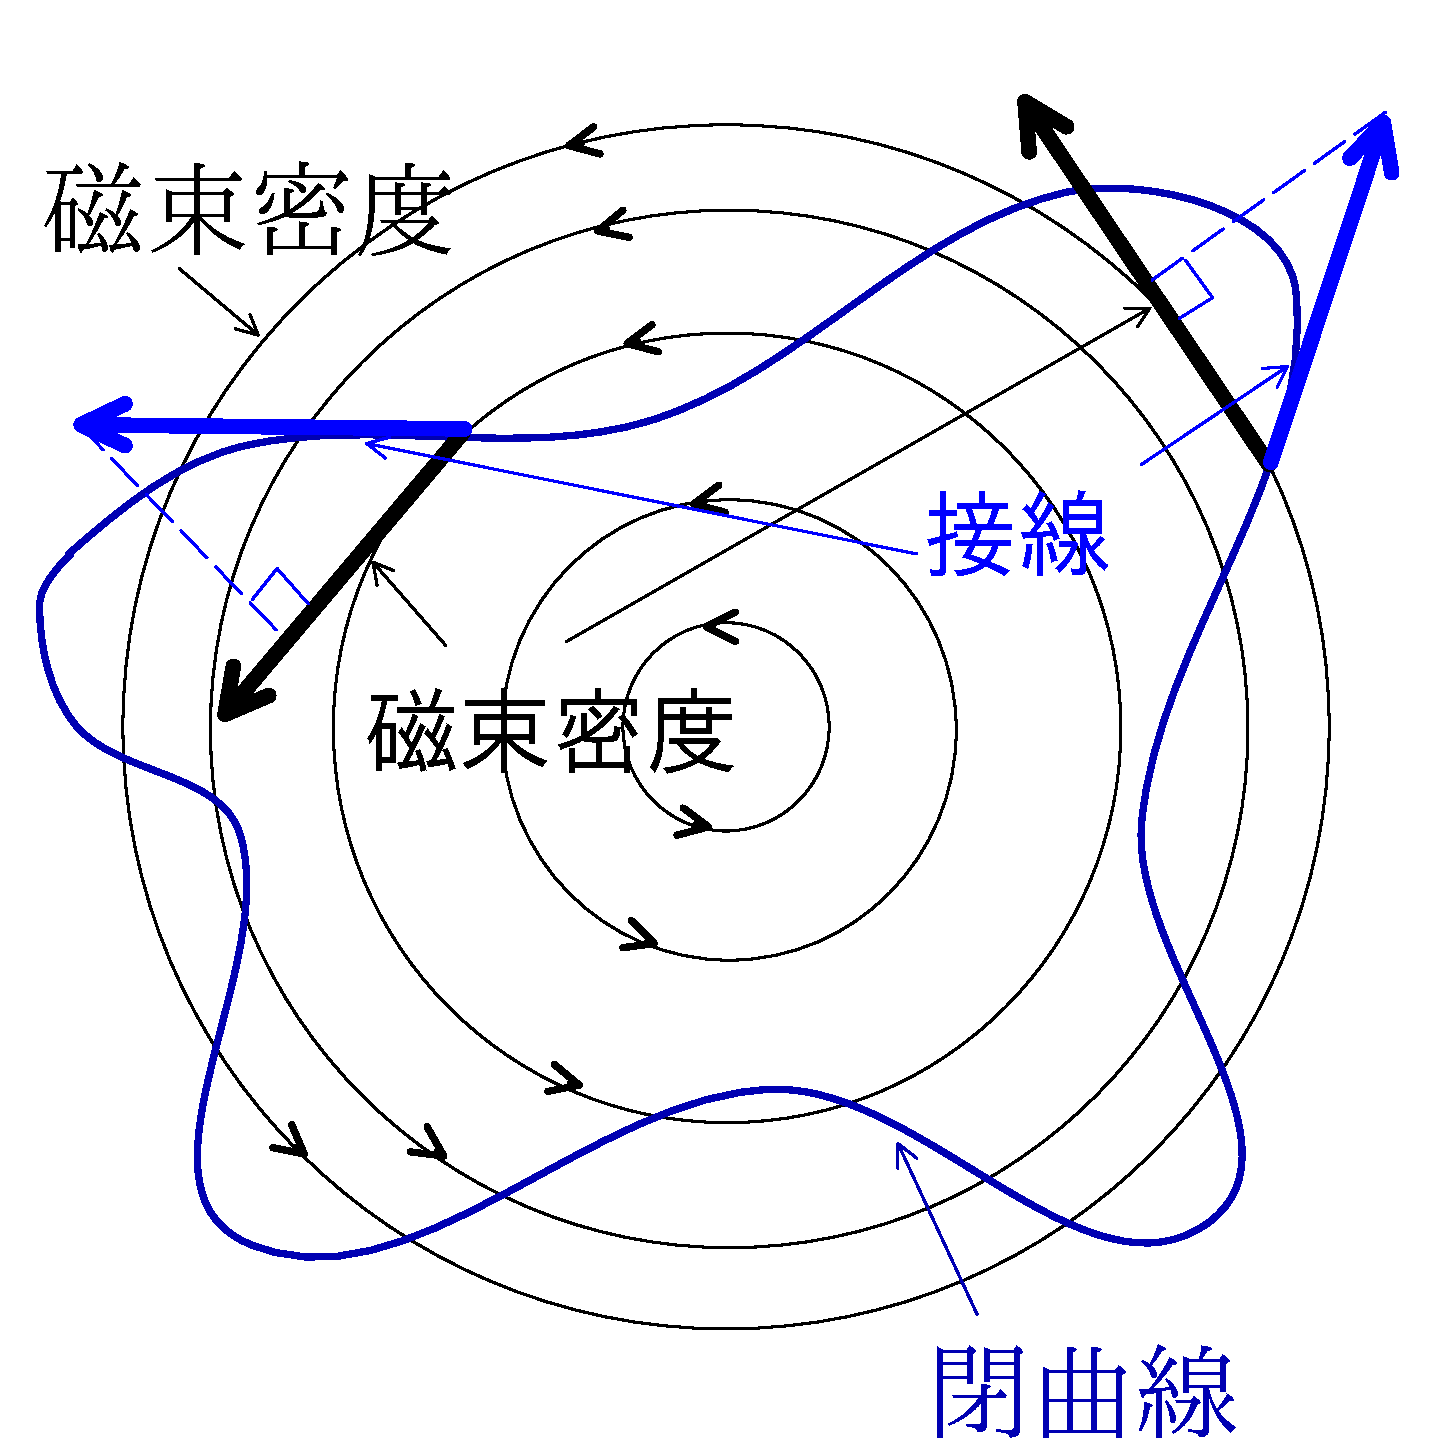
\includegraphics[keepaspectratio, width=6cm,height=6cm,clip]{dentei1.pdf}
                        \caption{閉曲線の取り方}
                        \label{fig:dentei1}
                    \end{center}
                \end{figure}

            図で示したように,曲線の接線と磁束密度の内積をとるので,
            接線の磁束密度に直角な方向成分は考察する必要がないのである.
            (考えたとしても,内積は0となるので意味がない.)
        \end{memo}

%   %==========================================================================
%   %  Subsection
%   %==========================================================================
    \subsection{電流が受ける力}
            電気量 $q$,速度 $\bv$  をもつ1つの電荷が受けるローレンツ力 $\bF$ をおもいだすと,
            \begin{align}
            \bF=q\bv\times\bB
            \end{align}
            であった.
            複数の電荷を考えれば,電荷密度という概念を導入して,
            \begin{align}
            \bF=\left(\int_\Omega \rho(\br)\df V\right)
            \langle\dot{\br}\rangle\times\bB
            \end{align}
            ここに,$\langle\dot{\br}\rangle$ は電荷のドリフト速度である.
            ドリフト速度というのは,複数の電荷の移動速度の平均である.
            そして,$Q:=\int_\Omega \rho(\br)\df V$ おくと,
            $\bF=Q
            \langle\dot{\br}\rangle\times\bB$ と書けて,
            $Q\langle\dot{\br}\rangle$ は電流を表現していると考えられるから,
            これを $\textit{\textbf{I}}$ おくことで($\textit{\textbf{I}}:= Q\langle\dot{\br}\rangle$),
            \begin{align}
            \bF=\textit{\textbf{I}}\times\bB
            \end{align}
            を得る.

%   %==========================================================================
%   %  Subsection
%   %==========================================================================
    \subsection{電流の定義(1[A]の定義)}\label{denryuuteigi}
            電磁気学ではSI単位系において,電流の単位が基本単位として
            採用されている.ここではその基本単位となる電流の1[A]を
            定義する.一つ前の項目\ref{dennryuunoukerutikara}で
            電流が受ける力は,導線の受ける力として現れることを確認し,
            その力は式(\ref{denruu_F})で表された.それをもう一度
            書き下せば,
                \begin{align}
                    \bF=\textit{\textbf{I}}\times \bB
                \end{align}
            である.
            \begin{figure}[hbt]
                    \begin{center}
                        \includegraphicsdefault{denryu_teigi.pdf}
                        \caption{電流の定義の説明図1}
                        \label{fig:denryu_teigi}
                    \end{center}
                \end{figure}

            2本の平行に並んだ導線を用意する.導線の名前をそれぞれ1,2とする.
            この2本の導線に定常電流を流す.それら2つの定常電流を
            それぞれ $\textit{\textit{i}}_{A}$,$\textit{\textit{i}}_{B}$ と
            する.この内の一方の導線に流れる電流が作る磁束密度を考える.
            どちらでもよいが $\textit{\textit{i}}_{1}$ の作る磁束密度を考える.
            アンペールの法則より,
                \begin{align*}
                    \oint_{l} \bB(\br)\cdot\bt(\br)\df l
                    =\mu_{0}\int_{S_{l}} \bi_{1}(\br)
                    \cdot\textit{\textbf{n}}(\br)\df S_{l}
                \end{align*}
            これは前項目で計算計算したように,
                \begin{align*}
                    B=\frac{\mu_{0}I_{1}}{2\pi r}
                \end{align*}
            である.従って,他方の導線に与える力は,
            (電流と磁束密度のなす角は $\pi/2$ であることに注意して)
                \begin{align*}
                    F=I_{2}B\sin\frac{\pi}{2}=I_{2}B
                \end{align*}
            従って,$B=\mu_{0}I_{1}/2\pi r$ を代入すれば.
                \begin{align}
                F=\frac{\mu_{0}I_{1}I_{2}}{2\pi r}
                \end{align}
            である.
            この式を用いて1[A]の電流を定義する.図\ref{fig:AARA}に描いたように,
            重さ $2\times10^{-7}$[N] のおもりを,同線の片方につるす.
                \begin{figure}[hbt]
                    \begin{center}
                        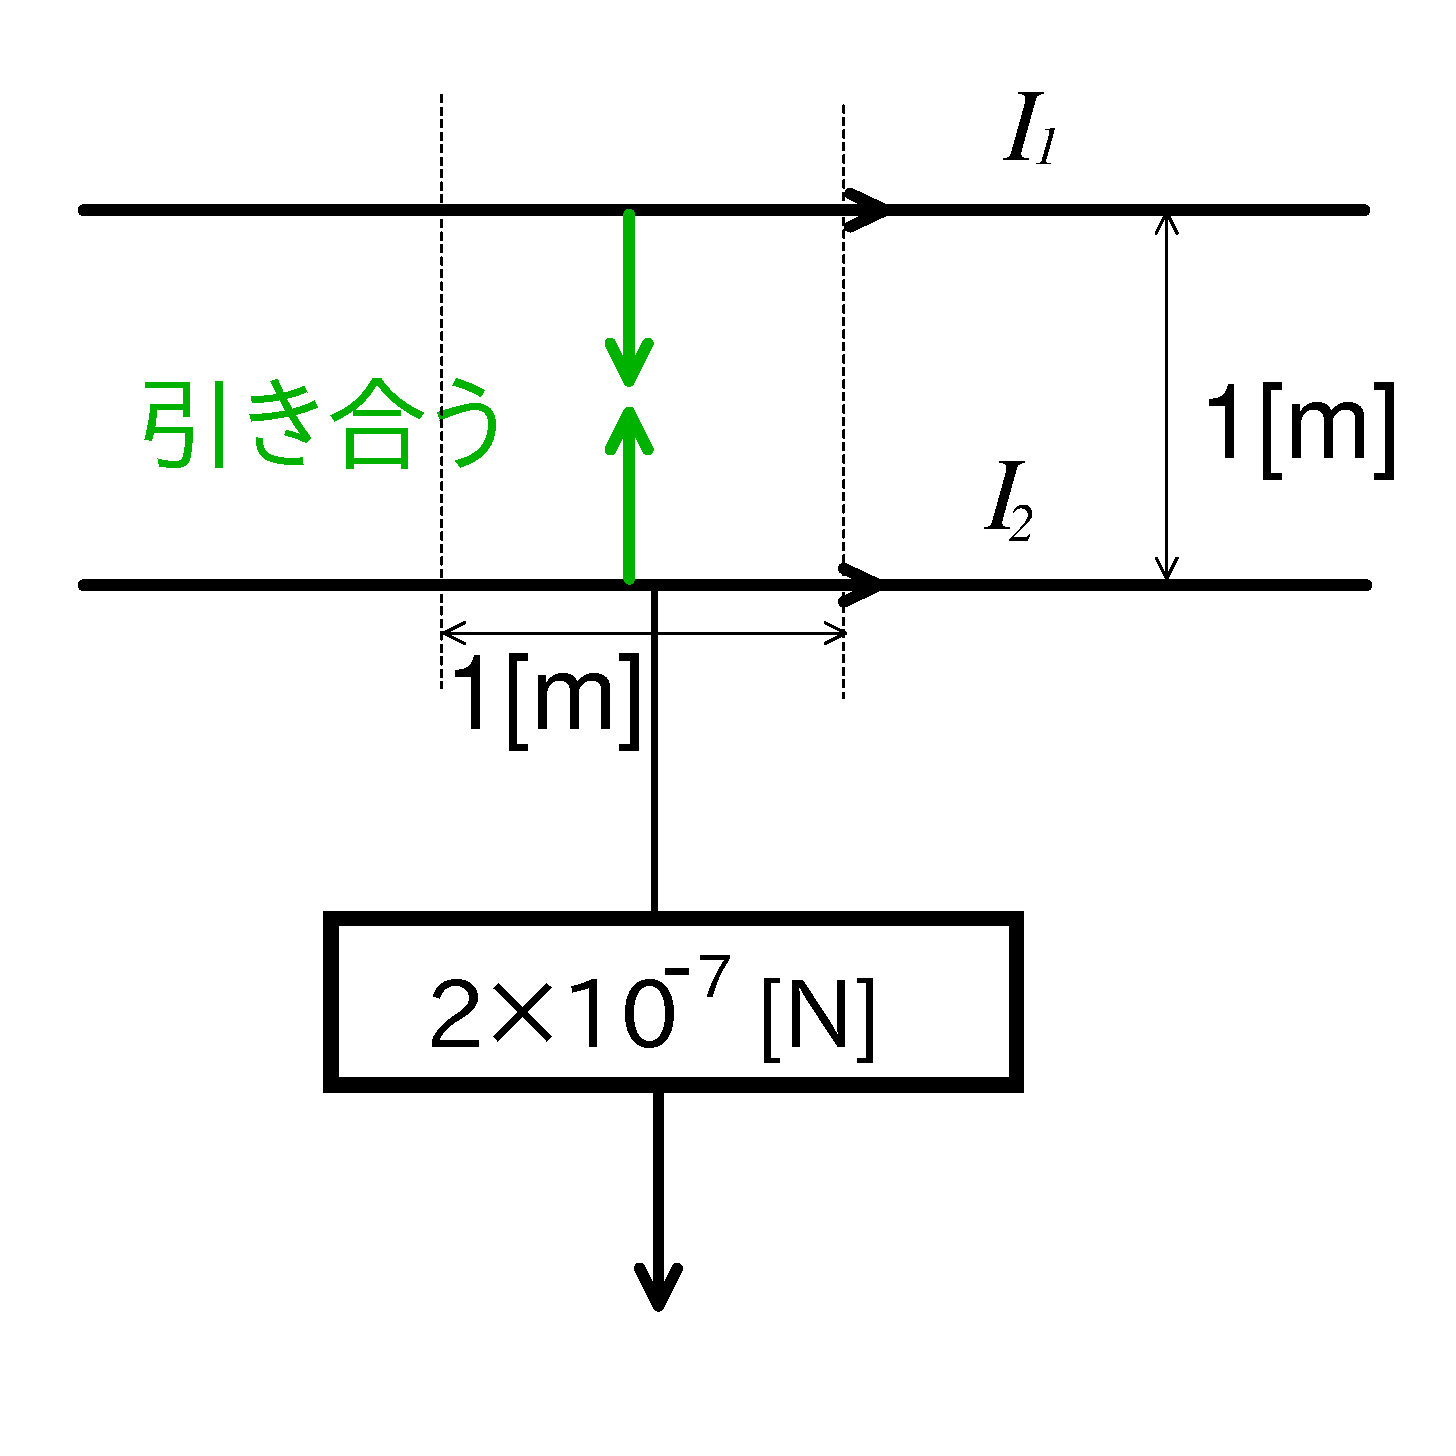
\includegraphics[keepaspectratio, width=5cm,height=4.5cm,clip]{AARA.pdf}
                        \caption{電流の定義の説明図2}
                        \label{fig:AARA}
                    \end{center}
                \end{figure}

            このとき,各導線には同じ方向に電流が流れているとする.
            導線間の距離は1[m]としている.
            この状態で,釣り合いが取れたとき,1[A]の電流が流れていると
            定義するのである.

            以上のことを形式的にまとめておこう.
                \begin{myshadebox}{電流1[A]の定義}
                    1[m]の間隔をおいた
                    2本の平行導線に電流を流して,
                    この導線に働く力が単位長さ(1[m])当たり $2\times10^{-7}$[N] の
                    力が働くとき,
                    この時に流れる電流を1[A]
                    と定義する.
                \end{myshadebox}


%===================================================================================================
%  Chapter : ファラデーの電磁誘導の法則
%  説明    :
%           1.ビオ$=$サバールの法則から,定常電流のアンペールの法則を導く
%           2.電荷保存則とアンペールの法則の矛盾をのぞくべく,「変位電流」を導入する
%           3.変位電流をアンペールの法則に組み込み,アンペール$=$マクスウェルの法則を導く
%===================================================================================================
\chapter{ファラデーの電磁誘導の法則}
%   %-----------------------------------------------------------------------------------------------
%   %  Input
%   %    File Name : PhysNote_EM_1st_EInduction.tex
%   %-----------------------------------------------------------------------------------------------
        %   %==========================================================================
%   %  Section
%   %==========================================================================
    \section{ファラデーの実験}
%   %==========================================================================
%   %  Subsection
%   %==========================================================================
    \subsection{起電力}
        「起電力」とは電流を発生させるためのエネルギー源である.
        具体的には 電池 と考えてよい.とにかく,電流を発生させる
        ものである.実際は,電流は電荷の移動であるので,従って,
        「起電力」とは電荷を動かすものである.電荷を動かすものと
        いえば,電場である.すなわち,起電力とは電場を導体内に発
        生させるエネルギー源であると言える.エネルギーと仕事の関
        係から,起電力は「導体内において,単位電荷を周させる仕事
        」と考えられる.従って,起電力を $V_{l}$ と書くと,(回路
        として閉ループ $l$ を想定するために,このような添え字を
        つけた.)
            \begin{align}
                V_{l}=\oint_{l} \bE(\br,t)\cdot\bt(\br,t) \,\df l
            \end{align}
        なる関係式を得ることができる.以後,\textbf{起電力} とは
        この $V_{l}$ のこという.


%   %==========================================================================
%   %  Subsection
%   %==========================================================================
    \subsection{磁束}
        イメージを先に書くと,「磁束蜜度の束」である.
        これは以下のように表現される.磁束密度を
        閉ループ $l$ を縁とする面 $S_{l}$ で面積分して,
            \begin{align}
                \Phi_{l}=\int_{S_{l}} \bB(\br,t)
                \cdot\textit{\textbf{n}}(\br,t) \,\df S_{l}
            \end{align}
        である.この $\Phi_l{}$ を \textbf{磁束} という.
            \begin{figure}[hbt]
                \begin{center}
                    \includegraphicsdefault{jisoku_image.pdf}
                    \caption{磁束のイメージ}
                    \label{fig:jisoku_image}
                \end{center}
            \end{figure}

%   %==========================================================================
%   %  Subsection
%   %==========================================================================
    \subsection{電磁誘導の法則}
            前にもビオ$=$サバールの法則の部分で書いたが,エルステッドは電流が生じるとそ
            の周りには磁束密度ができることを発見した
                \footnote{
                    電流を流している導線の近くに,方位磁針をいくつか置いてみると,
                    方位磁針は電流の作る磁束密度の方向に振れる.
                }.
            この現象はビオ$=$サバールの法則によって数学的に表現され,さらに,
            アンペールの法則と磁束密度に対するガウスの法則に形を変えている.

            ファラデーは電流が磁束密度を作るのならば,その逆作用として,磁束密度の
            中に置いた回路に電流が生じるのではないかと考えた.その実験の中で,彼
            は磁束密度の時間変化が電場を発生させることを発見した.そして,ノイマン
                \footnote{
                    Frantz Ernst Neumann:(1798 - 1895, ドイツの物理学者,鉱物学者)
                }
            は,この電磁誘導の法則を次のように定式化した.\\
                \begin{center}
                    \begin{itembox}[l]{\textbf{ファラデーの電磁誘導の法則}}
                        閉曲線 $l$ が張る曲面 $S_{l}$ を貫く磁束 $\Phi_{l}$ が時間変化すると,
                        この閉路 $l$ に起電力 $V_{l}$ が生じる.
                        この起電力 $V_{l}$ の大きさは,磁束 $\Phi_{l}$ の
                        時間変化率$\rd \Phi_{l}/\rd t$ に比例する.
                        また,起電力 $V_{l}$ の向きは,
                        この起電力によって閉路 $l$ に電流が生じるときに,
                        この電流が作る磁束がはじめの
                        磁束の変化を打ち消すような向きである.
                        起電力の向きに関すること
                        は \textbf{レンツの法則} とよばれる.
                        磁束 $\Phi_{l}$ の時間変化による閉路 $l$ 内に
                        生じる起電力 $V_{l}$ を,\textbf{誘導起電力} という.
                        ファラデーの電磁誘導の法則は,次式によって表される.
                        \begin{align}\label{denjiyudo}
                        V_{l}=-\frac{\rd \Phi_{l}}{\rd t}
                        \end{align}
                        誘導起電力によって回路に電流が生じるときに,
                        この電流が作る磁束がはじめの磁束の変化のきを正の向きとした.
                    \end{itembox}
                \end{center}

%   %==========================================================================
%   %  Subsection
%   %==========================================================================
    \subsection{法則の意味(図的イメージ)}
                電磁誘導の最も直感的なイメージを図\ref{fig:denjiyuudou},\ref{fig:denjiyuudou3}に示す
                    \footnote{図\ref{fig:denjiyuudou3}は
                        \url{http://vanity-worth.com/nature-law/lenz-1.htm}より(2008.08.24現在).
                    }.
                磁石が振動することによって,その磁石から生じている磁束が
                時間変化することになる.従って,この磁束密度の時間変化により,
                電場が生じることになる.もし,振動している磁石の周りに回路があるならば,
                回路の導線内には電場が生じ,従って起電力となる.
            \begin{figure}[hbt]
                    \begin{center}
                        \includegraphicsdefault{dennjiyuudou.pdf}
                        \caption{電磁誘導1-1}
                        \label{fig:denjiyuudou}
                    \end{center}
            \end{figure}
            \begin{figure}[hbt]
                    \begin{center}
                        \includegraphicsdefault{dennjiyuudou3.pdf}
                        \caption{電磁誘導1-2}
                        \label{fig:denjiyuudou3}
                    \end{center}
            \end{figure}

            電磁誘導の法則を別のイメージで考えてみる.原理は同じだが,次の例は
            とても面白い現象が得られる.

            コイルに電流を流すと磁束密度が生じることは,アンペールの法則から説明される.
            そこで,互いに近くに置かれた
            コイルを2つ用意し,片方(コイル1)にスイッチと電源を接続して,もう一方(コイル2)には
            何も接続しないようにする.図\ref{fig:denjiyuudou2}参照.

            まず初めの状態として,コイル1が電源に接続されスイッチが切れいている状態にする.
            このときはコイル1に電流が流れて得ておらず,従って,コイル1には磁束密度は
            生じていない.この状態からスイッチを入れてコイル1に電流を流してみると,
            この電流によってコイル1に電流が生じる.この電流は磁束密度を発生させる.
            つまり,コイル1の周りに「磁束密度の変化」があったことになる.
            ファラデーの電磁誘導の法則は,磁束密度の変化が回転する電場を生じさせるという
            ものであったので,
            この磁束密度の変化がコイル2の部分においても生じているはずであり,
            従って,コイル2に回転する電場が生じるはずである.つまり,
            コイル2に電流が生じるのである(電源がつながれていないのにもかかわらず!!).
                \begin{figure}[hbt]
                    \begin{center}
                        \includegraphicsdefault{dennjiyuudou2.pdf}
                        \caption{電磁誘導2}
                        \label{fig:denjiyuudou2}
                    \end{center}
                \end{figure}

            電磁誘導の法則(\ref{denjiyudo})を 電場 と 磁束密度 を用いて
            表現すれば,起電力 と 磁束 の項目から,次のように表現できる.
                    \begin{myshadebox}\textbf{ファラデーの電磁誘導の法則}
                        \begin{align}
                        \oint_{l} \bE\cdot\bt \,\df l =-\frac{\rd}{\rd t}\int_{S_{l}} \bB \cdot\textit{\textbf{n}} \,\df S_{l}
                        \end{align}
                        ここに,$\bE:=\bE(\br,t)$,$\bt:=\bt(\br,t)$,$\bB:=\bB(\br,t)$,$\bn:=\textit{\textbf{n}}(\br,t)$ であり,
                        位置と時間の関数である.これらが時間依存している点が重要である.
                        時間依存していなければ右辺は定数となり,静電場の方程式となる
                            \footnote{
                                この意味で,ファラデーの電磁誘導の法則は,静電場の方程式の
                                時間依存的な拡張と見ることもできる.
                            }.
                    \end{myshadebox}

%   %==========================================================================
%   %  section
%   %==========================================================================
    \section{自己誘導 / 相互誘導}
%   %==========================================================================
%   %  Subsection
%   %==========================================================================
    \subsection{自己インダクタンス}
        アンペールの法則によると,磁束密度 $B$ は電流 $I$ に比例する.
        先に見たとおり,磁束 $\Phi$ は 磁束密度 $B$ に比例するので
            \footnote{
                そのように,磁束を定義したのであった.
            },
        当然,\textbf{磁束は電流に比例する}.
            \begin{equation*}
               \Phi \propto B \propto I.
            \end{equation*}
        従って,磁束 $\Phi$ と電流 $I$ の関係式は,
        比例定数を $L$ としたときに,
            \begin{equation*}
                \Phi = LI.
            \end{equation*}
        これを電磁誘導の法則 $V=-\df \Phi/\df t$ に代入すると,
            \begin{align}
                V=-\frac{\df \Phi}{\df t}
                 =-L\frac{\df I}{\df t}
            \end{align}
        となる.この定数 $L$ を \textbf{自己インダクタンス} とよぶ.

        物理的イメージを考えてみよう.アンペールの法則により,電流は
        その周囲に磁束密度を発生させる.一方で,電磁誘導の法則によれば,
        時間変化する磁束密度の周囲には,電場が生じ,電位差が発生する.
        とすると,電流が流れていなかった導線に,突然に電流が流れ始めると,
        その周囲に磁束密度が発生するのだが,この磁束密度は時間変化するものであるので,
        同時に電位差もその周囲に生まれることになる.当然,いま流れ始めた電流は
        この電位差の影響もうけることになる.電流自身がその周囲に電位差を作り出し,
        その電位差が自身に帰ってくるのである."自己"インダクタンスと表現されている
        のは,この現象に由来している.

        \begin{memo}{磁束は電流に比例する}
            以下のように,簡略表記すると,わかりやすい.
            一重巻きのコイルを想定してみればよい.
            積分形のアンペールの法則は
            \begin{equation*}
                \oint_{l} \bB(\br)\cdot\bt(\br)\df l
                =\mu_{0}\int_{S_{l}} \bi(\br)
                \cdot\textit{\textbf{n}}(\br)\df S_{l}
            \end{equation*}
            であるから,
            \begin{equation*}
                B = \oint_{l} \bB(\br)\cdot\bt(\br)\df l
            \end{equation*}
            \begin{equation*}
                I = \int_{S_{l}} \bi(\br)\cdot\textit{\textbf{n}}(\br)\df S_{l}
            \end{equation*}
            と計算されたとき,
            \begin{equation*}
                B=\mu_{0}I.
            \end{equation*}
        \end{memo}

        \begin{memo}{ソレノイドが作る磁束密度}
            ソレノイド上の導線が作る磁束密度を考えよう.
            いま,ソレノイドを流れる電流 $I$ が定常状態であるとしたとき,アンペールの法則によって
            1回巻きの場合
            \begin{equation*}
                \oint_{l}B\,\df l =\mu_{0}I
            \end{equation*}
            である.$l$ はアンペールの法則に依れば任意の閉曲線
            であるから,ここでは図\ref{fig:sorenoido22}のように閉曲線をとってみる.閉曲線ABCDで,
            辺AB,辺CDの方向には,電流と平行な向きであるので,磁束密度は現れない.
            また,閉曲線ABCDの辺BCの部分には磁束密度は存在しない.なぜなら,この辺BCの部分は磁束密度が
            存在しない無限遠方と同じ空間でなければならないからである.つまり,
            磁束はソレノイドの内部だけに存在することになる.
            \begin{equation*}
            \oint_{l}B\,\df l=Bl
            \end{equation*}
            と計算されるから,
            \begin{align}
                Bl=\mu_{0} I
            \end{align}
            $N$ 回巻きの場合は,これを $N$ 倍すればよく,
            \begin{align}\label{sorenoidoB}
                Bl=N\mu_{0} I \\ \notag
                \therefore\quad B=\frac{N\mu_{0} I}{l}
            \end{align}
            この式(\ref{sorenoidoB})がソレノイド状のコイルに流れる電流がつくる磁束密度である.従って,
            この磁束密度を磁束 $\Phi$ に代入すると,
                \begin{align}
                    \Phi_{l}=BS=\frac{N^{2}S\mu_{0} I}{l}
                \end{align}
            である.ちなみに,この計算では巻き数 $N$ をコイルの総巻き数として計算しているが,
            単位長さあたりの巻き数 $n$ により表現すれば,$n=N/l$ から,$N=nl$ と書き換えて,
                \begin{equation*}
                    \Phi = \frac{(nl)^{2}S\mu_{0} I}{l} = \mu_{0}n^{2}lSI
                \end{equation*}
              となる.
                \begin{figure}[hbt]
                        \begin{center}
                                \includegraphicsdefault{sorenoido11.pdf}
                                \label{fig:sorenoido11}
                                \caption{ソレノイド(外観)}
                        \end{center}
                \end{figure}
                \begin{figure}[hbt]
                        \begin{center}
                                \includegraphicsdefault{sorenoido22.pdf}
                                \caption{ソレノイド(内部)}
                                \label{fig:sorenoido22}
                        \end{center}
                \end{figure}
        \end{memo}

    \begin{memo}{「インダクタ」と「インダクタンス」の違い}
        インダクタとは,現実に存在するコイルのことを意味する.
        インダクタンスと表現した場合には,理論上の比例定数のことをいう.
        似た表現であり,話すときにも混同してしまうことも多々あるが,意味は違うことを
        覚えておこう.
    \end{memo}

%   %==========================================================================
%   %  Subsection
%   %==========================================================================
    \subsection{相互インダクタンス}


%   %==========================================================================
%   %  Subsection
%   %==========================================================================
    \subsection{結合定数}

%   %==========================================================================
%   %  Subsection
%   %==========================================================================
    \subsection{変圧器の原理}




%===================================================================================================
%  Part : 特殊相対性理論
%  説明 : 特殊相対性理論についての記述.
%===================================================================================================
    \part{特殊相対性理論}
%   %-----------------------------------------------------------------------------------------------
%   %  Input
%   %    File Name : PhysNote_SR.tex
%   %    説明      : 特殊相対性理論のトップファイル.
%   %-----------------------------------------------------------------------------------------------
        %%**************************************************************************************************
%%
%% File Name : PhysNote_SR.tex
%% 説明      : 特殊相対性理論のトップファイル.
%%
%%**************************************************************************************************
%===================================================================================================
%  Chapter : 電磁気学の不満な点
%  説明    : アインシュタインの論文に基づいて,ローレンツ力と電磁誘導に関する説明で,
%            相対性が成り立っていないように見受けられることを指摘する
%===================================================================================================
\chapter{電磁気学の不満な点}
%   %-----------------------------------------------------------------------------------------------
%   %  Input
%   %    File Name : PhysNote_EM_2nd_MsgFirst.tex
%   %    説明      : マクスウェル方程式を前提に話を進める上での,心構え.
%   %-----------------------------------------------------------------------------------------------
        %===================================================================================================
%  Chapter : 電磁気学の不満な点について
%  説明    : アインシュタインの論文に基づいて,ローレンツ力と電磁誘導に関する説明で,
%            相対性が成り立っていないように見受けられることを指摘する
%===================================================================================================
%   %==========================================================================
%   %  Section
%   %==========================================================================
    \section{導入}
    特殊相対性理論は,アインシュタインが1905年に書いた
    “Zur Elektrodynamik bewegter K\"{o}rper”
    (動いている物体の電気力学)によって,始まった
        \footnote{
            いや,アインシュタインによって,
            「物理学的に完全な形に整えられた」
            と言った方が正確だろう.特殊相対性理論
            と同等の議論は,アインシュタイン以前にも
            盛んに行われていたからだ.言い換えれば,アインシュタインの他にも,
            特殊相対性理論の内容と同じ理論的枠組に迫った人がいる,ということ
            にもなる.
        }.
    特殊相対性理論は,光の速度の不可思議な性質
        \footnote{
                これは \textbf{光速度不変の原理} とよばれる,光のもつ
                性質の1つである.光の速さは,1つの慣性系において,
                運動している物体から光を出そうが,静止している物体から
                光を出そうが,
                両者の光の速度は一定の値($c=3\times10^{8}$[m/s])をとる,
                というものである.
        }
    をスマートに解決する理論である,と言いたいところだが,そうではない.
    アインシュタインは,光速度不変の原理を認めることで,
    より多くの物理現象を説明できる理論を組み立
    てることができると,主張する.その理論が,
    特殊相対性理論である.この章では,特殊相対
    性理論を確認する.特殊相対性理論は,アインシュタイン
    の1905年の最初の論文で,ほぼ完成している.
    有名な,時間の遅れという現象,棒の収縮といったことは
    この論文に全て書かれている
        \footnote{
            エネルギーと質量の関係式 $E=mc^{2}$ は,
            この論文には書かれていない.
        }.
    岩波文庫から,内山龍雄訳の原論文があるので,これを参照しながら,
    特殊相対性理論を勉強していこう.教科書は別のものを使う.

%   %==========================================================================
%   %  Section
%   %==========================================================================
    \section{ローレンツ力}
        ローレンツ力について,復習しよう.ある空間に,電場 $\bE$ と,磁束密度 $\bB$ が
        生じていることが分かっているとしよう.
        このとき,この空間に,電気量 $q$ をもった点電荷を,初速度 $\bv$ を与えて
        放す.すると,この点電荷は,空間からローレンツ力 $\bF$ を受けることになる.
        このローレンツ力 $\bF$ は,
            \begin{align}
                \bF = q(\bE + \bv \times \bB)
            \end{align}
        と書き表される.

%   %==========================================================================
%   %  Section
%   %==========================================================================
    \section{電磁誘導}
        ファラデーの電磁誘導の法則によると,磁束密度 $\bB$ の時間変化が
        その周りに回転する電場 $\bE$ を作り出す.式で書けば,以下の通り.
            \begin{align}
                \drot \bE = - \frac{\rd \bB}{\rd t}.
            \end{align}


%   %==========================================================================
%   %  Section
%   %==========================================================================
    \section{ローレンツ力と電磁誘導}
    原論文
        \footnote{
            原論文とはいっても,もちろん,日本語訳されたものを参照している.
            私にドイツ語が読めるわけがない.英語もよく読めないのに.

            参考図書のリスト\cite{bib:refbook_rel_1}を参照.
        }
    の冒頭で,アインシュタインは次のような,
    電磁気学における矛盾点を指摘している.
    それは,ローレンツ力と電磁誘導に関するものであ
    る.

    まず,磁石
    と金属棒を用意する.はじめに,磁石を固定し,
    金属棒を磁石の近くで,くっつけることのない
    よう,揺らしてみよう.このとき,金属棒内の
    電子に「ローレンツ力」が働く.

    今度は,逆に,金属棒を固定し,磁石を金属棒の近くで,
    棒をくっつけることなく,振ってみよう.このと
    き,磁石の振動によって,金属棒周囲の磁場が変
    動する.この磁場の変動は「電磁誘導」により,
    その周囲に電場を作り出す.この電場によって,
    金属棒に起電力が生じる.

    以上の2つの状況は,ともに電子の運動を引き起こす原因を
    説明するものである.そして,それらはともに,
    金属棒と磁石の“相対的な振動”によって,金属棒に
    起電力が生じるというものである.
    相対的な位置の変化が問題になるにもかかわらず,
    起電力発生の原因の説明が,視点を金属棒にするか,
    あるいは,磁石にするかによって,異なる.
    つまり,物理学的に,同じ状況であるのだけど,
    その現象の説明方法が異なっていまうのだ.
    これでは,納得のできないだろう.電磁気学に
    何らかの不備があると,感じてしまうこともあろう.

    そこでアインシュタインは,一歩後ろに引いて落ち着いて
    考察をする.そして,光速不変の原理と特殊相対性原理を
    基礎にし,「特殊相対性理論」を確立させる.
    この理論は,上のようなおかしな説明をせずに,
    起電力の発生を説明できる.そして,それだけにとどまらず,
    ニュートン力学を,より一般性の高い理論になるように,修正を加える.



%===================================================================================================
%  Chapter : 2つの基本原理
%  説明    : 特殊相対性理論,光速不変の原理を記述する
%===================================================================================================
\chapter{2つの基本原理}
%   %-----------------------------------------------------------------------------------------------
%   %  Input
%   %    File Name : PhysNote_SR_TwoPrinc.tex
%   %    説明      : 特殊相対性理論の土台となる,2つの基本原理,;
%   %                特殊相対性原理と光速不変の原理について,説明する.
%   %-----------------------------------------------------------------------------------------------
        %===================================================================================================
%  Chapter : 2つの基本原理
%  説明    : 特殊相対性原理と,光速不変の原理を説明する
%===================================================================================================
%   %==========================================================================
%   %  Section
%   %==========================================================================
    \section{特殊相対性原理}
%       %=======================================================================
%       % SubSection
%       %=======================================================================
        \subsection{物理法則と座標変換}
            物理現象を観測するのは,人間ひとりひとりである.
            当然ながら,ひとりの人間が同時に二つの視点に立って,
            同じ物理現象を観測することは不可能である
                \footnote{
                    「分身の術」なんてのは,考えない.
                }.

            しかし,二人の人間が,同時に,同じ物理現象を
            観測することは可能である.その場合,もちろん,
            二人の観測者の位置は異なっている.二人の観測者を
            A,Bとしよう.ある物理現象を,観測者Aの視点で見て,
            そして,物理法則を見出す.同様に,観測者Bの視点で見て,
            物理法則を見出す.観測者Aが発見した物理法則と,
            観測者Bが発見した物理法則に違いはあるだろうか.
            当然のことながら,両者の視点の違いによる差異はある.
            しかし,これは \textbf{座標変換} という操作で,両方の
            視点に行ったり来たりできる,ということを考えれば,その分の
            差異はなくなる(例えば,ガリレイ変換).
            そして,アインシュタインは,
            「観測者Aと観測者Bが発見する物理法則
            は,全く同じ形(全く同じ式)で,表されるはずだ」と言う.

        \begin{memo}{慣性系の存在 と ガリレイ変換(復習)}
            まず,慣性系が少なくとも1つ存在することを仮定する.
            実際には完全な慣性系を発見することは難しいだろうが
                \footnote{
                    ニュートンの万有引力の法則によれば,質量が存在
                    する場所では重力が存在するので,従って質量
                    付近では慣性系は存在しえない.しかし,ここ
                    ではこのようなことは無視して考える.気分が
                    スッキリしないだろうが,ここは一般相対性理
                    論への第一歩と考えて,この仮定を受け入れて
                    もらいたい.まあ,実際この仮定を受け入れて
                    ニュートン力学を考えてきたので(慣性の法則)
                    すんなり受け入れられるかもしれない.
                },
            ここではこれを理想化して考える.

            さて,慣性系が1つ存在するならば,ガリレイ変換によって,
            いくつもの慣性系が存在すると考えられる.それは簡単に
            示せる.最初に存在を認めた第1の慣性系を $S$ と表現す
            ることにし,この慣性系 $S$ を基準に取りこの速度を0と
            して考える.この基準慣性系 $S$ の位置座標を $\br$ と
            表現する.慣性系 $S$ に対して等速直線運動している慣
            性系を,ガリレイ変換によって考えることができて,この
            慣性系を $S'$ と表現する.慣性系 $S'$ の位置座標
            を $\br'$ と表現する.これら2つの座標系 $S$,$S'$ の
            位置座標には,ガリレイ変換により,
                \begin{align}\label{eq:gari1}
                    \br' =  \br+\bv t
                \end{align}
            という関係がある.ここに,$\bv$ は $S'$ の $S$ を基
            準とした相対速度であり,$t$ は時刻を表現する.この
            相対速度 $\bv$ を様々な具体的な速度で考えられるので,
            複数の慣性系を考えられるというわけである.

            次に,このガリレイ変換の逆変換を考える.逆変換とは慣
            性系 $S'$ から見た 基準慣性系 $S$ の運動を記述するこ
            とである.慣性系 $S'$ は基準慣性系 $S$ から見て相対
            速度 $\bv$ で運動しているので,慣性系 $S'$ から見れ
            ば基準慣性系 $S$ は $-\bv$ の相対速度で運動していな
            ければならない.従って,以下の式が導かれることになる.
                \begin{align}
                    \br =  \br'-\bv t.
                \end{align}
            逆変換における式操作については,“$\br$ と $\br'$ の
            場所を形式的に入れ替えて,速度を $-\bv$ と置き換える”
            ということをする.実際,この式は,式(\ref{eq:gari1})
            と矛盾していない(代数学的式変形で同じ式を導くことが
            できるということである).
            \end{memo}

%       %=======================================================================
%       % SubSection
%       %=======================================================================
        \subsection{特殊相対性原理}
            物理法則はどのような座標系からみても,同じ法則として表されるべきである.
            座標系が異なったら別の物理法則になってしまうのでは,物理法則とはいえない.
            この考え方を根本原理として掲げ,これを \textbf{特殊相対性原理} という.
            "特殊"とつくのは,特殊相対性理論の枠内での原理であることを明示するためである
                \footnote{
                    一般相対性理論ではこの原理は消えてなくなる.
                    「物理法則はどの座標系でも同じ」という \textbf{一般相対性原理} として
                    表現がより強く改められる.
                }.

            後で学習することだが,特殊相対性理論は慣性系での理論であり,一般的な加速度系
            では成立しない
                \footnote{
                    特殊な状況であれば,の加速度系で,特殊相対論を議論することは可能.
                }.

            特殊相対性原理はローレンツ変換
                \footnote{
                    ローレンツ変換とは,ニュートン力学で言うところこの,ガリレイ変換に相当する
                    座標変換である.速度が光速に近い物体を扱う場合には,物体の座標変換は
                    ガリレイ変換に従わず,ローレンツ変換に従うことが明白になる.
                    ガリレイ変換はローレンツ変換の特殊な場合に当たるもので,
                    物体の速度が光速に比べて非常に遅い場合に成り立つものである.
                    ローレンツ変換についても,このあとで学習することになる.
                }
            に対して不変であることを要請する原理であるともいえる.ローレンツ変換については
            このあとの記述する.


%   %==========================================================================
%   %  Section
%   %==========================================================================
    \section{光速不変の原理}
%       %=======================================================================
%       % SubSection
%       %=======================================================================
        \subsection{エーテル(電磁波と光)}
            電磁気学において,電場の波動方程式や磁束密度の波動方程式を
            導出したときに,電磁波が光速で伝わるということを確認した.
            これにより,\textbf{光は電磁波の一種である} ということが予
            言され,実際に実験によって確認されている
                \footnote{
                    このことについては電磁気学の章を参照.
                    また,量子力学によれば,光は光子(photon)
                    とよばれる“粒子”の一種でもあり,こ
                    れによって光は波動性と粒子性とをあわ
                    せもつものと考えられているが,このこ
                    とはここでは考えないことにする.
                }.

            さて,光が電磁波の一種であることが確認されたのであれば,光は
            波動であるということになるので,この光を伝える媒質が存在する
            と考えることは当然のことである
                \footnote{
                    例えば音は波の一種であり,その媒質は空気である.ま
                    た別の例を挙げれば,水面の波を考えられる.もちろん,
                    この水面波の媒質は水である.このように,波である以
                    上は何らかの媒質によってその変化が伝えられると考え
                    るのである.電磁波も波動現象であることが確認されて
                    いるので,電磁波を伝えるような媒質を見つけようとす
                    るのである.
                }.
            実際には,光を伝える媒質は存在しないことがアインシュタインによって
            宣言されるが,ここではこのような媒質を仮定して,この媒質の
            ことを \textbf{エーテル} ということにする.存在しないものに名前を
            つける理由は,歴史的にこれが存在すると考えられていたことも
            あるが,ここでは,エーテルの存在を否定するような実験を確認
            したいからということである.

%       %=======================================================================
%       % SubSection
%       %=======================================================================
        \subsection{マイケルソンとモーレイの実験}
            \begin{mycomment}
                ここでは,エーテルの存在を確認しようとす
                る実験である \textbf{マイケルソンとモーリーの実験} を
                見ていきたいと思う.これは光速度不変の原
                理を説明する1つの実証としてもみることがで
                きる.まず,光とは何かについての復習から
                始めていきたい.
            \end{mycomment}

            マイケルソン
                \footnote{
                    Albert Abraham Michelson (1852-1931,アメリカ)
                }
            と
            モーリー
                \footnote{
                    Edward Williams Morley(1838-1923,アメリカ)\;\;
                    この人物の片仮名表記は,「モーレー」,「モーリー」
                            等,複数存在している.
                }
            は光を伝える媒質であるエーテルの存在を実験によって確かめようとした.

            ここでは,その実験そのものを考えることはせず,
            この実験の要点を確認するだけにとどめる.
            図\ref{fig:MM_J}の装置が,
            エーテル内をABDに対して平行で等速度運動している
            とする.速度の向きはAからDへの向きとする.
                \begin{figure}[hbt]
                    \begin{center}
                        \includegraphicsdefault{MM_J.pdf}
                        \caption{マイケルソンとモーリーの実験1}
                        \label{fig:MM_J}
                    \end{center}
                \end{figure}

            この図\ref{fig:MM_J}のCとDの部分には
            ミラー(鏡)を置いてある.
            Cにあるミラーの傾きは進行方向に対して平行であり,
            Dにあるミラーの傾きは進行方向に対して垂直である.
            Bの部分には45°傾いている
            ハーフミラー
                \footnote{
                        光を半分反射し,
                                残りの半分をそのまま通すもの.
                }
            を置いてある.これによって,
            Aの部分にある光源から出た光は,
            Cへ向かうものとD向かうものに
            分割される.

            さて,この装置を用いて,Eへ到着する
            光を考えてみる.Eへ到着する光の経路は2つあり,
            それは A$\rightarrow$B$\rightarrow$C$\rightarrow$E の
            青色の線の経路(「青経路」ということにする)と,A$\rightarrow$D$\rightarrow$B$\rightarrow$E の
            赤色の線の経路(「赤経路」ということにする)である.すなわち,Eで観測される光は,
            青経路を通った光と
            赤経路を通った光が
            干渉したものになる.

            そこで,この干渉について
            式を使って考えてみる.
            光速を $c$ ,
            また装置の速度を $v$ と表すことにする.装置が速度 $v$ で運動しているので,
            実際の光の経路は以下の図\ref{fig:MM_J2}のようになる
                \footnote{
                    図\ref{fig:MM_J}は実験の内容をわかりやすくするためものであった.
                            従って,図\ref{fig:MM_J}は間違いであり,
                            より正しいのは図\ref{fig:MM_J2}である.
                }.
            但し注意してもらいたいのは,
            図\ref{fig:MM_J2}ではBD間が
            装置の速度の方向に縮まっているように見えてしまうが,
            装置は全体的に同じ速度で運動しているので,
            “BD間の距離が常に一定値 $L$ をとっている”
            ということである.
            \begin{figure}[hbt]
                \begin{center}
                    \includegraphicsdefault{MM_J2.pdf}
                    \caption{マイケルソンとモーリーの実験2}
                    \label{fig:MM_J2}
                \end{center}
            \end{figure}

            ここで大事なのは,この図\ref{fig:MM_J2}のB$\rightarrow$C$\rightarrow$B$'$を通る
            青径路の光と,B$\rightarrow$D$\rightarrow$B$'$を通る
            赤径路の光である.この 青径路を通った光 と 赤径路を通った光 が
            干渉すれば,エーテル
                \footnote{
                    光を伝える媒質のこと.
                }
            が存在するという実証になる.

            次に,この干渉を定量的に数式を用いて考えるために,
            2つの径路を通った光の時間差を計算してみよう.

            まず青径路の光を考える.
            より簡略化したものを以下の図\ref{fig:MM_J3}に描く.
                \begin{figure}[hbt]
                    \begin{center}
                        \includegraphicsdefault{MM_J3.pdf}
                        \caption{マイケルソンとモーリーの実験3}
                        \label{fig:MM_J3}
                    \end{center}
                \end{figure}

            光速 $c$ と装置の速度 $v$ によって,
            BからCへ向かう光の速度の成分は,$\sqrt{c^{2}-v^{2}}$ である.
            これを用いると,BC間の距離が $L$ であるとき,BからCに着くのに要する時間 $T$ を
            考えれば,$T=L/\sqrt{c^{2}-v^{2}}$ であるので,
            結局,BからB$'$へ着くまでにはその2倍の時間がかかっているはずである.
            この時間を $t_{1}$ (BからB$'$に着くのにかかる時間)とすれば,
                \begin{align}\label{eq:MM1}
                    t_{1}=\frac{2L}{\sqrt{c^{2}-v^{2}}}
                \end{align}
            であることがわかる.

            次に,赤径路を通る光について考える.まず,
            簡略した図を図\ref{fig:MM_J4}に描く.
                 \begin{figure}[hbt]
                    \begin{center}
                        \includegraphicsdefault{MM_J4.pdf}
                        \caption{マイケルソンとモーリーの実験4}
                        \label{fig:MM_J4}
                    \end{center}
                 \end{figure}

            反射前の光は,装置の速度$v$だけその速度が増して,
            このときの光の速さは $c+v$ である.従って,
            反射前の光がBからDに到達するのにかかる時間 $t_{\mbox{反射前}}$ は,
            BD間の距離が $L$ であるので,
                \begin{align}\label{eq:MM2}
                    t_{\mbox{反射前}}=\frac{L}{c+v}
                \end{align}
            である.


            光が反射するとき,図\ref{fig:MM_J4}では光の進む距離が短くなっているが,
            実際は装置全体が同じ速度で動いていることから,
            BD間の距離は変わることがない.このことに注意しながら,
            反射後の光について考える.
            光は反射後の光は装置の進行方向とは逆向きに進むので,
            このときの光の速さは $c-v$ である.従って,
            販社後の光がD$'$からB$'$に到達するのにかかる時間 $t_{\mbox{反射後}}$ は,
            B$'$D$'$間の距離が $L$ であるので,
                \begin{align}\label{eq:MM3}
                    t_{\mbox{反射後}}=\frac{L}{c-v}
                \end{align}
            である.

            従って,B$\rightarrow$D$\rightarrow$B$'$の赤径路
            を進む光が,この赤径路を往復するのにかかる時間 $t_{2}$ は,
            式(\ref{eq:MM2})の $t_{\mbox{反射前}}$ と式(\ref{eq:MM3})の $t_{\mbox{反射後}}$ の
            和であり,
                \begin{align*}
                    t_{2}   &= t_{\mbox{反射前}}+t_{\mbox{反射後}} \notag \\
                            &= \frac{L}{c+v} +\frac{L}{c-v} \notag \\
                            &= \frac{2cL}{c^{2}-v^{2}}.
                \end{align*}
            よって,
                \begin{align}\label{eq:MM4}
                    t_{2}&=\frac{2cL}{c^{2}-v^{2}}
                \end{align}
            となる.

            さて,以上で計算してきた結果をまとめてみる.青径路を
            往復するのにかかる時間 $t_{1}$ と赤径路を往復するの
            にかかる時間 $t_{2}$ の差をとると,
                \begin{align}\label{eq:MM_10}
                   t_{1}-t_{2}&=\frac{2L}{\sqrt{c^{2}-v^{2}}}-\frac{2cL}{c^{2}-v^{2}}\notag \\ \notag \\
                   &\cong\frac{2L}{c}\left( 1+\frac{v^{2}}{c^{2}}\right)
                   -\frac{2L}{c}\left( 1+\frac{v^{2}}{2c^{2}}\right) \notag \\
                   &=\frac{L}{c}\frac{v^{2}}{c^{2}}
                \end{align}
            となる.
            式変形の2段目の等号で,近似を用いていることに注意してほしい.
            すなわち,時間差が生じて,干渉縞がEに現れるのである.

            さて,理論上では,干渉縞が観測されるという予測が立てられた.
            ところが,この実験結果は“干渉縞が観測されない”ということである.
            すなわち,
                マイケルソンとモーリーの実験では \textbf{エーテルの存在を確認することができなかった} とい
            うことになる.残念なことに,理論的予測とその実証のための実験結果が矛盾してしまったことになる.

            次の項目で,この理論と実験結果との矛盾の解決の
            一例を考える.但し,完全な解決とはえないものだが$\cdots$.それでも確認する
            理由は,結論に出てくる式は大事であるということと,その変換式の名前(ローレンツ変換式)の由来を
            知るためである.


                \begin{memo}{式(\ref{eq:MM1})の解説}
                    距離 $X$,速度 $V$,時間 $T$ の関係は $X=VT$ であった.
                    ここでは,距離が $X=2L$,速度が $V=\sqrt{c^{2}-v^{2}}$,
                    時間が $T=t_{1}$ であったので,
                        \begin{align*}
                            2L=\sqrt{c^{2}-v^{2}}t_{1}
                        \end{align*}
                    が成立している.これを $t_{1}$ について
                    解くことで,式(\ref{eq:MM1})を得る.
                \end{memo}

                \begin{memo}{式(\ref{eq:MM_10})の近似式の解説}
                    この式変形に用いた近似は以下の近似公式によるものである.
                        \begin{align}
                            (1+x)^{n}=1+nx
                        \end{align}
                    ここに,$x$,$n$ は実数である.
                    まず,式(\ref{eq:MM_10})の式変形における
                    第1の等式の第1項は以下のように表現してもよい.
                    分母と分子をそれぞれ $c$ で割って,式を
                    近似式を適用できる形にしていく.
                        \begin{align*}
                            \frac{2L}{\sqrt{c^{2}-v^{2}}}
                            &=\frac{2L/c}{(\sqrt{c^{2}-v^{2}})/c} \notag \\
                            &=\frac{2L/c}{\sqrt{(c^{2}-v^{2})/c^{2}}} \notag \\
                            &=\frac{2L}{c}\frac{1}{\sqrt{1-\displaystyle\left(\frac{v}{c}\right) ^{2}}} \notag \\
                            &=\frac{2L}{c}\left( 1-\displaystyle\left(\frac{v}{c}\right)^{2} \right)^{-1/2}
                        \end{align*}
                    この式に先ほどの近似式を考慮すれば,
                        \begin{align*}
                            \frac{2L}{c}\left( 1-\displaystyle\left(\frac{v}{c}\right)^{2} \right)^{-1/2}\cong
                            \frac{2L}{c}\left( 1+\displaystyle\frac{1}{2}
                            \displaystyle\left(\frac{v}{c}\right)^{2} \right)
                        \end{align*}
                    を得る.これを式(\ref{eq:MM_10})の式変形における
                    第1の等式の第1項に考慮すると,上のような近似式を得る.
                \end{memo}


%       %=======================================================================
%       % SubSection
%       %=======================================================================
        \subsection{光速不変の原理}
            マイケルソンとモーリーの実験でも推察されるように,
            エーテルという物質は存在しないと考える方がよ
            いのである.これは \textbf{光の速さが,その光源もつ運動の速度にかかわらずに,
            一定の値 $c$ をとる}と解釈してもよい.
            これが \textbf{光速度不変の原理} である.
            このように考えれば,干渉縞が
            現れないのも当然のこととなる.

            アインシュタインはこの考えを,
            特殊相対性理論の論文で,宣言している
                \footnote{
                    ポアンカレも『科学の価値』で
                    この考えを提案している.
                }.

            しかし,光速不変の定理という言い方には
            少し注意が必要である.というもの,
            この光速度不変の原理は,
            慣性系で成り立つものだからである.
            つまり加速度をもった系では,もはやこの法則は
            成立しない.この問題は,
            一般相対性理論によって解決される.
            とにかく,光速度不変の原理は
            慣性系という特殊な状況でのみ成立し得る法則であるということだ.



            \textbf{光速度不変の原理} を以下に書き表す.
            \begin{myshadebox}{光速度不変の原理}
                    『1つの静止系を基準に取った場合,
                    いかなる光線も,それが静止している物体,
                    あるいは運動している物体のいずれから放射されてかには関係なく,
                    常に一定の速さ $c$ をもって伝播する.
                    』(アインシュタイン 著,内山 龍雄 訳,『相対性理論』より)
            \end{myshadebox}

            この光速度不変の原理で注意すべきことは,
            \textbf{観測者の速度が異なる場合,光速は一定値をとることを主張していない}ことである.
            例えば,二人の観測者が異なる速度で運動しているとしよう.この二人の観測者が,
            それぞれ同じ光源から発せられる光の速度を測定したとき,その値が $c$ で一致するとは,
            この光速度不変の原理は,主張しない.

            では,二人の観測者が異なる速度で運動している場合,それぞれ観測する光速は違うのだろうか.
            結論からいえば,観測者がどのような速度で運動していようとも,観測される光速 $c$ で一定値を
            とる,と言える.これを確認しておこう.

            二人の観測者が測定した光速を,それぞれ $c_{1}$,$c_{2}$ とする.$c_{1}$ も $c_{2}$ も
            一定の値であることから,
                \begin{equation*}
                    c_{1}=\phi(v) c_{2}
                \end{equation*}
            となる,$\phi(v) $ が存在するはずである
                \footnote{
                        例えば, $c_{1}=6$,$c_{2}=3$ の場合,$\phi(v)  =2$ である.
                }.
            ここに,$v$ は二人の相対速度であり,$\phi(v)$ の変数である.
            二人とも,同じ方向に進む光の速度を観測すれば,$\phi(v)$ は正の値をとる
            はずである.

            ところで,特殊相対性原理によれば,どんな慣性系でも物理法則は全く同じである.
            つまり,
                \begin{equation*}
                    c_{2}=\phi(-v)  c_{1}
                \end{equation*}
            も成立している.  速度が $-v$ となることに注意.この2式から,
                \begin{equation*}
                    c_{1}=\phi(v)  c_{2}=\phi(v) \, \{\phi(-v)  c_{1} \}
                \end{equation*}
                \begin{equation*}
                    \Leftrightarrow \quad \phi(v) \, \phi(-v)  = 1
                \end{equation*}
                \begin{equation*}
                    \therefore \quad \phi(v)  =1
                \end{equation*}
            となる.つまり,
                \begin{equation*}
                    c_{1}=c_{2}
                \end{equation*}
            である.従って,観測者がどのような速度で運動していようが,光速は
            一定の値をとることがわかる.その光速の値は,1つの慣性系で $c$ を
            示していることから,$c:= c_{1}=c_{2}$ である.再度注意しておくが,
            この結果は,光速度不変の原理が直接示しているのではなく,
            特殊相対性原理との論理的結果であるということである.
            観測者の速度にかかわらず,光速が一定値をとるということは,
            数学でいう定理のようなものである.
            \begin{figure}[hbt]
                \begin{center}
                    \includegraphicsdefault{RT_kousoku_ittti.pdf}
                    \caption{速度の異なる慣性系において,同一光源から生じる光の速度を測定}
                    \label{fig:RT_kousoku_ittti}
                \end{center}
            \end{figure}


%===================================================================================================
%  Chapter : 特殊相対論的な現象
%  説明    : 特殊相対性理論,光速不変の原理を記述する
%===================================================================================================
\chapter{特殊相対論的な現象}
%   %-----------------------------------------------------------------------------------------------
%   %  Input
%   %    File Name : PhysNote_SR_SRPheno.tex
%   %    説明      : 同時性の破滅,棒の収縮など
%   %-----------------------------------------------------------------------------------------------
        \section{特殊相対論的な現象}
\begin{mycomment}
この節では,特殊相対性原理と光速度不変の原理
によって起こる例を考える.最初に,
同時刻について考える.
その次に,Lorentz収縮と
時間の遅れを考える.
そして,
マイケルソンとモーリーの実験
矛盾を解決するローレンツ変換式
を,上の2つの基本原理だけによって
導出する.
\end{mycomment}


\subsection{同時刻}
\begin{mycomment}
光速度不変の原理によって,同時刻という従来のニュートン力学的な概念は,成り立たなくなって
しまうのである.そこで次に,同時刻の概念の考え直しをしたいと思う.
\end{mycomment}


同時刻については,
具体的に考えるとわかりやすい.例として,「2つの異なる場所より発せられる光が
“同時刻”に届く」とはどういうことかを考える.2つの光源の名前をそれぞれA,Bとする.
当たり前のことではあるが,\textbf{
光源Aと光源Bの光が観測点Oに“同時刻”に届くとは,
それぞれ光源から発せられた光が
時間差なく届くということである.}
さて,より詳しく考えるために,
以下のような状況を設定し,考察していこう.

まず理想的な
\footnote{
ここでいう「理想的」とは,
車輪の摩擦や空気抵抗,
燃料の増減による
質量の増加等の
現実性を全て仮想的に
排除したということである.
}
電車を想定し,この電車両端(前と後ろ)に光源を
取り付ける.前の光を
青にし,
後ろの光を赤にする.
そして,電車が
前の方向に等速度速度 $V$ をもって運動しているとする.
但し,この電車の速度は
光速 $c$ に比べて十分に小さいものとする(すなわち,$V\ll c$).
このとき,
光が電車の真中に到達する様子を
以下の2つの立場で考える.
まず第1に,
観測者がこの車両の真中で
この光の到達を観測するという立場で考える.そして
第2に,
これを電車の外で静止している別の観測者の
立場で考える.
この考察で,この両者の同時刻は異なってしまうことを
みることになる.

早速考える.第1の立場の状況は図\ref{fig:doujikoku1}のように描ける.
                \begin{figure}[hbt]
                    \begin{center}
                        \includegraphicsdefault{doujikoku1.pdf}
                        \caption{同時刻1(電車の中の観測者からの視点)}
                        \label{fig:doujikoku1}
                    \end{center}
                \end{figure}

この立場の観測者は,光源と同時に運動している.従って,
前から来る青い光 と 後ろから来る赤い光 は同時刻に
観測者の目に入ってくる.

では次に第2の立場,すなわち,電車の外で静止している
観測者からの視点で考える.この場合の状況は
図\ref{fig:doujikoku2}のように描ける.
\textbf{
光は,電車内の観測者が「“同時刻”に前後の
光源が発光した」と主張するように
光源を発光させているものとする.}
すなわち,第1の立場と同じ
状況を,電車外の静止した場所から
観測してみようということである.
実はこの仮定は同時刻を
考え直すのに大事になるので,
この仮定を覚えておくこと.
                \begin{figure}[hbt]
                    \begin{center}
                        \includegraphicsdefault{doujikoku2.pdf}
                        \caption{同時刻2(電車外の静止した観測者からの視点)}
                        \label{fig:doujikoku2}
                    \end{center}
                \end{figure}

この図で注意したいのは
“電車が動いても,光速は常に一定値 $c$ をとる”
ということである.
これは,光速度不変の原理による要請である.

この図を見ると,後ろから
発光した赤い光は電車の速度の方向に
進むだけ,
また他方では,前から発光した青い光は
電車の進行方向と逆向きに
進むので,
従って,
青い光が赤い光よりも先に
電車の真中に
到達することになる.
だから,
電車外で静止している
観測者には,赤と青の
光が同時に
電車の真中に
到達しない
と主張することになる.
これは,
光速が一定であるから,
電車が動けば,その電車の動いた分だけ
光が進むからである.


では,青い光と赤い光との
到達時刻の差は
どの程度だろうか.その時間差を考えることにする.
この電車の長さを $l$ とする.
このとき,光源Aまたは光源Bからの
電車の真中までの距離は,それぞれ $l/2$ である.
青い光についてまず考えると,青い光が電車の
真中までに要する時間を $t_{\mbox{青}}$ として,
青い光の進む距離 $X_{1}$ を考えると,
電車の速度が前の方向に $V$ であることを考慮し,
\begin{align}\label{eq:douji_1}
X_{1}=\frac{l}{2}-Vt_{\mbox{青}}
\end{align}
である.ところで,光速度不変の原理によって,
光の速度は光源のもつ速度に関係ないので,
\begin{align}\label{eq:douji_2}
X_{1}=ct_{\mbox{青}}
\end{align}
も成立しているはずである.従って,式(\ref{eq:douji_1}),式(\ref{eq:douji_2})から,
\begin{align}\label{eq:douji_3}
ct_{\mbox{青}}&=\frac{l}{2}-Vt_{\mbox{青}} \notag \\
\Leftrightarrow \quad
ct_{\mbox{青}}+Vt_{\mbox{青}}&=\frac{l}{2}\notag \\
\Leftrightarrow \quad
(c+V)t_{\mbox{青}}&=\frac{l}{2} \notag \\
\Leftrightarrow \quad
t_{\mbox{青}}&=\frac{l}{2(c+V)}
\end{align}
である.一方,赤い光について
も同様に考えると,光の進行方向が
お会い光と逆方向なだけなので,
\begin{align}\label{eq:douji_4}
t_{\mbox{赤}}=\frac{l}{2(c-V)}
\end{align}
計算される.
式(\ref{eq:douji_3})と式(\ref{eq:douji_4})を比較すると,
$l$,$c$,$V$ は全て定数であるから,
$t_{\mbox{赤}}$ が $t_{\mbox{青}}$ よりも大きいことがわかる.
すなわち,赤い光が電車の真中に到達する時刻は
青い光よりも遅れるということになる.どのくらい遅れるか
といえば,
\begin{align}\label{eq:douji_5}
t_{\mbox{赤}}-t_{\mbox{青}}&=\frac{l}{2(c-V)}-\frac{l}{2(c+V)}\notag \\ \notag \\
&=\frac{2l(c+V)-2l(c-V)}{2(c-V)\times 2(c+V)}\notag \\ \notag \\
&=\frac{2lc+2lV-2lc+2lV}{4(c-V)(c+V)}\notag \\ \notag \\
&=\frac{lV}{c^{2}-V^{2}}
\end{align}
である.

ここで最初の光の点灯時刻に関する
仮定を思い起こすと,
“光源の発光は電車内の観測者が
同時刻に発光したと主張する
ように光源を発光させている”
ということであった.
これはつまり,
\newline \newline
\textbf{主張1};「電車内の観測者にとって,
赤い光と青い光が
同時刻に到達したと
観測される」
\newline \newline
ということである.
しかし,
電車外の人間から見れば,
青い光が赤い光
よりも先に電車の真中に
到達していて,
つまり,電車外の人間は,
\newline \newline
\textbf{主張2};「
電車内の人間は同時刻に
赤い光と青い光を観測していない」
\newline \newline
と主張するのである.

主張1と主張2は明らかに矛盾している.
これは,「電車内の人間の同時刻の発光」と
「電車外の人間の同時刻の発光」が
全く別の見方であるということを示唆する.
そこで,同時刻の概念の
考え直しが必要になるのである.
この矛盾を解決するには次のように考えるとよい.

電車内の観測者が青い光と
赤い光が同時に発光したと主張しているということは,
電車内の人間にとって,
青い光と赤い光が時間差なく
届いたということである.
この仮定を前提としたここでの
考察で矛盾を生まないためには,
\textbf{電車外の静止した観測者にとって,
青い光と赤い光の発光時刻は
異なっている} と考えるのである.
すなわち,電車外の人にとっては,
赤い光が先に点灯し,
赤い光の点灯時刻より $lV/({c^{2}-V^{2}})$ の
時間間隔の後に青い光が点灯している
ように見えるのである.

電車内の観測者は
青い光と赤い光は
同時に点灯したと
主張し,
電車外の観測者は
青い光と赤い光は
異なった時刻に点灯
していると
主張する.
観測者によって,
その主張の内容が
異なっているが,
矛盾はしていない.
この両者の
主張の違いは,
それぞれの属する
慣性系が異なることに
依るものである.
今までの同時刻の概念は,
慣性系に依らないものであった.
しかし,光速度不変の原理を仮定ている今,
もはや従来の同時刻の概念は通用しない
ものであるということは,
以上の確認ではっきりと分かった.
つまり,\textbf{
同時刻の概念は
慣性系によって異なるものである} ということである.
ある慣性系では同時刻に起こる現象が,
別の慣性系では異なる時刻に起こっている現象である
ということを認めねばならない.






\subsection{ローレンツ変換式}
\begin{mycomment}
さて,以上で特殊相対性理論の基本原理を
確認し終わった.特殊相対性理論の基本原理とは,
「特殊相対性原理」と「光速度不変の原理」の2つである.
この2つの原理を用いて,\textbf{ローレンツ変換式} を導くことが
ここでの目的である.但し,ここで確認する
ローレンツ変換式は特殊な
状況下に置かれた場合に限られている.
一般の場合への拡張は後の項目で
考える.
ここでの目標は,
ローレンツ変換式を
直感的に捉えることである.
\end{mycomment}



アインシュタインは,特殊相対性原理と
光速度不変の原理から,
ローレンツ変換式を求めることができることを示した.
それにより,ローレンツ変換のときに考えた
局所時や物体の収縮等の,
物理的に奇妙な現象を
用いなくても,
ごく自然にローレンツ変換式を
受け入れることが可能になる.
つまり,物理的な矛盾を生むエーテルの存在を仮定しなくてもよいのである.
従って,アインシュタインは,事実上,
エーテルの存在を否定したものといってよいだろう.
しかし,アインシュタインはエーテルの存在を
直接否定するのではなく,
あくまでも,“エーテルが存在しなくともよい”
と主張するのである.
エーテルの存在を
完全に否定しているのではないことに注意したい
\footnote{
実は,
エーテルとは“光子”という形で,
再び,物理理論上に現れることになる.
これについては,量子力学(場の量子論)の
部分で確認したいと思う.
}.

では,特殊相対性理論の2つの基本原理から,
ローレンツ変換式を求めていくとしよう
\footnote{
但し,ここでのローレンツ変換式は,
直感的イメージを第1に考えたいので,
$x$ 軸方向だけに動く物体について
の記述をする.従って,以下の議論は
かなり特殊なローレンツ変換式だが,
この一般論は,章を改めて,
確認していくことにしたい.
}.
まず,基準慣性系 $S$ を
導入し,この基準慣性系 $S$ における
立場で,現象を考える.
系 $S$ に対して,$x$ 方向の正の向きへ速度 $v$ を
もち,$y$,$z$ の2方向には速度をもたないような
座標系 $S'$ を考える.
すなわち基準系 $S$ に対して,
系 $S'$ は
相対速度 $\bv
=(v,\,0,\,0)$ をもっているとする(図\ref{fig:L_rt1}).
さらに簡単のために,
$t=t'=0$ のときに,
基準系 $S$ と運動系 $S'$ の両方の原点O,O$'$が一致するようにする.
                \begin{figure}[hbt]
                    \begin{center}
                        \includegraphicsdefault{L_TR1.pdf}
                        \caption{基準座標系 $S$ と $S$ に対して速度をもつ座標系 $S'$ のイメージ}
                        \label{fig:L_rt1}
                    \end{center}
                \end{figure}


これから基準系 $S$ から見た系 $S'$ の座標を
考えるわけだが,ここで1つの重要な
仮定を設けたい.それは,
\textbf{座標変換は1次変換である} ということである
\footnote{
このように仮定する理由は,基準系 $S$ から系 $S'$ 見る場合と,
その逆変換の
系 $S'$ から $S$ をみる場合で,その運動の法則が同じでなければ
ならないからである.
つまり,特殊相対性原理を満たすような座標変換でないといけないのである.
もし,2次変換であったならば,この特殊相対性原理を満たさないことは明らか
である.(例えば, $x'=x^{2}$ の逆変換は $x=\sqrt{x'}$ であり,形が異なっている.)
3次以上についても同様である.
}
.
ある点Pを
基準系 $S$ から見た座標を $(ct,\,x,\,y,\,z)$ とし,
この点Pを
運動系 $S'$ から見た座標を $(ct',\,x',\,y',\,z')$ とする
\footnote{
$ct$ について\,;\;
同時刻の項目で確認したように,
時間 $t$ も座標系により
違った値となる.従って,
時間 $t$ も空間座標と同等に扱う必要がある.
しかし,$t$ のままでは次元が合わないので,
光速 $c$ をかけて $ct$ とし,
これを4つめの座標とするのである.光速 $c$ は
座標系に関係なく一定の値をとるので,
実質的に $t$ だけを考えているのである.
}
.
このとき,$S$ での座標と $S'$ の座標は1次変換で
結ばれているという仮定から,以下のような座標
変換式を得る.
\begin{align}\label{eq:L_tr1}
ct'=A_{00}ct+A_{01}x+A_{02}y+A_{03}z
\end{align}
\begin{align}\label{eq:L_tr2}
x'=A_{10}ct+A_{11}x+A_{12}y+A_{13}z
\end{align}
\begin{align}
y'=A_{20}ct+A_{21}x+A_{22}y+A_{23}z
\end{align}
\begin{align}
z'=A_{30}ct+A_{31}x+A_{32}y+A_{33}z
\end{align}
ここで,$A_{00}$,$A_{01}$ …などは,
まだ決定されていない定数である.これから,$A_{00}$,$A_{01}$ …を
決定していこう.

\vspace{6mm}

まず,簡単に求められるのは,
運動系 $S'$ は 静止系 $S$ に対する $y$,$z$ 方向には
運動していない という仮定より, $y=y'$,$z=z'$ であるから,
この2式の対応する係数を比較すれば,
\begin{align}
A_{20}=A_{21}=A_{23}=A_{30}=A_{31}=A_{32}=0
\end{align}
であり,また,
\begin{align}
A_{22}=A_{33}=1
\end{align}
である.さらに,
\begin{align}
A_{02}=A_{03}=A_{12}=A_{13}=1
\end{align}
であることもわかる.
これは,特殊相対性原理
によって要請されるものである.
というのも,$A_{02}$,$A_{03}$,$A_{12}$,$A_{13}$ が全て
0でないと,逆変換
\footnote{
系 $S'$ から見た 基準系$S$ の座標のこと.
}したときに,$x$ や $t$ が $y$ と $z$ に
依存してしまい,
特殊相対性原理に反してしまうのである.

これらによって,随分と変換式が
すっきりとした形になった.
これを書いておこう.
\begin{align}\label{eq:L_trr1}
ct'=A_{00}ct+A_{01}x
\end{align}
\begin{align}\label{eq:L_trr2}
x'=A_{10}ct+A_{11}x
\end{align}
\begin{align}\label{eq:L_trr3}
y'=y
\end{align}
\begin{align}\label{eq:L_trr4}
z'=z
\end{align}










次に,残りの4つの係数($A_{00}$,$A_{01}$,$A_{10}$,$A_{20}$)
を求めていこう.運動系 $S'$ は,基準系 $S$ に対して,
$x$ 方向性の向きに速度 $v$ で運動している.
従って,運動系 $S'$ から基準系 $S$ の原点 O を
見ると,その位置は
\begin{align}\label{eq:trrrr}
x'=-vt'
\end{align}
である.
この式は,2つの式(\ref{eq:L_trr1}),式(\ref{eq:L_trr2})で,
$x=0$ をそれぞれに代入した式
\begin{align}\label{eq:L_trr11}
ct'=A_{00}ct
\end{align}
\begin{align}\label{eq:L_trr21}
x'=A_{10}ct
\end{align}
と一致しているはずである
\footnote{
原点の $x$ 座標は $x=0$ である.
}
.
式(\ref{eq:trrrr})と式(\ref{eq:L_trr21})から,
\begin{equation*}
-vt'=A_{10}ct
\quad\Leftrightarrow\quad
ct=-\frac{vt'}{A_{10}}
\end{equation*}
であり,これを式(\ref{eq:L_trr11})に代入すると,
\begin{align}\label{eq:L_trr111}
ct'&=-A_{00}\frac{vt'}{A_{10}} \notag \\
\quad\Leftrightarrow\quad  A_{10}c&=-A_{00}v \notag \\
\quad\Leftrightarrow\quad \frac{A_{10}}{A_{00}}&=-\frac{v}{c}
\end{align}
である.

また,基準系 $S$ から運動系 $S'$ の原点 O$'$ を
見ると,その位置は
\begin{align}\label{eq:L_trS}
x=vt
\end{align}
と書ける.この式(\ref{eq:L_trS})は,
式(\ref{eq:L_trr2})で,
$x'=0$ とした場合に一致するはずある.つまり,
まず式(\ref{eq:L_trr2})から,
\begin{align}
0=A_{10}ct+A_{11}x
\quad\Leftrightarrow\quad
x=-\frac{A_{10}}{A_{11}}ct
\end{align}
であり,$x=vt$ から,
\begin{align}\label{eq:L_trr222}
vt=-\frac{A_{10}}{A_{11}}ct
\quad\Leftrightarrow\quad
\frac{A_{10}}{A_{11}}=-\frac{v}{c}
\end{align}
となる.

式(\ref{eq:L_trr111})と式(\ref{eq:L_trr222})から,
両者の値は $-(v/c)$ と等しく,
\begin{equation*}
\frac{A_{10}}{A_{00}}=\frac{A_{10}}{A_{11}}
\quad\Leftrightarrow\quad
\frac{1}{A_{00}}=\frac{1}{A_{11}}
\end{equation*}
すなわち,$A_{00}=A_{11}$ である.これを $\gamma$ とおく.
\begin{align}
\gamma:= A_{00}=A_{11}
\end{align}

これらの計算により,
\begin{align}\label{eq:L_trr2_2}
ct'=\gamma ct +A_{01}x
\end{align}
\begin{align}\label{eq:L_trr2_1}
x'=A_{10}ct+\gamma x
\end{align}
である.$y=y'$,$z=z'$ は
以後省略する.

残った $A_{01}$,$A_{10}$ を求めよう.それには,
光速度不変の原理を利用する.光速度不変の原理とは,
光速は,どのような速度で等速直線運動する座標から
光の速度を測定しても,光の速さは座標の動く速度に
関わらず,一定の値 $c$ を示すという原理である.つまり,
\begin{align}\label{eq:x_ct1}
x=ct
\end{align}
\begin{align}\label{eq:x_ct2}
x'=ct'
\end{align}
の2式が成立していることになる
    \footnote{
        どちらの座標系でも,光速は同じ値 $c$ を示す.
    }.
                \begin{figure}[hbt]
                    \begin{center}
                        \includegraphicsdefault{L_TR2.pdf}
                        \caption{光の伝播}
                        \label{fig:L_rt2}
                    \end{center}
                \end{figure}

式(\ref{eq:x_ct1})を式(\ref{eq:L_trr2_2})と式(\ref{eq:L_trr2_1})に代入して,
\begin{align}
ct'=\gamma ct +A_{01}ct = (\gamma + A_{01})ct
\end{align}
\begin{align}
x'=A_{10}ct+\gamma ct =  (A_{10}+\gamma )ct
\end{align}
また,式(\ref{eq:x_ct2})の $x'=ct'$ をこの2式に考慮すれば,
\begin{align}
(\gamma + A_{01})ct &= (A_{10}+\gamma )ct \notag \\
\Leftrightarrow \quad
\gamma + A_{01} &= A_{10}+\gamma \notag \\
\therefore \quad
\gamma\,' := A_{01} &= A_{10}
\end{align}
これまでの計算で,
\begin{align}
ct'=\gamma ct +\gamma\,' x
\end{align}
\begin{align}
x'=\gamma\,' ct+\gamma x
\end{align}
を得た.次に,$\gamma$ と $\gamma\,'$ の関係を調べる.


ところで,先ほど計算した式(\ref{eq:L_trr222})の $A_{10}$,$A_{11}$ は,
それぞれ,$\gamma$,$\gamma\,'$ であるので,これは
\begin{align}
\frac{\gamma\,'}{\gamma} = -\frac{v}{c}\notag \\
\therefore \quad
\gamma\,' = -\gamma \frac{v}{c}
\end{align}
である.これによって,運動系 $S'$ への変換式は次のような形になる.
\begin{align}\label{eq:ctp}
ct'=\gamma ct -\gamma \frac{v}{c} x.
\end{align}
\begin{align}\label{eq:xp}
x'=-\gamma \frac{v}{c} ct+\gamma x.
\end{align}
後の式変形の関係で,式を簡単にすることはしなかった.

さて,変換式は $S$ 系に逆変換したときにも
成り立たないといけない.二つの変換式が矛盾してはならない.
そこで,$ct'$,$x'$ の式をそれぞれ $ct$,$x$ について解き,
逆変換しても式の形が変わらないような $\gamma$ の形を求めていこう.
\begin{equation*}
ct'= \gamma ct - \gamma \frac{v}{c}x\,,\qquad x' = -\gamma \frac{v}{c}ct + \gamma x
\end{equation*}
\begin{equation*}
\gamma ct = ct' + \gamma \frac{v}{c}x\,,\qquad \gamma x = x' + \gamma \frac{v}{c}ct
\end{equation*}
$x$,$ct$ について解くと,
\begin{align}\label{eq:ct}
ct=\frac{1}{\gamma}ct' + \frac{v}{c}x
\end{align}
\begin{align}\label{eq:x}
x=\frac{1}{\gamma}x'+\frac{v}{c}ct
\end{align}
式(\ref{eq:ct})の $x$ に式(\ref{eq:x})を代入して,
\begin{align*}
                     ct&=\frac{1}{\gamma}ct' + \frac{v}{c}\left(\frac{1}{\gamma}x'+\frac{v}{c}ct\right)     \\
\Leftrightarrow ct&=\frac{1}{\gamma}ct' + \frac{1}{\gamma}\frac{v}{c}x'+\left(\frac{v}{c}\right)^{2}ct \\
\Leftrightarrow ct-\left(\frac{v}{c}\right)^{2}ct&=\frac{1}{\gamma}ct' + \frac{1}{\gamma}\frac{v}{c}x' \\
\Leftrightarrow \biggl\{1-\left(\frac{v}{c}\right)^{2}\biggr\}ct&=\frac{1}{\gamma}ct' + \frac{1}{\gamma}\frac{v}{c}x'
\end{align*}

\begin{align}\label{eq:ctct}
\therefore\quad ct = \frac{1}{\gamma\{1-(v/c)^{2}\}}ct'+\frac{v/c}{\gamma\{1-(v/c)^{2}\}}x'.
\end{align}
同様に式(\ref{eq:x})の $ct$ に式(\ref{eq:ct})を代入して,
\begin{align}\label{eq:xx}
x = \frac{v/c}{\gamma \{ 1- (v/c)^{2}\}}ct'+\frac{1}{\gamma \{ 1- (v/c)^{2}\}}x'.
\end{align}
先ほども書いたように,この式は,変換前の式と式の形が一致していなければならない.
ただし,座標変換した場合,速度の方向は逆方向に見えるはずであり,$S$ 座標系
から見た相対速度 $v$ は $S'$ 座標系から見れば,$-v$ とならないとおかしい.
従って,上の $ct$ の式と $x$ の式の2式と比較すべき式は
変換前の $ct'$ と $x'$ の式の $v$ を,$-v$ で置き換えた
\begin{align}\label{eq:ct2}
ct=\gamma ct' +\gamma \frac{v}{c} x'.
\end{align}
\begin{align}\label{eq:x2}
x=\gamma \frac{v}{c} ct'+\gamma x'.
\end{align}
である.式(\ref{eq:ctct})と式(\ref{eq:ct2})が対応していて,
式(\ref{eq:xx})と式(\ref{eq:x2})が対応する.この対応から,
$\gamma$ を求めていこう.
両対応ともに,$\gamma$ は以下の式を満たしていればよい.
\begin{align}
\gamma = \frac{1}{\gamma \{ 1-(v/c)^{2} \} }.
\end{align}
計算して $\gamma$ について解けば,
\begin{align*}
\gamma = \frac{1}{\gamma \{ 1-(v/c)^{2} \} }
\quad\Leftrightarrow\quad
\gamma^{2} = \frac{1}{1-(v/c)^{2}}
\end{align*}
\begin{align}
\therefore\quad \gamma = \frac{1}{\sqrt{ 1-(v/c)^{2} }}.
\end{align}
この $\gamma$ を式(\ref{eq:ctp}),式(\ref{eq:xp})に
代入すれば,求めたかった変換式を得ることができる.すなわち,\\
\begin{itembox}[l]{\textbf{$x$軸方向に運動する系のローレンツ変換式}}
    \begin{align}
    ct'=\frac{1}{\sqrt{ 1-(v/c)^{2} }} ct -\frac{v/c}{\sqrt{ 1-(v/c)^{2} }} x
    \end{align}
    \begin{align}
    x'=-\frac{v/c}{\sqrt{ 1-(v/c)^{2} }}ct+\frac{1}{\sqrt{ 1-(v/c)^{2} }} x
    \end{align}
    \begin{align}
    y'=y
    \end{align}
    \begin{align}
    z'=z
    \end{align}
\end{itembox}\\
である.この逆変換式
    \footnote{
        逆変換式とは,座標系が入れ替わった場合の式である.
        逆変換式の導き方は,変数を機械的に入れ替えて,
        速度を $-v$ に置き換えることである.
    }
は\\
\begin{itembox}[l]{\textbf{逆変換した式}}
    \begin{align}
    ct=\frac{1}{\sqrt{ 1-(v/c)^{2} }} ct' +\frac{v/c}{\sqrt{ 1-(v/c)^{2} }} x'
    \end{align}
    \begin{align}
    x=\frac{v/c}{\sqrt{ 1-(v/c)^{2} }}ct'+\frac{1}{\sqrt{ 1-(v/c)^{2} }} x'
    \end{align}
    \begin{align}
    y=y'
    \end{align}
    \begin{align}
    z=z'
    \end{align}
\end{itembox}\\
である.

また,式の表現を簡単にするために,$\beta = v/c$ とおくことで,
\begin{align}
\beta = \frac{v}{c}
\end{align}
\begin{align}
ct'=\frac{1}{\sqrt{ 1-\beta^{2} }} ct -\frac{v/c}{\sqrt{ 1-\beta^{2} }} x
\end{align}
\begin{align}
x'=-\frac{v/c}{\sqrt{ 1-\beta^{2} }}ct+\frac{1}{\sqrt{ 1-\beta^{2} }} x
\end{align}
\begin{align}
y'=y
\end{align}
\begin{align}
z'=z
\end{align}
と書かれることもある.

\subsection{ローレンツ因子}
上で得たローレンツ変換式の
\begin{equation*}
     \gamma = \frac{1}{\sqrt{1-\left(v^{2}/c^{2}\right)}}.
\end{equation*}
を \textbf{ローレンツ因子} とよぶ.教科書によっては,このように特別に名前をつけていないものもある.しかし,このノートでは,今後の説明のために,ローレンツ因子とよぶことにしよう
    \footnote{
        ローレンツ因子は一般的に使われる用語である.私の造語ではない.
    }.

ローレンツ因子 $\gamma$ を用いると,ローレンツ変換式は次のようになる.
    \begin{itembox}[l]{\textbf{ローレンツ変換式($x$軸方向, $\gamma$で記述を圧縮)}}
        \begin{align}
        ct' &= \gamma  ct - \gamma \frac{v}{c}  x \\
        x'  &= -\gamma \frac{v}{c} ct + \gamma  x \\
        y'  &= y \\
        z'  &= z
        \end{align}
    \end{itembox}\\
記号の対象性を残しておくため,$x'$ の第一項の $c$ は残しておいたほうがいい.

更に,名も無き因子 $\beta$(言うなら,光速に対する物体の速度比)をつかうと,
\begin{itembox}[l]{\textbf{ローレンツ変換式($x$軸方向, $\gamma$と$\beta$で記述を圧縮)}}
    \begin{align*}
    ct' &= \gamma  ct - \gamma \beta  x \\
    x'  &= -\gamma \beta ct + \gamma  x \\
    y'  &= y \\
    z'  &= z
    \end{align*}
\end{itembox}\\
となる.

\subsection{方程式の変数}
上では,ローレンツ変換式の特別な場合($x$ 軸方向に運動する系のみ)における
式を導出した.この式の変数について少し考えておこう.
これら4つの式の変数は $t$,$x$,$y$,$z$ である.
しかし,このうちの $t$ は時間を表わし,その他の空間を表す $x$,$y$,$z$ と
は次元が異なっていて,同時に扱いづらい.そこで,時間 $t$ に光速 $c$ をかけて $ct$ と
して,空間の次元をもたせることで,その他の空間的な変数と同時に扱うことにする.
すなわち,
\begin{equation*}
\mbox{式の変数は}\;\; ct,\,x,\,y,\,z
\end{equation*}
である.光速 $c$ の次元は[m/s],時間の次元は書くまでもないが[s]であるので,
$ct$ の次元は[(m/s)$\times$s]$=$[m]であり,空間的な変数 $x$,$y$,$z$ と
同じ次元で扱うことが可能になる.

\subsection{ローレンツ変換とガリレイ変換}
当然のことながら,ローレンツ変換式はどのような速度で運動する系に対しても
成立していなければならない.従って,運動座標系の速度が,光速に対して,十分に
小さい場合にも成り立っていないといけない.つまり,光速に対して十分に小さい場合には,
ガリレイ変換が成立していることが必要なのである.
ローレンツ変換式が,ガリレイ変換式を特別な場合(速度が十分に小さい)において含んでいるかどうかを
確認する必要がある.運動座標系の速度が,光速に対して十分に小さいという条件を表す式は,
$v\ll c$ である.

\begin{mycomment}
以下の確認に必要な近似式を書き下しておこう.
$\alpha \ll 1$ の場合,
    \begin{equation*}
        (1+\alpha )^{n}\,\simeq\, 1+n\alpha
    \end{equation*}
が成立する.
\end{mycomment}

まず,時間 $ct$ について考える.時間に関するローレンツ変換式は
    \begin{align*}
    ct'=\frac{1}{\sqrt{ 1-(v/c)^{2} }} ct -\frac{v/c}{\sqrt{ 1-(v/c)^{2} }} x
    \end{align*}
であった.この式を近似式が適用しやすい形に書き換える.
    \begin{equation*}
    ct'={\biggl\{{ 1-\left(\frac{v}{c}\right)^{2} }\biggr\}}^{-\frac{1}{2}} ct -\frac{v}{c}\biggl\{{{ 1-\left(\frac{v}{c}\right)^{2} }}\biggr\}^{-\frac{1}{2}} x.
    \end{equation*}
この式の括弧中の式にたいして,近似式を適用する.
    \begin{align*}
        ct'&\simeq \frac{1}{2}\left(\frac{v}{c}\right)^{2}ct-\frac{v}{c}\biggl\{1+\frac{1}{2}\left(\frac{v}{c}\right)^{2}\biggr\}x \\
           &= ct + \frac{1}{2}\left(\frac{v}{c}\right)^{2}ct-\frac{v}{c}x-\frac{1}{2}\left(\frac{v}{c}\right)^{3}x
    \end{align*}
運動座標系の速度 $v$ が,光速 $c$ に対して十分に小さいとき,
$v\ll c$ であるので,
    \begin{equation*}
    \frac{v}{c}\quad \longrightarrow \quad 0
    \end{equation*}
として,
    \begin{equation*}
    ct'=ct \quad \therefore\; t'=t
    \end{equation*}
を得る.これはガリレイ変換式と一致する.
逆変換に関しても同様に成り立つことを示せる.
よって,時間 $t$ に関して,ローレンツ変換は
ガリレイ変換と矛盾しないことが分かった.

次に,$x$ について考える.$x$ も $ct$ の場合と同様に考えられる.
$x$ に関するローレンツ変換式は
    \begin{equation*}
    x'=-\frac{v/c}{\sqrt{ 1-(v/c)^{2} }}ct+\frac{1}{\sqrt{ 1-(v/c)^{2} }} x
    \end{equation*}
であった.近似式を適用しやすいように書き換えると,
    \begin{equation*}
    x'=-\frac{v}{c}\biggl\{1-\left(\frac{v}{c}\right)^{2}\biggr\}^{-\frac{1}{2}}ct
    +\biggl\{1-\left(\frac{v}{c}\right)^{2}\biggr\}^{-\frac{1}{2}}x
    \end{equation*}
近似式を適用して,
    \begin{align*}
    x'&\simeq -\frac{v}{c}\biggl\{1+\frac{1}{2}\left(\frac{v}{c}\right)^{2}\biggr\}ct
    +\biggl\{1+\frac{1}{2}\left(\frac{v}{c}\right)^{2}\biggr\}x \\
    &=-vt-\frac{1}{2}\left(\frac{v}{c}\right)^{3}ct+x+\frac{1}{2}\left(\frac{v}{c}\right)^{2}x
    \end{align*}
運動座標系の速度 $v$ が,光速 $c$ に対して十分に小さいとき,
$v\ll c$ であるので,
    \begin{equation*}
    \frac{v}{c}\quad \longrightarrow \quad 0
    \end{equation*}
として,
    \begin{equation*}
    x'=-vt+x
    \end{equation*}
を得る.これはガリレイ変換に一致する.
逆変換に関しても,同様に一致することを示せる.
よって,空間座標 $x$ に対して,
ローレンツ変換はガリレイ変換に矛盾しないことが確認できた.



以上のように,ガリレイ変換はローレンツ変換の特殊な場合に含まれる.
今まで,ガリレイ変換しか実感できなかったのは,対象の物体の速度が
,光速に比べて非常に小さかったからである.
光速不変の原理から,ガリレイ変換は成り立たないと思われたが,
実際はむしろその逆で,ガリレイ変換を包括する形で,ローレンツ変換
に拡張された.従って,ガリレイ変換という考え方は間違っているわけではない.
ただ,光速に比べて非常にゆっくりとした物体の速度という,
特殊な場合を見ていただけだったのである.




\subsection{棒の長さの収縮}

    異なる速度で運動する2つの慣性系$S$系,$S'$ 系を考える.
    ニュートン力学で物体の大きさを考えるとき,どのような慣性系
    からその物体の大きさを測定しても,全く同じ大きさを
    得ることができる.しかし,ローレンツ変換に従う特殊相対性理論に
    よれば,物体の大きさは慣性系によって違った値をとることが
    結論される.

    例えば,$x$ 軸上に,軸に平行に置かれた長さ $l$ の棒を考えてみよう.
    この棒は,$S$系に対して静止しているものとする.従って,この棒の長さを
    $S$系で測定したとき,$l$ を得る.しかし,この棒を$S$系に対して運動する
    $S'$系で,その長さを測定したとき,どのような長さになるだろうか.
    これを調べるには,ローレンツ変換式を用いるとよい.ニュートン力学における
    ガリレイ変換に従うのであれば,棒の長さは,どのような速度で運動する
    系から見ても,同じ大きさを示す.しかし,光速度不変の原理によれば,
    光速に近い速度ではもはやガリレイ変換は成り立たず,
    それはローレンツ変換式を考慮しなければならない.

    考察を簡単にするために,$S$系と$S'$系が同軸($x$,$x'$軸上)で
    等速運動している状態を考える.さらに,$S$系と$S'$系は,時刻 $t=t'=0$ で
    それぞれの原点 O,O$'$ が重なるとする.
    そして,棒の長さの測定を $t=t'=0$ の時刻に行うことにする.
    測定する棒は $x$ 軸方向に伸びているから,その両端も $x$ 軸上にある.
    この棒の両端の座標を $x_{1}$,$x_{2}$ としよう.ただし,
    $x_{2}>x_{1}$ であるとする.このとき棒の長さ $l$ は,$l=x_{2}-x_{1}$ と
    表現できる.
    \textbf{棒の長さを測定するということは,棒の両端の座標 $x_{1}$ と $x_{2}$ を
    “同時に”測定するということである}.
    棒に対して静止している系から,この棒の長さを測定するともちろん,$l$ である.
    しかし,棒に対して光速に近い速度で等速直線運動している系から測定すると,
    これは $l$ よりも小さい値を示すことになる.
                \begin{figure}[hbt]
                    \begin{center}
                        \includegraphicsdefault{Length.pdf}
                        \caption{異なる2つの系から,棒の長さを測定する}
                        \label{fig:Length}
                    \end{center}
                \end{figure}


    今回は,静止している棒の長さを,運動している座標系から測定するので,
    上で導出したローレンツ変換式の逆変換の式を適用することになる.
    $x$ に関するローレンツ変換式に今回の仮定($t=t'=0$)を代入して,
        \begin{align}
        x=\frac{1}{\sqrt{ 1-(v/c)^{2} }} x'
        \end{align}
    とする.この式から,$S'$系から見た $x_{1}$,$x_{2}$ の座標を
    計算できて,
        \begin{equation*}
        x_{1}=\frac{1}{\sqrt{ 1-(v/c)^{2} }} x_{1}'
        \;,\quad
        x_{2}=\frac{1}{\sqrt{ 1-(v/c)^{2} }} x_{2}'
        \end{equation*}
    となる.$S'$系から見た棒の長さ $l'$ は $l'=x'_{2}-x'_{1}$ であるので,
    両辺の差をとって
        \begin{align*}
        x_{2}-x_{1} &=\frac{1}{\sqrt{ 1-(v/c)^{2} }} x'_{2}-\frac{1}{\sqrt{ 1-(v/c)^{2} }} x'_{1} \\
                    &=\frac{1}{\sqrt{ 1-(v/c)^{2} }}(x_{2}'-x_{1}')
        \end{align*}
    である.そして,$l=x_{2}-x_{1}$,$l'=x'_{2}-x'_{1}$ から
        \begin{equation*}
        l\;=\;\frac{1}{\sqrt{ 1-(v/c)^{2} }}l'.
        \end{equation*}
    よって,\\
    \begin{itembox}[l]{\textbf{棒の長さの収縮}}
        \begin{align}
        l'=l\sqrt{ 1-(v/c)^{2} }
        \end{align}
    \end{itembox}\\
    を得る.この式から,物体の長さを,
    光速に近い速度で運動している系から測定すると,
    静止している系から測定する場合に比べて,
    $\sqrt{ 1-(v/c)^{2} }$ の長さに変化することがわかる.$v$ の大きさは
    光速よりも小さいと考えたとき
    \footnote{
        運動座標系の速度 $v$ が光速 $c$ を越えられないことについては後で確認することである.
    },
    $\sqrt{ 1-(v/c)^{2} }$ は常に $0<\sqrt{ 1-(v/c)^{2} }<1$ の
    範囲の値をとる.従って,運動系から見ると,棒の長さは短くなることが
    結論できる.

    \begin{memo}{座標の収縮}
    棒の長さが収縮するということを確認したときに,棒の長さ $l$ とは,
    その両端の $x$ 座標である $x_{1}$,$x_{2}$ の差 $x_{2}-x_{1}$ であるとした.
    つまり,
    \begin{equation*}
        l=x_{2}-x_{1}
    \end{equation*}
    である.そして,静止している座標系から,運動する棒の長さを測定すると,その棒の長さは,
    静止している座標系で測るよりも $\sqrt{ 1-(v/c)^{2} }$ 倍だけ短く見えることを
    確認した.確かに,棒は収縮して見えるが,棒そのものが収縮しているわけではない.
    棒の長さは,その両端の座標の差なので,つまり,座標の間隔が収縮しているということになる.
    棒が収縮したように見える原因は,\textbf{座標が収縮したように観測される} からである.
        \begin{figure}[hbt]
            \begin{center}
                \includegraphicsdefault{shushuku1.pdf}
                \caption{運動方向($x$ 軸方向)の座標間隔が収縮して見える}
                \label{fig:shushuku1}
            \end{center}
        \end{figure}

    物体の収縮が観測される原因は,この空間の収縮によるものである.
    実際に観測者が収縮している慣性系にいたとしても,その収縮を感じ取ることはできない.
    観測者自身も座標の収縮により同じように縮んでしまうからだ.自身の収縮を測ることは
    原理的に不可能である.別の慣性系にいる観測者が,自分に対し「お前は収縮している」と
    言っていても,自分はその収縮を観測することは絶対に不可能である
        \footnote{
            更に言うなら,自分はその別の慣性系の観測者が収縮していることを観測する.
        }.
    \end{memo}

    \begin{memo}{例}
        例えば,$S'$系が光速の0.8倍の速度で運動している場合を考えてみると,
        $v=0.8c$ を代入して,
            \begin{align*}
            l'&=\sqrt{ 1-(0.8c/c)^{2} }\, l \\
              &=\sqrt{ 1-0.8^{2} }\, l \\
              &=\sqrt{ 0.36 }\, l \\
              &=0.6\, l.
            \end{align*}
        この場合,棒の長さは,0.6倍に短くなって見えることになる.
    \end{memo}

\subsection{運動する時計の,時間の遅れ}
異なる速度で運動している2つの系 $S$,$S'$ に,それぞれ
時計を置く.このとき,一方の座標系から見た,他方の時計の進み具合を,
自身の時計の進み具合とと比較することを考える.
ここでは,$S$ 系の時計から見た,$S'$ 系の時計の進み具合を
考える.同時刻の概念が成り立たなくなったことを確認したことから,
これら2つの時計の進み具合が一致しないことは想像がつくだろう.
ここでそれを確認しておこう.

考察を簡単にするために,いくつかの仮定をおこう.
まず,座標系の運動は一方向で,これを $x$ 軸方向にとる.
また,両座標系の $x$ 軸,$x'$ 軸は,同じ直線上にあるとする.
さらに,2つの座標系は時刻 $t=t'=0$ に原点が一致するものとする.
各時計は,それぞれの座標原点に置かれているものとする.
時刻の進み具合を比較するために,時刻 $t=t'=0$ には2つの時計は
同じ時刻(例えば12時など)を指し示しているとしよう.

                \begin{figure}[hbt]
                    \begin{center}
                        \includegraphicsdefault{RT_jikan_okure.pdf}
                        \caption{時間の遅れ}
                        \label{fig:RT_jikan_okure}
                    \end{center}
                \end{figure}

さて,今この瞬間に両座標系の原点が一致し,
異なる速度で $x$ 方向を運動し始めた.$S$ 系ある時計を基準として,
$S'$ 系の時計の進み具合を観測しよう.$S$ 系から見て,時間 $t$ が経過したとき,
$S'$ 系にある時計の指す時刻を測ればよい.$S$ の時計が時刻 $t$ を示したとき,
$S'$ 系の時計の位置は,$x=vt$ である.これをローレンツ変換式に代入すると,
    \begin{align*}
    ct'&=\frac{1}{\sqrt{ 1-(v/c)^{2} }} ct -\frac{v/c}{\sqrt{ 1-(v/c)^{2} }} x \\
    ct'&=\frac{1}{\sqrt{ 1-(v/c)^{2} }} ct -\frac{v/{c}^{2}}{\sqrt{ 1-(v/c)^{2} }} vt \\
    \Leftrightarrow \quad
    t'&=\left(\frac{1}{\sqrt{ 1-(v/c)^{2} }} -\frac{(v/c)^{2}}{\sqrt{ 1-(v/c)^{2} }}\right) t \\
    &=\frac{1-(v/c)^{2}}{\sqrt{ 1-(v/c)^{2} }}t \\
    \end{align*}
よって,\\
    \begin{itembox}[l]{\textbf{運動する系の時間の遅れ}}
    \begin{align}
    \therefore \quad
    t'=t\sqrt{ 1-(v/c)^{2} }
    \end{align}
    \end{itembox}\\

この式から,静止している系から,運動している系の時間を測定しようとすると,
静止している系の時間の進む速さよりも,運動している系の時間の進みの方が
ゆっくりであるように観測されることがわかる.

    \subsection{複数の時計の,時刻の合わせ方}
    同じ座標系において,2つの時計があるとしよう.この2つの時計の性能は全く同じであると
    する.従って,時計の進み具合も全く同じである.同一の座標系であっても,座標の各点に
    おける時刻が同一でないと,議論ができない.従って,同一座標系の各店の時刻は,全て同じ時刻
    を指していなければならない.全ての時刻を合わせる最初の手順として,2つの点の時刻を合わせて,
    この2つの点の時刻と,また別の時刻の点を合わせて,というような方法をとろう.では,
    2つの時計の間の距離が大きいとき,
    この二つの時計の時刻を合わせるにはどうしたらよいだろうか.
    一方の時計を,他方に
    近づけてしまうと,動かした時計は時間の進みが遅くなり,時間を合わせられたとしても,元の
    位置に戻した時には時間はあっていなくなる.どうにかして,時計の位置を変化させることなく,
    離れた2つの時計の時刻を合わせたい.アインシュタインは次のように時刻を合わせることを提案した.

    時刻を合わせるために,光を利用する.一方の時計のある点をA,他方をBとしよう.
    まず,点Aの時刻($t_{0}$ としよう)を測ると同時に,点Aから点Bに向けて光を発信する.
    光の速さは,光速度不変の原理から,常に一定の値 $c$ をとる.すると,光は点Bに届くはずである.
    点Bに光が届いた瞬間($t_{1}$ としよう)を記録すると同時に,点Bからもう一度点Aに向けて光を返信する.
    そして,点Aに光が戻ってきたときの時刻($t_{2}$ としよう)を記録する.
    点Aと点Bの時計の指す時刻が同じであるとき,
    \begin{align}\label{eq:jikokuawase}
    t_{1}-t_{0}=t_{2}-t_{1}
    \end{align}
    が成立しているはずである.また逆に,この式(\ref{eq:jikokuawase})が成り立っていれば,
    2点のそれぞれの時計は同じ時刻を指しているとする.

    さて,点Aと点Bの間の距離を $\|AB\|$ と表わせば,
    以下の式が成立している.
    \begin{align}
    \frac{2\| AB \|}{t_{2}-t_{0}}=c.
    \end{align}
                \begin{figure}[hbt]
                    \begin{center}
                        \includegraphicsdefault{jikokuawase1.pdf}
                        \caption{時刻合わせ}
                        \label{fig:jikokuawase}
                    \end{center}
                \end{figure}


\subsection{速度の合成}

    光速 $c$ で動く光源から光を発したら,その速度静止系に対して $2c$ を示すだろうか.
    もし $2c$ が成り立ってしまったら,光速度不変の原理を満たさなくなってしまう.
    実際計算してみると,値はどのような速度で運動している座標系で見ても光速は $c$ である.
    これは光速度不変の原理を仮定しているからあたりまえのことであると考えられるが,
    ここではローレンツ変換公式から,光速度不変の原理と矛盾していないかを確認する.


    考察を簡単にするために以下のような条件の下で考える.
    まず,運動の方向を $x$ 軸方向とする.つまり,座標系・物体は $x$ 軸に平行に運動するのものする.
    速度 $v$ で運動する座標系から観測して,速度 $u'$ で動く物体を考える.
                \begin{figure}[hbt]
                    \begin{center}
                        \includegraphicsdefault{RT_sokudo_gousei.pdf}
                        \caption{速度の合成}
                        \label{fig:RT_sokudo_gousei}
                    \end{center}
                \end{figure}


    目標は,静止している座標系から見た物体の速度 $u$ を知ることである.
    これは一気に求めることができないので,順を追って考える.
    まず,速度 $v$ 運動している座標系からみた物体の速度 $u'$ は,
        \begin{align}
            u' = \frac{\df x'}{\df t'}
        \end{align}
    である.ここに,$x'$,$t'$ は運動座標系の座標変数を表す.
    さて,求めたいのは,静止系から見た物体の速度 $u$ であり,これは
        \begin{equation*}
            u= \frac{\df x}{\df t}
        \end{equation*}
    である.これは,次のように計算できる.
    $x$ はローレンツ変換式で $t'$ の関数と見ることができる($x=x(t')$).さらに,
    $t'$ は,同様に,ローレンツ変換式から $t$ の関数と見ることができる($t'=t'(t)$).
    以上から $x$ は,合成関数 $x=x\left( t'(t) \right)$ とみなせる.
    従って,合成関数の微分法を用いることで,$u$ を計算できる.
        \begin{align}
        u=\frac{\df x}{\df t'}\frac{\df t'}{\df t}=\frac{\df x}{\df t'}\bigg/ \frac{\df t}{\df t'}.
        \end{align}
    さて,$\df x/\df t'$ から計算していこう.
        \begin{equation*}
            x=\frac{v/c}{\sqrt{ 1-(v/c)^{2} }}ct'+\frac{1}{\sqrt{ 1-(v/c)^{2} }} x'
        \end{equation*}
        \begin{align*}
        \frac{\df x}{\df t'}&=\frac{v/c}{\sqrt{ 1-(v/c)^{2} }}c+\frac{1}{\sqrt{ 1-(v/c)^{2} }} \frac{\df x'}{\df t'} \\
            &=\frac{v}{\sqrt{ 1-(v/c)^{2} }}+\frac{u'}{\sqrt{ 1-(v/c)^{2} }}
        \end{align*}
    \begin{align}
        \therefore\quad\frac{\df x}{\df t'}=\frac{v+u'}{\sqrt{ 1-(v/c)^{2} }}
    \end{align}
    次に,$\df t'/ \df t$ を計算する.
        \begin{align*}
            ct&=\frac{1}{\sqrt{ 1-(v/c)^{2} }} ct' +\frac{v/c}{\sqrt{ 1-(v/c)^{2} }} x' \frac{\df t'}{\df t} \\
            &=\frac{1}{\sqrt{ 1-(v/c)^{2} }} +\frac{v/{c}^{2}}{\sqrt{ 1-(v/c)^{2} }} \frac{\df x'}{\df t'} \\
            &=\frac{1}{\sqrt{ 1-(v/c)^{2} }}+\frac{u'v/{c}^{2}}{\sqrt{ 1-(v/c)^{2} }}
        \end{align*}
    \begin{align}
    \therefore\quad\frac{\df t'}{\df t}=\frac{1+u'v/{c}^{2}}{\sqrt{ 1-(v/c)^{2} }}
    \end{align}
    以上から,
        \begin{equation*}
            u=\frac{\df x}{\df t'}\bigg/ \frac{\df t}{\df t'}
            =\frac{v+u'}{\sqrt{ 1-(v/c)^{2} }}\bigg/\frac{1+u'v/{c}^{2}}{\sqrt{ 1-(v/c)^{2} }}
        \end{equation*}
    従って,\\
    \begin{itembox}[l]{\textbf{速度の合成}}
        \begin{align}\label{eq:velocity_conversion}
            u=\frac{v+u'}{1+u'v/{c}^{2}}
        \end{align}
    $u$ は静止した座標系から観測した物体の速度であり,$v$ は運動する座標系の速度であり,
    $u'$ は速度 $v$ で運動する座標系から観測した物体の速度である.
    \end{itembox}\\
    を得る.


    \begin{memo}{例1}
        運動座標系の速度が光速の0.8倍であるとき,この運動座標系に対して光速の0.4倍の速度で運動する
        物体を考える.この物体を静止している座標系から眺めたとき,物体の速度はどの程度かを計算する.
        これは上式に直接代入すればよい.運動座標系の速度 $v$ は光速の0.8倍であるから,$v=0.8c$ である.
        また,物体の運動座標系に対する速度 $u'$ は光速の0.4倍だから $0.4c$ である.
        従って,
        \begin{align*}
         u&=\frac{v+u'}{1+u'v/{c}^{2}}=\frac{0.8c+0.4c}{1+0.4c\times 0.8c/{c}^{2}} \\
          &=\frac{1.2c}{1.32}=0.909c.
        \end{align*}
        \begin{equation*}
        \therefore \quad u=0.91c.
        \end{equation*}
        従って,静止している座標系から物体の速度を測定すると,光速の0.91倍の速度である.

        この速度の合成式には,「物体の速さは光速 $c$ を越えることは無い」ということを暗示する.
    \end{memo}

    \begin{memo}{例2}
        光速で運動している座標系から光を発すると,静止座標系から見て
        光の速度は $c+c=2c$ となってしまうのではないか.
        もしそうなれば,光速度不変の原理は成り立たなくなってしまう.どうなるかを確認しておこう.
        \begin{equation*}
        u=\frac{v+u'}{1+u'v/{c}^{2}}=\frac{c+c}{1+c\times c/{c}^{2}}
        =\frac{2c}{2}=c.
        \end{equation*}
        \begin{equation*}
        \therefore \quad u=c.
        \end{equation*}
        従って,静止している座標系において,運動する座標系から発した光の速度を
        測定しても,その値は $c$ であることがわかる.
        これは,光速度不変の原理に矛盾しない.
    \end{memo}

\subsection{相対性}
        相対性理論を学習するとき,「長さの収縮」,「時間の遅れ」など誤解を招きやすい表現が多用される.

        例えば,二人の観測者A,Bが互いに相対速度をもっていて,
        両者共に相手の進行方向の長さを比較するとしよう.
        観測者Aが,観測者Bの進行方向の長さを測ったとき,相対速度が0のときに比べてその長さは小さくなる.
        このときに他方の観測者Bの立場から考えれば,観測者Aが収縮していることになる.
        両者共に,自分自身との相対速度は0だから,自分の収縮は観測されない.
        また,時間についても同じことが言える.両者の立場で共に,相手の時間の
        進み具合は,自分の時間の進み具合に比べて,ゆっくりであると観測される.

        たしかに,「収縮・遅延」という語を,普段の生活で使う言葉の意味と
        して考えてしまうと,観測者AとBの主張は,互いに矛盾しいる.
        しかし,相対性理論を考える場合には,「収縮・遅延」という語は,
        このような意味で使っているのではない.本当に収縮あるいは遅延している
        訳ではない.
        観測者とは別の速度で運動している慣性系を観測すると,
        収縮あるいは遅延しているように見えるのである.

        もう少し詳しく考えてみよう.
        ここで問題としているのは,観測者とは異なる速度で運動している物体の長さや時間である.
        物体の「長さ」は,観測者がその長さを測ることで知ることができる.
        ”長さを測る”とはどういうことか.アインシュタインは長さの測定方法として,2つの提案をしている.
            \begin{description}
                \item{方法1) } 自分と同じ慣性系にある定規を観測対象に直接くっつけて,長さを特定する方法
                \item{方法2) } もう一つは,空間に座標を設けて,物体の両端の座標を“同時に”特定する方法
            \end{description}
        物体の両端の位置を同時に把握するという意味で,方法1も方法2も本質的には同じ行為である.
        ここでは多くの教科書で説明のある,方法2に着目してみる.
        方法2は座標を設けて,物体の両端の座標を“同時に”捕える方法である.
        これまで見てきたように,“同時”という事実は,観測者ごとに異なる.
        観測者Aが物体の両端を“同時”に測定したとしても,それを別の観測者Bが見たときに“同時”に測定していないことになる.
        物体の両端の座標を“同時”に測定していないとすれば,長さを測れていないことになる.
        観測者Aは間違いなく同時に両端の位置を測定しているのにもかかわらず,その観測者Aの行動を別の慣性系にいる観測者Bが見ると
        両端の位置をそれぞれ別の時刻に観測しているのである.

        どう考えても矛盾だと考えがちだが,これはよく考えれば矛盾ではない.
        物体の両端を同時に測定するということは,両端の位置を同時に見るということだ.
        ものを見るということは,ものから発光あるいは反射される光をとらえる必要がある.
        物体の長さを測るには,物体の両端からくる光を同時に見ることと同じだ.
        しかし,光の速度は一定
            \footnote{
                どんな速度で運動していようと,光の進む速さ(光速)は常に一定である.
                これは特殊相対性理論の根本原理であり,光速不変の法則と呼ばれる.
                光速普遍のはマクスウェル方程式から暗示されるが,別の原理から導かれる
                ものではなく,その原因はわからない.
                しかし,マイケルソンとモーリーの実験に代表されるように,
                この光速不変の原理は実験的に実証されている現象である.
            }
        だから,観測者との距離により,光の届く時刻はずれる
            \footnote{
                光源との距離が大きいほど,光の到達時間は大きくなる.
            }.
        観測者AとBは異なる慣性系にいるので,物体との距離も異なる.
        要するに,物体から発せられた光が観測者AとBに届く時刻は同時ではない.
        だから,観測者Aにとって同時でも,観測者Bにはずれて見える,ということが起こる.

        観測は観測者が主観的に行うものである.
        仮に,この観測者Aと観測者Bの両者を観測する観測者Cが存在しても,矛盾は起きない.
        観測者Cに対して同時に起きる現象は,観測者Aとも観測者Bとも異なるのだ.
        複数の異なる慣性系で同時に測定することは原理的に不可能なのである.

        ニュートン物理学では,物体の長さや時間の進み具合は,どの観測者でも全く同じであると考えてきた.
        そういう感覚があると,相対性理論で提示される棒の収縮や時間の遅れという現象に,矛盾があるように感じてしまう.
        しかし,これはあくまでも矛盾しているような気がするだけであって,実際に矛盾しているのではない.
        物体の収縮や時間の遅れという現象は,特殊相対性原理と光速不変の原理から,論理とまた数学により,必然的に導かれる結果である.
        特殊相対性理論は,物体の長さや時間の進み具合が,観測者と物体の相対速度に依存することを示したのである.
        考え方を改めないとならない.自分はあくまでも一人の観測者である.
        別の慣性系にいる観測者の観測結果と自分の観測結果が異なっていても,矛盾ではない.
        なぜなら,別の観測者と観測対象の相対速度と,自分と観測対象の相対速度が違うから,異なる結果になるのだから.

\subsection{光のドップラー効果}

\subsection{アインシュタインの理論と,他の物理学者の理論}
Poincar\'{e}等の多くの物理学者が,光速度不変の問題を解決しようと,数学的に
特殊相対性理論と同等な理論を,発表しているそうである.しかし,これらの理論
は,なぜエーテルが実験的に見つからないかを説明しようとするものであったり,
エーテルの存在を仮定しているものである等,根本的な解決にはならなかったよう
である.これに対して,アインシュタインは,大胆にも,絶対静止系を捨てる,つまり,エ
ーテルなんてものは,はじめからなかったのだ,と宣言し,理論を組み立てた.
物理的に最も納得のできる方法で説明したのが,アインシュタインである.
しかも,前提となる仮定は特殊相対性原理と光速度不変の原理の2つだけで.


%===================================================================================================
%  Chapter : 特殊相対論的な現象
%  説明    : 特殊相対性理論,光速不変の原理を記述する
%===================================================================================================
\chapter{特殊相対論的力学}
%   %-----------------------------------------------------------------------------------------------
%   %  Input
%   %    File Name : PhysNote_SR_SRMech.tex
%   %    説明      : ニュートン物理学を,特殊相対性理論に適した形に,修正する.
%   %-----------------------------------------------------------------------------------------------
        \begin{mycomment}
    以上で,主要な特殊相対論的現象を考えてきた.光速不変の原理を仮定すると,
    不思議で納得しかねる現象をが現れる.こうなると,物体の運動法則である,
    ニュートン力学も少しばかり変更する必要がある.ニュートン力学には光
    速不変の原理を採用し,特殊相対性理論と矛盾しないように,書き換えてい
    こう
        \footnote{
            ここから,だんだんと特殊相対性理論の核心に迫っていく.
            目標を,特殊相対性理論を共変形式(ここではそういう形式
            があると思ってもらえればそれでよい)
            で表すことにしよう.この章はそのための,前段階的準
            備を行い,次章で共変形式について考えていこう.
        }.
\end{mycomment}

 \section{目標}
    これからの目標を,簡単に記述しておこう.特殊相対性理論は,
    アインシュタインの最初の論文でほとんど完成している.これから特殊
    相対性理論を数学的にスマートになるように記述するが,これ
    を考え出したのはアインシュタインではなく,ミンコフスキー
        \footnote{
            Hermannn Minkowski(1864--1909,ロシア) 数学者.
            チューリッヒ工科大学(スイス連邦工科大学)の教授.
            アインシュタインはこの教授の講義を受けていたらしい.詳
            しくは,アインシュタインの伝記を読もう.
        }
    である.アインシュタインの説明では,時間と $t$ と位置座標 $\br$ は
    互いに密接な関係があることを示しながらも,その数学的表現は
    区別されていた.今日のいわゆる“時空”という考え方はあった
    ものの,数学的表現はなされていなかった.時空という概念を数
    学的に表現したのがミンコフスキーである.ミンコフスキーは時間 $t$ と
    位置座標 $\br$ を同じ次元として考えることで,特殊相対性理
    論が数学的に綺麗な形で表現できる事を示した.そのような経緯
    から,“時空”のことを,しばしば,ミンコフスキー空間ということ
    がある.このノートでは,ミンコフスキー空間という言葉を用いるこ
    とにする.

    すこし先走って,ミンコフスキー空間について記述しよう.ミンコフスキー
    空間とは,空間の3つの次元と時間の1次元を一括して考え,3$+$1
    次元として創られた新しい座標系である
        \footnote{
            3$+$1次元と表現したのは,実は,時間と空間の次元
            が全く同等に扱われているわけではないからである.
            とはいっても,この表現は煩わしいので4次元と表現
            することにしよう
        }.
    ただし,時間はそのままでは空間の次元と一致しないので,
    時間 $t$ に光速 $c$ をかけて空間と同じ次元にし
        \footnote{
            $c$[m/s]$\times t$[s]$=ct$[m]
        },
    ($ct$\,,$x$\,,$y$\,,$z$)とされる.
    ミンコフスキー空間は4次元空間なので,図に描くことはできない
        \footnote{
            3次元空間も,図で表現することは無理であった.
            紙は2次元だからだ.しかし,目の錯覚を利用し
            て,2次元空間に3次元空間を描く事はできた.
            3次元は,実際に目で見て,肌で触れて感じてい
            る事なので,このことが可能であった.もしか
            したら,4次元空間も3次元空間に描く事ができ
            るのも知れなが,生憎(あいにく),2次元の紙表
            面に描く事はできない.
        }.
    描くことができるのは,2次元のみである
        \footnote{
            1次元すらも描く事はできない.ペンの線には
            “太さ”があるからだ.
        }.
    しかし,空間はどれも同等であり,そのうちの2次元を取り
    上げて描けばよい.そこで,図で表現したいときには,時
    間 $ct$ と空間 $x$ を取り上げて描く事が多い.縦軸に
    時間 $ct$,横軸に $x$ をとして描く.このミンコフスキー空
    間を表現する図と,ニュートン力学の $x$ - $t$ は別物
    なので,気をつけよう.

\section{ローレンツ変換式の行列表示}\label{sec:Lorentz_trans_by_matrix}
    イメージを簡単にするため,$x$方向のローレンツ変換を考える.
        \footnote{
            もちろん,3方向の変換を考えてもよいが,イメージと式が複雑になるだけで,メリットは少ない.
            1方向に慣れてきたら,3方向の場合の式の導出をしてみればよいだろう.
        }.
    $x$方向のローレンツ変換は以下のようであった.
    \begin{align*}
        ct' &= \frac{1}{\sqrt{ 1-(v/c)^{2} }} ct -\frac{v/c}{\sqrt{ 1-(v/c)^{2} }} x \\
        x'  &= -\frac{v/c}{\sqrt{ 1-(v/c)^{2} }}ct+\frac{1}{\sqrt{ 1-(v/c)^{2} }} x \\
        y'  &= y \\
        z'  &= z
    \end{align*}

    これは,ローレンツ因子 $\gamma := 1/\sqrt{1-(v/c)^{2}}$ を使うと次のようになる.
    \begin{align*}
        ct' &= \gamma  ct - \displaystyle \gamma \frac{v}{c}  x \\
        x'  &= - \displaystyle \gamma \frac{v}{c} ct + \gamma  x \\
        y'  &= y \\
        z'  &= z
    \end{align*}

    さらに,$\beta := v/c$ を使うと次のようになる.
    \begin{align*}
        ct' &=   \gamma       ct - \gamma \beta x \\
        x'  &= - \gamma \beta ct + \gamma       x \\
        y'  &= y \\
        z'  &= z
    \end{align*}

    行列の形に書き換えると,次のようになる.
    \begin{align*}
        \begin{bmatrix}
                ct'\\
                x' \\
                y' \\
                z'
        \end{bmatrix}
        =
        \begin{bmatrix}
              \gamma       & - \gamma \beta & 0 & 0 \\
            - \gamma \beta &   \gamma       & 0 & 0 \\
            0              & 0              & 1 & 0 \\
            0              & 0              & 0 & 1
        \end{bmatrix}
        \begin{bmatrix}
            ct\\
            x \\
            y \\
            z
        \end{bmatrix}.
    \end{align*}

    これで十分なんだが,
    \begin{align}\label{eq:Lorentz_trans_by_matrix}
        \Lambda :=
        \begin{bmatrix}
              \gamma       & - \gamma \beta & 0 & 0 \\
            - \gamma \beta &   \gamma       & 0 & 0 \\
            0              & 0              & 1 & 0 \\
            0              & 0              & 0 & 1
        \end{bmatrix},
    \end{align}
    \begin{align}
        X :=
        \begin{bmatrix}
            ct\\
            x \\
            y \\
            z
        \end{bmatrix}\quad,\quad
        X' :=
        \begin{bmatrix}
                ct'\\
                x' \\
                y' \\
                z'
        \end{bmatrix},
    \end{align}
    \begin{align}
        \beta := v/c \quad,\quad \gamma := 1/\sqrt{1-(v/c)^{2}}
    \end{align}
    としてみると,
        \[
            X' = \Lambda X
        \]
    という単純な形式になっていることが見て取りやすくなる.
    1つの式になったという感じがする
        \footnote{
            実際,感じがするだけだ.その中身は4つの連立方程式である.
            悪く言えば,行列を用いて4つの式を無理やり1つに詰め込んだ,といえよう.
            よく言うならば,行列の論理で整理することによって,4つのバラバラの式を
            1つの式にまとめ上げた,ともいえる.主観次第だ.
        }.
    実は,行列の成分で式を書くことが一般的である.節を改めて,成分で表示してみよう.
    その前に,世界間隔と固有時間について触れておきたい.ローレンツ変換と密接に関係
    のある概念だからだ.

\section{時空座標の導入}
    \subsection{時空座標の次元($ct$ の導入)}\label{cap:ct_jikuu}
        ローレンツ変換は時間と空間が絡み合った変換であることが,先の計算でわかった.
        また,行列表示によって,1つの式としてまとめられることもわかっている.そうであれば,
        時間と空間をまとめて,1つの時空座標として扱うべきだ.ということで,時間座標と空間座標を
        1つの4次元のベクトルとして,書き表そう.
        時間と空間を区別する必要はあるのだが,1つの数式にまとめたい.また,
        時間と空間は同等である表現できるとよい.そこで,時間座標と空間座標で同じ文字で表現することにして,
        $x$ という文字を割り当てよう.いまここで使う $x$ は,空間座標の $x$ 座標ではない.
        全く新しい概念としての座標記号である
            \footnote{
                だったら,$x$ なんて紛らわしいことしないで,別の文字を使えばいいではないかと思う.
                でも,相対性理論の教科書はことごとく,$x$ が使われている.意味は違えど,$x$ とかいたら,
                空間をイメージしてしまうことに由来するのだろうか.
            }.
        1つのベクトルに組み上げるのだが,その要素の次元(単位)は揃えておきたい.そうしないと,計算時に
        時間成分だけ特別扱いが必要になるからだ.時間成分 $t$([s]) を空間成分の距離 $x$([m]) になるように,
        調整してやると良い.それには光速 $c$([m/s]) という都合の良い次元をもった,しかも定数がある.
        時間 $t$ に光速 $c$ をかけて,$ct$ とすることで,次元を[m]にできる.
        \[
            c\mbox{[m/s]} * t\mbox{[s]} = ct\mbox{[m]}.
        \]

    \subsection{時空座標の組み上げ}
        時間座標 $ct$ の位置は空間座標の前に置かれる.空間座標 $x,\, y,\, z$ も改めて,時空座標 $x$ で
        表すことになる.後々,式をまとめ上げる際に役に立つ以下のように,上付きの添数字を導入して,各々に
        割り当てる.具体的には,次のとおりだ.
        \[
            x^{0} := ct, \quad x^{1} := x, \quad x^{2} := y, \quad x^{3} := z.
        \]
        これらを要素として,時空ベクトル $x^{\mu}$ を作ろう.
        \[
            x^{\mu} := \left( x^{0}, \, x^{1}, \, x^{2}, \, x^{3} \right)
        \]
        これまで,ベクトルを表現するのに,太文字を使ったり文字の上に矢印を書いたりしていたが,また新しい
        書き方に出くわした.添字にギリシャ文字を使うパタン.これも式をまとめるための小細工の1つである
            \footnote{
                なれるまで使い続けるしかない.一度なれてしまえば,かなり便利な記法であることが実感できよう.
            }.

        添字の $\mu$ は実際は右辺で示したような具体的な添字が入るものであり,この添字自体に意味はない.
        式をまとめるに便利なだけの,無意味なダミー変数である.したがって,$\nu$ でも $\rho$ でもなんでも
        よい.ただ,4次元ベクトルであることを容易に想起させるため,ギリシア文字を使うことにする.つまり,
        以下の $x^{\mu}$ も $x^{\nu}$ も $x^{\rho}$ も同じことである.
        \[
            x^{\nu}  := \left( x^{0}, \, x^{1}, \, x^{2}, \, x^{3} \right). \\
            x^{\rho} := \left( x^{0}, \, x^{1}, \, x^{2}, \, x^{3} \right).
        \]
        慣性座標を複数使って考察する場合には,このようにいろいろなギリシア文字の添字を使うことになる.
        さて,上で導入した時間座標と空間座標を合わせた位置に関する時空ベクトルの他に,
        位置・速度・角速度・運動量・角運動量・力・エネルギーに関するものがある.順次確認していこう.

\section{四元位置ベクトル}
    いまさっき確認した,位置ベクトルを4次元化したものを,\textbf{四元位置ベクトル} という
        \footnote{
            四元:読み方の流儀がいくつかありそう.四を「よ」というか,「よん」というか,「し」というか.
            よげん/よんげん/しげん.どれも間違いではないだろう.僕の今の感覚を書いておくと,
            四元ベクトルは「よんげんベクトル」,四次元は「よじげん」,四元数は「しげんすう」とよむ.
        }.
    \begin{align}
        x^{\mu} := \left( x^{0}, \, x^{1}, \, x^{2}, \, x^{3} \right)
    \end{align}

\section{世界間隔}
    ニュートン力学において,ある2点の距離$d$は,$(\,\,x,\,y,\,z\,)$ 座標において,三平方の定理によって,
        \begin{align*}
            d &= \sqrt{\sum_{i=1}^{3} \left({x_{i}}\right)^{2}} \\
              &= \sqrt{{x_{1}}^{2} + {x_{2}}^{2} + {x_{3}}^{2}} \\
              &= \sqrt{{x}^{2} + {y}^{2} + {z}^{2}}
        \end{align*}
    である.
    特殊相対性理論では,空間座標と時間座標は互いに影響しあっているとわかっているので,上の距離の式に時間も加えて,
    ニュートン力学の3次元空間を例にして,これに時間を加えて時空の4次元に拡張したい.
    いま,観測者はある1つの慣性系に静止しているとしよう.その座標系を $(\,ct,\,x,\,y,\,z\,)$ とする.
    光速不変の原理によると,運動している物体から光が生じようが,
    静止している物体から光が生じようが,両者の光速は $c$ という一定値で観測される.

    光が原点から一瞬だけ生じたとしよう.このとき,光が進む距離は $ct$ であり,
    三平方の定理から,
        \begin{equation*}
            ct = \sqrt{{x}^{2} + {y}^{2} + {z}^{2}}
        \end{equation*}
    であり,両辺を自乗すれば,
        \begin{equation*}
            ct^{2} = {x}^{2} + {y}^{2} + {z}^{2}
        \end{equation*}
    と書ける.
    これは,特殊相対性原理によって,
    別の慣性系 $(\,ct',\,x',\,y',\,z'\,)$ の観測者が観測しても,同じ
    ことである.その場合は,
        \begin{equation*}
            {ct'}^{2} = {x'}^{2} + {y'}^{2} + {z'}^{2}
        \end{equation*}
    である.上の2つの式を次のように左辺の${ct}^{2}$を右辺に移項すると,どの慣性系でも成立する式を得る.
        \begin{align}
            0 = -(ct)^{2} + {x}^{2} + {y}^{2} + {z}^{2}.
        \end{align}
    3次元での距離 $d$ を,4次元に拡張したような形になっている.この量には名前が
    ついていて,それは \textbf{世界間隔} とよばれている
        \footnote{
            教科書により,世界長・世界長さ・世界距離など,表現が異なることがある.
        }.
    その記号として,$s$ が用いられる.つまり.
        \begin{align}
            s^{2} := -(ct)^{2} + {x}^{2} + {y}^{2} + {z}^{2}
        \end{align}
    である.この世界間隔 $s$ は,4次元世界での量であり,
    今まで考えてきた3次元の距離 $d$ と似てはいるものの,
    いろいろと異なった性質ももつ.
    また,\textbf{無限小線素}(または単に,\textbf{線素})を考えるときには,
        \begin{align}
            \df s^{2} = (\df s)^{2} := -(\df (ct))^{2} + (\df x)^{2} + (\df y)^{2} + (\df z)^{2}
        \end{align}
    である.
    以下,上式の表現を簡略化して(例えば,$\df a^{2}:= (\df a)^{2}$ とう略記を採用する),
    \begin{align}
        \df s^{2} = -\df (ct)^{2} + \df x^{2} + \df y^{2} + \df z^{2}
    \end{align}
    と書くことも多い.\textbf{ミンコフスキー空間} とは,Euclid空間における距離の定義を
    上に説明した世界間隔に置き換えたものに他ならない.

    時空座標$x^{\mu}$を使うと,次のようになる.添字を使うと,足し算を現すのに$\sum$が利用できるようなり,
    記述が短くなる.
    \begin{align}
        \df s^{2} &= -{\df {x}^{0}}^{2} + {\df x_{1}}^{2} + {\df x_{2}}^{2} + {\df x_{3}}^{2} \notag \\
                  &= \sum_{\mu=0}^{3} {{x}^{\mu}}^{2}.
    \end{align}

    \begin{memo}{$-(ct)^{2} + {x}^{2} + {y}^{2} + {z}^{2} = 0$だから常に$s=0$?}
        $-(ct)^{2} + {x}^{2} + {y}^{2} + {z}^{2} = 0$だから常に$s=0$であるはずがない.
        光速度動く物体など存在しない.光以外の物体は光速以下で運動するため,常に${\df s}^{2}<0$である.
        光の場合の特別な状況で,
        \begin{align}
            (ct)^{2} = {x}^{2} + {y}^{2} + {z}^{2}
        \end{align}
        が成り立つ.
        物体の速度$v$は光速以下のなので,
        \begin{align}
            (ct)^{2} > (vt)^{2} (= {x}^{2} + {y}^{2} + {z}^{2})
        \end{align}
        である.だから,
        \begin{align*}
                            &(ct)^{2} >  {x}^{2} + {y}^{2} + {z}^{2} \\
            \Leftrightarrow &(ct)^{2} - ({x}^{2} + {y}^{2} + {z}^{2}) > 0 \\
            \Leftrightarrow &-(ct)^{2} + {x}^{2} + {y}^{2} + {z}^{2} < 0 \\
            \Leftrightarrow &{\df s}^{2} < 0.
        \end{align*}

        光円錐の内側が光速以下の我々の世界(${\df s}^{2}<0$)で,時間的といわれ,因果関係が成立する領域.
        光円錐の外側が光速を超えた物体があるかもしれない未知の領域で,因果関係が崩れている(${\df s}^{2}>0$).
        光円錐のちょうど表面が光速の世界(${\df s}^{2}=0$)で,ヌルと言われ,時間領域と空間領域の境界.
        \begin{figure}[hbt]
            \begin{center}
                \includegraphicsdefault{minkowski_light_cone.pdf}
                \caption{光円錐と${\df s}^{2}$}
                \label{fig:koyuuji1}
            \end{center}
        \end{figure}


        左辺が0であるのは,原点から出発した光を仮定しているからではない.
            \[
                0 = -{c}^{2}(t-{t}_{0})^{2} + {(x-{x}_{0})}^{2} + {(y-{y}_{0})}^{2} + {(z-{z}_{0})}^{2}.
            \]
        展開して適当に移項してみると,
            \begin{align*}
                &-{(ct)}^{2} + {x}^{2} + {y}^{2} + {z}^{2} \\
                &= 2(-{c}^{2}t{t}_{0}+x{x}_{0}+y{y}_{0}+y{y}_{0})
                -(-{(c{t}_{0})}^{2} + {{x}_{0}}^{2} + {{y}_{0}}^{2} + {{z}_{0}}^{2}).
            \end{align*}
        左辺が$s$の形になった.
            \begin{align*}
                s &= -{(ct)}^{2} + {x}^{2} + {y}^{2} + {z}^{2} \\
                  &= 2(-{c}^{2}t{t}_{0}+x{x}_{0}+y{y}_{0}+y{y}_{0})
                  - (-{(c{t}_{0})}^{2} + {{{x}_{0}}^{2}} + {{{y}_{0}}^{2}} + {{{z}_{0}}^{2}}).
            \end{align*}
        確かに,0ではないが,こういうことではない$\cdots$.
    \end{memo}

\section{固有時間}
    既に確認したように,時間の進み具合は座標系のとり方に依存する.
    つまり,座標系のとり方しだいで,時間の進み具合が変わってしまうのである.けれども,
    これで議論はがしにくい.
    しかも,座標系に依存するということは,基準が存在しないことを意味する.
    そこで,座標系のとり方にかかわらずに,しかも
    時間と同じ意味をもつ量を新たに導入する.それは \textbf{固有時間} と
    呼ばれる量であり,記号 $\tau$ によって表される
        \footnote{
            固有時(こゆうじ)と言う場合も多い.世界間隔にしても固有時間にしても,
            単語が安定ていない.言葉が微妙に違っても,混乱することがないため,
            今のところは厳密な統一はされてない.
            ちなみに,物性物理学で使われる電子緩和時間 $\tau$ とはまったく別の概念である.念のため.
        }.
    固有時間 $\tau$ を具体的に表現することを考える.固有時間に要請される性質として,
    どの座標系をとっても不変であることである.ところで,このような性質をもつ量と
    して,先ほど,世界間隔について考え,無限小線素を導出した.それは以下のように
    書き表せる.
     \begin{align*}
         \df s^{2} &= \sum_{\mu=0}^{3} \left({{x}^{\mu}}\right)^{2} \\
                   &= -\df {x^{0}}^{2} + {\df x_{1}}^{2} + {\df x_{2}}^{2} + {\df x_{3}}^{2} \\
                   &= -{\df (ct)}^{2} + {\df x}^{2} + {\df y}^{2} + {\df z}^{2}.
     \end{align*}
    この式を足がかりとして,固有時間について考えていこう.
    今,観測者は系Sに対して静止しているとする.さらに系S$'$が,系Sに対して速度 $\bv '$ で運動しているとしよう.このとき,系S$'$に対して静止している時計の時刻を,観測者が観測している状況を考える.
            \begin{figure}[hbt]
                \begin{center}
                    \includegraphicslarge{koyuuji1.pdf}
                    \caption{固有時間1}
                    \label{fig:koyuuji1}
                \end{center}
            \end{figure}
    系Sにおいて,時刻 $t=0$ で時計が原点にあったとする.そして,$\df t'$ の後,時計は位置 $\df \br ' = (\,\df x'\,,\,\,\df y'\,,\,\,\df z'\,)$ へ移動したとき,速度 $\bv '$ は
        \begin{align}
            \bv '   =  \frac{\df \br '}{\df t'}
        \end{align}
    となる.すると,速さは
        \begin{equation*}
            v' = \frac{\left|\df \br '\right|}{\df t'}
               = \frac{\sqrt{{\df x'}^{2} + {\df y'}^{2} + {\df z'}^{2}}}{\df t'}
        \end{equation*}
    と表現できる.次のように式変形をしよう
        \footnote{
        この変形は数学的に正しいことを確認(証明)すべきだろう.
        しかし,ここでは数式を感覚的に扱う.
        正しさを確認したい場合は,微分の教科書を参照のこと.
        }.
        \begin{equation*}
            {v'}^{2} {\df t'}^{2}={\df x'}^{2} + {\df y'}^{2} + {\df z'}^{2}.
        \end{equation*}

        ところで,系S から観測する系 S$'$ の無限小線素を $\df s'$ とすると以下が成り立つ.
         \begin{align}\label{eq:bmugenshou_sennso}
             \df s^{2} = -{\df (ct')}^{2} + {\df x'}^{2} + {\df y'}^{2} + {\df z'}^{2}.
         \end{align}
    先ほど計算した $v'$ を,式(\ref{eq:bmugenshou_sennso})に置き換えてみる.右辺の空間座標部分を
    次のように見てみよう.
        \begin{align*}
            &{\df x'}^{2} + {\df y'}^{2} + {\df z'}^{2} \\
            &\quad=\frac{{\df x'}^{2} + {\df y'}^{2} + {\df z'}^{2}}{{\df t'}^{2}} {\df t'}^{2} \\
            &\quad={\left(
                \frac{\sqrt{{\df x'}^{2} + {\df y'}^{2} + {\df z'}^{2}}}{{\df t'}^{2}}
                   \right)}^{2} {\df t'}^{2}\\
            &\quad={v'}^{2} {\df t'}^{2}.
        \end{align*}
    これを使って置き換えると,次になる.
        \begin{align*}
            \df s^{2} &= -{\df (ct')}^{2} + {\df x'}^{2} + {\df y'}^{2} + {\df z'}^{2} \\
                      &= -{\df (ct')}^{2} + {v'}^{2} {\df t'}^{2} \\
                      &= {\df t'}^{2}\left( -c^{2} + {v'}^{2} \right) \\
                      &= -c^{2}{\df t'}^{2}\left( 1 - \frac{{v'}^{2}}{c^{2}} \right).
        \end{align*}
    ここでちょっと計算ととめて,式をじっくり眺めてみよう.すると,次のことに気づく
        \footnote{
            気づかなくても,先を読んでもらえばいいんだけどね.
        }.
    左辺の $\df s^{2}$ は微小線素であり,どのような座標系でも不変な量である.
    つまり,等式が成立するのであれば,右辺も座標によらないはずである.括弧の外の $c$ は定数であるから
        \footnote{
            $c = 3.0 \times 10^{10}$[m/s]
        },
    不変なのは明らか.残る $\df {t'}^{2}\left(1-{v'}^{2}/c^{2}\right)$ を見てみると,$\gamma$ がある
        \footnote{
            ローレンツ因子とは次のように表されるものである.
                \begin{equation*}
                    \gamma = \frac{1}{\sqrt{1-\left(v^{2}/c^{2}\right)}}.
                \end{equation*}
        }.
    ローレンツ因子 $\gamma$ を用いることで,式は次のようになる.
        \begin{align*}
            \df s^{2} &= -c^{2}{\df t'}^{2}\left( 1 - \frac{{v'}^{2}}{c^{2}} \right). \\
                      &= -c^{2}\frac{{\df t'}^{2}}{{\gamma}^{2}}
        \end{align*}
    ここで,\textbf{固有時間} $\df \tau$ 次のように定義する.すなわち,
        \begin{align}
            \df \tau := \frac{\df t'}{\gamma}
                 =      \sqrt{1-\left(v^{2}/c^{2}\right)}\df t'.
        \end{align}
    固有時間 $\tau$ を使って,
        \begin{align*}
            \df s^{2} &= -c^{2}\frac{{\df t'}^{2}}{{\gamma}^{2}} \\
                      &= -c^{2} \df \tau^{2}
        \end{align*}
    とかける.
    固有時間 $\tau$ は系S$'$に固有な時間である
        \footnote{
            次のような仮定をしていることを,思い出そう.すなわち,観測者は系Sに対して静止している.系S$'$は,系Sに対して速度 $\bv '$ で等速直線運動をしている.
        }.
    つまり,この時間は系S$'$においてのみ計測し得る値である.観測者は系Sに対して静止していることから,当然 $\tau$ とは異なった時間を感じている.慣性系に対して静止している時計で測った時間が $\tau$ なのである.だから慣性系に「固有」なのである.
    固有時間に対して,座標に依存する時間を \textbf{座標時} という.座標時は静止系から見た,運動系の時間のことである.
    \begin{memo}{光の固有時間}
        光は速度 $v=c$ なので,その固有時間は0である.よって,光速で進む座標系では時間はすすまない.
        固有時間の定義式の $v$ に $c$ を代入すると,以下のように0になるからだ.
            \[
                \sqrt{1-\left(v^{2}/c^{2}\right)}\df t' = \sqrt{1-\left(c^{2}/c^{2}\right)}\df t' = 0.
            \]
    \end{memo}

\section{四元速度ベクトル}
    四元位置ベクトル${x}^{\mu}$を固有時間$\tau$で微分して,\textbf{四元速度ベクトル} ${u}^{\mu}$を構成する.
    \begin{align}
        {u}^{\mu} &= \left( u^{0}, \, u^{1}, \, u^{2}, \, u^{3} \right) \\
                &=\left(
                    \frac{{\df x^{0}}}{\df \tau}, \,
                    \frac{{\df x^{1}}}{\df \tau}, \,
                    \frac{{\df x^{2}}}{\df }, \,
                    \frac{{\df x^{3}}}{\df \tau}
                  \right)
    \end{align}

\section{四元加速度ベクトル}
    四元速度ベクトル${x}^{\mu}$を固有時間$\tau$で微分して,\textbf{四元加速度ベクトル} ${u}^{\mu}$を構成する.
    \begin{align}
        {u}^{\mu} &= \left( u^{0}, \, u^{1}, \, u^{2}, \, u^{3} \right) \\
            &=\left(
                \frac{{\df u^{0}}}{\df \tau}, \,
                \frac{{\df u^{1}}}{\df \tau}, \,
                \frac{{\df u^{2}}}{\df \tau}, \,
                \frac{{\df u^{3}}}{\df \tau}
              \right)
    \end{align}

\section{$\eta_{\mu\nu}$の導入}
    \begin{mycomment}
        世界間隔 $\df s$ を,時空座標$x^{\mu}$を使って,
            \[
                {\df s}^{2} = \sum_{\mu=0}^{3} \left({{x}^{\mu}}\right)^{2}
            \]
        とあらせた.さらに新しい記号$\eta_{\mu\nu}$を導入して,式表現を変更する.
        これは,テンソル表記へに向けての一歩になる.
    \end{mycomment}

    微小な世界間隔は以下である.
    \begin{align*}
        {\df s}^{2} &= \sum_{\mu=0}^{3} \left({{x}^{\mu}}\right)^{2} \\
                    &= -\df (ct)^{2} + \df x^{2} + \df y^{2} + \df z^{2}.
    \end{align*}
    これを時空座標 $x^{\mu}$ を使った形に書き改めると,次のようになる.
    \begin{align}
        {\df s}^{2} = - {(\df x^{0})}^{2} + {(\df x^{1})}^{2} + {(\df x^{2})}^{2} + {(\df x^{3})}^{2}.
    \end{align}
    唐突だが,ここで,以下のような行列 $\eta_{\mu\nu}$ を導入する.
    \begin{align}
        \eta_{\mu\nu} =
            \begin{bmatrix}
                -1 & 0 & 0 & 0 \\
                 0 & 1 & 0 & 0 \\
                 0 & 0 & 1 & 0 \\
                 0 & 0 & 0 & 1
            \end{bmatrix}.
    \end{align}
    この $\eta_{\mu\nu}$ を使うと,世界間隔が以下のように書ける.
    \begin{align}
        {\df s}^{2} = \sum_{\nu=0}^{3} \sum_{\mu=0}^{3} \eta_{\mu\nu} \df x^{\mu} \df x^{\nu}.
    \end{align}

    本当かどうか,展開して,確かめてみよう.
    \begin{align*}
        \df &{s}^{2} \\
        =\;&\sum_{\nu=0}^{3} \sum_{\mu=0}^{3} \eta_{\mu\nu} \df x^{\mu} \df x^{\nu} \\
        =\;&\sum_{\nu=0}^{3} \left( \sum_{\mu=0}^{3} \eta_{\mu\nu} \df x^{\mu} \df x^{\nu} \right) \\
        =\;&\sum_{\nu=0}^{3} \left( \eta_{0\nu} \eta_{0\nu} \df x^{0} \df x^{\nu} \right) \\
        \;+&\sum_{\nu=0}^{3} \left( \eta_{0\nu} \eta_{1\nu} \df x^{1} \df x^{\nu} \right) \\
        \;+&\sum_{\nu=0}^{3} \left( \eta_{0\nu} \eta_{2\nu} \df x^{2} \df x^{\nu} \right) \\
        \;+&\sum_{\nu=0}^{3} \left( \eta_{0\nu} \eta_{3\nu} \df x^{3} \df x^{\nu} \right) \\
        =\;&\eta_{00} \df x^{0} \df x^{0} + \eta_{01} \df x^{0} \df x^{1} + \eta_{02} \df x^{0} \df x^{2} + \eta_{03} \df x^{0} \df x^{3} \\
        \;+&\eta_{10} \df x^{1} \df x^{0} + \eta_{11} \df x^{1} \df x^{1} + \eta_{12} \df x^{1} \df x^{2} + \eta_{13} \df x^{1} \df x^{3} \\
        \;+&\eta_{20} \df x^{2} \df x^{0} + \eta_{21} \df x^{2} \df x^{1} + \eta_{22} \df x^{2} \df x^{2} + \eta_{23} \df x^{2} \df x^{3} \\
        \;+&\eta_{30} \df x^{3} \df x^{0} + \eta_{31} \df x^{3} \df x^{1} + \eta_{32} \df x^{3} \df x^{2} + \eta_{33} \df x^{3} \df x^{3} \\
        =\;&-{(\df x^{0})}^{2} + {(\df x^{1})}^{2} + {(\df x^{2})}^{2} + {(\df x^{3})}^{2}.
    \end{align*}
    添字がしんどい.

    または,直接,行列表示での計算は以下の通り.
    \begin{align*}
        {\df s}^{2} &= \begin{bmatrix}
                           -1 & 0 & 0 & 0 \\
                            0 & 1 & 0 & 0 \\
                            0 & 0 & 1 & 0 \\
                            0 & 0 & 0 & 1
                       \end{bmatrix}
                       \begin{bmatrix}
                           \df x^{0} \\
                           \df x^{1} \\
                           \df x^{2} \\
                           \df x^{3}
                       \end{bmatrix}
                       \begin{bmatrix}
                           \df x^{0} \\
                           \df x^{1} \\
                           \df x^{2} \\
                           \df x^{3}
                       \end{bmatrix} \\
                    &=  \begin{bmatrix}
                            - \df x^{0} \\
                              \df x^{1} \\
                              \df x^{2} \\
                              \df x^{3}
                        \end{bmatrix}
                        \begin{bmatrix}
                              \df x^{0} \\
                              \df x^{1} \\
                              \df x^{2} \\
                              \df x^{3}
                        \end{bmatrix} \\
                    &= - {(\df x^{0})}^{2} + {(\df x^{1})}^{2} + {(\df x^{2})}^{2} + {(\df x^{3})}^{2}.
    \end{align*}
    行列 $\eta_{\mu\nu}$ と ベクトル $x^{\mu}$ の積は行列積の計算で,その結果はベクトルである.
    このベクトルと $x^{\nu}$ の内積をとる(各同じ成分同士掛け合わせた後,それらを加算する).
    すると,世界間隔になる.世界間隔がコンパクトに表現されるようになった(と感じませんか?).
    さらに,\textbf{同じギリシア文字2つが添字の上下対になって現れた場合,その文字について常に0から3までの和を取る} と約束する
    ならば
        \footnote{
            この約束のことを,いくつかバリエーションがあるが,
            \textbf{アインシュタインの規約},
            \textbf{アインシュタインの縮約記法},
            \textbf{アインシュタインの総和規約} と
            言うらしい.どれも同じことである.
            アインシュタインが導入した規則だと伝えられている.
            アインシュタイン自身も,この規約が気に入っていたらしい.
            根拠はわからんが,いくつかの教科書に記載がある.
            まぁ,名前はどうでもいいや.大事なことは規則を覚えることだ.
        },
    $\sum$ 記号の記載を省略できて式の見た目がよくなる.省略した形を書いてみよう.
    \begin{align}
        {\df s}^{2} = \eta_{\mu\nu} \df x^{\mu} \df x^{\nu}.
    \end{align}
    とても短くなった.
    また,世界間隔と固有時間の関係 ${\df s}^{2} = -c^{2} \df \tau^{2}$ から,
    \[
        -c^{2} \df \tau^{2} = \eta_{\mu\nu} \df x^{\mu} \df x^{\nu}
    \]
    も成り立つ.

    \begin{memo}{行列表示とその成分表示?}
        行列が,$\eta_{\mu\nu}$ ではない場合,素直に行列を書いて計算した場合と成分表示した場合で,
        計算結果が変わる.つまり,一般の行列には成り立たない.計算してみよう.
        \begin{align*}
            \sum_{\nu=0}^{3} \sum_{\mu=0}^{3} \eta_{\mu\nu} \df x^{\mu} \df x^{\nu}
                    &= \begin{bmatrix}
                           -1 & 0 & 0 & 0 \\
                            0 & 1 & 0 & 0 \\
                            0 & 0 & 1 & 0 \\
                            0 & 0 & 0 & 1
                       \end{bmatrix}
                       \begin{bmatrix}
                           \df x^{0} \\
                           \df x^{1} \\
                           \df x^{2} \\
                           \df x^{3}
                       \end{bmatrix}
                       \begin{bmatrix}
                           \df x^{0} \\
                           \df x^{1} \\
                           \df x^{2} \\
                           \df x^{3}
                       \end{bmatrix}
        \end{align*}
        この等式は先に計算したとおり,成立している.おかしくなるのは,行列を一般化した以下のような式のときだ.
        \begin{align*}
            \sum_{\nu=0}^{3} \sum_{\mu=0}^{3} {u}_{\mu\nu} {x}^{\mu} {y}^{\nu}
                    \neq \mqty[ \xmat*{u}{4}{4} ]
                         \mqty[ \xmat*{x}{4}{1} ]
                         \mqty[ \xmat*{y}{4}{1} ]
        \end{align*}

        例として,別の$2 \times 2$行列で考えよう.2つの $x$ があるが,文字が2つだと
        見えにくいので,区別して,$x$,$y$ とする.$\df$ も例では不要だ.段階を踏んで考える.
        数学形式で書くので,ベクトルと行列成分の添字の開始番号が1とする.
        \begin{align*}
            \sum_{\nu=1}^{2} \sum_{\mu=1}^{2} {u}_{\mu\nu} {x}^{\mu} {y}^{\nu}
                    \neq \mqty[ \xmat*{u}{2}{2} ]
                         \mqty[ \xmat*{x}{2}{1} ]
                         \mqty[ \xmat*{y}{2}{1} ]
        \end{align*}

        まずはベクトル$x^{i}$とベクトル$y_{j}$の内積を成分表示したもの.以下の式を理解してほしい.
        これは$\sum$の規則の復習で,簡単なので説明不要だろう.内積はスカラーになるので,結果を$a$と
        しておこう.
        \begin{align*}
            a &= \sum_{j=1}^{2} \sum_{i=1}^{2} {x}_{i} {y}_{j} \\
              &= \sum_{j=1}^{2} \left( \sum_{i=1}^{2} {x}_{i} \right) {y}_{j} \\
              &= \sum_{j=1}^{2} \left( {x}_{1} + {x}_{2} \right) {y}_{j}    \\
              &= \left( {x}_{1} + {x}_{2} \right) {y}_{1} +\left( {x}_{2} + {x}_{2} \right) {y}_{2}
        \end{align*}

        次は行列2$\times$2表列$u_{ij}$とベクトル$v_{j}$の積を成分表示した中級編.
        結果はベクトルとなるから$b_{i}$としておこう.
        \begin{align*}
            b_{i} &= \sum_{j=1}^{2} {u}_{ij} {v}_{j} \\
                  &=
                  \begin{bmatrix}
                        {u}_{1i} {v}_{1} + {u}_{2i} {v}_{2}
                  \end{bmatrix}.
        \end{align*}
        念の為,$i=1,\,2$だから,全部書くと以下.
        \begin{align*}
            \mqty[ \xmat*{b}{2}{1} ] =
                  \begin{bmatrix}
                        {u}_{11} {v}_{1} + {u}_{21} {v}_{2} \\
                        {u}_{12} {v}_{1} + {u}_{22} {v}_{2}
                  \end{bmatrix}.
        \end{align*}

        さて最終段階だ.$b_{i}$ に対して,更にベクトル$w_{j}$をかける形で,式を発展させる.
        結果はスカラーになるので$c$としておこう.成分を列挙すると添字地獄に陥る.
        \begin{align*}
            c   &= \sum_{i=1}^{2} \sum_{j=1}^{2} {u}_{ij} {v}_{i} {w}_{j} \\
                &= \sum_{i=1}^{2} \left( \sum_{j=1}^{2} {u}_{ij} {v}_{i} {w}_{j} \right) \\
                &= \sum_{i=1}^{2}
                    \begin{bmatrix}
                        {u}_{i1} {v}_{i} {w}_{1} + {u}_{i2} {v}_{i} {w}_{2}
                    \end{bmatrix} \\
                &= {u}_{11} {v}_{1} {w}_{1} + {u}_{12} {v}_{1} {w}_{2}
                  +{u}_{21} {v}_{2} {w}_{1} + {u}_{22} {v}_{2} {w}_{2}.
        \end{align*}

        他方の成分表示で書かれた場合,アインシュタインの規約による記述を展開して計算すると,
        \begin{align*}
            &\mqty[ \xmat*{u}{2}{2} ]
             \mqty[ \xmat*{v}{2}{1} ]
             \mqty[ \xmat*{w}{2}{1} ] \\
            &=
            \begin{bmatrix}
                {u}_{11} {v}_{1} + {u}_{12} {v}_{2} \\
                {u}_{21} {v}_{1} + {u}_{22} {v}_{2}
            \end{bmatrix}
            \mqty[ \xmat*{w}{2}{1} ] \\
            &=
            \left(
              {u}_{11} {v}_{1} + {u}_{12} {v}_{2}
            \right) {w}_{1}
            +
            \left(
              {u}_{21} {v}_{1} + {u}_{22} {v}_{2}
            \right) {w}_{2} \\
            &= \left(
              {u}_{11} {v}_{1} {w}_{1} + {u}_{12} {v}_{2} {w}_{1}
            \right)
             +
            \left(
              {u}_{21} {v}_{1} {w}_{2} + {u}_{22} {v}_{2} {w}_{2}
            \right)
        \end{align*}

        $u_{ji}$の$i \ne j$の成分に関する後が,行列そのまま表示と成分表示で入れ替わっている.
        $\eta_{\mu\nu}$ の場合,$i \ne j$の部分は0になるため,この問題は生じない.
    \end{memo}

\section{4元運動量の定義}
    観測者に対して,光速に近い速さで運動している
    物体の,運動量を考える.ニュートン力学における運動量 $\bp$ は,
    質量 $m$ と速度 $\bv$ の積で表現された.
        \begin{equation*}
            \bp = m \bv.
        \end{equation*}
    この運動量 $\bp$ を成分表示すると.
        \begin{align*}
            \begin{bmatrix}
                p_{x} \\
                p_{y} \\
                p_{z}
            \end{bmatrix}
            =
            \begin{bmatrix}
            mv_{x} \\
            mv_{y} \\
            mv_{z}
            \end{bmatrix}
            =
            \begin{bmatrix}
                m(\df x/\df t) \\
                m(\df y/\df t) \\
                m(\df z/\df t)
            \end{bmatrix}
        \end{align*}
    である.

    このままでは,空間の概念しかなく,
    特殊相対性理論を考える上で,不都合がある.
    特殊相対性理論では,空間と時間は同等であるから,
    上の運動量に,時間も組み込んでおきたい.そこで,
    \textbf{4元運動量} として,今までの運動量を,拡張する.
        \begin{align}
            p^{\mu} =
            \begin{bmatrix}
                p_{0} \\
                p_{1} \\
                p_{2} \\
                p_{3}
            \end{bmatrix}
            :=
            \begin{bmatrix}
                -E/c   \\
                mv_{x} \\
                mv_{y} \\
                mv_{z}
            \end{bmatrix}
            =
            \begin{bmatrix}
                -{E/c} \\
                m(\df x/\df t) \\
                m(\df y/\df t) \\
                m(\df z/\df t)
            \end{bmatrix}
        \end{align}
    である.

    ここで,心配になるのは,時間成分にある $p^{0}=-E/c$ だ.
    運動方程式や,エネルギー保存の法則に矛盾しないのか.次節以降で確認していこう.

\section{相対論的運動方程式}
    \begin{mycomment}
        ニュートン力学において,物体はニュートンの運動方程式
        に従っていることを学んだ.しかし,ニュートンの運動方
        程式は,空間と時間が全く別のものとして扱われてい
        る.それに加えて,空間や時間は,度の観測者から見
        ても,同一であることを仮定している.この仮定は,
        特殊相対性理論と矛盾してしまう.

        ここでは,ニュートンの運動方程式を,特殊相対性理論と
        適合するように,書きかえることが,目的である.そ
        れには,今まで3次元的に考えてきた運動量,エネル
        ギーを,4次元に拡張する作業が必要になってくる.
    \end{mycomment}

    ニュートンの運動方程式を4元運動量を使って書き換えよう.
    といっても,単純に $\bp$ を $p^{\mu}$ に機械的に置き換えるだけ.
    結論は簡単なので,先にその式を書いておこう.
    \begin{align}
        f^{\mu} = \frac{\df p^{\mu}}{\df \tau}.
    \end{align}

    この式の妥当性を考える.
    相対性理論は,物体の速度が光速に近いときに有効な理論であるが,
    ニュートン力学と矛盾なく理論を構築すべきである.そのためには,
    物体の速度が光速に比べてとても遅い場合
        \footnote{
            光速 $c$ を無限大と扱える場合.というか,そのまま数値として計算したとしても,
            光速が大きすぎて,結果にほとんど反映されない場合.$\beta=v/c$ が限りなく0に近い場合.
        },
    ニュートンの運動方程式に帰着するべきだ.つまり,
    \textbf{速度が0の場合はニュートンの運動方程式に完全に一致する}ことが条件の1つにある.
    物体の静止系 S$'$ を考える
        \footnote{
            $'$ をつける理由:$'$ をつけたのは,1つの慣性座標系に固定して考察をしたいからである.
            1つの座標系のみで考察するため,特殊な状況であることを表現しておきたいので,$'$をつけた.
            考察の最後で,ーレンツ変換を導入して,一般的な慣性座標系 S での表現に改める($'$はなくなる).
        }.
    S$'$での,時間を $t'$,位置ベクトルを$\br' := (x',\, y',\, z')$,
    物体に加えられれている力を $\bldf'$ とするとき,
    ニュートンの運動方程式は,
        \begin{equation}\label{eq:newton_eq_base}
            m\frac{\df^{2} \br'}{\df {t'}^{2}} = \bldf'.
        \end{equation}
    とである.

    特殊相対性原理によれば,運動方程式はローレンツ変換に対して不変である
        \footnote{
            これは理論構築の要請である.原理であり,根拠はない.どのような慣性系で物体の
            運動を観測しようと,運動方程式は同じ形になるはずだという,信念のもと,特殊
            相対性理論を構築する.

            工学的立場から考えれば,極論を言うと,原理が正しさはさほど重要なことではない
            (理論家からすれば,最も大事な論理的基礎なので重要視されるべきだが).
            原理から導かれた結論(今の場合は,相対性理論的な運動方程式)が現実を説明できるか否か,
            これが一番の注目点である.説明できるとなれば,原理の設定はさほど見当違いなこと
            ではなかったと考えられよう.
        }.
    とすると,$t'$ のままでは変換(の表現)が複雑になる
        \footnote{
            速度の変換公式を思い浮かべると,その複雑さを実感できる(式(\ref{eq:velocity_conversion})参照).
                \[
                    u=\frac{v+u'}{1+u'v/{c}^{2}}
                \]
        }.
    この場合,S$'$系の固有時間$\df \tau$を導入するとよい.立場をS$'$系に移すのだ.
    このS$'$系では,$x'=0$,$y'=0$,$z'=0$ だから,$\df \tau$ と $\df t'$ は等しい.
        \begin{align*}
            \df \tau &= \sqrt{1-\left(v^{2}/c^{2}\right)}\df t' \\
                 &= \sqrt{1-({x'}^{2}+{y'}^{2}+{z'}^{2})/c^{2}}\df t'\\
                 &= \sqrt{1-0}\df t'\\
                 &= \df t'.
        \end{align*}

    よって,式(\ref{eq:newton_eq_base})の $\df t'$ は $\df \tau$ で置き換えることができて,
    \begin{equation}\label{eq:newton_eq_tau_version}
        m\frac{\df^{2} \br'}{\df {\tau}^{2}} = \bldf'.
    \end{equation}

    今,$\br'$ は3次元を想定して記述したが,4次元に拡張するため,座標の時間成分を考察してみよう.
    時間成分 ${x'}^{0}$ は $ct'$ と書ける
        \footnote{
            この時点では,${x'}^{0}$ は議論のために一時的に導入する仮の変数である.しかし,この時間成分
            は相対性理論に重要になる.そのため,${x'}^{0}$ などと特殊な表現をしている.この意味は後に明
            らかになるので,ここでは単なる記号として捉えてもらえれば,それでよい.
        }.
    ${x'}^{0}=ct'$ を強引にニュートンの運動方程式に当てはめてみよう.
        \begin{align*}
            m \frac{\df^{2} {x'}^{0}}{\df \tau^{2}} &= m  \frac{\df^{2} ct'}{\df {t'}^{2}} \\
                                                    &= mc \frac{\df^{2}  t'}{\df {t'}^{2}} \\
                                                    &= mc \frac{\df}{\df t'} \left( \frac{\df t'}{\df t'} \right)\\
                                                    &= mc \frac{\df}{\df t'} \left( 1 \right) \\
                                                    &= 0.
        \end{align*}
    定数は微分すると0になる(図\ref{fig:const_graph_grad}参照)
        \footnote{
            定数は微分する変数によらず,0になる.変数をもってないから.定数のグラフの傾きはゼロだから.
        }.
    ここでは定数1を微分を計算して,0になった.
        \begin{figure}[hbt]
            \begin{center}
                \includegraphicsdefault{const_graph_grad.pdf}
                \caption{定数の微分は0である}
                \label{fig:const_graph_grad}
            \end{center}
        \end{figure}

    一つの例しか確認しておらず粗雑であるが,この時間成分 ${x'}^{0}=ct'$ はニュートン方程式と矛盾なく,整合が取れそうである.
    となれば,この時間成分と空間成分の $\br'$ をまとめてしまい,以下のように,時空座標として拡張したい.時間と空間を1つのベクトルに
    集約するのだ.ということで,座標の記号も統一感を持たせるべく,
        \[
            {x'}^{1} := {x'}, \quad {x'}^{2} := {y'}, \quad {x'}^{3} := {z'}
        \]
    と表現を改めよう.${x'}^{0}$ は時間成分で,3つの空間成分よりも前の成分として記述する.すると,
    拡張した座標(時空座標)を ${x'}^{\mu}$ と表すことにすれば,
        \begin{align*}
            {x'}^{\mu} &:= ({x'}^{0},\,\br) \\
                       &=  ({x'}^{0},\,{x'},\,{y'},\,{z'}) \\
                       &=  ({x'}^{0},\,{x'}^{1},\,{x'}^{2},\,{x'}^{3}).
        \end{align*}
    注意してほしいのは,前に使っていた空間座標の $x'$ と今導入した ${x'}^{\mu}$ は全く別物ということである
        \footnote{
            同じアルファベットを使っているせいで紛らわしいが,落ち着いて読めば誤解はしないはずだ.
            相対性理論の初頭的などの教科書はどれも,このような説明になっている.
        }.
    先に導入した時空座標が,運動方程式にも問題なく当てはめられることを確認できた.

    これに対する力 $\bldf'$ であるが,これをどのように4次元に拡張できるのかが疑問だが,
    形式的に,同じように ${f'}^{\mu}$ と書くことにしよう.${f'}^{\mu}$は時間成分1つと空間成分3つをもつ,合計4成分
    の4次元ベクトルである.
        \[
            {f'}^{\mu} = ({f'}_{t},\,{f'}_{x},\,{f'}_{y},\,{f'}_{z}).
        \]
    さらに,上付き添字を導入して,
        \[
            {f'}^{0} := {f'}_{t}, \quad {f'}^{1} := {f'}_{x}, \quad {f'}^{2} := {f'}_{y}, \quad {f'}^{3}:= {f'}_{z}
        \]
    と書き表すことにする.整理すると,
        \[
            {f'}^{\mu} := ({f'}^{0},\,{f'}^{1},\,{f'}^{2},\,{f'}^{3}).
        \]
    である.4次元空間の力を現実世界の現象としてイメージすることはできないが,理論と割り切って,抽象的に捉えておこう.

    さて,長くなったが,運動方程式を4次元に拡張して(${x'}^{\mu}$ と ${f'}^{\mu}$ を使って),
        \[
            {f'}^{\mu} = m \frac{\df^{2} {x'}^{\mu}}{{\df \tau}^{2}}
        \]
    と書けることが確認できた.4次元に拡張できたところで,やっとローレンツ変換を施すことができる形になった.
        \begin{align}
            {x}^{\nu} = \Lambda {x'}^{\mu} \\
            {f}^{\nu} = \Lambda {f'}^{\mu}
        \end{align}
    とすれば,任意の慣性系Sでの式になる.ちなみに,$\Lambda$ は以下のとおりであった(式(\ref{eq:Lorentz_trans_by_matrix})).
        \[
            \Lambda =
            \begin{bmatrix}
                \gamma       & - \gamma \beta & 0 & 0 \\
                - \gamma \beta &   \gamma       & 0 & 0 \\
                0              & 0              & 1 & 0 \\
                0              & 0              & 0 & 1
            \end{bmatrix}
        \]

    ローレンツ変換しても,式の形は変わらない.
    \begin{align*}
        {f}^{\nu} = m \frac{\df^{2} {x}^{\nu}}{{\df \tau}^{2}}
    \end{align*}

    でも添字の $\mu,\,\nu$ が気になる.今まで $\mu$ で書いてきたので$\cdots$.
    添字の記号には特に意味はないので,$\mu$ で統一しておこう.
    \begin{align*}
        {f}^{\mu} = m \frac{\df^{2} {x}^{\mu}}{{\df \tau}^{2}}.
    \end{align*}

    また,$m \displaystyle \frac{\df {x'}^{\mu}}{\df \tau}$ は4次元化された運動量 $p^{\mu}$ に他ならない.
        \[
            p^{\mu} = m \frac{\df {x}^{\mu}}{\df \tau}
        \]

    だから,運動方程式は以下のようになる.
        \begin{align}
            {f}^{\mu} &= m \frac{\df^{2} {x}^{\mu}}{{\df \tau}^{2}} \notag \\
                      &= m \frac{\df }{{\df \tau}} \frac{\df {x}^{\mu}}{\df \tau} \notag \\
                      &=   \frac{\df }{{\df \tau}} \left( m \frac{\df {x}^{\mu}}{\df \tau} \right) \notag \\
                      &=   \frac{\df p^{\mu}}{{\df \tau}}. \notag \\
            \therefore {f}^{\mu} &= \frac{\df p^{\mu}}{{\df \tau}}.
        \end{align}

\section{4元運動量の時間成分}

\section{運動する物体の質量}
        観測者に対して,光速に近い速さで運動している物体の,質量について,考える.



%===================================================================================================
%  Part : 電磁気学 2nd
%  説明 : 電磁気学についての記述.
%         電場と磁束密度を,クーロン力とローレンツ変換によって導き出し,
%         マクスウェル方程式から電磁気現象を探る.
%===================================================================================================
    \part{電磁気学 2nd}
%   %-----------------------------------------------------------------------------------------------
%   %  Input
%   %    File Name : PhysNote_EM_2nd.tex
%   %    説明      : 電磁気学 2nd のトップファイル.
%   %-----------------------------------------------------------------------------------------------
        %%**************************************************************************************************
%%
%% File Name : PhysNote_EM_2nd.tex
%% 説明      : 電磁気学をマクスウェル方程式を基礎(前提)にして,学習する.
%%
%%**************************************************************************************************
%===================================================================================================
%  Chapter : 電磁気学の再構築
%  説明    : これまでは,マクスウェル方程式を導くように電磁気学を学習してきた.しかし,現在の電磁気学
%            の体系はマクスウェル方程式を基礎にした記述である.そこで,今までの電磁気学のイメージを取
%            り払うよう,注意を呼びかける.
%===================================================================================================
\chapter{電磁気学の再構築}
%   %-----------------------------------------------------------------------------------------------
%   %  Input
%   %    File Name : PhysNote_EM_2nd_MsgFirst.tex
%   %    説明      : マクスウェル方程式を前提に話を進める上での,心構え.
%   %-----------------------------------------------------------------------------------------------
        %===================================================================================================
%  Chapter : 電磁気学の再構築
%  説明    : これまでは,マクスウェル方程式を導くように電磁気学を学習してきた.しかし,現在の電磁気学
%            の体系はマクスウェル方程式を基礎にした記述である.そこで,今までの電磁気学のイメージを取
%            り払うよう,注意を呼びかける.
%===================================================================================================
%   %==========================================================================
%   %  Section
%   %==========================================================================
    \section{もう一度はじめから}
%   %==========================================================================
%   %  SubSection
%   %==========================================================================
        \subsection{帰納的な考え方}
        これまでは,マクスウェル方程式を導くように電磁気学を学習してきた.
        すでに知られている実験事実を基に,物理法則を導出するという考え方を,
        \textbf{帰納的} な考え方であるという.とにかく,今知られている事実
        から,どんなことが言えるかを,直感をもとにして探し出すのである.
        このような帰納的な考え方は,新しい概念をい知識として吸収するのに,
        有効である.

        例えば,小学校や中学校における,算数や数学の授業では,新しい概念
        を教わるとき,必ず具体的な例を見た後に,「これは一般的に成り立つ」
        というように教わるはずである.このような学習方法は確かに分かりやすい
        が,論理的であるとは言えない.何しろ直感をもとにして,説明をしている
        のだから,仕方がないのであるが,ものごとをきちんと整理して把握するの
        には,この方法は不適切である.そこで,次の段階として,帰納的に導いた
        事柄(ここではマクスウェル方程式)をもとにして,理論を再構成する作業
        が必要になってくる.
            \begin{figure}[hbt]
                \begin{center}
                    \includegraphicsdefault{KinouTekiSuiron.pdf}
                    \caption{帰納的推論}
                    \label{fig:KinouTekiSuiron}
                \end{center}
            \end{figure}



%   %==========================================================================
%   %  SubSection
%   %==========================================================================
        \subsection{演繹的な考え方}
        何かの理論を構築する際に,あるいくつかの約束事を,納得するか否かに関わ
        らずに,強制的に認めさせる.そして,この強制的に与えられた約束事を元に
        して,理論を構築する.もちろん論理的に作らないといけない.最初の約束事
        さえ認めれば,その後は,論理的推論で導き出せるように,理論を構成するの
        である.このような考え方を,\textbf{演繹的} な考え方であるという.

        演繹的な考え方は,理論を論理的に構築する際に,とても役に立つ.ただ,問
        題なのは,最初に与える約束事が認められない,あるいは疑わしさを感じ
        る場合である
            \footnote{
                集合論などの,選択公理などは,その最も有名なものではなかろうか.
            }.
        この場合,論理の最も基礎の部分に不安があるため,いくら論理的に理論を構
        築したところで,この理論の正当性も怪しまれてしまう.なので,その最も基
        礎となる約束事は,できるだけ確かな事実を採用すべきだ.それには,
        帰納的な考え方が適している.帰納的に導きだされた結果は,直感的になじみ
        やすいからである.
            \begin{figure}[hbt]
                \begin{center}
                    \includegraphicslarge{EnnekiTekiSuironn.pdf}
                    \caption{演繹的推論}
                    \label{fig:EnnekiTekiSuironn}
                \end{center}
            \end{figure}


%   %==========================================================================
%   %  SubSection
%   %==========================================================================
        \subsection{“帰納”から“演繹”へ}
        物事を論理的に構成しようとするとき,まず土台
            \footnote{
                土台:有無を言わさず,認めさせる,最初の約束事.
            }
        が必要である.その土台は,おおよそ間違いを含まず,正当性が高いものであ
        る必要がある.このような理論の土台を得るには,まず帰納的に考えるとよい.
        帰納的に考えるとは,実験をして,その結果を説明できるような法則を考える
        ということである.これには,多くの実験を行う必要があることだろう.何度も
        何度も,実験を行う.そうして,いろいろな実験結果が揃う.そして,それらを
        説明する理論も,同じくらい多くなっていることだろう.そうした段階で,少々
        立ち止まって,考えてみる.今度は,頭と鉛筆と紙で考えるのである.多くの
        実験で,多くの理論が創りだされた.しかし,この多くの理論には,いくつかの
        共通点が存在するはずであると考え,その共通点を探し出すのだ.いくら考えて
        も共通点がないかもしれないが,こればかりはやってみなければわからない.
        運良く,それらの共通点が明らかになった場合には,より簡潔な理論を作り出せ
        る可能性がある.そしたら,共通点を法則として捉え直し,演繹的な理論構築
        の土台にするのだ.たくさんの実験から得られた土台(法則)だから,それだけ
        に説得力があり,正当性の保証も大きい.

        帰納的な考え方から,演繹的な考え方に思考を切り替えるのには,それ相応の困
        難があることと思う.しかし,理論を組み上げる上で,この考え方の切り替えは
        非常に重要なことである.以下では,今までに帰納的に導いてきたマクスウェル
        方程式を土台とし,演繹的な理論構築の基礎に置き,電磁気学的な現象をとらえ
        なおしていくことにしよう.

%       %======================================================================
%       %  SubSection
%       %======================================================================
        \subsection{演繹的な電磁気理論の組み立て方}
        電磁気理論を再構築するに当たって,まず,その構成の手順を示しておくと,
        後の話の流れが把握しやすいだろう.

        構築の仕方は色いろあるだろうが,ここでは,太田浩一によって著された
        \cite{bib:refbook_em_5}の構成で学習を進めていくことにする.以下に,
        その概略を書いておこう.

        まず,力学との接点として,クーロンの法則を採用する.そして,特殊相対性
        理論の学習で導いたローレンツ変換
            \footnote{
                ローレンツ力ではないよ.
            }
        をクーロン力に対して,適用する.その適用結果を式変形すると,
        電磁場のローレンツ力と同じ形の力が導出される.これは,もちろん,
        ローレンツ力とみなすことができる.このローレンツ力をもとに,
        電場と磁束密度を定義する.最後に,マクスウェル方程式を,電場と磁束密度
        が満たす条件として,付け加える.


%   %-----------------------------------------------------------------------------------------------
%   %  Input
%   %    File Name : PhysNote_EM_2nd_ReMkTheory.tex
%   %    説明      : 電磁気学を再構築する.
%   %-----------------------------------------------------------------------------------------------
        %===================================================================================================
%  Chapter : 電磁気学の再構築
%  説明    : これまでは,マクスウェル方程式を導くように電磁気学を学習してきた.しかし,現在の電磁気学
%            の体系はマクスウェル方程式を基礎にした記述である.そこで,今までの電磁気学のイメージを取
%            り払うよう,注意を呼びかける.
%   %==========================================================================
%   %  Section
%   %==========================================================================
    \section{クーロンの法則}
        クーロンの法則は,電気の性質を示す最も基礎的な法則である.
        電気の性質をもつ物体を,\textbf{電荷} とよぶ
            \footnote{
                「電荷」と書いたとき,その物体の他の性質(大きさ,重さ等)は
                無視して,電気的性質のみに着目する.
            }.
        \begin{myshadebox}{クーロンの法則}
            クローンの法則が示す電気的性質とは,以下の通り.
            \begin{itemize}
                \item   電気には,"正(Plus)"と"負(Minus)"の2種類が存在する
                \item   2つの電荷が異種(正と負)であれば,各々の電荷
                      は互いに引き合う向きに力を受ける
                \item   2つの電荷が同種(正と正/負と負)であれば,各々の電荷
                      は互いに反発し合う向きに力を受ける
                \item   2つの電荷が受ける力の大きさは等しく,力の向きは互いに逆向きである
                \item   2つの電荷が受ける力の大きさは,2つの電荷の電気量の積に比例する
                \item   2つの電荷が受ける力の大きさは,2つの電荷の距離の2乗に反比例する
            \end{itemize}
        \end{myshadebox}
        \begin{myshadebox}{クーロン力}
            ある空間に2つの電荷 $q_{1}$,$q_{2}$ が,それぞれ
            位置 $\br_{1}$,$\br_{2}$ に
            存在するとき,この2つの電荷には,次式で
            表されるような力が作用する.この力のこと
            を \textbf{クーロン力} という.

            電荷 $q_{1}$ に対しては,
               \begin{align}
                   \bF_{12} =
                       \frac{1}{4\pi\varepsilon_{0}} \frac{q_{1}q_{2}}{r^{2}}
                           \frac{\br_{1} - \br_{2}}{|\br_{1} - \br_{2}|}
               \end{align}
            という力が働く.

            ここに,$\varepsilon_{0}$ は真空の誘電率である.
        \end{myshadebox}

        \begin{figure}[hbt]
            \begin{tabular}{cc}
                \begin{minipage}{0.5\hsize}
                    \begin{center}
                        \includegraphicsdouble{coulombs_low1.pdf}

                        (A)
                    \end{center}
                \end{minipage}
                \begin{minipage}{0.5\hsize}
                    \begin{center}
                        \includegraphicsdouble{coulombs_low2.pdf}

                        (B)
                    \end{center}
                \end{minipage}
            \end{tabular}
                        \caption{クーロン力((図\ref{fig:coulombs_low}) 再揚)}
        \end{figure}


%   %==========================================================================
%   %  Section
%   %==========================================================================
    \section{ローレンツ変換}

%   %==========================================================================
%   %  Section
%   %==========================================================================
    \section{電場と磁束密度の定義}

%   %==========================================================================
%   %  Section
%   %==========================================================================
    \section{マクスウェル方程式}
%   %==========================================================================
%   %  SubSection
%   %==========================================================================
        \subsection{ファラデーの電磁誘導の法則}

%   %==========================================================================
%   %  SubSection
%   %==========================================================================
        \subsection{アンペール$=$マクスウェルの法則}

%   %==========================================================================
%   %  SubSection
%   %==========================================================================
        \subsection{電場に対するガウスの法則}

%   %==========================================================================
%   %  SubSection
%   %==========================================================================
        \subsection{磁束密度に対するガウスの法則}

%   %==========================================================================
%   %  Section
%   %==========================================================================
    \section{電荷保存の法則}
    \begin{mysmallsec}{マクスウェル方程式は,その内部に電荷保存則を含んでいる}
        マクスウェルの法則(マクスウェル方程式)は,その内部に,電荷保存則を含んでいる.
        つまり,マクスウェル方程式から,電荷保存則を導けるのである.
        このノートでは前に,電荷保存の法則を仮定して マクスウェル方程式を
        導いたわけだが,今回はマクスウェル方程式を仮定して,電荷保存の法則を導出する
            \footnote{
                電荷保存則を仮定して,マクスウェル方程式を見つけ出したのだから,
                その内部に電荷保存則を含んでいることは,当然である.
            }.
        今日では,マクスウェル方程式を仮定して電磁気現象を説明するという立場があたりまえになっている.
        このようなことから,電荷保存の法則は法則ではなく,
        定理(法則から導かれる現象)として捉えるべきだ.
    \end{mysmallsec}

    \begin{mysmallsec}{導出}
        アンペール$=$マクスウェルの法則の両辺に,$\ddiv$ をとると
        \footnote{
            電流や変位電流の発散が電荷密度の移動であると表現したいので,
            このような操作をする.
        },
        \begin{align*}
            \ddiv\mu_{0}\left( \bi + \varepsilon_{0}\frac{\rd \bE}{\rd t} \right)
            &=\ddiv\drot\bB \\
            \Leftrightarrow
                \mu_{0}\left(\ddiv\bi+ \varepsilon_{0}\frac{\rd (\ddiv\bE)}{\rd t} \right)
            &=\ddiv\drot\bB
        \end{align*}
        である.ここで, $\ddiv$ は空間に関する作用であり, $\rd/\rd t$ は時間に対する作用であるから,
        両者は可換である.
        これに加えて,電場に対するガウスの法則 $\ddiv\bE=\rho/\varepsilon_{0}$ から,
        \begin{align*}
                \mu_{0}\left(\ddiv\bi+\frac{\rd }{\rd t}\rho\right)=\mathrm{div\,rot}\bB
        \end{align*}
        である.最後に,ベクトル解析の恒等式;任意の $\bM$ に対して,$\mathrm{div\,rot}\bM:= 0$ で
        あることを考慮すれば,
        \begin{align}
            \ddiv\bi+ \frac{\rd }{\rd t} \rho =0
        \end{align}
        を得る.これは電荷保存の法則を表現する式である.
    \end{mysmallsec}


%   %==========================================================================
%   %  Section
%   %==========================================================================
    \section{マクスウェル方程式の解}
    \begin{mysmallsec}{変数の個数と,方程式の個数が一致しない}
        マクスウェル方程式をなす4つの方程式は,電場と磁束密度を変数とする方程式である.
        電場と磁束密度はそれぞれ3つの方向成分をもっている.従って,マクスウェル方程式
        によって決定されるべき未知関数は,$3\times2$ で6個である.
        具体的には,$E_{x}(\br,\,t)$,$E_{y}(\br,\,t)$,$E_{z}(\br,\,t)$,
        $B_{x}(\br,\,t)$,$B_{y}(\br,\,t)$,$B_{z}(\br,\,t)$ である.

        ところで,マクスウェル方程式を見てみると,これらは成分で見れば8この方程式で
        あると言える.具体的にいえば,電磁誘導の法則で3つ,アンペール$=$マクスウェルの法則で3つ,
        電場に対するガウスの法則で1つ,磁束密度に対するガウスの法則で1つの
        合計 $3+3+1+1$ で8個となる
            \footnote{
                電磁誘導の法則やアンペールの法則は,ベクトルで記述されている方程式で
                あるから,その方程式には3つの方向成分($x$ 成分,$y$ 成分,$z$ 成分)
                をもっている.従って,法則の各々に,未知関数が3ずつ含まれているので
                ある.また,2つのガウスの法則はスカラー方程式であるので,未知関数は
                各々の法則で1つである.
            }.

        つまり,\textbf{方程式の個数の方が変数の個数よりも
        2つ多いということになり,矛盾なく解が求まるかどうか}といった
        疑問が生じるのである.結論から先にいえば,矛盾なく解が求まるのである.
        というのも,電場に対するガウスの法則が電場の初期条件を与え,
        磁束密度に対するガウスの法則が磁束密度の初期条件を与える式と
        考えられるのである.
    \end{mysmallsec}

    \begin{mysmallsec}{数式により,確認}
        以上のことを数式で表現すれば次のようになる.

        まず,ファラデーの電磁誘導の法則の両辺に $\ddiv$ をとる.
        \begin{align}
            \mathrm{div\,rot\,} \bE
            &=\mathrm{div\,}\left( -\frac{\rd \bB}{\rd t}\right) \notag \\
            \Leftrightarrow \quad
            \mathrm{div\,rot\,} \bE
            &=-\frac{\rd \left(\mathrm{div\,}\bB\right)}{\rd t}
        \end{align}

        さて,ベクトル解析の公式から,任意のベクトルを $\bC$ として,
        $\mathrm{div\,rot\,} \bC:=0$ が成立しているので,上式の右辺は
        恒等的に0となって,結局,
        \begin{align}
            -\frac{\rd \left(\mathrm{div\,}\bB\right)}{\rd t} =0
        \end{align}
        となる.磁束密度の初期条件として,磁束密度に対するガウスの法則を使えば,
        電磁場が変動してもファラデーの法則は自動的に成り立つのである.

        また電場についても,アンペール$=$マクスウェルの法則の両辺に $\ddiv$ をとれば,
        \begin{align}
            \mathrm{div\,}\left(\mathrm{rot\,}\bB\right)
            &=
            \mathrm{div\,}\mu_{0}
            \left(\bi+
                \varepsilon_{0}\frac{\rd \bE}{\rd t}
            \right) \notag \\
            \Leftrightarrow \quad
            \mathrm{div\,rot\,}\bB
            &=
            \mu_{0}\mathrm{div\,}\bi+
            \varepsilon_{0}\mu_{0}\frac{\rd (\mathrm{div\,}\bE)}{\rd t}
        \end{align}
        である.

        さて,ベクトル解析の公式から,任意のベクトルを $\bC$ として,
        $\mathrm{div\,rot\,} \bC:=0$ が成立しているので,上式の右辺は
        恒等的に0となって,
        \begin{align}
            \mathrm{div\,}\bi+
            \varepsilon_{0}\frac{\rd (\mathrm{div\,}\bE)}{\rd t}
            &=
            0
        \end{align}
        と書ける.ここで,
        電荷保存の法則より,$\ddiv\bi=-\rd/\rd t\rho$ を上式考慮すると,
        \begin{align}\label{eq:Gauss_first}
            \frac{\rd }{\rd t}\rho
            -\varepsilon_{0}\frac{\rd (\mathrm{div\,}\bE)}{\rd t}
            &=
            0 \notag \\
            \Leftrightarrow \quad
            \frac{\rd }{\rd t}
            \left(\rho
                -\varepsilon_{0}\mathrm{div\,}\bE
            \right)
            &=
            0
        \end{align}
        を得る.電場に対するガウスの法則を電場の初期条件として考えるならば,
        アンペール$=$マクスウェルの法則は,電場がこの後時間変化しても,成立する.

        つまり,上式(\ref{eq:Gauss_first})を時間積分して,
            \begin{equation*}
                \rho - \varepsilon_{0} \ddiv \bE = C\,,\quad \mbox{(Cは積分定数)}
            \end{equation*}
        だが,初期条件がガウスの法則によって書かれるものであるとするなら,定数 $C=0$ であり,
            \begin{equation*}
                \rho - \varepsilon_{0} \ddiv \bE =0
            \end{equation*}
            \begin{equation*}
                 \ddiv \bE =\frac{\rho}{\varepsilon_{0}}
            \end{equation*}
        さて以上によって,マクスウェル方程式を矛盾することなく解くことができるということが
        示された.
    \end{mysmallsec}


%===================================================================================================
%  Chapter : 真空中の電磁波
%  説明    : マクスウェル方程式をもとに,真空中の電磁波の波動方程式を導出し,
%            また,電磁波の性質について考える
%===================================================================================================
\chapter{真空中の電磁波}
%   %-----------------------------------------------------------------------------------------------
%   %  Input
%   %    File Name : PhysNote_EM_2nd_RadioWave.tex
%   %    説明      : 電磁波の波動方程式を導き,その性質も学習する.
%   %-----------------------------------------------------------------------------------------------
        %===================================================================================================
%  Chapter : 真空中の電磁波
%  説明    : マクスウェル方程式をもとに,真空中の電磁波の波動方程式を導出し,
%            また,電磁波の性質について考える
%===================================================================================================
%   %==========================================================================
%   %  SubSection
%   %==========================================================================
    \section{波動方程式}
        \begin{mycomment}
            最初に,波動方程式について,簡単にまとめておこう
            \footnote{
                詳細は,微分方程式の教科書を参照すること.
            }.
        \end{mycomment}

    \subsection{波動関数}
        波動方程式の解は \textbf{波動関数} である.波動関数とは,実際の現象として
        起きている \textbf{波} もしくは \textbf{波動} を,数学的な関数として抽象化
        したものである.これにより,波という現象を数学的に解析できるようになる.
        波動方程式を考える前に,\textbf{波} もしくは \textbf{波動} について調べておく
        必要がある.


    \subsection{波動方程式の導出}
        2つの独立変数 $x$,$t$ をもつ関数 $K(x,\,t)$ に関する \textbf{波動方程式} とは,
        以下の偏微分方程式のことを言う.
        \begin{align}
            \frac{{\rd}^{2} K}{{\rd t}^{2}}  = a \frac{{\rd}^{2}K}{{\rd x}}.
        \end{align}

%   %==========================================================================
%   %  Section
%   %==========================================================================
    \section{真空中のマクスウェル方程式}
        \begin{mycomment}
        前章で確認した 微分形のマクスウェル方程式 を用いて,電磁波について考える.
        まず,電場の波動方程式 と 磁束密度の波動方程式 を
        別々に確認する.そして,ファラデーの電磁誘導の法則 と 電場に対する
        ガウスの法則から,それら2つの波動方程式の関係を考える.
        \end{mycomment}

%   %==========================================================================
%   %  SubSection
%   %==========================================================================
    \subsection{マクスウェル方程式の確認}
        マクスウェルの方程式を書き下しておく.
        \begin{align}
            \drot \bE
            &=
            -\frac{\rd \bB}{\rd t}\\
            \drot\bB
            &=
            \mu_{0}\left(\bi+
                \varepsilon_{0}\frac{\rd \bE}{\rd t}
            \right)\\
            \ddiv\bE
            &=\frac{\rho}{\varepsilon_{0}}\\
            \ddiv\bB
            &=
            0\\
        \end{align}

%   %==========================================================================
%   %  SubSection
%   %==========================================================================
    \subsection{真空中であることの仮定}
        電磁波を考えるにあたって 話を簡単にするために,以下の仮定を設ける.これは
        真空中の電磁波を考えることによる要請である.
        \begin{enumerate}
        \item 電荷密度 $\rho$ の分布はないものとする.
                                \begin{align}
                                \rho
                                =0
                                \end{align}
        \item 電流密度 $\bi$ の分布はないものとする.
                                \begin{align}
                                \bi
                                =0
                                \end{align}
        \end{enumerate}




%   %==========================================================================
%   %  SubSection
%   %==========================================================================
    \subsection{電場の波動方程式}
            ファラデーの電磁誘導
            の法則 $\drot \bE=-\rd \bB/\rd t$ の
            両辺に $\drot$ をとる.
                                    \begin{align}
                                    \mathrm{rot\,rot} \bE
                                    &=
                                    -\drot\frac{\rd \bB}{\rd t}
                                    \end{align}
            ここで,ベクトル解析の公式 $\mathrm{rot\, rot}=\mathrm{grad\, div}-\Delta$ を適用する
                \footnote{
                    ここに,
                        \begin{align*}
                            \Delta:=
                            \mathrm{div\, grad}=
                            \frac{\rd^{2}}{\rd x^{2}}+
                            \frac{\rd^{2}}{\rd y^{2}}+
                            \frac{\rd^{2}}{\rd z^{2}}
                        \end{align*}
                    である.
                }.
            すると,
            \begin{align}\label{denjiha1}
                \mathrm{grad\, div}\,\bE-\Delta\,\bE
                &=
                -\drot\frac{\rd \bB}{\rd t}
            \end{align}
            となる.この式の右辺第1項の $\mathrm{grad\, div}\,\bE$ に注目する.
            電場に対するガウスの法則は,仮定の $\rho=0$ によって,
            \begin{align*}
                \ddiv\bE
                =\frac{1}{\varepsilon_{0}}\rho
                =0
            \end{align*}
            である.従って,$\dgrad0=0$ となって,式(\ref{denjiha1})は
            \begin{align}
                \Delta\,\bE
                &=
                \drot\frac{\rd \bB}{\rd t}
            \end{align}
            と計算される.回転 $\drot$ と時間微分 $\rd/\rd t$ は可換であるから
            \begin{align}\label{denjiha2}
                \Delta\,\bE
                &=
                \frac{\rd (\drot\bB)}{\rd t}
            \end{align}

            ところで,左辺の $\drot\bB$ は アンペール$=$マクスウェルの法則 から
            \begin{align*}
                \drot\bB = \mu_{0}\varepsilon_{0}
                \frac{\rd \bE}{\rd t}
            \end{align*}
            である.ここで,仮定により $\bi=0$ を考慮した.
            これを,式(\ref{denjiha2})に代入して,
            \begin{align}
                \Delta\,\bE &=
                \frac{\rd }{\rd t}\left(\mu_{0}\varepsilon_{0}
                \frac{\rd \bE}{\rd t}\right)\notag \\
                \Leftrightarrow
                \Delta\,\bE
                &=
                \mu_{0}\varepsilon_{0}
                \frac{\rd^{2} \bE}{\rd t^{2}}
            \end{align}
            である.この式を以下のように変形する.
            \begin{align}\label{denjiha3}
                \left(\Delta-\mu_{0}\varepsilon_{0}
                \frac{\rd^{2}}{\rd t^{2}}\right)\bE
                &=0
            \end{align}
            この式は波動方程式と同型である.従って,電場は波動として伝わることを意味する.

            電場の波の位相速度を考える.
            そのために,速度 $\bv$ の位相速度をもつ波動の方程式 $\textit{\textbf{K}}(\br,t)$ を
            書き下す.
            \begin{align}\label{denjiha4}
                \left(\Delta-\frac{1}{v^{2}}
                \frac{\rd^{2}}{\rd t^{2}}\right)\textit{\textbf{K}}
                &=0
            \end{align}
            この式(\ref{denjiha3})と式(\ref{denjiha4})とを見比べてみると,電場の波動方程式の位相速度は
            \begin{align}
                \frac{1}{v^{2}}=\mu_{0}\varepsilon_{0} \notag \\
                \Leftrightarrow
                v=\frac{1}{\sqrt{\mu_{0}\varepsilon_{0}}}
            \end{align}
            である.

            速度を具体的に計算してみるよう.まず,以下の定数は既知である.
            \begin{align*}
                \varepsilon_{0} &= \frac{1}{36\pi\times 10^{9}}\, \mathrm{[F/m]}, \\
                \mu_{0}         &= \frac{4\pi}{ 10^{7}}\, \mathrm{[H/m]}.
            \end{align*}
            これを先の位相速度の式に代入して計算すると,
            \begin{align}
                \frac{1}{\sqrt{\mu_{0}\varepsilon_{0}}}
                &= \frac{1}{\sqrt{\frac{1}{36\pi\times 10^{9}}\,\mathrm{[F/m]} \cdot \frac{4\pi}{ 10^{7}}\,\mathrm{[H/m]}}} \notag \\
                &= 3\times 10^{8} \mathrm{[m/s]}
            \end{align}
            となって,これは光速にかなり近い値である

            この値の妥当性は,ヘルツらの実験により,光速と同等であることが確認された.
            そこで,改めて光速を $c$ と表すことにする
                \footnote{
                    実際は,光速を実験的に測定し,その値に基づいて,$\varepsilon_{0}$ の値が決められている.
                    $\mu_{0}=4\pi \times 10^{-7}$ と定義されているので(電流の定義の項目を参照),
                    光速 $c$ を測り, $c=1/\sqrt{\varepsilon_{0} \mu_{0}}$ の関係から $\varepsilon_{0}$ を計算できる.
                }.
            \begin{align}
                c:=\frac{1}{\sqrt{\varepsilon_{0}\mu_{0}}}\cong 3\times 10^{8} \,\, \mathrm{[m/s]}
            \end{align}

            光速 $c=1/\sqrt{\varepsilon_{0} \mu_{0}}$ を用いて,電場 $\bE$ の波動方程式を表せば,
            \begin{align}
                \left(\Delta-\frac{1}{c^{2}}
                \frac{\rd^{2}}{\rd t^{2}}\right)\bE
                &=0
            \end{align}
            である.

             先ほどは次元の具体的な計算をして指定なかった.次元が速度になることをここで確かめておこう.
             確かめたい次元は
                \[
                    \frac{1}{\sqrt{\mathrm{[F/m]} \mathrm{[H/m]}}} = \mathrm{[m/s]}
                \]
            となることである.次元の括弧を書くのは面倒なので,この計算では省略して記述する.
            まずは,以下のようになることは,簡単にわかる.
                \[
                    \frac{1}{\sqrt{\mathrm{(F/m)} \cdot \mathrm{(H/m)}}} = \frac{1}{\sqrt{\mathrm{FH}/\mathrm{m}^{2}}}.
                \]
            次に $\mathrm{FH}$ の計算を行いたいが,おそらく単位の定義も忘れているだろうから,定義に戻って計算しよう.
            [F]は静電容量の単位で,単位電圧1[V]あたりにためることのできる電荷量[C]$=$[A$\cdot$s]で定義される.
                \[
                    \mathrm{F} := \frac{\mathrm{A}\cdot\mathrm{s}}{\mathrm{V}}.
                \]
            [H]はインダクタンスの単位で,単位時間1[s]の間に1[A]の電流が流れる場合に,
            1[V]の電圧が生じる回路のインダクタンスとして定義される.
                \[
                    \mathrm{H} := \frac{\mathrm{V}}{\mathrm{A/s}} = \frac{\mathrm{V}\cdot\mathrm{s}}{\mathrm{A}}.
                \]
            だから,
                \[
                    \mathrm{F}\cdot\mathrm{H} = \mathrm{s}^{2}.
                \]
            要するに,
                \[
                    \frac{1}{\sqrt{\mathrm{F/m} \mathrm{H/m}}}  = \frac{1}{\sqrt{\mathrm{s}^{2}/\mathrm{m}^{2}}}
                                                                = \frac{1}{\mathrm{s}/\mathrm{m}}
                                                                = \mathrm{m}/\mathrm{s}
                \]
            となり,次元が速度になることが確かめられた.

%   %==========================================================================
%   %  SubSection
%   %==========================================================================
    \subsection{磁束密度の波動方程式}
            今度は,磁束密度の波動方程式を考える.(導出方法は電場の波動方程式とほぼ同じである.)
            アンペール$=$マクスウェル
            の法則 $\drot\bB=\varepsilon_{0}\mu_{0}(\rd \bE/\rd t)$ の
            両辺に,回転 $\drot$ をとる.(仮定により,$\bi=0$ であることを考慮した.)
                \begin{align}
                    \mathrm{rot\,rot}\bB
                    =\varepsilon_{0}\mu_{0}\drot
                    \frac{\rd \bE}{\rd t}
                \end{align}
            そして,左辺に ベクトル解析の公式 $\mathrm{rot\, rot}=\mathrm{grad\, div}-\Delta$ を適用する.
                \begin{align}
                    \mathrm{grad\, div}\bB- \Delta \bB
                    =\varepsilon_{0}\mu_{0}\drot
                    \frac{\rd \bE}{\rd t}
                \end{align}
            ここで,磁束密度に対するガウスの法則$\ddiv\bB=0$ によって,
            第一項は 0 になる.
                \begin{align}
                    -\Delta \bB
                    =\varepsilon_{0}\mu_{0}\drot
                    \frac{\rd \bE}{\rd t}
                \end{align}
            回転 $\drot$ と時間微分 $\rd /\rd t$ は可換であるから
                \begin{align}
                    -\Delta \bB
                    =\varepsilon_{0}\mu_{0}
                    \frac{\rd (\drot\bE)}{\rd t}
                \end{align}
            とできる.ここで,
            ファラデーの電磁誘導より
            の法則 $\drot \bE
            =\rd \bB/\rd t$ であるから,
                \begin{align}
                    -\Delta \bB
                    &=-\varepsilon_{0}\mu_{0}
                    \frac{\rd }{\rd t}\left(\frac{\rd \bB}{\rd t}\right) \notag \\
                    \Leftrightarrow\quad
                    \Delta \bB
                    &=\varepsilon_{0}\mu_{0}
                    \frac{\rd^{2} \bB}{\rd t^{2}}
                \end{align}
            この式を整理すると,
                \begin{align}
                    \left(\Delta-\varepsilon_{0}\mu_{0}\frac{\rd^{2}}{\rd t^{2}}\right)\bB=0
                \end{align}
            である.光速 $c$ を用いると,
                                \begin{align}
                                    \left(\Delta-\frac{1}{c^{2}}
                                    \frac{\rd^{2}}{\rd t^{2}}\right)\bB
                                     &=0
                                     \end{align}
            である.
            この式は波動方程式と同型である.

            従って,磁束密度も光速 $c$ で伝播することがわかる.

%   %==========================================================================
%   %  SubSection
%   %==========================================================================
    \subsection{光速}
        この速度は,「どの慣性系」に対する物でもない.
        どんな慣性系でも全く同じ光速を観測し得る.これは特殊相対性理論の
        基本要請の一つであり,\textbf{光速度不変の原理} とよばれる.

        ある慣性系 O で光速 $c$ を観測したとする.また,その慣性系 O において,光速と同じ速度で
        運動する別の慣性系 O$'$ も観測したとする.ガリレイ変換を考えれば,
        慣性系 O$'$ で光速 $c'$ を測定すれば,$c'=0$ である.しかし,光速度不変の原理によれば,
        慣性系 O$'$ から光速を測定しても,その速度は $c=c'$ であるという
        (従って,光速度不変の原理を採用すると,ガリレイ変換は成り立たない.)

        この原理を説明する実験事実として多くの教科書では,\textbf{マイケルソンとモーレイの実験} 取り上げられている.
        ここら辺から「特殊相対性理論」の領域になる.今は電磁気学を考えているので,この辺でこの話を
        止めておく.

%   %==========================================================================
%   %  SubSection
%   %==========================================================================
    \subsection{電磁波の伝搬}
            上の計算によって,電場と磁束密度の波動方程式を得た.しかし,
            波には \textbf{縦波} と \textbf{横波} の2種類
            が存在する.
            ここでは,電場もしくは磁束密度は,縦波か横波かを
            考えていくことにしよう.

            先に電場の波動について考える.それには,微分形の電場に対するガウスの法則
            を用いる.仮定より,電荷密度は存在しないので,電場に対するガウスの法則は
            \begin{align}\label{den_hadou}
            \ddiv\bE=0
            \end{align}
            である.電場の波動方程式 $\displaystyle\left(\Delta-\frac{1}{{c}^{2}}
            \frac{\rd^{2}}{\rd t^{2}}\right)\bE=0$ を満たす解は
            \begin{align}\label{eq:denbaba}
            \bE=f\left(\br\cdot\textit{\textbf{k}}+ct\right)
            +g\left(\br\cdot\textit{\textbf{k}}-ct\right)
            \end{align}
            で表されるので
              \footnote{
                  本節末のメモを参照.
              }
            ,この式を式(\ref{den_hadou})に代入すると,
            \begin{align*}
                    \ddiv\{f\left(\br\cdot\textit{\textbf{k}}+ct\right)
                    +g\left(\br\cdot\textit{\textbf{k}}-ct\right)\}=0
            \end{align*}
                        $\ddiv$ を具体的に表示すると,
            \begin{align*}
                    \left(\frac{\rd }{\rd x}+\frac{\rd }{\rd y}+\frac{\rd }{\rd z}\right)\{ f+g \} =0
            \end{align*}
            ここで,式を見やすくするために,
                        \begin{align*}
                f&:=f\left(\br\cdot\textit{\textbf{k}}+ct\right) \,,\, \\
                g&:=g\left(\br\cdot\textit{\textbf{k}}-ct\right)
            \end{align*}
            と省略して
            書くことにした.微分作用素を展開して具体的に関数に作用させると,
            \begin{align*}
                0 = \frac{\rd }{\rd x}\{ f+g\} + \frac{\rd }{\rd y}\{ f+g\} + \frac{\rd }{\rd z}\{ f+g\}
            \end{align*}
            $f$,$g$ は電場の波動の進行方向 $\textbf{\textit{k}}$ を含むことに注意すれば
            \begin{align*}
                    0 &=k_{x}\biggl\{\frac{\rd f}{\rd x}+\frac{\rd g}{\rd x}\biggr\} \\
                      &\quad  + k_{y}\biggl\{\frac{\rd f}{\rd y}+\frac{\rd g}{\rd y}\biggr\} \\
                      &\qquad + k_{z}\biggl\{\frac{\rd f}{\rd z}+\frac{\rd g}{\rd z}\biggr\}
            \end{align*}
            となる.これは明らかに,以下のように内積の形
            で表現できることがわかる.
            \begin{align*}
            0&=(k_{x},\,k_{y},\,k_{z})\left(\, \frac{\rd f}{\rd x}+\frac{\rd g}{\rd x}\,\,,\,\,\,
            \frac{\rd f}{\rd y}+\frac{\rd g}{\rd y}\,\,,\,\,\,
            \frac{\rd f}{\rd z}+\frac{\rd g}{\rd z}\,
            \right)\notag \\
            &=(k_{x},\,k_{y},\,k_{z})\cdot\left(\, f_{x}'+g_{x}'\,\,,\,\,\,
            f_{y}'+g_{y}'\,\,,\,\,\,
            f_{z}'+g_{z}'\,\right)
            \notag \\
            &=\textbf{\textit{k}}\cdot(\textbf{\textit{f}}'+\textbf{\textit{g}}')
            \end{align*}
            ここで電場の式(\ref{eq:denbaba});
            \begin{align*}
                \bE=f\left(\br\cdot\textit{\textbf{k}}+vt\right) + g\left(\br\cdot\textit{\textbf{k}}-ct\right)
            \end{align*}
            を思い起こせば,
            \begin{align}
                \textbf{\textit{k}}\cdot\bE'=0
            \end{align}

            電場の空間微分 $\bE'$ は電場の変化の方向
            を表現していて, $\textbf{\textit{k}}$ は電場の波動の
            進行方向である.これら2つの内積が 0 であるという結果から,
            \textbf{電場は,進行方向と垂直な方向に,その振幅が変化する} ということがわかる.
            進行方向と垂直な方向に変化するということは,
            \textbf{電場の波動は横波である} ということを意味する.

            磁束密度についても同様に考えることができて,
            \begin{align}
            \textbf{\textit{k}}\cdot\bB'=0
            \end{align}
            の関係が得られる.つまり,\textbf{磁束密度の波動は横波である} ということもわかる.


        \begin{memo}{波動方程式}
          波動とその運動について考える.波動の運動を表す方程式のことを,\textbf{波動方程式} という.
          波動の形は,関数で表すことができ,これを \textbf{波動関数} という.

          図\ref{fig:wave_eq001}は,波動の進行方向を $z$,振動の方向を $x$,時間の経過を $t$ 軸で
          表現したものである.
                        \begin{figure}[hbt]
                            \begin{center}
                                \includegraphicslarge{wave_eq001.pdf}
                                \caption{波動の時間移動}
                                \label{fig:wave_eq001}
                            \end{center}
                        \end{figure}


          波動関数は,もとっとも単純な形をしている,$\sin$ 型や $\cos$ 型でかまわなのだが,
          より一般的な波動をイメージして現象を考えたいので,ここでは,任意の形をした
          波形を考える.この波の波動関数を $f$ とおこう.このとき,波動関数は,$f(z-vt)$ の形
          で表せる.その理由を,以下で説明する.

          図\ref{fig:wave_eq001}を参照してもらいたい.$x$,$z$,$t$ の交点(原点)を,
          時刻 $t=0$ とし,$t_{0}$ で表す.
          時刻 $t_{0}$ から時間 $\Delta t$ 後の時刻を $t_{1}$ とする.
          そして,時刻 $t_{0}$ での波動関数の位置は $z_{0}$ であるとし,
          時刻 $t_{1}$ での波動関数の位置は $z_{1}$ とする.
          波動の $z$ 軸の移動速度は $v_{z}$ であるとする.

          この時,
          時刻 $t_{0}$ の波動関数は $f_{0}:=f(z_{0}-v_{z}t_{0})$ と表せる
            \footnote{
                記号「$:=$」は,左辺を右辺により定義することを意味する.
            }.
          では,時刻 $t_{0}$ における波動関数はどうだろうか.
              \begin{equation*}
                  z_{0} = z_{1} - v_{z} \Delta t
              \end{equation*}
          であることに注意すると,$t_{1}$ は
              \begin{equation*}
                  t_{1} = t_{0} + \Delta t
                  \quad \Leftrightarrow \quad
                  \Delta t = t_{1} - t_{0}
              \end{equation*}
          と表せることから,
              \begin{align*}
                  z_{0} &= z_{1} - v_{z} \Delta t            \\
                        &= z_{1} - v_{z} ( t_{1} - t_{0} )   \\
                        &= z_{1} - v_{z}t_{1}  + v_{z}t_{0}  \\
                  \therefore\quad
                  z_{0} -  v_{z}t_{0} &=  z_{1} - v_{z}t_{1}.
              \end{align*}
          従って,$f(z_{1} -  v_{z}t_{1}) = f(z_{0} -  v_{z}t_{0})$ が成立する.
          以上により,波動関数は $f(z-vt)$ で表せることがわかった.
          よって,波動関数は時間経過でその形$f$を変えずに移動することがわかる.
          また同様に,$f(z+vt)$ の形であっても,時間経過による波形の変化はないことを
          示すことができる.
        \end{memo}



%   %==========================================================================
%   %  SubSection
%   %==========================================================================
    \subsection{電場と磁束密度の伝搬関係}
        次に,電場の波動 と 磁束密度の波動 の関係を調べていこう.
        それには,ファラデーの電磁誘導の法則を使う.
        再度式を書き下す.
                        \begin{align}
                            -\frac{\rd \bB}{\rd t}
                            &=\mathrm{rot\,} \bE
                        \end{align}
        この後の式変形のために,この式を成分表示で書き表しておく.
        \begin{align}\label{dennpann1}
        \left(
        \begin{array}{cc}
        -\displaystyle\frac{\rd B_{x}}{\rd t} \\
        -\displaystyle\frac{\rd B_{y}}{\rd t} \\
        -\displaystyle\frac{\rd B_{z}}{\rd t}
        \end{array}
        \right)
        =
        \left(
            \begin{array}{cc}
            \displaystyle\frac{\rd E_{z}}{\rd y}-\frac{\rd E_{y}}{\rd z}\\
            \displaystyle\frac{\rd E_{x}}{\rd z}-\frac{\rd E_{z}}{\rd x} \\
            \displaystyle\frac{\rd E_{y}}{\rd x}-\frac{\rd E_{x}}{\rd y}
            \end{array}
            \right)
        \end{align}

        電場が時間変化するとその周辺に磁束密度が発生する.
        逆に,磁束密度が時間変化するとその周辺には電場が発生する.
        ここでは,電場の伝搬を考えて,その電場の波動の変化に対して
        どのように磁束密度が生れ,どのように伝搬するかを
        考えていくことにする.
        ここで次のような仮定を設ける.すなわち,

        \begin{enumerate}
        \item 電場の伝搬方向は $z$ 軸正の向きとする.
        \item 電場の振幅変化の方向は $x$ 軸方向とする.
        \end{enumerate}
        上の2つの仮定から,
        電場は以下のように成分表示される.

        \begin{align}\label{dennpann2}
        \left(
        \begin{array}{cc}
        E_{x} \\
        E_{y} \\
        E_{z}
        \end{array}
        \right)
        =
        \left(
        \begin{array}{cc}
        f(z-ct) +g(z+ct)\\
        0 \\
        0
        \end{array}
        \right)
        \end{align}


        この仮定は先ほど得た結果,つまり,電場の波動と磁束密度の波動は
        横波であるということから,設定できる.

        電磁誘導の法則の式(\ref{dennpann1})に,電場の式(\ref{dennpann2})を
        代入し整理すれば,
        \begin{align*}
        &\left(
        \begin{array}{cc}
        -\displaystyle\frac{\rd B_{x}}{\rd t} \\
        -\displaystyle\frac{\rd B_{y}}{\rd t} \\
        -\displaystyle\frac{\rd B_{z}}{\rd t}
        \end{array}
        \right)  \notag \\
        &\quad =
        \left(
        \begin{array}{cc}
        \displaystyle\frac{\rd }{\rd y}0-\frac{\rd }{\rd z}0\\
        \displaystyle\frac{\rd }{\rd z}\biggl\{f(z-ct) +g(z+ct)\biggr\}-\frac{\rd }{\rd x}0 \\
        \displaystyle\frac{\rd }{\rd x}0-\frac{\rd }{\rd y}\biggl\{f(z-ct) +g(z+ct)\biggr\}
        \end{array}
        \right) \notag \\
        &\quad =
        \left(
        \begin{array}{cc}
        0\\
        \displaystyle\frac{\rd }{\rd z}\biggl\{f(z-ct) +g(z+ct)\biggr\} \\
        -\displaystyle\frac{\rd }{\rd y}\biggl\{f(z-ct) +g(z+ct)\biggr\}
        \end{array}
        \right)
        \end{align*}
        ここで,右辺の $z$ 成分 $-\displaystyle\frac{\rd }{\rd y}\biggl\{f(z-ct) +g(z+ct)\biggr\}$ に
        注目すると,電場は $y$ 方向には振幅変化していないという仮定から0になって,従って,
        \begin{align*}
        \left(
        \begin{array}{cc}
        -\displaystyle\frac{\rd B_{x}}{\rd t} \\
        -\displaystyle\frac{\rd B_{y}}{\rd t} \\
        -\displaystyle\frac{\rd B_{z}}{\rd t}
        \end{array}
        \right)
        &=
        \left(
        \begin{array}{cc}
        0\\
        \displaystyle\frac{\rd }{\rd z}\biggl\{f(z-ct) +g(z+ct)\biggr\} \\
        0
        \end{array}
        \right)
        \end{align*}
        となる.この式の $y$ 成分に注目しよう.
        \begin{align*}
            -\frac{\rd B_{y}}{\rd t}
            &=\frac{\rd }{\rd z}\biggl\{f(z-ct) +g(z+ct)\biggr\} \\
            &=f'^{z}(z-ct)+g'^{z}(z+ct)
        \end{align*}
        ここで,$f'^{z}$,$g'^{z}$ の上についている添え字 $'^{z}$ は,
        $z$ 成分についての微分を表している.この式を時間 $t$ で積分
        すれば,$y$ 方向の磁束密度が得られる.
        \begin{align*}
        B_{y}&=-\int\frac{\df B_{y}}{\df t}\,\df t \\
             &=-\int\biggl\{f'^{z}(z-ct)+g'^{z}(z+ct)\biggr\}\,\df t \notag \\
             &=-\left(-\frac{1}{c}f'^{z}(z-ct)\right)+\left(-\frac{1}{c}g'^{z}(z+ct)\right)
        \end{align*}
        すなわち,
        \begin{align}
        B_{y}=\frac{1}{c}f'^{z}(z-ct)-\frac{1}{c}g'^{z}(z+ct)
        \end{align}
        である.
        磁束密度のその他の成分は,
        $-\df B_{x}/\df t=0$,$-\df B_{z}/\df t=0$ であったから,
        これらを各々時間 $t$ で積分して,$B_{x}=B_{1}\mbox{(定数)}$,$B_{z}=B_{3}\mbox{(定数)}$ だが,
        初期条件として $B_{1}$,$B_{3}$ 共に0として,
        \begin{align}
        B_{x}&=0\\
        B_{z}&=0
        \end{align}

        以上より,
        磁束密度をもう一度ベクトル表記すると,
        \begin{align}\label{Bdennpann}
        \left(
        \begin{array}{cc}
        B_{x}\\
        B_{y}\\
        B_{z}
        \end{array}
        \right)
        &=
        \left(
        \begin{array}{cc}
        0\\
        \displaystyle\frac{1}{c}f'^{z}(z-ct)-\displaystyle\frac{1}{c}g'^{z}(z+ct)\\
        0
        \end{array}
        \right)
        \end{align}
        である.

        電場の式(\ref{dennpann2})と磁束密度の式(\ref{Bdennpann})から,
        電場 $\bE$ と磁束密度 $\bB$ の内積は
        \begin{align}
            \bE \cdot \bB =0
        \end{align}
        である.従って,\textbf{電場と磁束密度は常に互いに直交している}ことがわかる.\\



            電場 $\bE$ と磁束密度 $\bB$ の関係は,ファラデーの電磁誘導の法
            則とアンペール$=$マクスウェルの法則によって説明される.
            そしてここで確認したように
            ,電場の変動と磁束密度の変動は互いに独立ではなく
            ,それらの変動は密接に関係している.
            そこで,それらの変動を1つの現象として捉え
            ,これを \textbf{電磁波} という.

            \begin{figure}[hbt]
                \begin{center}
                        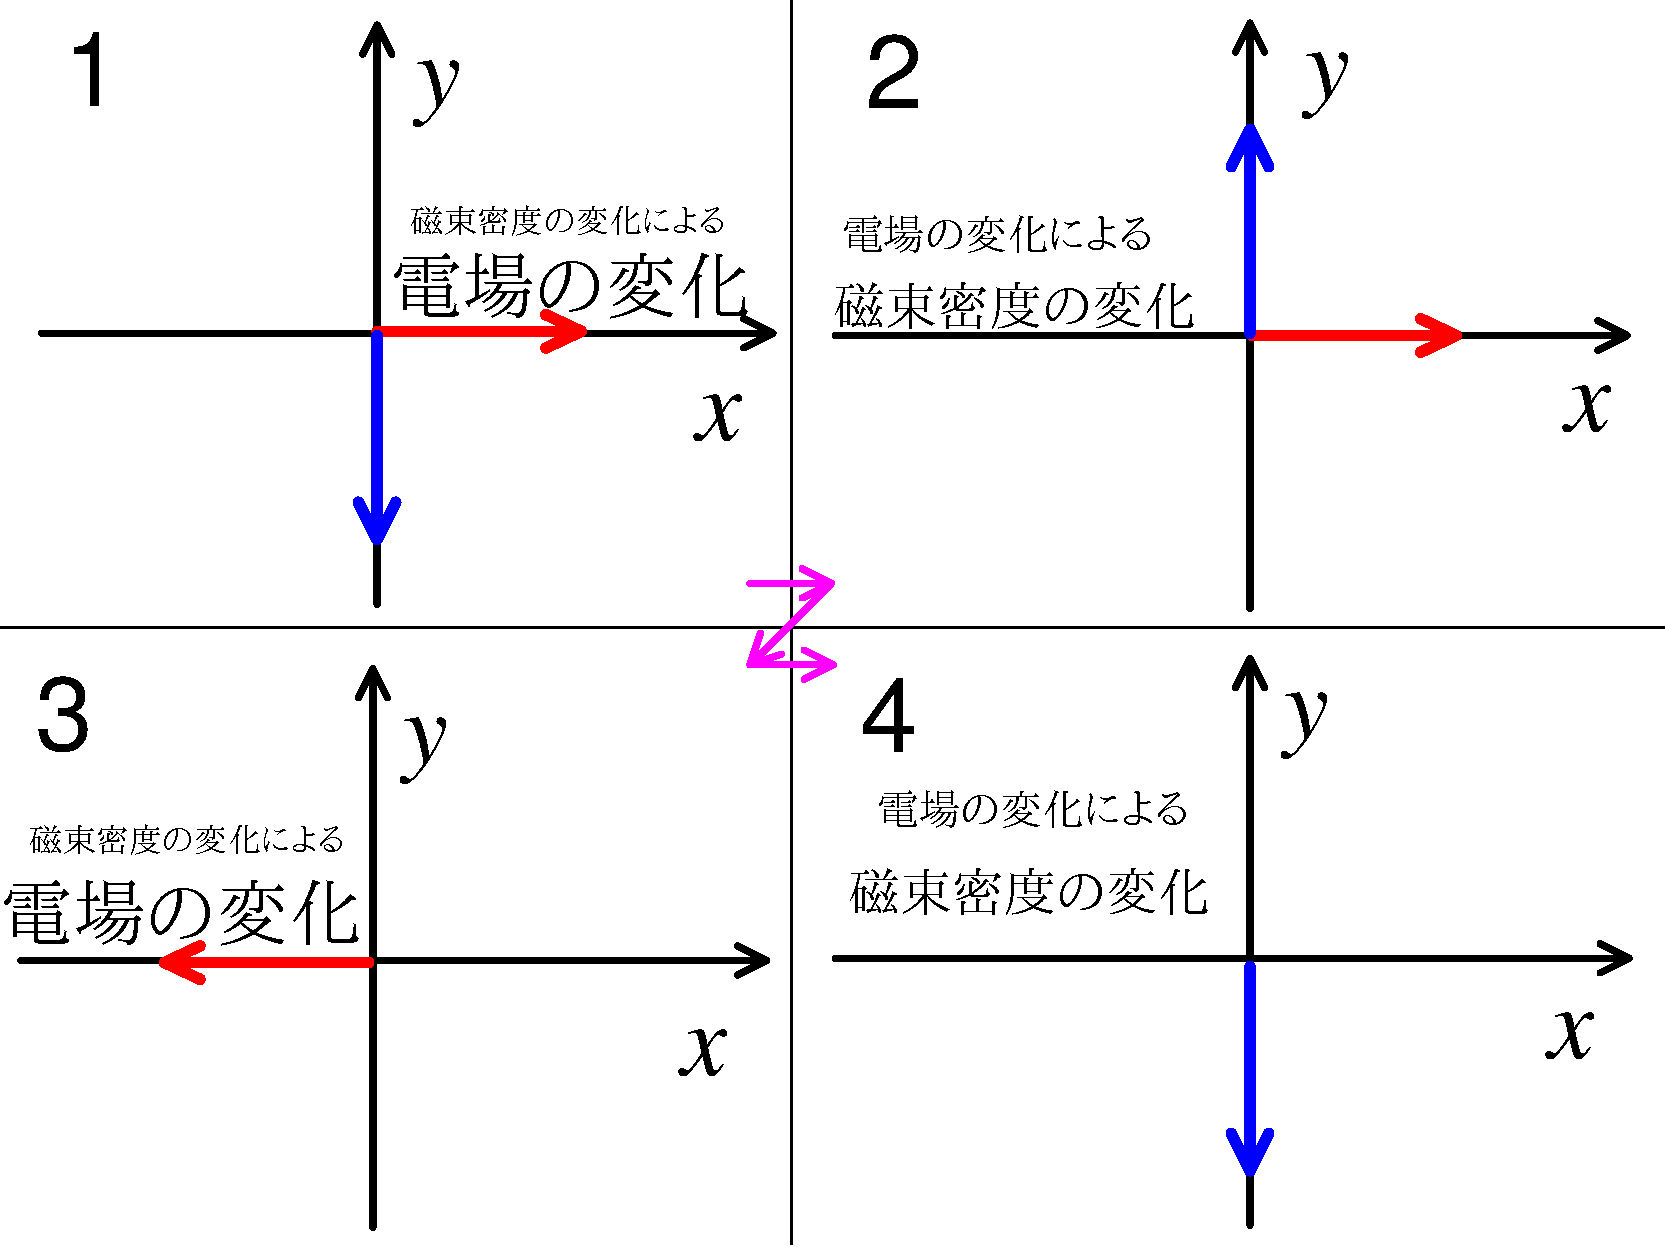
\includegraphics[keepaspectratio, width=6.5cm,height=6cm,clip]{denjiha1.pdf}
                        \caption{原点における電場と磁束密度の変化のイメージ}
                        \label{fig:denjiha1}
                \end{center}
            \end{figure}

            \begin{figure}[hbt]
                \begin{center}
                        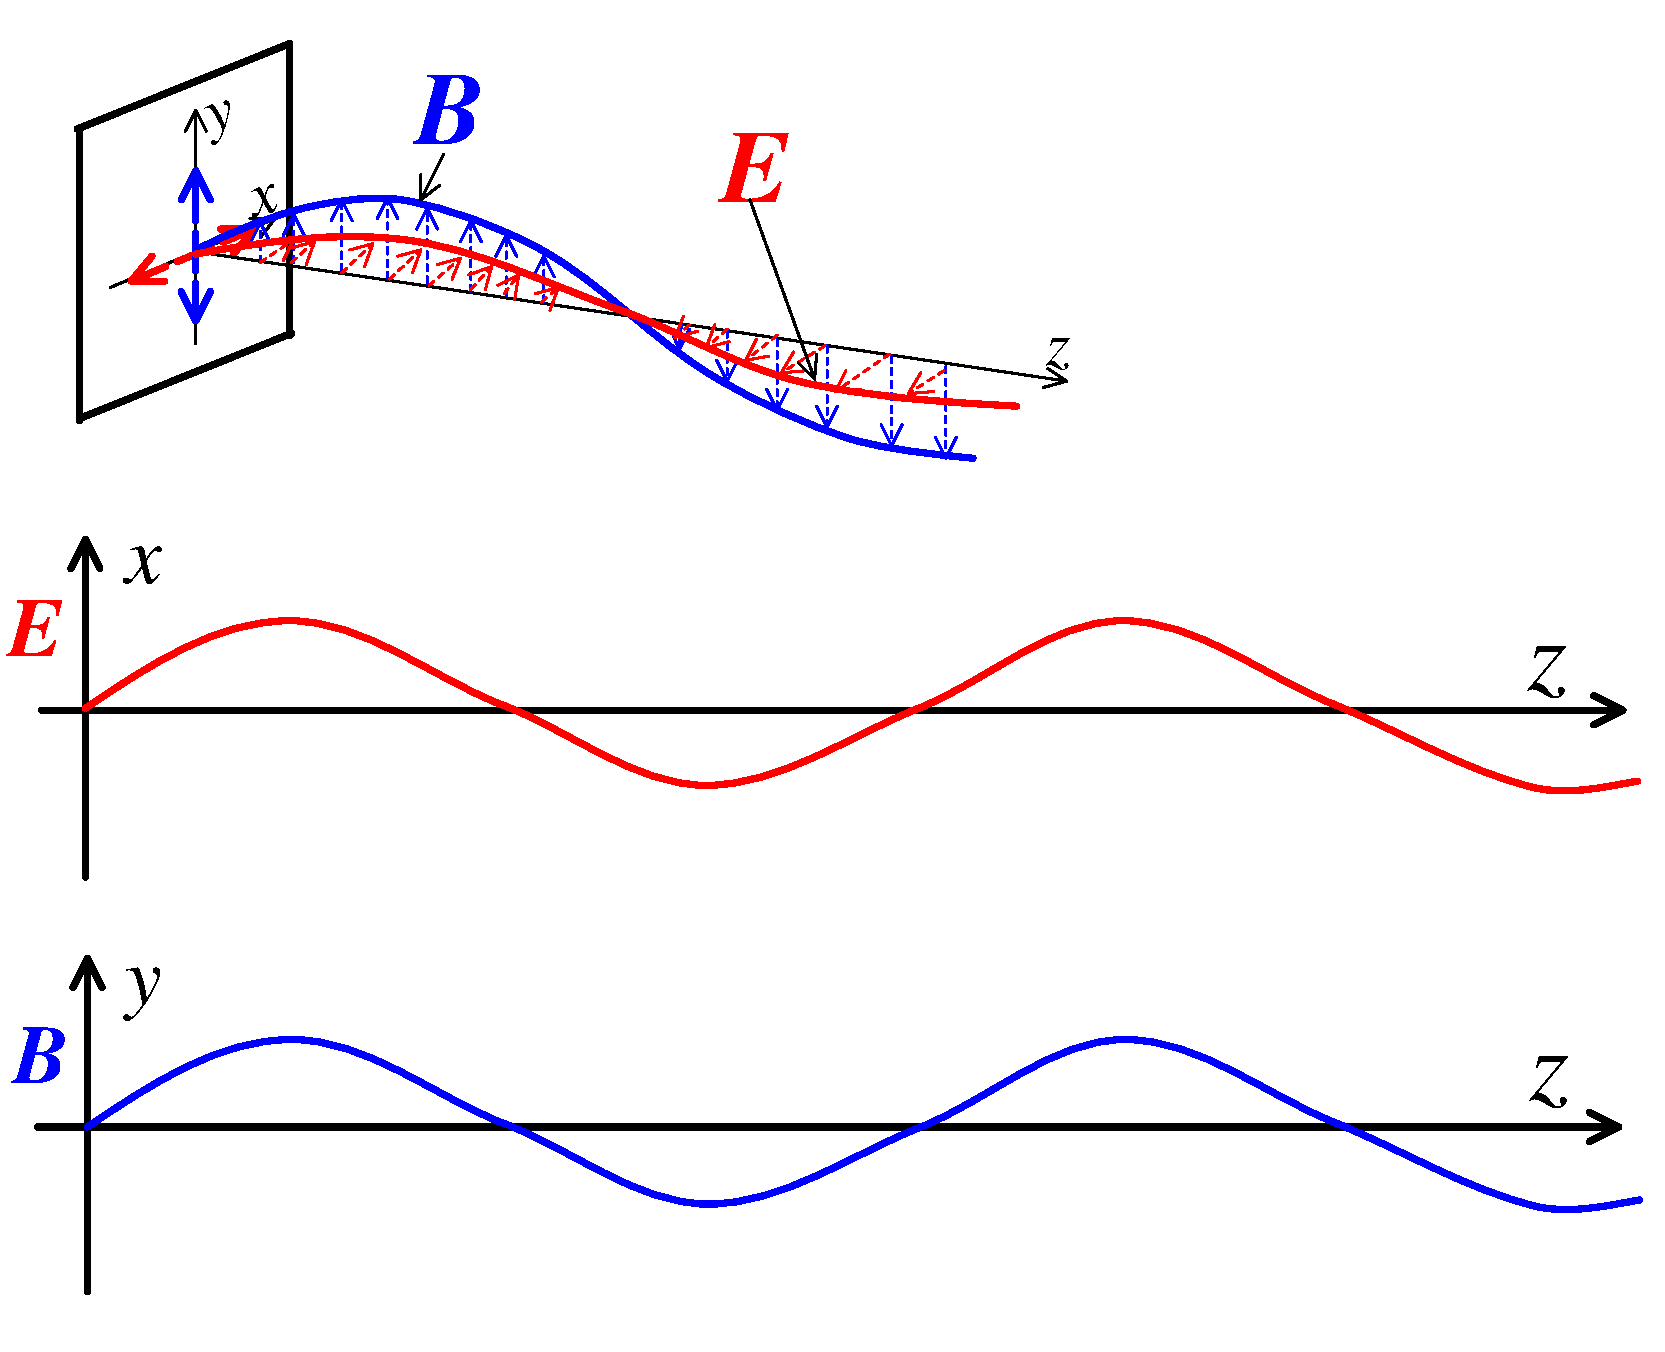
\includegraphics[keepaspectratio, width=6.5cm,height=6cm,clip]{denjiha2.pdf}
                        \caption{電磁波の伝搬のイメージ}
                        \label{fig:denjiha2}
                \end{center}
            \end{figure}

%   %==========================================================================
%   %  SubSection
%   %==========================================================================
    \subsection{電磁場のエネルギー と ポインティング・ベクトル}
        \begin{mycomment}
            電磁波は真空中を伝わる.となると,真空中にも電磁気的なエネルギーが
            蓄えられていると考えられよう.そこで,ここでは真空中に電磁波が存在しているとき,
            この空間に蓄えられている電磁気的なエネルギーについて考える.
        \end{mycomment}

        電磁場におけるエネルギー保存の法則を導く.

        ファラデーの電磁誘導の法則の両辺と,磁束密度 $\bB$ との内積をとり,
                                \begin{align}
                                \bB\cdot\left(\mathrm{rot\,} \bE \right)
                                &= \bB\cdot\left(-\frac{\rd \bB}{\rd t}\right).
                                \end{align}
        右辺を左辺に移項して整理すれば,
                                \begin{align}\label{eq:denyu11}
                                \bB\cdot\left(\frac{\rd \bB}{\rd t}
                                +\mathrm{rot\,} \bE\right)
                                &=0.
                                \end{align}

        次に,アンペール$=$マクスウェルの法則の両辺と,電場 $\bE$ の内積をとり,
                                \begin{align}\label{eq:MAs11}
                                \bE\cdot\mu_{0}\left(\bi+
                                \varepsilon_{0}\frac{\rd \bE}{\rd t}
                                \right)
                                &=\bE\cdot\left(\mathrm{rot\,}
                                \bB\right)
                                \notag \\
                                \Leftrightarrow \quad
                                \bE\cdot\left(
                                \varepsilon_{0}\mu_{0}\frac{\rd \bE}{\rd t}
                                -\mathrm{rot\,}\bB\right)
                                &=-\mu_{0}\bE\cdot\bi
                                \notag \\
                                \Leftrightarrow \quad
                                \bE\cdot\left(
                                \varepsilon_{0}\mu_{0}\frac{\rd \bE}{\rd t}
                                -\mathrm{rot\,}\bB\right)
                                &=-\mu_{0}\bE\cdot\bi
                                \end{align}
        とする.そして,式(\ref{eq:denyu11})と式(\ref{eq:MAs11})の両辺の和をとる.
                                \begin{align}
                                &-\mu_{0}\bE\cdot\bi \notag \\
                                &\quad =
                                \bB\cdot\left(\frac{\rd \bB}{\rd t}
                                +\drot \bE\right)
                                +\bE\cdot\left(
                                \varepsilon_{0}\mu_{0}\frac{\rd \bE}{\rd t}
                                -\drot \bB\right).
                                \end{align}
        右辺と左辺を入れ替えた
                \footnote{
                        A4紙の二段組にした場合,式が一行で納まらなかった.
                }.
            右辺を展開すると,
                                \begin{align}\label{elect_Energy1}
                                &-\mu_{0}\bE\cdot\bi \notag \\
                                &\quad =
                                \bB\cdot\frac{\rd \bB}{\rd t}
                                +\bB\cdot\drot\bE
                                +\bE\cdot\varepsilon_{0}\mu_{0}\frac{\rd \bE}{\rd t}
                                -\bE\cdot\drot\bB.
                                \end{align}

        ところで,任意のベクトル $\bX(t)$ に対して以下の式が成立する.
                                \begin{align}
                                \bX (t)\cdot\frac{\rd \bX (t)}{\rd t}=\frac{1}{2} \frac{\rd \bX(t)^{2}}{ \rd t} .
                                \end{align}
                                \begin{quotation}\small
                                                                なぜなら,
                                \begin{align*}
                                \frac{\rd \bX^{2}}{\rd t}&=\frac{\rd (\bX\cdot \bX)}{\rd t} \\ \notag \\ \notag
                                &=\bX\cdot\frac{\rd  \bX}{\rd t}+\frac{\rd  \bX}{\rd t}\cdot\bX \\ \notag \\ \notag
                                &=2\bX\cdot\frac{\rd \bX}{\rd t}\\ \notag \notag \\
                                \therefore\quad
                                \bX \cdot\frac{\rd \bX }{\rd t}&=\frac{1}{2} \frac{\rd \bX^{2}}{ \rd t} .
                                \end{align*}
                                \end{quotation}

        従って,式(\ref{elect_Energy1})の第1項と第3項を以下のように書き換えることができる.
                                \begin{align*}
                                &-\mu_{0}\bE\cdot\bi \notag \\
                                &\quad = \frac{1}{2} \frac{\rd \bB^{2}}{ \rd t}
                                +\bB\cdot\mathrm{rot\,} \bE
                                +\varepsilon_{0}\mu_{0}\frac{1}{2} \frac{\rd \bE^{2}}{ \rd t}
                                -\bE\cdot\mathrm{rot\,}\bB.
                                \end{align*}
        整理して,
                                \begin{align}
                                &-\mu_{0}\bE\cdot\bi \notag \\
                                &\quad = \frac{1}{2} \frac{\rd }{ \rd t}\left(\bB^{2}
                                +\varepsilon_{0}\mu_{0}\bE^{2}\right)
                                +\bB\cdot\mathrm{rot\,} \bE
                                -\bE\cdot\mathrm{rot\,}\bB.
                                \end{align}
        ここで,左辺の第3項と第4項は,以下のベクトル解析の恒等式を適用してまとめることができる.その公式とは,
        任意の2つのベクトル $\bX$,$\bY$ に対して,
                                \begin{align}
                                \bY\cdot\drot\bX - \bX\cdot\drot\bY =\ddiv(\bX\times\bY).
                                \end{align}
        この恒等式を,上式の左辺第3項と第4項に適用して,式変形すれば,
                                \begin{align}\label{eq:EB_energy}
                                \frac{1}{2} \frac{\rd}{\rd t}\left(\bB^{2}
                                +\varepsilon_{0}\mu_{0}\bE^{2}\right)
                                +\ddiv(\bE\times\bB)
                                =-\mu_{0}\bE\cdot\bi
                                \end{align}
        これを次のように書いてみる.
                                \begin{align}
                                        \ddiv(\bE\times\bB)
                                        + \frac{\rd}{\rd t}
                                          \left\{\frac{1}{2}
                                            \left(
                                              \bB^{2} + \varepsilon_{0}\mu_{0}\bE^{2}
                                            \right)
                                          \right\}
                                        = -\mu_{0}\bE\cdot\bi.
                                \end{align}
        さらに,
                \begin{align}
                        \bS &= \bE\times\bB \,,\,\\
                        W   &= \frac{1}{2} \left(\bB^{2}+\varepsilon_{0}\mu_{0}\bE^{2}\right)
                \end{align}
        と置くと,
            \begin{align}\label{eq:EB_energy}
                \ddiv \bS + \frac{\rd}{\rd t} W = -\mu_{0}\bE\cdot\bi.
            \end{align}
        こうしてみると,式の形が電荷保存の法則の式に似ている.電荷保存の法則は次のように記述された.
            \begin{align}
                 \ddiv\bi + \frac{\rd }{\rd t} \rho = 0.
            \end{align}
        電磁場のエネルギーの式(\ref{eq:EB_energy})の $\bS$ を
        電荷保存の法則の式の電流 $\bi$ と対応させて,
        また,$W$ の部分を電荷密度 $\rho$ と対応させて両式を比較してみよう.

        電荷保存の法則の式の意味は,「電荷の時間変化(つまり電荷の移動)が電流を発生させている」ということであった.
        これを電磁場のエネルギーの式に当てはめて考えると,
        $\left(\bB^{2}+\varepsilon_{0}\mu_{0}\bE^{2}\right)/2$ という
        量の時間変化が,$\ddiv(\bE\times\bB)$ という
        量を生じさせていることになる.また,右辺の電場と電流の積 $-\mu_{0}\bE\cdot\bi$ は
        電荷が電場より受ける単位時間あたりの仕事である.そこで,
        $\left(\bB^{2}+\varepsilon_{0}\mu_{0}\bE^{2}\right)/2$ を \textbf{電磁場のエネルギー密度},
        $\bE\times\bB$ を \textbf{ポインティング・ベクトル} とよぶことにすれば
            \footnote{
                ポインティング・ベクトル:\;Poynting vector であり,ポインティング(Poynting)は
                John Henry Poynting,(1852.9.9-- 1914.3.30,イギリス)
                という人の名前に由来する.
                pointingではない.
            },
        「電磁場のエネルギー密度の変化が,ポインティング・ベクトルを生じさせる」と
        表現される.




%===================================================================================================
%  Chapter : その他の電磁気学的現象
%  説明    : その他の電磁気現象を学習する.
%===================================================================================================
\chapter{その他の電磁気学的現象}
%   %-----------------------------------------------------------------------------------------------
%   %  Input
%   %    File Name : PhysNote_EM_2nd_Phenomenon.tex
%   %    説明      : その他の電磁気現象を学習する.
%   %                ・トムソン効果とか,ゼーベック効果とか,ゼーマン効果とか,いろいろ.
%   %-----------------------------------------------------------------------------------------------
        %===================================================================================================
%  Chapter : その他の電磁気学的現象
%  説明    : その他の電磁気現象を学習する.
%===================================================================================================
    %=======================================================================
    %  Section
    %=======================================================================
    \section{電気双極子}

    %=======================================================================
    %  SubSection
    %=======================================================================
    \section{熱電効果}
        %===================================================================
        %  SubSection
        %===================================================================
        \subsection{はじめに}
            ここでは,熱と電磁気とに関係する現象を考える.\textbf{熱電効果} と
            は,熱によって電流を生じさせる現象のことをいう.例えば,一様な物体
            があったとして,この物体の一部に熱を与えて,周囲よりも高温にしてみ
            る.この時,物体には温度勾配が生じる.熱い部分のエネルギーは冷たい
            う部分よりも高いので,当然,熱した部分の原子の持つ電子も,冷たい部
            分の電子よりも活発に運動していることだろう.活発な電子はその周囲に
            拡散することが容易に想像できる.この電子の拡散こそが,電流であり,
            熱電効果とよばれる理由である.

        %===================================================================
        %  SubSection
        %===================================================================
        \subsection{トムソン効果}\label{subsec:ThomsonEffect}

        %===================================================================
        %  SubSection
        %===================================================================
        \subsection{ペルチェ効果}

        %===================================================================
        %  SubSection
        %===================================================================
        \subsection{ゼーベック効果}

    %=======================================================================
    %  Section
    %=======================================================================
    \section{ゼーマン効果}\label{subsec:ZeemanEffect}
        原子にある程度エネルギーを与えると,その原子内の電子がエネルギー
        を吸収する.そして,電子のエネルギーがある一定値を超えると,エネル
        ギーを抱えきれなくなり,電磁波としてそれを放出する.このとき放出さ
        れる電磁波の波長は原子ごとに決まっている.一般に,放出される電磁波
        の波長は複数である.つまり,原子はエネルギーを外部から与えると,決
        まったいくつかの波長の電磁波を放出する.この原子が出す複数の波長の
        電磁波のことを,\textbf{原子スペクトル} という.また,そのひとつひ
        とつを \textbf{原子スペクトル線} という.

        単一の波長しか放出しない原子
            \footnote{
                スペクトル線をひとつしか持たない原子のこと.
            }
        も存在する.しかし,磁束密度中でエネルギー
        を与えた場合,それが複数種類の電磁波を放出するようになる
            \footnote{
                スペクトル線が2つ以上に分裂するということ.
            }.
        この現象を \textbf{ゼーマン効果} という.

    %=======================================================================
    %  Section
    %=======================================================================
    \section{電子の実験的発見}
        電子は,どのようにしてその存在が認められたのだろうか.
            \begin{figure}[hbt]
                \begin{center}
                    \includegraphicslarge{ThomomExpElec001.pdf}
                    \caption{トムソンの陰極線の実験}
                    \label{fig:ThomomExpElec001}
                \end{center}
            \end{figure}




%===================================================================================================
%  Chapter : 共変形式のマクスウェル方程式
%  説明    : マクスウェル方程式を,ベクトルポテンシャルA とスカラーポテンシャルphi を
%            用いて表す.また,ゲージ変換についても考える.特殊相対性理論への導入も,
%            マクスウェル方程式のガリレイ変換ができないことを通して,行う.
%            その後,電磁ポテンシャルを導入し,マクスウェル方程式を共変形式に書き換える.
%===================================================================================================
\chapter{共変形式のマクスウェル方程式}
%   %-----------------------------------------------------------------------------------------------
%   %  Input
%   %    File Name : PhysNote_EM_2nd_Potential.tex
%   %    説明      : 量子力学や相対性理論に馴染みやすいように,
%   %                マクスウェル方程式をポテンシャル表示に書き換える.
%   %-----------------------------------------------------------------------------------------------
        %===================================================================================================
%  Chapter : マクスウェル方程式のポテンシャル表示
%  説明    : マクスウェル方程式を,ベクトルポテンシャルA とスカラーポテンシャルphi を
%            用いて表す.また,ゲージ変換についても考える.特殊相対性理論への導入も,
%            マクスウェル方程式のガリレイ変換ができないことを通して,行う.
%===================================================================================================
%   %==========================================================================
%   %  Section
%   %==========================================================================
    \section{ポテンシャルの導入}
        \begin{mycomment}
            電磁気学を相対性理論や量子力学で扱うとき,
            電場や磁束密度をそのままの形で表現するよりも,
            ポテンシャルを用いて表現したほうが
            都合がよい.そこでここでは,
            電場と磁束密度をポテンシャル表記することを考える.

            その方法は,まず,磁束密度に対するガウスの法則から,
            ベクトルポテンシャルを定義 $\bA$ し,
            この $\bA$ によって,磁束密度を
            表現することを考える.
            そして,ベクトルポテンシャルによって表現された
            磁束密度を電磁誘導の法則に代入することにより,
            電場のポテンシャル表記する.このとき,電位(電気的なスカラーポテンシャル)と電場の関係
            を考慮する必要がある.
        \end{mycomment}
%       %======================================================================
%       %  SubSection
%       %======================================================================
        \subsection{スカラーポテンシャル:$\phi$}
            スカラーポテンシャルとは,電位 $\phi$ のことである.
            これから,マクスウェル方程式を $\phi$ を用いた表現に書き直すことを
            試みる.

%       %======================================================================
%       %  SubSection
%       %======================================================================
        \subsection{ベクトルポテンシャル:$\bA$}
            ポテンシャルを用いて電場や磁束密度を表現することを考える.
            まず,磁束密度について考える.磁束密度は,
            ガウスの法則により,$\mathrm{div\,}\bB=0$ を満たしている.
            このことに注目しながら,次のベクトル解析の恒等式を考える.
            あるベクトル $\bA$ に対して,
            \begin{align}\label{div_rot}
            \mathrm{div\,rot\,}\bA=0
            \end{align}
            回転の発散は常に 0 であるということを意味している.式(\ref{div_rot})の
            ベクトル $\mathrm{rot\,}\bA$ を
            磁束密度 $\bB$ に置き換えれば,
            すなわち,
            \begin{align}\label{rotA}
            \bB=\mathrm{rot\,}\bA
            \end{align}
            とすれば,
            以下の恒等式を
            得られる.
            \begin{align}\label{div_rotA}
            \mathrm{div\,}\bB=0
            \end{align}
            式(\ref{rotA})のように磁束密度を表すことによって,
            ガウスの法則が数学的に自動的に成り立つのである.
            この式(\ref{rotA})を満たすようなベクトル $\bA$ の
            ことを \textbf{ベクトルポテンシャル} という.

            物理的には,ベクトルポテンシャルという概念を
            理解することは難しいが,ポテンシャルを
            基礎に置いた理論は現代では主流である.
            解析力学,量子力学や相対性理論との関連を考えるとき,
            ベクトルポテンシャルの概念は便利な道具として用いられる.
            ベクトルポテンシャルの実在性は,\textbf{Aharonov=Bohm効果} という
            現象によって確認されている.この効果については,量子力学の
            知識が必要である.

%       %======================================================================
%       %  SubSection
%       %======================================================================
        \subsection{ベクトルポテンシャル $\bA$ の形}
            前項目では,ベクトルポテンシャル $\bA$ を磁束密度がガウスの法則を満たすように定義したが,
            具体的な形はまだわかっていない.$\bA$ は電流 $\bi$ と 位置 $\br$ で表せる.
            以下で計算し,確認してみよう.

            ベクトルポテンシャル $\bA$ の定義は磁束密度 $\bB$ に対するガウスの法則から
            定義された.
                \begin{equation*}
                    \bB := \drot \bA
                \end{equation*}
            ところで,磁束密度はビオ$=$サバールの法則によって記述される.
            そこで,ビオ$=$サバールの法則を式変形していき,
            上の磁束密度とベクトルポテンシャルの関係式の形へ誘導し,
            ベクトルポテンシャルに対応する部分を見ることで,ベクトルポテンシャルの形を考えていく.

            最初に,式変形につかう公式を2つ確認する.
            一つは $\br'$ に関する $\dgrad$ として,
                \begin{align}\label{eq:grad_r}
                    \dgrad_{\br'} \left( \frac{1}{| \br -\br' |}\right)
                    =-\frac{\br-\br'}{| \br-\br' |^{3}}.
                \end{align}
            もう一つは,sを任意のスカラー
                \footnote{
                    スカラーとは,大きさのみを数である.
                    ベクトルが複数の数の組みで表現されるのに対し,
                    スカラーは1つの数で表現される.
                }
            ,$\bU$ を任意のベクトルとして,
                \begin{align}\label{eq:grad_sU0}
                    \drot(s\bU\,) = s\,\drot\bU - \bU\times(\dgrad s)
                \end{align}
            というベクトル解析の公式である.今回はこの公式の $\bU$ は
            定電流 $\bi(\br)$ に対応させるので,定数ベクトルとして
            の扱いになる.$\bU$ を定数ベクトルと見たとき,この公式(\ref{eq:grad_sU0})は
            次のように計算される.
                \begin{align}\label{eq:grad_sU}
                    \drot(s\bU\,) = - \bU\times(\dgrad s).
                \end{align}
            今回の式変形では公式を変形した式(\ref{eq:grad_sU})を
            用いる.

            それでは,式変形に執りかかろう.
            ビオ$=$サバールの法則は以下のようであった.
                \begin{align*}
                    \bB(\br)
                    &=\frac{\mu_{0}}{4\pi}
                    \int\frac{\bi(\br')\times
                    (\br-\br')
                    }{|\br-\br'|^{3}}\df V' \\
                    &=\frac{\mu_{0}}{4\pi}
                    \int\bi(\br')\times
                    \frac{\br-\br'}
                    {|\br-\br'|^{3}}\df V'
                \end{align*}
            一番右の式に先ほどの公式(\ref{eq:grad_r})を用いると,
                \begin{align}
                    \bB(\br)
                    =-\frac{\mu_{0}}{4\pi}
                    \int\bi(\br')\times
                    \dgrad_{\br'} \left( \frac{1}{| \br -\br'|}\right)
                    \df V'
                \end{align}
            右辺に,先ほど記述したベクトル解析の公式 $\drot(s\bU\,) = - \bU\times(\dgrad s)$ を
            使うと,
                \begin{align}\label{eq:vector_Pt_A}
                    \bB(\br)
                    &=\int \drot \frac{\mu_{0}}{4\pi}\frac{\bi(\br\,')}{| \br -\br'|}\df V' \notag \\
                    &=\drot \int \frac{\mu_{0}}{4\pi}\frac{\bi(\br\,')}{| \br -\br'|}\df V'
                \end{align}
            となる.この式(\ref{eq:vector_Pt_A})と,ベクトルポテンシャルと磁束密度の関係式 $\bB=\drot\bA$ の
            ベクトルポテンシャル $\bA$ に対応する部分に注目すれば,
                \begin{align}
                    \bA(\br)
                    =\int\frac{\mu_{0}}{4\pi}\frac{\bi(\br\,')}{| \br -\br'|}\df V'
                \end{align}
            を得る.以上で,ベクトルポテンシャルの具体的な形を得ることができた.

%       %======================================================================
%       %  SubSection
%       %======================================================================
        \subsection{磁束密度のポテンシャル表示}
            今までの議論で,散々書かれてきたが,改めて記載しておこう.
            磁束密度 $\bB$ は,ベクトルポテンシャル $\bA$ を用いると,以下のように
            表現できる.
                \begin{align}
                    \bB = \drot \bA.
                \end{align}

%       %======================================================================
%       %  SubSection
%       %======================================================================
        \subsection{電場のポテンシャル表示}
            前項目では,磁束密度をベクトルポテンシャルを用いて
            表現することを考えた.それは,$\bB=\mathrm{rot\,}\bA$ の
            様に表現される.さて,ここでは電場をポテンシャルで表現することを考える.
            そのためは,$\bB=\mathrm{rot\,}\bA$ を用いる.
            どう用いるかといえば,この式をファラデーの電磁誘導の法則に代入するのである.
            ファラデーの電磁誘導の法則は
            \begin{align}
            \drot \bE &= -\frac{\rd \bB}{\rd t}
            \end{align}
            であった.この式に $\bB=\mathrm{rot\,}\bA$ を
            代入すると,
            \begin{align}
            \mathrm{rot\,} \bE &= -\frac{\rd(\mathrm{rot\,}\bA)}{\rd t}\notag \\ \notag \\
            \Leftrightarrow
            \mathrm{rot\,}\frac{\rd\bA}{\rd t}
            +\mathrm{rot\,} \bE&=0 \notag \\
            \Leftrightarrow
            \mathrm{rot\,}\left(\frac{\rd\bA}{\rd t}
            + \bE\right) &=0
            \end{align}
            となる.一般的に,この式の解は
            \begin{align}
            \frac{\rd\bA}{\rd t}
            + \bE&=-\mathrm{grad\,}\phi
            \end{align}
            と書かれる.但し数学的には,右辺の負符号は必要ない.負の符号を付けたのは,
            電位の定義によるものである.
            従って,電場をポテンシャル表示すると,
            \begin{align}
            \bE&=-\frac{\rd\bA}{\rd t}-\mathrm{grad\,}\phi
            \end{align}
            となる.


%   %==========================================================================
%   %  Section
%   %==========================================================================
    \section{マクスウェル方程式のポテンシャル表示}
    \begin{mycomment}
            さて,以上の計算から,電場と磁束密度の
            ポテンシャル表示を確認した.具体的には,
            電場と磁束密度はそれぞれ,
            スカラーポテンシャル $\phi$ とベクトルポテンシャル $\bA$ を
            用いて,
            \begin{align}\label{pt_EB}
            \begin{cases}
            \displaystyle\bE=-\frac{\rd\bA}{\rd t}-\dgrad\phi \\  \notag \\
            \vspace{2mm}
            \displaystyle\bB=\drot\bA
            \end{cases}
            \end{align}
            のように表現されることが分かった.
            このポテンシャル表示が示すように,電場や磁束密度はポテンシャルから導かれると
            考えることも可能である.

            このポテンシャル表示を導く課程で,ファラデーの電磁誘導の法則と
            磁束密度に対するガウスの法則を用いた.そして,マクスウェル方程式の残りの
            もう二つの法則,すなわち,アンペール$=$マクスウェルの法則と電場に対するガウスの法則
            のそれぞれに,上で確認した電場と磁束密度を代入すれば,
            それによって得た方程式と式(\ref{pt_EB})はマクスウェル方程式と
            同等であると考えられる.では,実際に計算していくことにする.
    \end{mycomment}


%       %======================================================================
%       %  SubSection
%       %======================================================================
        \subsection{アンペール$=$マクスウェルの法則の変形}
            アンペール$=$マクスウェルの法則は以下のように書かれることは前に確認した.
            すなわち,
            \begin{align}
            \left(\bi+
            \varepsilon_{0}\frac{\rd \bE}{\rd t}
            \right)
            =\frac{1}{\mu_{0}}\drot\bB
            \end{align}
            である.この方程式に,電場や磁束密度のポテンシャル表示式(\ref{pt_EB})を
            考慮すると,以下のようになる.
            \begin{align}\label{AM_phi_A}
            \bi+
            \varepsilon_{0}\frac{\rd }{\rd t}
            \left( -\frac{\rd\bA}{\rd t}-\dgrad\phi\right)
            =\frac{1}{\mu_{0}}\drot\left(\drot\bA\right)
            \end{align}

            さてここで,ベクトル解析による恒等式を用いる.それは,任意のベクトルを $\bC$ としたとき,
            \begin{align}\label{rotrot_C_gdCdgC}
            \drot\drot\bC:=
           \dgrad\ddiv\bC - \Delta \bC
            \end{align}
            が成り立つというものである.この恒等式(\ref{rotrot_C_gdCdgC})を
            用いれば,式(\ref{AM_phi_A})は
            \begin{align}
            &\frac{1}{\mu_{0}}\left(\dgrad\ddiv\bA - \Delta \bA\right) \notag \\
            &\quad=\bi+ \varepsilon_{0}\frac{\rd }{\rd t} \left( -\frac{\rd\bA}{\rd t}-\dgrad\phi\right) \notag \\
            &\Leftrightarrow -\mu_{0}\bi \notag \\
            &\quad=\left(\Delta -\frac{1}{c^{2}}\frac{\rd^{2}}{\rd t^{2}}\right)\bA
             -\mathrm{grad\,}\left( \ddiv\bA + \frac{1}{c^{2}}\frac{\rd \phi}{\rd t}\right)
            \end{align}
            と変形される.ここで,$c=1/\sqrt{\varepsilon_{0}\mu_{0}}$ とおいた.
            $c$ は波動の位相速度で,特にこの場合は光速の意味を持つ.
            注意しておくことは,
            この式はもはやアンペール$=$マクスウェルの法則を
            示すものではないということである.

%       %======================================================================
%       %  SubSection
%       %======================================================================
        \subsection{電場に対するガウスの法則の変形}
            電場に対するガウスの法則を書き下すと,
            \begin{align}
            \ddiv\bE
            =\frac{1}{\varepsilon_{0}}\rho
            \end{align}
            である.この式に,ポテンシャル表示された
            電場 $\displaystyle\bE = -(\rd\bA/\rd t) -\mathrm{grad\,}\phi$ を
            代入すると,
            \begin{align}
            \ddiv\left(-\frac{\rd\bA}{\rd t}-\mathrm{grad\,}\phi\right)
            =\frac{1}{\varepsilon_{0}}\rho \notag \\  \notag \\
            \Leftrightarrow
            -\frac{\rd(\mathrm{div\,}\bA)}{\rd t}-\mathrm{div\,grad\,}\phi
            =\frac{1}{\varepsilon_{0}}\rho
            \end{align}
            そして,$\Delta:=\mathrm{div\,grad\,}$ ということに注意すれば,
            \begin{align}
            \frac{\rd(\mathrm{div\,}\bA)}{\rd t}+\Delta\phi
            =-\frac{1}{\varepsilon_{0}}\rho
            \end{align}
            となる.ここで,少々トリッキーな操作を行う.
            この式の両辺に $-\varepsilon_{0}\mu_{0}(\rd^{2} \phi/\rd t^{2})$ を加える.
            \begin{align}
            &\frac{\rd(\mathrm{div\,}\bA)}{\rd t}+\Delta\phi
            -\varepsilon_{0}\mu_{0}\frac{\rd^{2} \phi}{\rd t^{2}}
            =-\frac{1}{\varepsilon_{0}}\rho -\varepsilon_{0}\mu_{0}\frac{\rd^{2} \phi}{\rd t^{2}}\notag \\ \notag \\
            &\Leftrightarrow\,
            \left(\Delta
            -\frac{1}{c^{2}}\frac{\rd^{2} }{\rd t^{2}}\right)\phi
            +\frac{\rd}{\rd t}\left(\mathrm{div\,}\bA
            +\frac{1}{c^{2}}\frac{\rd \phi}{\rd t}
            \right)
            =-\frac{1}{\varepsilon_{0}}\rho
            \end{align}

            これで,とりあえずの式変形が終了した.この後に,
            これら4つの式を,次に確認する \textbf{Lorentz ゲージ} という
            ゲージを導入し,もう少し表現を簡略化する.その前に,とりあえず
            今までに得られたマクスウェル方程式と等価な方程式をまとめておく.
                    \begin{myshadebox}{マクスウェル方程式のポテンシャル表示}
                        以下の方程式群は,マクスウェル方程式を,ベクトルポテンシャルと
                        スカラーポテンシャルを用いた表現に書きなおしたものであり,
                        先に導出したマクスウェル方程式と(数学的に)同等の内容である.
                        \begin{align}
                            \bE&=-\displaystyle
                            \frac{\rd\bA}{\rd t}-\mathrm{grad\,}\phi \\ \notag \\
                            \vspace{2mm}
                            \bB&=\mathrm{rot\,}\bA
                        \end{align}
                        \begin{align}
                            &-\mu_{0}\bi  \\\,\vspace{2mm}  \notag \\
                            &=\left(\Delta
                            -\frac{1}{c^{2}}\frac{\rd^{2}}{\rd t^{2}}\right)\bA
                            -\mathrm{grad\,}\left( \mathrm{div\,}\bA
                            +\frac{1}{c^{2}}\frac{\rd{\phi}}{\rd t}\right) \\
                            &-\frac{1}{\varepsilon_{0}}\rho \notag \\
                            &=\left(\Delta
                            -\frac{1}{c^{2}}\frac{\rd^{2} }{\rd t^{2}}\right)\phi
                            +\frac{\rd}{\rd t}\left(\mathrm{div\,}\bA
                            +\frac{1}{c^{2}}\frac{\rd \phi}{\rd t}
                            \right)
                        \end{align}
                    \end{myshadebox}

                このままでは式の形がややこしいので,
                次に \textbf{ゲージ変換} を確認して,
                \textbf{ローレンツ条件} を導入しよう.


%       %======================================================================
%       %  SubSection
%       %======================================================================
        \subsection{ゲージ変換}
            電場 $\bE$ と磁束密度 $\bB$ のポテンシャル表示の式は以下のように表現されることは,
            前項目で既に確認している.
                    \begin{align}
                            \bE&=-\displaystyle
                            \frac{\rd\bA}{\rd t}-\mathrm{grad\,}\phi \\  \notag \\
                            \vspace{2mm}
                            \bB&=\mathrm{rot\,}\bA
                    \end{align}
            ここで,2つのポテンシャル $\bA$ と $\phi$ を以下のように変換してみる.\\
                        \begin{myshadebox}{ゲージ変換}
                            2つのポテンシャル $\bA$ と $\phi$ の \textbf{ゲージ変換} とは,
                            以下の変換のことをいう.
                            \begin{align}\label{guage1}
                                \bA'&=\bA-\dgrad\chi \\ \notag \\
                                \phi ' &=\phi +\frac{\rd \chi}{\rd t}
                            \end{align}
                        \end{myshadebox}

            ここで,$\chi$ は任意の関数である.
            このように,ポテンシャルを式(\ref{guage1})で変換することを,\textbf{ゲージ変換} という.
            なぜこんな可笑しな変換を考えるかといえば,それは次のような理由による.
            \textbf{ポテンシャルをゲージ変換しても,
            電場と磁束密度は形を変えない}.このことを確認をしておこう.

            まず,電場について考えよう.ゲージ変換をしたポテンシャルでの電場 $\bE\,'$ は,
                    \begin{align}
                            &\bE\,' \notag \\
                            &=-\displaystyle \frac{\rd\bA'}{\rd t}-\mathrm{grad\,}\phi ' \notag \\
                            &=-\frac{\rd}{\rd t}\left( \bA-\dgrad\chi \right)
                            -\dgrad\left( \phi+\frac{\rd \chi}{\rd t} \right) \notag \\
                            &=-\frac{\rd  \bA}{\rd t}+\frac{\rd  (\dgrad\chi)}{\rd t}
                            -\dgrad\phi-\dgrad\left( \frac{\rd \chi}{\rd t} \right) \notag \\
                            &=-\frac{\rd  \bA}{\rd t}+-\dgrad\left( \frac{\rd \chi}{\rd t} \right)
                            -\dgrad\phi-\dgrad\left( \frac{\rd \chi}{\rd t} \right) \notag \\
                            &=-\frac{\rd  \bA}{\rd t}-\dgrad\phi \notag \\
                            &=\bE\notag \\ \notag \\
                            &\therefore\,\,\bE\,'=\bE
                    \end{align}
            よって,ゲージ変換を適用しても,電場の形の変化はない.

            次に,磁束密度について確認しよう.ゲージ変換された磁束密度を $\bB\,'$ とすると,
                    \begin{align}
                    \bB\,'&=\drot\bA' \notag \\
                    &=\drot\left(\bA-\mathrm{grad \chi} \right)\notag \\
                    &=\drot\bA-\mathrm{rot\,grad} \,\chi\notag \\
                    &=\drot\bA\notag \\
                    &=\bB\notag \\
                    \therefore\,\quad\,
                    \bB\,'&=\bB
                    \end{align}
            よって電場と同様に,磁束密度についてもゲージ変換を適用しても,磁束密度の形を変えることはないことが示された.

            以上のように,電場と磁束密度はゲージ変換に対してその形を変化させることは
            ないことを示したが,このことを,電場と磁束密度は \textbf{ゲージ変換に対して不変である} と表現する.

%       %======================================================================
%       %  SubSection
%       %======================================================================
        \subsection{ローレンツ条件}
            ベクトルポテンシャルとスカラーポテンシャルが以下の式ローレンツ条件を満たすと仮定する.
                        \begin{myshadebox}{ローレンツ条件式}
                            \begin{align}
                                \mathrm{div\,}\bA + \frac{1}{c^{2}}\frac{\rd \phi}{\rd t}
                                =0
                            \end{align}
                        \end{myshadebox}

            こうすると,マクスウェル方程式がきれいに整理される.しかし,
            上のローレンツ条件はどうなるか.実は,これは大した問題ではなく,理論にも矛盾を
            引き起こしたりしない.そのことを確認するため,計算してみよう.

            ローレンツ変換式に,ゲージ変換した
            ポテンシャル $\bA'=\bA-\dgrad\chi$,
            $\phi ' =\phi +\left(\rd \chi/\rd t\right)$ を代入して,
                            \begin{align*}
                                &\mathrm{div\,}\bA' + \frac{1}{c^{2}}\frac{\rd \phi '}{\rd t} \notag \\
                                &\quad=\mathrm{div\,}(\bA-\dgrad\chi)
                                +\frac{1}{c^{2}}\frac{\rd}{\rd t}
                                \left(\phi +\frac{\rd \chi}{\rd t}\right) \\ \notag \\
                                &\quad=\mathrm{div\,}\bA
                                -\mathrm{div\,grad\,}\chi
                                +\frac{1}{c^{2}}\frac{\rd \phi}{\rd t}
                                +\frac{1}{c^{2}}\frac{\rd^{2} \chi}{\rd t^{2}} \\ \notag \\
                                &\quad=\mathrm{div\,}\bA
                                +\frac{1}{c^{2}}\frac{\rd \phi}{\rd t}
                                \left(
                                    -\mathrm{div\,grad\,}\chi
                                +\frac{1}{c^{2}}\frac{\rd^{2} \chi}{\rd t^{2}}
                                \right)
                            \end{align*}
            ここで,$\Delta:=\mathrm{div\,grad\,}$ であることに注意して,
                            \begin{align*}
                                &\mathrm{div\,}\bA'
                                +\frac{1}{c^{2}}\frac{\rd \phi '}{\rd t} \\
                                &\quad=
                                \mathrm{div\,}\bA
                                +\frac{1}{c^{2}}\frac{\rd \phi}{\rd t}
                                -\left(
                                    \Delta\chi
                                -\frac{1}{c^{2}}\frac{\rd^{2} \chi}{\rd t^{2}}
                                \right)
                            \end{align*}
            この式で右辺第1項と第2項の和は,ローレンツ条件で 0になるから,
                            \begin{align*}
                                \mathrm{div\,}\bA'
                                +\frac{1}{c^{2}}\frac{\rd \phi '}{\rd t}
                                &=
                                -\left(
                                    \Delta\chi
                                -\frac{1}{c^{2}}\frac{\rd^{2} \chi}{\rd t^{2}}
                                \right)
                            \end{align*}
            と計算される.ゲージ変換しても,ローレンツ変換式を維もできるためには,この式の右辺が0に等しければよく,
            つまり
                            \begin{align}
                                \left(
                                    \Delta\chi
                                -\frac{1}{c^{2}}\frac{\rd^{2} \chi}{\rd t^{2}}
                                \right)
                                =0
                            \end{align}
            が満たされていればよい.この条件を満たすような解 $\chi$ は1つ以上,すなわち,
            複数存在する.しかし,この条件を満たすような解ならば,
            $\chi$ はどのようなものであってもよい.とにかく,そのような解が存在するということを
            確認できればそれでよいのである.
            解である $\chi$ 具体的な形はあまり本質的ではないのだ.以上で確認終了.
            これで安心してローレンツ条件を用いることができる.


            この条件式を用いて,ポテンシャル表記されたマクスウェル方程式
            を整理するとつぎのようになる.
               \begin{myshadebox}{マクスウェル方程式のポテンシャル表示}
                        \begin{align}
                            \bE&=-\displaystyle
                            \frac{\rd\bA}{\rd t}-\mathrm{grad\,}\phi \\ \notag \\
                            \vspace{2mm}
                            \bB&=\mathrm{rot\,}\bA
                    \end{align}
                    \begin{align}
                            \left(\Delta
                            -\frac{1}{c^{2}}\frac{\rd^{2}}{\rd t^{2}}\right)\bA
                            &=-\mu_{0}\bi  \\\,\vspace{2mm} \notag \\
                            \left(\Delta
                            -\frac{1}{c^{2}}\frac{\rd^{2} }{\rd t^{2}}\right)\phi
                            &=-\frac{1}{\varepsilon_{0}}\rho
                    \end{align}
                        \textbf{ローレンツ条件式}
                            \begin{align}
                                \mathrm{div\,}\bA
                                +\frac{1}{c^{2}}\frac{\rd \phi}{\rd t}
                                =0
                            \end{align}
               \end{myshadebox}


                    条件式が1つ多くなるが,マクスウェル方程式はかなり整理された形になったと
                    感じられることと思う(感覚は人それぞれではあるが...)
                      \footnote{
                        くどいようだが,確認しておきたいことがある.式を1つ追加してまでも
                        マクスウェル方程式をポテンシャル表記するのは,後に考える量子力学や相対性理論との
                        かかわりをより深く理解するためである.この理由を改めておくのは,学習意欲を
                        失うことのないようにするためである.
                      }.


%       %======================================================================
%       %  SubSection
%       %======================================================================
        \subsection{ポテンシャル表記の利点}
                    マクスウェル方程式を,電位 $\phi$ とベクトルポテンシャル $\bA$ で
                    表すことで,マクスウェル方程式が数学的に美しい形で表現された.
                    つまり,方程式が解きやすくなったのだ.マクスウェル方程式を解くとは,
                    電場 $\bE$ と磁束密度 $\bB$ を求めることである.元の式で
                    は,$\bE$ と $\bB$ がひとつの方程式に混在している.
                    それに対して,ポテンシャル表記された方程式は,$\phi$ と $\bA$ が
                    分離されている.つまり,元の式から $\bE$,$\bB$ を解くより,
                    ポテンシャル表記された方程式から $\phi$,$\bA$ を求める
                    方が簡単なのである.$\phi$ と $\bA$ さえ求まれば,$\bE$ と $\bB$ は
                    すぐに求められる.数学的解析を行いたい場合には,この
                    ポテンシャル表記された方程式は,とても役に立つ.

                    さらに言えば,ポテンシャル表記された方程式は
                    量子力学や相対性理論との相性がいい.量子力学・
                    相対性理論を学ぶ際には,ポテンシャル表記の方程式を
                    理解していなければならない.

                    もちろん,数式と物理現象との対応を,鮮やかに表現しているのは
                    元の $\bE$ と $\bB$ で表される方程式である.
                    要するに,目的応じて数式的表現を選べるのである.
                    実際の物理現象のイメージを大切にしたい場合は $\bE$ と $\bB$ で
                    表される方程式を使えばいい.
                    問題を解析的(数学的)に解きたい場合はポテンシャル表記の方程式を
                    選べばよい.一度数式で表現された物理現象は,もはや物理現象の
                    数式表現と言うことにとどまらず,純粋に数学的な方程式の問題としても
                    見れるのである.ポテンシャル表記された方程式は,意味がわからないとして
                    避けてしまってはならない.むしろ,これから先の学習で,ポテンシャル
                    表記の方程式はなくてはならないものになるはずである.



%   %-----------------------------------------------------------------------------------------------
%   %  Input
%   %    File Name : PhysNote_EM_2nd_ToSpecialRelativity.tex
%   %    説明      : マクスウェル方程式の共変形式表示への導入
%   %-----------------------------------------------------------------------------------------------
        %===================================================================================================
%  Chapter : マクスウェル方程式のポテンシャル表示
%  説明    : マクスウェル方程式を,ベクトルポテンシャルA とスカラーポテンシャルphi を
%            用いて表す.また,ゲージ変換についても考える.特殊相対性理論への導入も,
%            マクスウェル方程式のガリレイ変換ができないことを通して,行う.
%===================================================================================================
%   %==========================================================================
%   %  Section
%   %==========================================================================
    \section{マクスウェル方程式のガリレイ変換}
        \subsection{マクスウェル方程式に対してガリレイ変換は適用できない}
            マクスウェル方程式をガリレイ変換すると,式の形が変わってしまう.
            つまり,残念ながら,マクスウェル方程式はガリレイ変換に対して不変でない.

            式で示すと,S座標系と S'座標系で式の形が違うということであり,
                \[
                {\nabla}^{2} -\frac{1}{{c}^{2}}\frac{{\rd}^{2}}{{\rd t}^{2}}
                \neq
                {\nabla '}^{2} -\frac{1}{{c}^{2}}\frac{{\rd}^{2}}{{\rd t'}^{2}}
                \]
            ということ.要するに,波動方程式はガリレイ変換にできないので,
            波動方程式をその内部に含むマクスウェル方程式もガリレイ変換に従わないということだ.

            しかし,マクスウェル方程式が間違っているのではない.
            マクスウェル方程式は電磁波など現象を予言できるし,
            電磁気現象を十分に説明できる方程式であり,誤っているとは考えにくい.

            では,何がおかしいのか.実は,そもそも,ガリレイ変換がおかしいのである.
            特殊相対性理論により,ガリレイ変換は,光速よりも十分に遅く等速運動する物体に
            対して有効な変換であることが分かった.より一般的な変換法則はローレンツ変換
            であり,ガリレイ変換はローレンツ変換の特殊な場合
                \footnote{
                    ここでいう特殊な場合とは,光速に対して,とても遅く運動するという状況である.
                }
            に過ぎない.そして,マクスウェル方程式はローレンツ変換に対しては不変である.

            以下で,このことを数式を使いながら考えていこうと思う.
            よく教科書では,
                1) ガリレイ変換を偏微分の公式に形を変えて,
            その後に,
                 2) 電磁波の波動方程式がその偏微分で表されたガリレイ変換の式に不変でないことを示している.
            このノートでも同じような手法をとる.計算課程も詳しく記載しておこう
                \footnote{
                    多くの教科書では,計算が当たり前すぎるためなのか,紙面の都合上の問題なのか,
                    計算過程が示されておらず,結果のみが記されている.
                }.

        \subsection{ガリレイ変換と偏微分演算子}
            \subsubsection{時間微分の計算}
                座標変換により,$S=S'(x',\,t')$ と変換できるとする.
                このとき,合成関数の微分を用いると,\textbf{時間微分} は以下の通り.
                    \begin{align*}
                        \frac{\rd S }{\rd t'} &=   \frac{\rd S }{\rd x } \frac{\rd x }{\rd t'}
                                                + \frac{\rd S }{\rd t } \frac{\rd t }{\rd t'} \\
                                            &=   \frac{\rd x }{\rd t'} \frac{\rd S }{\rd x }
                                                + \frac{\rd t }{\rd t'} \frac{\rd S }{\rd t } \\
                                            &=   \left(
                                                \frac{\rd x }{\rd t'} \frac{\rd   }{\rd x }
                                                + \frac{\rd t }{\rd t'} \frac{\rd   }{\rd t }
                                                \right) S.
                    \end{align*}

                ガリレイ変換の場合,空間座標は $x=x'+Vt'$($V$ は S系と S'系の相対速度)なので,
                    \begin{align*}
                        \frac{\rd x }{\rd t'} = \frac{\rd }{\rd t'} \left( x'+Vt' \right)
                                              = V.
                    \end{align*}
                さらに,
                    \begin{align*}
                        \frac{\rd x}{\rd x'}  = \frac{\rd }{\rd x'} \left( x'+Vt' \right)
                                              = 1
                    \end{align*}
                が成立する.従って,
                    \begin{align*}
                        \frac{\rd S }{\rd t'} &=   \left(
                                                  \frac{\rd x }{\rd t'} \frac{\rd   }{\rd x }
                                                + \frac{\rd t }{\rd t'} \frac{\rd   }{\rd t }
                                                  \right) S \\
                                              &=   \left(
                                                  V \frac{\rd   }{\rd x }
                                                + 1 \frac{\rd   }{\rd t }
                                                  \right) S.
                    \end{align*}
                微分演算子の部分を抽出すると(両辺の $S$ の記述を省略すると)
                    \begin{align}
                        \frac{\rd  }{\rd t'} =  V \frac{\rd   }{\rd x } + \frac{\rd   }{\rd t }
                    \end{align}
                を得る.よく見る式が現れた.

                $y$ と $z$ も同様に(書くまでもない気がするが),
                    \begin{align}
                        \frac{\rd  }{\rd t'} &=  V \frac{\rd   }{\rd y } + \frac{\rd   }{\rd t } \\
                        \frac{\rd  }{\rd t'} &=  V \frac{\rd   }{\rd z } + \frac{\rd   }{\rd t }
                    \end{align}
                である.
            \subsubsection{空間微分の計算}
                同じように,\textbf{空間微分} は以下のようになる.
                    \begin{align*}
                        \frac{\rd S }{\rd x'} &=   \frac{\rd S }{\rd x } \frac{\rd x }{\rd x'}
                                                + \frac{\rd S }{\rd t } \frac{\rd t }{\rd x'} \\
                                              &=   \frac{\rd x }{\rd x'} \frac{\rd S }{\rd x }
                                                + \frac{\rd t }{\rd x'} \frac{\rd S }{\rd t } \\
                                              &=   \left(
                                                  \frac{\rd x }{\rd x'} \frac{\rd   }{\rd x }
                                                + \frac{\rd t }{\rd x'} \frac{\rd   }{\rd t }
                                                  \right) S.
                    \end{align*}
                ここで,さっき計算した $\rd x/\rd x' = 1$ であることと,
                        \begin{align*}
                            \frac{\rd t }{\rd x'} = 0
                        \end{align*}
                であることを考慮すれば,
                        \begin{align*}
                            \frac{\rd S }{\rd x'} &=   \frac{\rd x }{\rd x'} \frac{\rd S }{\rd x }
                                                    + \frac{\rd t }{\rd x'} \frac{\rd S }{\rd t } \\
                                                  &=   \left(
                                                      1 \frac{\rd   }{\rd x }
                                                    + 0 \frac{\rd   }{\rd t }
                                                      \right) S \\
                                                  &= \frac{\rd   }{\rd x } S
                        \end{align*}
                を得る.微分演算子の部分を抽出すると(両辺の $S$ の記述を省略すると)
                        \begin{align}
                            \frac{\rd   }{\rd x'} =  \frac{\rd   }{\rd x }
                        \end{align}
                を得る.これもまた,よく見る式だ.

                $y$ と $z$ に関しても同様に計算して,
                        \begin{align}
                            \frac{\rd   }{\rd y'} &=  \frac{\rd   }{\rd y } \\
                            \frac{\rd   }{\rd z'} &=  \frac{\rd   }{\rd z }
                        \end{align}
                となる.



%   %==========================================================================
%   %  Section
%   %==========================================================================
    \section{ローレンツ変換}

%   %==========================================================================
%   %  Section
%   %==========================================================================
    \section{共変形式にむけて}
        \subsection{4元電流}
            今までの電流密度 $\bi$ は3次元ベクトルとして考えていた.
            これを以下のように,4次元に拡張する.
            4次元に拡張した電流のことを \textbf{4元電流} とよぶことにしよう
                \footnote{
                    細かいことを言うと,\textbf{4元電流密度} である.
                }.
            このノートでは,4元電流を表す記号として,$\bj$ を使うことにする.
                \begin{align}
                    \bj = ({j}_{0},\,{j}_{1},\,{j}_{2},\,{j}_{3}) := (c\rho, \bi) = (c\rho,\,{i}_{1},\,{i}_{2},\,{i}_{3}).
                \end{align}
            ここに,$c$ は光速であり,$\rho$ は電荷密度である.

            3次元の電流密度 $\bi$ に対して,形式的に,その第1成分に $c\rho$ を追加しただけだ.

            念のため,これを電流の座標成分としてよいか,次元の確認をしておこう.
            光速 $c$ の次元は [m/s], 電荷密度 $\rho$ の次元は [C/$\mbox{m}^{3}$] なので,
                \begin{equation*}
                    \left[\frac{\mbox{m}}{\mbox{s}} \right]
                    \left[\frac{\mbox{C}}{\mbox{m}^{3}}\right]
                    =
                    \left[\frac{\mbox{m}}{\mbox{s}} \right]
                    \left[\frac{\mbox{A} \cdot \mbox{s}}{\mbox{m}^{3}}\right]
                    =
                    \left[\frac{\mbox{A}}{\mbox{m}^{2}} \right].
                \end{equation*}
            と計算される.電流密度の次元に一致することが確認できた.







%===================================================================================================
%  Part : 熱・統計物理学
%  説明 : 熱・統計物理学についての記述.
%===================================================================================================
    \part{熱・統計物理学}
%   %-----------------------------------------------------------------------------------------------
%   %  Input
%   %    File Name : PhysNote_Statics.tex
%   %    説明      : 熱・統計物理学のトップファイル.
%   %-----------------------------------------------------------------------------------------------
        %%**************************************************************************************************
%%
%% File Name : PhysNote_Statics.tex
%% 説明      : 熱力学,統計物理学を学習する.
%%
%%**************************************************************************************************
%===================================================================================================
%  Chapter : 熱力学
%  説明    : 分子を仮定しない熱力学を学習する
%===================================================================================================
\chapter{熱力学}
%   %-----------------------------------------------------------------------------------------------
%   %  Input
%   %    File Name : PhysNote_TM_1_Introduction.tex
%   %    説明      : 導入
%   %-----------------------------------------------------------------------------------------------
        %   %==========================================================================
%   %  Comment
%   %==========================================================================
\begin{mycomment}
    熱力学では,主に気体の熱に関する物理法則を学んでいく.
    熱力学で着目する日常的に経験する物理現象を取り上げ,熱力学でどんな現象を
    解析するのかをイメージしよう.それと同時に,熱現象に関する経験則を日常
    経験の中からピックアップする.さらに,いくつかの実験結果・法則を紹介する.
    それらから,熱力学の理論を構築していこう.
\end{mycomment}

%   %==========================================================================
%   %  Section
%   %==========================================================================
\section{熱力学的な系}
    \begin{mycomment}
        熱力学で着目する日常的に経験する物理現象を取り上げてみる.
        熱力学学習最初の教科書として,菊川芳夫 著:
        「講談社の基礎物理シリーズ3『熱力学』」(講談社)を用いる.
        この教科書は具体例が豊富でイメージしやすい.
    \end{mycomment}

    \subsection{平衡状態/非平衡状態}
    熱力学では安定した状態(\textbf{平衡状態})をあつかう.インクの拡散が進行している状態など
    の不安定な状態((\textbf{非平衡状態}))は扱えない.インクの拡散が終わり再び安定した状態
    になった場合は熱力学の対象になる.つまり,変化の前後の安定状態は熱力学の対象であるが,
    変化中の仮定は熱力学では扱えない.
    \begin{figure}[hbt]
        \begin{center}
            \includegraphicsdefault{heikou_hiheikou.pdf}
            \caption{熱力学の対象(平衡状態/非平衡状態)}
            \label{fig:heikou_hiheikou}
        \end{center}
    \end{figure}

    \subsection{熱平衡状態}
        すでに私達は学校で,物質は無数の原子や原子から構成されていることを学んでいる.
        高校では,主に化学の分野で,\textbf{アボガドロ定数} ${N}_{a}$ という巨大な数字に
        であう.
        \begin{equation}
            {N}_{A} := 6.02214179(30) \times {10}^{23} \mbox{[mol${}^{-1}$]}
        \end{equation}
        アボガドロ定数と同じくらいの原子や分子が存在して,これを1つの考察対象の系するとき,
        \textbf{巨視的(マクロ,macroscopic)}な系という.

        巨視的な系は,一定の環境や拘束の下で十分に長い時間が経過すると,系の物理的な性質
        がそれ以上変化しない平衡状態となり,温度・圧力・体積・物質量(モル数)など,巨視的な
        装置で測定される極小数の物理量によって記述できる.このような平衡状態を熱力学では,
        \textbf{熱平衡状態} という.熱平衡状態に応じて値が決まる物理量を \textbf{状態量} という.
        熱平衡状態の例として,以下がある.
        \begin{itemize}
            \item 熱平衡($\rightarrow$ \ref{sbsbsec:netsu_heikou}節参照)
            \item 相平衡($\rightarrow$\ref{sbsbsec:sou_heikou}節参照)
            \item 化学平衡($\rightarrow$\ref{sbsbsec:kagaku_heikou}節参照)
        \end{itemize}

        巨視的に見て平衡状態(変化がない状態)にある系が熱力学の対象となりうる
            \footnote{
                平衡状態であれば,熱力学で扱えない場合もあるかもしれない.
            }

        時間変化する状態を \textbf{非平衡状態} というが,熱力学では簡単には扱えない.
        通常,熱力学というばあいは平衡状態の理論を指す.非平衡状態の熱力学理論も
        構築されつつあるが,まだ安定した教科書が数少ない.あっても内容が高度である.

        熱力学が対象とする系は,均質な系(あるいは,均質な部分系)である.
        また,系の組成としては,一種の原子・分子からなる単一系や,数種類の原子・分子からなる
        混合系が考えられる
            \footnote{
                単一系の原子の例として,水(\ce{H2O})を分解してできた水素(\ce{H2})や酸素(\ce{O2})がある.
                単一系の分子の例は,先の水(\ce{H20})やアンモニア(\ce{NH3})がある.
                数種類の分子からなる混合系は空気(酸素\ce{O2}・窒素\ce{N2}・アルゴン\ce{Ar}・その他)
                がある.牛乳とかスポーツドリンクなどもへ好状態にある混合系といえるだろう.
            }.

        \subsubsection{熱平衡}\label{sbsbsec:netsu_heikou}
        高温と低温の2つの物体を接触させてその状態を保ち,十分に時間が経過すると,この2つの
        物体の温度が等しくなり,温度が一定になる.この温度が一定にある状態を \textbf{熱平衡状態} にあるという.
        \begin{figure}[hbt]
            \begin{center}
                \includegraphicsdefault{netsu_heikou.pdf}
                \caption{熱平衡(物体の接触)}
                \label{fig:netsu_heikou}
            \end{center}
        \end{figure}

        高温の物体はいくらか温度が下がり,低温の物体は温度が上がる.
        \begin{figure}[hbt]
            \begin{center}
                \includegraphicsdefault{netsu_heikou_graph.pdf}
                \caption{熱平衡(温度推移のグラフ)}
                \label{fig:netsu_heikou}
            \end{center}
        \end{figure}

        \subsubsection{相平衡}\label{sbsbsec:sou_heikou}
        水を沸騰させてシリンジにピストンで吸い込み,ゴム栓をする.
        このとき,空気が入らないようにピストンを調整する.シリンジの中に
        封入された物質系は,水分子からなる液体の均質な系である.

        その後,ピストンを押すと内部の水が沸騰して,その一部が水蒸気に変わる.
        この状態を保つようにピストンをストッパーで留めておく
            \footnote{
                つまり,ピストン内部の圧力を高いままにしておく.
            }.
        このシリンジ内部の系は同じ水分子からなる単一系だけど,液体(水)と
        気体(水蒸気)という異なる2つの均質な部分系に分かれている.
        これを \textbf{相平衡} という.
        \begin{figure}[hbt]
            \begin{center}
                \includegraphicsdefault{sou_heikou.pdf}
                \caption{相平衡:熱湯を圧縮}
                \label{fig:netsu_heikou}
            \end{center}
        \end{figure}

        液体(水)と気体(水蒸気)が共存し,相平衡になるときの圧力は,温度によって決まる.
        温度が低いほど相平衡になる圧力は小さく,温度が高いほど相平衡の圧力は高くなる.
        この相平衡となる圧力を \textbf{飽和蒸気圧} という.
        飽和蒸気圧を温度の関数として表したグラフを \textbf{蒸気圧曲線} という.
        \begin{figure}[hbt]
            \begin{center}
                \includegraphicsdefault{sou_heikou_graph.pdf}
                \caption{水の蒸気圧曲線}
                \label{fig:sou_heikou_graph}
            \end{center}
        \end{figure}

        \subsubsection{化学平衡}\label{sbsbsec:kagaku_heikou}
        一定の温度に保たれた容器の中で,窒素・水素・アンモニアの気体を混合する.
        窒素分子\ce{N2}が反応してアンモニア分子\ce{NH3}が生成され,逆に,アンモニア分子が分解して
        窒素分子と水素分子が生成される.この仮定の化学反応式は
        \begin{equation}
            \ce{N2} + 3\ce{H2} \ce{<-->} 2\ce{NH3}
        \end{equation}
        となる.しばらくすると,アンモニアの生成される反応速度と分解される反応速度が等しくなり,
        窒素・水素・アンモニアの物質量が一定の状態になる.これを \textbf{化学平衡} という.

        このとき,窒素・水素・アンモニアのモル濃度をそれぞれ[\ce{N2}]・[\ce{H2}]・[\ce{NH3}]と表せば,
        次の関係式が成り立つ.
        \begin{equation}
            \frac{[{\ce{NH2}}^{2}]}{[\ce{N2}][\ce{H2}]} = {K}_{c} = \mbox{一定}.
        \end{equation}
        ここで,${K}_{c}$は温度で決まる定数である.この関係式を \textbf{質量作用の法則} という.

        \subsection{準静的過程}
        変化中の状態は熱力学では扱えないのだが,その変化を少しずつ微小変化させる場合,つまり,その微小変化
        の前後では状態が変化したことを認識できないレベルで状態を少しずつ変化させる場合は熱力学で扱える場合がある.
        このような微小変化を連続させて状態変化を観測するとき,この微小変化のことを \textbf{準静的過程} という.

        例えば,ピストンの内部の物質を圧縮する場合,急激に圧力をかけて体積を小さくする場合は変化が大きいので
        熱力学で扱えない.しかし,敷居を微小変位させて,とてもゆっくり
            \footnote{
                無限回の微小移動,あるいは,無限の時間をかけてゆっくりと移動させるイメージ.
            }
        変化させた場合は,一回の微小変化の前後では変化がないため,熱力学で扱える.この無限回微小変化の繰り返し
        は準静的過程の一種である
            \footnote{
                0歳と80歳とで外面を比べると大きく違うが,その過程は準静的過程である.
                徐々に太っていく様子も準静的過程といえる.
                変化していないように見えるけど,実は変化している.だから,"準"静的過程という.
                完全に動いていない(静的)わけでもなく,だからといって変化しているようには見えない.
                準静的過程はとても恐ろしい.
            }.
        \begin{figure}[hbt]
            \begin{center}
                \includegraphicsdefault{junseiteki_katei.pdf}
                \caption{準静的過程の例}
                \label{fig:junseiteki_katei}
            \end{center}
        \end{figure}



\section{状態量}
        \subsection{熱力学で扱う変数(状態量)}
        単一の原子または分子からなる均質な系の熱平衡状態は,通常,温度$T$,体積$V$,物理量$n$によって
        特定することができる.温度または体積の変わりに圧力]$p$を用いることもできる.
        これらの物理量は \textbf{状態量} である.

        状態量の測定に用いる装置は巨視的であるため,測定値や測定に要する時間も巨視的なスケールになる.

        \begin{itembox}[l]{熱力学で扱われる単位の例}
            [L](リットル)/[m${}^{3}$](立方メートル)/[\circC](度)/[mol](モル)/
            [kg](キログラム)/[Pa](パスカル)/[N/m${}^{2}$](ニュートン毎平方メートル)/
            [s](秒,あるいは,分や時間)
        \end{itembox}

        ややこしいことに,仕事$W$と熱量$Q$は状態量ではない.

        \subsection{示強変数と示量変数}
            熱平衡状態にある均質な系を部分系に分けた場合,その各々の部分系も熱平衡状態である.
            分かれた部分系を再び合成しても,何の変化も生じない.このとき,部分系の物質量
            (${n}_{1}$,${n}_{2}$,$\cdots$)に比例して変化するか,あるは分割前のもとの系と
            同じであるか,のいずれかである.例えば,体積は分割するとその分割の大きさ(物質量)に比例
            して小さくなる.他方で,温度や圧力は分割しても変化はない.体積のように,
            物質量に比例して変化する量のことを \textbf{示量的} という.温度や圧力のように分割しても
            変化しない量を \textbf{示強的} という.また,体積や温度や圧力などを変数化して式として
            現すとき,体積などの分割したら変化する示量的な変数のことを \textbf{示量変数} といい,
            温度や圧力などの分割しても変化しない示強的な変数のこと \textbf{示強変数} という.
            \begin{figure}[hbt]
                \begin{center}
                    \includegraphicsdefault{shikyouhensu_siryohensu.pdf}
                    \caption{示強変数と示量変数の例}
                    \label{fig:shikyouhensu_siryohensu}
                \end{center}
            \end{figure}

        \begin{mysmallsec}{インク溶液の状態量}
            ビーカー内の水にインクを数滴垂らしてしばらく放置すると,インクは拡散してインクの密度は均一になる.
            この水とインクの均質な混合系の状態量は,体積$V$と水のモル数$n$(またはの密度($n/V$))および温度$T$である.

            均一になった後に,ビーカーに仕切りを入れて水と混合系を均質な2つの部分系にわけると,2つの部分系の
            温度と水とインクの密度はそれぞれ等しい.仕切りを取り除いて2つの部分系を合わせても,温度と水とインクの
            密度に変化はない.したがって,温度と水のインクの密度は「示強的」である.

            \begin{figure}[hbt]
                \begin{center}
                    \includegraphicsdefault{netsu_shikyo_siryo.pdf}
                    \caption{インク溶液の状態量}
                    \label{fig:netsu_shikyo_siryo}
                \end{center}
            \end{figure}
        \end{mysmallsec}

\section{環境と拘束}
    \subsection{孤立系(孤立した系; isolated system)}
        物質も通さず,熱も通さず,形も変化しない容器内部の系を \textbf{孤立系} という.
        当然,外部からエネルギーや仕事の供給もない.外からいかなる影響も受けないし,
        逆に外に対していかなる影響も及ぼさない.

    \subsection{断熱系}
        外界との熱のやりとりができない系を \textbf{断熱系} という.

    \subsection{閉鎖系(閉じた系; closed system)}
        物質を通さない系のことを \textbf{閉鎖系} という.熱やエネルギーのやり取りは可能である.

    \subsection{開放系(開いた系; opened system)}
        物質も通し,熱も通し,エネルギーや仕事のやり取りも可能な系を \textbf{開放系} という.
        \begin{figure}[hbt]
            \begin{center}
                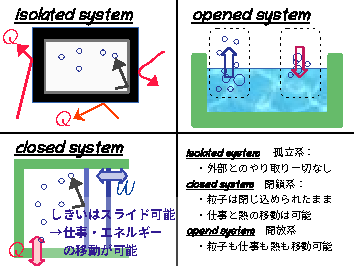
\includegraphics[keepaspectratio, width=7.5cm,height=6.9cm,clip]{neturikigaku_kankyo1.pdf}
                \caption{系の分類}
                \label{fig:neturikigaku_kankyo1}
            \end{center}
        \end{figure}

    \subsection{外界}
        着目している毛糸直接または間接的に接していて,熱や仕事,物質をやり取りする物質系を \textbf{外界} という.

    \subsection{環境}
     考察対象となる熱力学の系が置かれた周囲の状況のうち,
     室温や大気圧,熱湯(熱源)といった外界の条件をさして,これらを \textbf{環境} という.

    \subsection{拘束}
        考察対象となる熱力学の系が置かれた周囲の状況のうち,
        容器の壁やしきり,ピストンやピストンのストッパーといった,形状や体積および物質量を決める拘束条件,及び,
        断熱材や半透膜といった熱や物質の透過性を決める境界の性質,これらを \textbf{拘束} という.

    \subsection{環境と拘束}
        巨視的な系の熱平衡状態は,環境と拘束の下で,実現している.環境や拘束の変化に応じて,
        系の熱平衡状態は変化する.

    \subsection{可逆変化・非可逆変化}
        状態変化させた後で,対象とする系とその外界も含めてもとの状態に戻せる変化のこと
        を \textbf{可逆変化} という.系だけがもとに戻っ多としても,可逆変化とはいわない.
        逆に,状態を戻せない変化のことは,\textbf{非可逆変化} という.

    \subsection{断熱環境:断熱ポットの中の熱湯}
        ポットの内部には,水蒸気と空気の混合系(気体)と水の単一系(液体)の2つの部分系からなっている.
        それぞれの部分系は均質である.ポットは閉じていて,形状が固定されていることから,系の物質量と体積は
        一定に保たれている.系は熱を通さない材質の壁(\textbf{断熱壁})で囲まれていて,ポットの外部の大気の
        熱のやり取りができない.そのため,系の温度は外部の温度に影響されずに,一定の温度に保たれている.
        一方,2つの部分系(水と水蒸気・空気)の間には仕切りがなく,熱や物質を自由にやり取りできる.

        断熱ポット全体を見れば,孤立系である.内部の水と水蒸気と空気に着目すると,相互に粒子やエネルギーの
        やり取りが行えるため,個々の水と水蒸気は開放系である.
        \begin{figure}[hbt]
            \begin{center}
                \includegraphicsdefault{neturikigaku_danetu_pot.pdf}
                \caption{断熱ポット}
                \label{fig:neturikigaku_danetu_pot}
            \end{center}
        \end{figure}

    \subsection{透熱環境:シリンジの中に封入された気体}
        シリンジの内部は均質な気体の系である.ピストンとゴム栓で閉じていることで,気体の物質量は一定に保たれている.
        ピストンが\textbf{可動}である場合,内部の気体は膨張あるいは収縮ができて,体積は変化する.ピストンをストッパー
        で固定する場合は,気体の体積を一定にする拘束が加わる.系の熱を通す材質の壁(\textbf{透熱壁}:シリンジとピストン)
        で囲まれており,内部の気体はシリンジの外部の大気と熱のやりとりができる.そのため,系の温度はシリンジの外部の
        温度と等しくなる.シリンジの外部の温度・圧力は,室温・大気圧に保たれている.
        \begin{figure}[hbt]
            \begin{center}
                \includegraphicslarge{netsurikigaku_toukaheki.pdf}
                \caption{透熱壁}
                \label{fig:netsurikigaku_toukaheki}
            \end{center}
        \end{figure}

    \subsection{熱源:浴槽ないの大量の熱湯の中に置かれた鉄球}
        十分多い量の熱湯の中に小さな手球をいれた系を考える.
        熱湯と鉄球は,それぞれ均質な部分系である.鉄球は変形したり傷がついたりしないものとすれば,
        この部分の体積・物理量は一定に拘束されている.熱湯は蒸発することができ,膨張することもできる
        ので,この部分系の体積と物質量に拘束はない.鉄球と熱湯は直接的に接しているため,熱のやりとりが
        あり,その結果,どちらも温度が変わる.

        熱湯の量が十分に多く,鉄球との熱のやりとりによる温度変化が認められないとき,お湯は鉄球に対して熱の
        供給源とみなせる.これを \textbf{熱源}(\textbf{熱浴})という.ただし,大気と熱のやりとりによって
        お湯は冷めていく.一定の熱の供給源として用いるためには,湯沸かし器などによって,お湯の温度を一定に
        保つ必要がある.
        \begin{figure}[hbt]
            \begin{center}
                \includegraphicslarge{netsurikigaku_netugen.pdf}
                \caption{熱源/熱浴}
                \label{fig:netsurikigaku_netugen}
            \end{center}
        \end{figure}


    \subsection{半透膜:半透膜でしきられた希薄溶液}
    ある液体に少量の物質を溶かして作った溶液を \textbf{希薄溶液} という.溶けている物質を \textbf{溶質} といい,
    溶かすために用いる液体を \textbf{溶媒} という.また,溶媒は透過するが溶質は透過しないような膜状の物質を \textbf{半透膜} という.

    ビーカー内を半透膜で2つに仕切り,片方には溶媒のみを,もう片方には溶質と溶媒を入れる.十分時間が経過した後,ビーカー内の気迫溶液の系は,
    半透膜で仕切られた溶媒と溶質の混合系と,溶媒のみ系の2つの均質な系からなる.溶質の物質量は半透膜によって片側の系(混合系)に拘束されている.
    溶質の物質量は2つの系の間で自由にやりとりができる.

    ビーカー内の希薄溶液とビーカー外の大気との境界にしきりはなく,熱や物質を自由にやり取りできる.外界の条件は室温で大気圧にある.
    \begin{figure}[hbt]
        \begin{center}
            \includegraphicsdefault{netsurikigaku_hantoumaku.pdf}
            \caption{半透膜}
            \label{fig:netsurikigaku_hantoumaku}
        \end{center}
    \end{figure}

\section{絶対温度(気温計による定義)}
    \subsection{熱力学第0法則}
        系Aと系Bが熱平衡状態にあり,系Aと系Cが熱平衡状態にあるならば,系BとCも熱平衡状態にある.
        これは経験則で,実験事実である.熱力学の理論体系の基礎になる事柄なので,
        このことを \textbf{熱力学第0法則} といわれることも多い.ただ,熱力学の第1法則と第2法則に
        比べると,この第0法則という表現は少し非公式の感じがする.しかし,大事な原則の1つである.
        \begin{figure}[hbt]
            \begin{center}
                \includegraphicsdefault{netsu_heikou_law0.pdf}
                \caption{熱平衡(\textbf{熱力学第0法則})}
                \label{fig:netsu_heikou}
            \end{center}
        \end{figure}

    \subsection{温度}
        実際,透熱壁を介して,系Bと系Cを接触させてみると,温度など状態量に変化はなく,互いに熱平衡状態に
        あることがわかる.このように,1つの系を基準にして,他の2つの系が互いに熱平衡状態にあるかどうかを,
        直接接触させることなく判断できる.この熱平衡状態の性質は,\textbf{温度計} によって温度を定めることの
        できる原理的な理由になっている.系Aを温度計とみなせば,系Bと系Cは等しい温度にあるとえる.
        \begin{figure}[hbt]
            \begin{center}
                \includegraphicslarge{netsurikigaku_ondokei.pdf}
                \caption{温度計}
                \label{fig:netsurikigaku_ondokei}
            \end{center}
        \end{figure}

        温度の目盛りを決めるには,一般に,温度計に用いる物質の熱膨張の性質を利用する.
        ほとんどの物質は温度が高くなると体積が膨張し,温度が低くなると収縮する性質を持つ.
        熱膨張とは,温度による体積の膨張のことのことである.

        温度計に用いる物質は何でも良い.昔は(昭和,平成初期),実用的には水銀やアルコールが使われていた.
        水の凝固点(0[\circC])のときの物質の体積を${V}_{0}=$,また,
        水の沸点(100[\circC])のときの物質の体積${V}_{100}=$として,
        その差${V}_{100}-{V}_{0}$を100等分して目盛りを作る.
        このように考えた場合,温度$t$体積$V$の関数として現すことができて($t=t(V)$),
        \begin{equation}
            t(V) := 100 \times \frac{V-{V}_{0}}{{V}_{100}-{V}_{0}}
        \end{equation}
        とかける.
        逆に,温度が分かれば,体積もわかる.

    \subsection{絶対温度}
        気体は,十分に希薄でれば,その体積の膨張率は一定とみなせる.
        \begin{align}
            V &= {V}_{0} + \frac{{V}_{0}}{273.15}t  \notag \\
              &= {V}_{0}\left( 1 + \frac{1}{273.15}t \right) \notag \\
              &= {V}_{0}\left(  \frac{273.15 + t}{273.15} \right)
        \end{align}
        シャルルの法則の一例である.

        ここで,
        \begin{equation}
            T := 273.15 + t
        \end{equation}
        となる温度を新たに定義する.これを \textbf{気体温度計による絶対温度} という.すると,
        \begin{equation}
            V(T) = {V}_{0} \frac{T}{273.15} = \frac{{V}_{0}}{273.15}T
        \end{equation}
        となり,単純な比例の式になった.



%===================================================================================================
%  Chapter : 気体の状態方程式
%  説明    : ボイルの法則,シャルルの法則から,気体の状態方程式を導く
%===================================================================================================
\chapter{気体の状態方程式}
%   %-----------------------------------------------------------------------------------------------
%   %  Input
%   %    File Name : PhysNote_ST_StatGasEq.tex
%   %    説明      : 気体の状態方程式を導く
%   %-----------------------------------------------------------------------------------------------
        %       %======================================================================
%       %  Section
%       %======================================================================
        \section{ボイルの法則}
            近代科学の先駆者としてコペルニクス
                \footnote{
                    Nicolaus Copernicus (1473--1543,?):地動説を唱えたことで有名.
                    地球は太陽を中心に公転しているのだ.
                }
            やガリレイがよく挙げられる.
            それ以前には,思考のみによって世界の真理を追求してきたのだが,
            彼らは,これに疑問を訴え,観察や実験を通した事実を基に,世界の真理を
            追求すべきだと主張した.

            ボイル
                \footnote{
                    Robert Boyle (1627--1691,イギリス):化学者,物理学者.
                }
            もその考えに基づき, \textbf{自然を実験と観察に基づいて考える} という理念の下で,
            主に化学現象に関する研究を行っていた.
            その中で,ボイルは気体に関する法則を
            実験的に見出した.\textbf{ボイルの法則} である.
                \begin{myshadebox}{ボイルの法則}
                    温度を一定に保っている状態では,圧力と体積は反比例の関係にある.
                    言い換えると,圧力と体積の積は一定値を保つ.
                    圧力を $p$,体積を $V$ としたとき,
                    \begin{align}
                        pV = k. \mbox{(温度一定)}
                    \end{align}
                    ここで,$k$ は気体の初期状態により決まる定数.
                \end{myshadebox}

            ボイルの法則や,この後に説明するシャルルの法則は,熱力学の教科書だけでなく,
            化学の教科書にも登場する.その意味で,熱力学と化学を結ぶ重要な法則である.


%       %======================================================================
%       %  Section
%       %======================================================================
        \section{シャルルの法則}
            シャルル
                \footnote{
                    Jacques Alexandre C\'{e}sar Charles (1746--1823):化学者.
                }
            気体に関する法則を実験的に見出した.\textbf{シャルルの法則} とよばれる.
                \begin{myshadebox}{シャルルの法則}
                    圧力を一定に保っている状態では,体積と温度は比例関係にある.
                    言い換えると,体積と温度の比は一定値を保つ.
                    体積を $V$,温度を $T$ としたとき,
                    \begin{align}
                        \frac{V}{T} = l. \mbox{(圧力一定)}
                    \end{align}
                    ここで,$l$ は気体の初期状態により決まる定数.
                \end{myshadebox}

            比例定数についても実験的に得られる.もう少しシャルルの法則を詳しく書くと,
            次よようになる.すなわち,\textbf{一定圧力において,気体の体積は,
            温度を1度上昇させると,0度の時の体積の1/273ずつ増加する}.
            式で表すと,0度の時の体積を ${V}_{0}$ とし,温度t度上昇させた時の,気体の体積 $V(t)$ は,
                \begin{equation*}
                    V(t) = \frac{1}{273} {V}_{0}t + {V}_{0}.
                \end{equation*}
            次のように式変形してみよう.
                \begin{equation*}
                    V(t) = \left( \frac{1}{273}t + 1 \right) {V}_{0} = \frac{t+273}{273} {V}_{0}.
                \end{equation*}
            $T=t+273$ を導入して,
                \begin{equation*}
                    V(t) = \frac{T}{273} {V}_{0}
                \end{equation*}
            となる.この $T$ のことを \textbf{絶対温度} といい,単位を [K] で表す.
            [K] は「ケルビン」と読む.
                \begin{figure}[hbt]
                    \begin{center}
                        \includegraphicsdefault{charlesNohousoku.pdf}
                        \caption{シャルルの法則}
                        \label{fig:charlesNohousoku}
                    \end{center}
                \end{figure}


%       %======================================================================
%       %  Section
%       %======================================================================
        \section{ボイル$=$シャルルの法則}
            ボイルの法則とシャルルの法則を1つにまとめることができる.
            ひとまとめにできることを示すには,実際に状態遷移の計算をしてみて,
            矛盾がないことを確認すればいい.

            温度 $T$ と体積 $V$ と圧力 $p$ の添字のアルファベット(A, B, C)は,
            図\ref{fig:BoyleCharlesTotal1111}で示す状態に対応する.
            状態遷移は次のように行う.まず,最初の状態をAとする.状態Aから
            等温変化させて,状態Bへ移す.この時,等温変化であるから,ボイルの
            法則が成り立つはずである.更に,状態Bから状態Cへ等圧変化により
            遷移させる.この場合は,等圧変化であるので,シャルルの法則が
            成り立つはずである.最後に,状態Aと状態Cにおける各温度,体積,圧力
            の関係が等しければ,ボイルの法則とシャルルの法則をひとまとめに
            できることが示される.
            \begin{figure}[hbt]
                \begin{center}
                    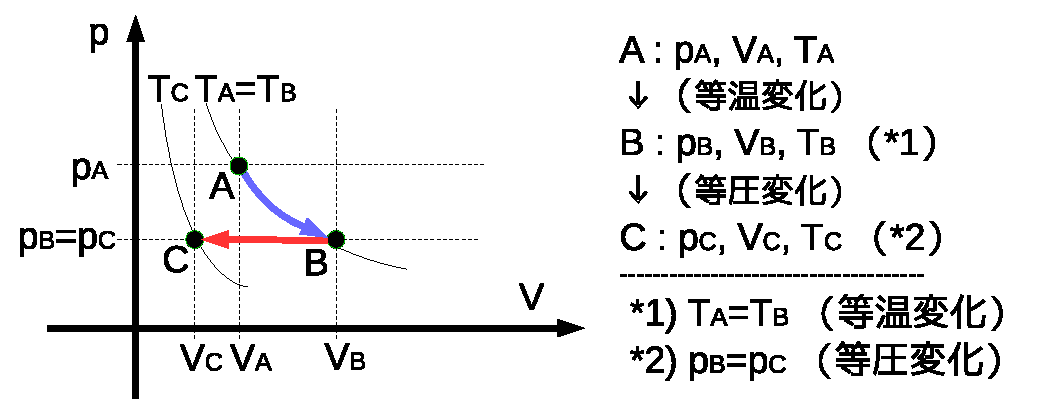
\includegraphics[keepaspectratio, width=8.0cm,height=3.3cm,clip]{BoyleCharlesTotal1111.pdf}
                    \caption{ボイル$=$シャルルの法則}
                    \label{fig:BoyleCharlesTotal1111}
                \end{center}
            \end{figure}

            一定温度 $T_{A}$ の下で,ボイルの法則により,
                \begin{equation*}
                    {p}_{A}{V}_{A} = {p}_{B}{V}_{B}.
                \end{equation*}
            後の式変形のため,${V}_{B}$ について解いておく.
                \begin{equation*}
                    {V}_{B} = \frac{{p}_{A}{V}_{A}}{{p}_{B}}.
                \end{equation*}

            引き続き,一定圧力 $p_{B}$ の下で,シャルルの法則より,
                \begin{equation*}
                    \frac{{V}_{B}}{{T}_{B}} = \frac{{V}_{C}}{{T}_{C}}.
                \end{equation*}
            ${V}_{B}$ を置き換えて,
                \begin{equation*}
                    \frac{{p}_{A}{V}_{A}}{{T}_{B}{p}_{B}} = \frac{{V}_{C}}{{T}_{C}}.
                \end{equation*}
            両辺に ${p}_{B}$ をかけておく.
                \begin{equation*}
                    \frac{{p}_{A}{V}_{A}}{{T}_{B}} = \frac{{p}_{B}{V}_{C}}{{T}_{C}}.
                \end{equation*}

            ここで,状態AからBの遷移は等温変化であるので,
                \begin{equation*}
                    {T}_{B} = {T}_{A}.
                \end{equation*}
            また,状態Bから状態Cへの遷移は等圧変化であるので,
                \begin{equation*}
                    {p}_{B} = {p}_{C}.
                \end{equation*}
            この2点を考慮すると
                \begin{equation*}
                    \frac{{p}_{A}{V}_{A}}{{T}_{A}} = \frac{{p}_{C}{V}_{C}}{{T}_{C}}.
                \end{equation*}
            式の添字に着目すれば,最初の状態Aと最後の状態Cにおいて,
            関係式 $pV/T$ が同じ値をとることがわかる.この値を $k$ と書くことにすれば
                \footnote{
                    \begin{equation*}
                        k := \frac{{p}_{A}{V}_{A}}{{T}_{A}} = \frac{{p}_{C}{V}_{C}}{{T}_{C}}.
                    \end{equation*}
                },
                \begin{equation*}
                    \frac{pV}{T} = k.
                \end{equation*}
            次のように書き換えれば,よく見かける方程式になる.
                \begin{equation*}
                    pV=kT.
                \end{equation*}
            これが,\textbf{ボイル$=$シャルルの法則} である.
            ボイル$=$シャルルの法則の式は,\textbf{気体の状態方程式} とよばれる.

            まとめておこう.
                \begin{myshadebox}{ボイル$=$シャルルの法則}
                    気体において,温度 $T$,体積 $V$,圧力 $p$ は,
                    定数 $k$ を用いて,以下の関係式を満たす.
                    \begin{align}
                        pV=kT.
                    \end{align}
                \end{myshadebox}

%       %======================================================================
%       %  Section
%       %======================================================================
        \section{理想気体}
        理想気体の状態方程式が厳密に成り立つ理想的な気体のことを \textbf{理想気体} という.
        理想気体は実在しないが,高温状態あるいは低圧状態では,実在する気体を理想気体と
        みなしうることができる,ということもある.実際は,工学的には,理想と現実の乖離具合
        を常に意識しなければならない.ただ,理論構築のためには,理想気体はとても
        有用なので,熱力学では理想気体が主役になる.理想気体の性質を理論的に把握することで,
        現実に存在する \textbf{実在気体} の性質を推察できるようになる.
        どれだけ実在気体が理想気体と乖離しているかが,実在気体の特徴であるともいえる.

%       %======================================================================
%       %  Section
%       %======================================================================
        \section{状態方程式}
        \begin{mycomment}
            気体が従う自然法則(方程式)を導入する.
            熱力学では,ニュートンの運動方程式と同じように,天下り的に与えられる式であり,他から導き出されるものではない.
            気体を無数の粒子の集まりとして仮定した統計力学から,理想気体の状態方程式を導けるが,これは熱力学の論理の範囲外である.
            今は熱力学を学習しているため,状態方程式は実験事実の自然法則として受け入れよう.
        \end{mycomment}
        \subsection{理想気体の状態方程式}
        状態方程式は熱力学の基本法則の1つである.以下に書き下そう.
        \begin{myshadebox}{理想気体の状態方程式}
            理想気体において,圧力$P$[N/m${}^{2}$],体積$V$[m${}^{3}$],物質量$n$[mol], 温度$T$[K],
            気体定数$R$[J/mol$\cdot$K]の条件下で,以下が成り立つ.
            \begin{equation}
                PV = nRT.
            \end{equation}
        \end{myshadebox}

        理想気体の状態方程式のことは,混乱の恐れがない場合には,単に,状態方程式ともいう.

        \subsection{気体の濃度}
        体積$V$[m${}^{3}$]の容器の中に$n$[mol]の気体が入っているとき,この気体の濃さを
        数値化できる.同じ堆積中で,たくさん気体が入っていれば濃くなるし,少なければ,
        薄くなる.これを \textbf{濃度} という.濃度を$\sigma$で現すと,
            \begin{align}
                \sigma = \frac{n}{V}
            \end{align}
        である.状態方程式と対比させてみと,以下になる.
            \begin{align*}
                 PV &= nRT \\
                \Leftrightarrow P &= \frac{n}{V}RT \\
                \Leftrightarrow P &= \sigma RT \\
            \end{align*}

        濃度$\sigma = n/V$が一定の場合に成立する式だ.圧力は濃度に比例する.
        気体の濃度が濃いほど圧力は高くなるのだ.
        \begin{align}
            P(T) = \sigma RT.
        \end{align}

        注意すべきは式を濃度$\sigma$について解いてみて
        \begin{align}
            \sigma = \frac{P}{RT}
        \end{align}
        としてしまうと,あたかも濃度が圧力に比例するようにみえる.この解釈は間違いである.
        濃度はもともと,$n/V$であることを忘れてはいけない.$n$の値は変化しない(急に気体が湧いて出たりしない).
        つまり,圧力が変化して濃度が変わったのであれば,実際には体積$V$が変化したということである.
        圧力$P$を高くして体積$V$をぐぐっと縮みることで,濃度が高くなるのだ.

        \subsection{実在気体の状態方程式}
        \subsubsection{ビリアル方程式}
        \subsubsection{ファンデルワールスの状態方程式}
        実在する気体の振る舞いをいい感じに表現する方程式がある.液体にも適用可能である.
        ファンデルワールス
            \footnote{
                Johannes Diderik van der Waals(1837--1923,オランダ):ヨハネス ディーデリク ファン デル ワールス.
                1910年にこの気体の状態方程式の発見によりノーベル賞を受賞している.分子間力の1つである,
                \textbf{ファンデルワールス力}(\textbf{ファンデルワールス結合})でもその名前が知られている.
            }というオランダ人の物理学者が提案した,実在気体の状態方程式である.
        気体の種類によって,振る舞いが異なるので,それに対応する特徴的な 定数$a$,$b$が使われる.

        ファンデルワールスの状態方程式も他から導かれるものではないが,雰囲気からなら説明・導入ができる.
        理想気体の状態方程式に現実的要素を織り交ぜて,変形していく.理想気体からの乖離を補正するのである.
        補正を受けるのは,体積$V$と圧力$P$である.まず,体積から考えよう.

        理想気体を構成する粒子は体積はないものと仮定されていた
            \footnote{
                実際,熱力学が成立した時代にも,原子や分子の存在は知られていなかった.
                確かに,デモクリトストスが提唱していたと言われているが,空想上の概念であり,
                デモクリトスが実験的に原子や分子の存在を確かめたわけではない.
            }.
        しかし,実在気体を構成する粒子は,一つ一つは微小であるが,体積を持つ.
        現実気体$n$[mol]の体積を${V}_{R}$(RealのR),おなじく理想気体$n$[mol]の体積を${V}_{I}$(ImageのI)とするならば,
        体積の補正項を$b$を導入して,
            \begin{equation}
                {V}_{R} = {V}_{I} + bn
            \end{equation}
        と書ける.実在気体の体積は理想気体の体積よりも,粒子自体の大きさ分だけ,大きいと考える.
        \begin{figure}[hbt]
            \begin{center}
                \includegraphicsmiddle{netsurikigaku_van_der_waals_force.pdf}
                \caption{実在気体:体積}
                \label{fig:netsurikigaku_van_der_waals_force}
            \end{center}
        \end{figure}

        実在の気体の圧力も理想とは異なる.実際には分子を構成する原子機構により分子内部の電子の位置が偏り,
        分子自体に正負の電気的な偏りができる.これが複数存在すると,分子のプラス側(正)と別の分子のマイナス側(負)が
        引き合う現象がおきる.これを \textbf{分子間力} という
            \footnote{
                分子間力といっても,発生機構によって細分化される.イオン間相互作用,水素結合,双極子相互作用,ファンデルワールス力.
            }.
        分子間力が働くと,分子の運動が束縛されて(分子の運動が鈍くなり),結果,圧力が弱まる.
        \begin{figure}[hbt]
            \begin{center}
                \includegraphicsmiddle{netsurikigaku_van_der_waals_force2.pdf}
                \caption{実在気体:圧力}
                \label{fig:netsurikigaku_van_der_waals_force2}
            \end{center}
        \end{figure}
        では,どの程度弱まるのか.モル濃度の2乗に比例すると考えられている(根拠は実験かな).
        現実気体$n$[mol]の圧力を${P}_{R}$(RealのR),おなじく理想気体$n$[mol]の圧力を${P}_{I}$(ImageのI)とするならば,
        圧力の補正項を$a$を導入して,
        \begin{equation}
            {P}_{R} = {P}_{I} - a{\left( \frac{n}{{V}_{I}} \right)}^{2}
        \end{equation}
        となる.

        理想気体の状態方程式は厳密に成り立つ.${V}_{I}$と${P}_{I}$を使って理想気体の状態方程式を書くならば,
        \[
            {P}_{I}{V}_{I} = nRT.
        \]
        だけど,${V}_{I}$と${P}_{I}$は実在気体の体積と圧力だから,この式は間違っている.式を補正して正しくしよう.
        この理想気体型の状態方程式に,さっき計算した結果を適用すればよい.
        まず,上記の2つの式をそれぞれ,${V}_{I}$と${P}_{I}$について解くと,
        \begin{align}
            {V}_{I} &= {V}_{R} - bn \\
            {P}_{I} &= {P}_{R} + a{\left( \frac{n}{{V}_{I}} \right)}^{2}
        \end{align}
        である.これを状態方程式に代入しよう.
        \begin{equation}
            \left( {P}_{I} + a{\left( \frac{n}{{V}_{I}} \right)}^{2} \right) \left( {V}_{I} - bn \right) = nRT.
        \end{equation}
        カッコが多くてきたないので,適当に外すと,
        \begin{equation}
            \left( {P}_{I} + a\frac{{n}^{2}}{{{V}_{I}}^{2}} \right) \left( {V}_{I} - bn \right) = nRT.
        \end{equation}
        となる.

        これを \textbf{ファンデルワールスの状態方程式} という.
        また,$a$,$b$のことを \textbf{ファンデルワールス定数} という.
        \begin{myshadebox}{ファンデルワールスの状態方程式}
            現実気体$n$[mol]の圧力を${P}_{I}$,現実気体$n$[mol]の体積を${V}_{I}$として(RealのR),
            \begin{equation}
                \left( {P}_{I} + a\frac{{n}^{2}}{{{V}_{I}}^{2}} \right) \left( {V}_{I} - bn \right) = nRT.
            \end{equation}
        \end{myshadebox}

        「理想気体の圧力に対して,実在気体の圧力は分子間力の分だけ小さくなるので,補正項を足す」,
        「理想気体の体積に対して,実在気体の体積は大きさがある分だけ大きくなるので,補正項を引く」
        と捉えておけばよいだろう.

        ちなみに,教科書には${P}_{I}$を左辺にした表現となっていた.
        \begin{equation}
             {P}_{I}  =  \frac{nRT}{\left( {V}_{I} - bn \right)} - a{\left(\frac{n}{{V}_{I}} \right)}^{2}.
        \end{equation}
        ちょっと細工すると,
        \begin{equation*}
            {P}_{I}  =  \frac{1}{\left( {V}_{I} - bn \right)}nRT - a{\left(\frac{n}{{V}_{I}} \right)}^{2}.
       \end{equation*}
        この表現からは,現実気体の圧力は,理想気体の$1/({V}_{I} - bn)$で,さらに,分子間力がはたらく分だけ
        小さくなることが読み取りやすい.

%       %======================================================================
%       %  Section
%       %======================================================================
        \section{分圧の法則}
        混合気体が入った容積の圧力を考える.この容積内部の圧力について,以下の法則が成り立っている.
        \begin{myshadebox}{分圧の法則}
            混合気体の圧力(全圧)は,それを構成する各々の種類の成分圧力(分圧)
            の和に等しい.気体は何種類もあってよくて,$k$種類の気体がある場合は
            以下の式が成り立つ.
            \begin{equation}
                P = \sum_{i=1}^{k} {p}_{i}
            \end{equation}
            左辺の$P$が全圧であり,右辺の${p}_{i}$($i=1,\,2,\,\cdots,\,n$)が分圧である.
        \end{myshadebox}
        ドルトンが提唱した法則なので,「ドルトンの分圧の法則」とかと紹介されることも多い.

        \begin{figure}[hbt]
            \begin{center}
                \includegraphicsmiddle{netsurikigaku_bunsi_undo_ron_bunatsu.pdf}
                \caption{全圧と分圧}
                \label{fig:netsurikigaku_bunsi_undo_ron_bunatsu}
            \end{center}
        \end{figure}

        う〜ん,この法則はどうやって実験的に確かめたのだろうか.
        原理的には,こうだろう.まず,同体積の気体A,B,Cを用意して,
        それぞれの圧力の計測する.これは,後で気体を混合した場合に,元々の各気体の分圧の測定とみなせる.
        その結果をそれぞれ${P}_{A}$,${P}_{B}$,${P}_{C}$であったとしよう.
        次に,同じ体積ににA,B,Cの3つの気体を同じ一つの箱に押し込めて,圧力を測定する.
        たとえば,BとCをAの箱に詰めるなど.そうすると,3種類の全気体が1箇所に集まることになり,
        このAとBとCから構成される全気体の圧力(すなわち全圧)の測定が可能になる.
        分圧の法則にしたがえば,全圧を単に$P$すると,
            \[
                P = {P}_{A} + {P}_{B} + {P}_{C}
            \]
        と計算できる.

        気体が分子から構成されていることと理想気体の状態方程式から,分圧の法則が導けないだろうか.
        もう少し遊んでみよう.
        
        状態方程式$PV=nRT$から,$P=(n/V)RT$.温度$T$は一定であるとする.すると,
        \[
            \frac{n}{V}RT = \frac{{n}_{A}}{{V}_{A}}RT + \frac{{n}_{B}}{{V}_{B}}RT + \frac{{n}_{C}}{{V}_{A}}RT.
        \]
        ${n}_{A}$,${n}_{B}$,${n}_{C}$はA,B,Cのそれぞれのモル数.
        ${V}_{A}$,${V}_{B}$,${V}_{C}$はそれぞれ,A,B,Cの体積である.体積は同じで,
        \[
            V = {V}_{A} = {V}_{B} = {V}_{C}.
        \]
        だから,
        \begin{align*}
            \frac{n}{V}RT &= \frac{{n}_{A}}{V}RT + \frac{{n}_{B}}{V}RT + \frac{{n}_{C}}{V}RT.
        \end{align*}
        気体の単位体積あたりのモル数(濃度)$\sigma$を考えて,
        \[
            {\sigma}     :=\frac{n}{V},       \quad {\sigma}_{A} :=\frac{{n}_{A}}{V}, \quad
            {\sigma}_{B} :=\frac{{n}_{B}}{V}, \quad {\sigma}_{C} :=\frac{{n}_{C}}{V}
        \]
        と書くことにすると,
        \begin{align*}
                            {\sigma} RT &= {\sigma}_{A} RT + {\sigma}_{B} RT + {\sigma}_{C} RT \\
            \Leftrightarrow {\sigma}    &= {\sigma}_{A}    + {\sigma}_{B}    + {\sigma}_{C}.
        \end{align*}
        となる.体積が一定であれば,それぞれの気体を混ぜ合わせた後の濃度は,それぞれの
        濃度の足し算で計算できる.体積$V$がみえるようにかくと,
        \begin{align*}
                          {\sigma} &= {\sigma}_{A}     + {\sigma}_{B}      + {\sigma}_{C} \\
                       \frac{n}{V} &= \frac{{n}_{A}}{V} + \frac{{n}_{B}}{V} + \frac{{n}_{C}}{V} \\
            \therefore           n &= {n}_{A} + {n}_{B} + {n}_{C}
        \end{align*}
        である.容積中の全体の気体のモル数は,個々の気体のそれぞれのモル数を足し合わせたものである.

        このモル数の足し合わせの結果をベースにして,温度と体積が一定であるという条件の下で,
        これまでの議論を逆にたどれば,分圧の法則が導ける.
        \begin{align*}
                                        n &= \sum_{i=1}^{k} {n}_{i}\\
            \Leftrightarrow \frac{n}{V}   &= \frac{1}{V}\sum_{i=1}^{k} {n}_{i} = \sum_{i=1}^{k} \frac{{n}_{i}}{V}\\
            \Leftrightarrow \frac{n}{V} T &= \left(\sum_{i=1}^{k} \frac{{n}_{i}}{V}\right)  T = \sum_{i=1}^{k}\left( \frac{{n}_{i}}{V} T\right)\\
            \Leftrightarrow \frac{n}{V}RT &= \left(\sum_{i=1}^{k} \frac{{n}_{i}}{V}\right) RT= \sum_{i=1}^{k}\left( \frac{{n}_{i}}{V}RT\right)  \\
            \Leftrightarrow             P &= \sum_{i=1}^{k} {p}_{i}.\quad\mbox{(分圧の法則が導けた)}\
        \end{align*}
        どちらかと言うと,モル数をベースにしたほうが直感的で理解しやすいと思う.ただ,式変形に物理的な洞察はなく,説得力に欠ける.
        モル数をベースにして,温度と圧力が一定だったら,必然的に,分圧の法則が成り立つ,という事実が説明できるだけだ.





\chapter{気体分子運動論}
%   %-----------------------------------------------------------------------------------------------
%   %  Input
%   %    File Name : PhysNote_GasMolTheory.tex
%   %    説明      : 気体分子運動論を学習する.気体は多数の微粒子の集まりとして考える
%   %-----------------------------------------------------------------------------------------------
        %   %==========================================================================
%   %  Comment
%   %==========================================================================
\begin{mycomment}
    気体についての考察.気体は無数の分子から構成されていると言う仮定して,
    気体の圧力や分子の運動エネルギーについて調べてみよう.
\end{mycomment}

\section{仮定}
    気体分子運動論を考える状況について,議論の最初に,いくつか仮定を設けておく.
    \begin{itembox}[l]{気体分子運動論の仮定}
        \begin{itemize}
            \item 気体は理想気体を対象とし,分子間力は考えない
            \item 分子は数え切れないほど多く存在し,巨視的に見れば,
                  あらゆる方向に均一に運動している($x$,$y$,$z$の全方向に均一である)
            \item 分子同士の衝突はないものとする(衝突しても結果は変わらないが,状況が複雑になり計算が面倒になる)
            \item 分子と壁は弾性衝突する(衝突係数$=1$:跳ね返りによるエネルギーの散逸なし)
            \item 重力の影響はないものとする
            \item 1辺が$L$[m]の立方体の容器に入った気体分子を考える(体積は$V={L}^{3}$[m${}^{3}$])
        \end{itemize}
    \end{itembox}

\section{分子の速度とその平均}
    まず,立方体のある1つの分子に着目する.
    この分子の速度を$\bv$とする.速度は3次元であるので,$\bv$は$x$,$y$,$z$成分に分解できる.
    \begin{equation}
        \bv = ({v}_{x},\,{v}_{y},\,{v}_{z}).
    \end{equation}
    他のベクトル量も3次元であり,速度と同様に3つの成分を持つ.
    後で使うので,速度の2乗平均$\bar{{v}^{2}}$も計算しておこう.

    まず,速度ベクトルを2乗する.
    \[
        {\bv}^{2} = {v}^{2} = {{v}_{x}}^{2} + {{v}_{y}}^{2} + {{v}_{z}}^{2}
    \]
    すべての分子の平均をかんがえると,
    \begin{align*}
        \bar{{\bv}^{2}} &= \bar{{v}^{2}} \\
                        &= \bar{{{v}_{x}}^{2} + {{v}_{y}}^{2} + {{v}_{z}}^{2}} \\
                        &= \bar{{{v}_{x}}^{2}} + \bar{{{v}_{y}}^{2}} + \bar{{{v}_{z}}^{2}}
    \end{align*}
    さらに,あらゆる方向に均一に運動しているので,
    \[
        \bar{{{v}_{x}}^{2}} = \bar{{{v}_{y}}^{2}} = \bar{{{v}_{z}}^{2}}
    \]
    としてよい.一旦${v}_{x}$だけの式にする.
    \[
        \bar{{v}^{2}} = 3\bar{{{v}_{x}}^{2}}
    \]
    これより,
    \begin{equation}
        \bar{{{v}_{x}}^{2}} = \frac{1}{3} \bar{{v}^{2}}
    \end{equation}
    を得る.この速度の式は後の計算で使うことになる.

    \begin{memo}{$N$個の分子の速度の2乗平均}
        この部分の計算で,現れた速度の2乗平均の計算方法を確認しておこう.
        $N$個の分子に,1から$N$の自然数で番号付けをしておこう.そして,
        $N$個の各々の分子の速度を,${v}_{i}$としよう.添字の$i$は1から$N$までの
        いずれかの自然数である.自然数$i$をきめると,対応する分子が定まるこのとになる.
        平均とは全部(ここでは$N$個)のデータを合計して,その総数(ここでは$N$個)で割った
        値のことである.${v}_{1}$,${v}_{2}$,${v}_{3}$,$\cdots$ の値はそれぞれ異なる.
        個々の値には興味はなく,その平均が知りたい.ここで知りたいのは速度の大きさの
        平均である.速度は正負の向きを持ったベクトルなので,このまま足し合わせても
        速さの平均値を求めることはできない
            \footnote{
                極端な例を上げよう.速度には正負の向きがあるため,
                たまたま,すべてを合計したら0になるかのせいもある.
                平均の速度が0となる.ベクトルとしてはそれで正解であるが,
                速さの平均を求めたいのであるから,平均が0になっていしまうのは困る.
                各々の絶対値をとる方法も考えれるかもしれないが,二乗して必ず正の値に
                なるように細工したほうが都合が計算しやすいし,式も見やすいし良い.
                二乗しているので,計算の最終段階で平方根を求めれば良い.
            }.
        そこで,速度の2乗平均を計算することにしよう.実は,運動エネルギーも速度の
        2乗でであるため,この方法が都合が良い.

        すると,速度の2乗平均は以下のように計算される.
        \begin{align*}
            \bar{{\bv}^{2}} &= \frac{1}{N} \left( {{\bv}_{1}}^{2} + {{\bv}_{2}}^{2} + \cdots + {{\bv}_{N}}^{2} \right ) \\
                            &= \frac{1}{N} \sum_{i=1}^{N} {{\bv}_{i}}^{2}.
        \end{align*}

        速さが知りたかったら,平方根取ればいい.
        \[
            v = \sqrt{\bar{{\bv}^{2}}} = \sqrt{\frac{1}{N} \sum_{i=1}^{N} {{\bv}_{i}}^{2}}.
        \]
    \end{memo}

    \section{分子1つが壁に衝突するときに,壁に与える平均の力:$\bar{{f}_{x}}$}
    まずは$x$軸方向のみを考えよう.
    \begin{figure}[hbt]
        \begin{center}
            \includegraphicslarge{netsurikigaku_bunsi_undo_ron.pdf}
            \caption{気体分子運動論}
            \label{fig:netsurikigaku_bunsi_undo_ron}
        \end{center}
    \end{figure}

    最初に,「壁が分子から受ける力積」を計算する.この力積を${I}_{x}$とする.
    計算したいのだが,壁の速度に変化がないので,壁の運動から直接的に計算できない.
    そこで,分子と壁の作用反作用の法則を利用する.つまり,
        \[
            \mbox{分子の受ける力積} = - \mbox{壁の受ける力積}
        \]
    が成り立っているはずなので,分子の受ける力積を計算して,符号を反対にすればよい.
    力積は運動量の変化分に等しく,
        \[
            \mbox{力積} = \mbox{衝突後の運動量} - \mbox{衝突前の運動量}
        \]
    である.運動量$m{v}_{x}$で運動していた分子は壁に衝突すると,速度は反対向きになり,$m(-{v}_{x})$となる.
    また,分子が壁から受ける力積は$x$軸方向の反対なので,符号はマイナスである.
    これに当てはめると,分子が壁から受ける力積$-{I}_{x}$は
    \begin{align*}
        - {I}_{x}   &= - \bar{{f}_{x}}  t     \\
                    &= m(-{v}_{x}) - m{v}_{x} \\
                    &= -m{v}_{x} - m{v}_{x}   \\
                    &= -2m{v}_{x}
    \end{align*}
    である.$\bar{{f}_{x}}$は一回の衝突で与える$x$方向の力の大きさである.
    これより,壁が分子から受ける力積${I}_{x}$は,
    \begin{equation}
        {I}_{x} = \bar{{f}_{x}}  t = 2m{v}_{x}
    \end{equation}
    となる
        \footnote{
            ちなみに,「壁が分子から受ける力積」を言い換えれば,「分子が壁に与える力積」である.
            言葉の表現による注意も怠りなく.
        }.

    次に,「1つの分子が$t$秒間に壁に与える力積」を計算する.壁にあたった瞬間を$t=0$としたとき,
    分子は往復で$2L$の距離を速度${v}_{x}$で運動しているわけだから,次に衝突する時間を$t'$とすれば,
    \[
        2L = {v}_{x}t'
    \]
    が成立している.$t'$について解いて,
    \[
        t' = \frac{2L}{{v}_{x}}
    \]
    としておこう.分子が壁に1回衝突するのにかかる時間が$t'=2L/{v}_{x}$であることがわかった.
    であれば,$t$秒間に衝突する回数$n$は,$t/t'$を計算すればよく,
    \[
        n = \frac{t}{t'}=\frac{t}{2L/{v}_{x}}=\frac{{v}_{x}t}{2L}
    \]
    となる.
    \begin{figure}[hbt]
        \begin{center}
            \includegraphicslarge{netsurikigaku_bunsi_undo_ron2.pdf}
            \caption{壁への衝突回数}
            \label{fig:netsurikigaku_bunsi_undo_ron2}
        \end{center}
    \end{figure}

    分子が壁に与える1回あたりの力積${I}_{x}$は${I}_{x} = \bar{{f}_{x}}  t = 2m{v}_{x}$であった.これを使えば,
    $t$秒間に分子1つが壁に与える力積がわかる.以下のとおりである.
    \[
        2m{v}_{x} \times \frac{{v}_{x}t}{2L}=\frac{m{{v}_{x}}^{2}}{L}t=\bar{{f}_{x}}  t.
    \]

    したがって,最後の等式の対応見れば,壁に与える平均の力$\bar{{f}_{x}}$がわかる.
    \begin{equation}
        \bar{{f}_{x}} = \frac{m{{v}_{x}}^{2}}{L}.
    \end{equation}

    \begin{figure}[hbt]
        \begin{center}
            \includegraphicsdefault{netsurikigaku_bunsi_undo_ron_rikiseki.pdf}
            \caption{力積}
            \label{fig:netsurikigaku_bunsi_undo_ron_rikiseki}
        \end{center}
    \end{figure}

    \section{分子N個が壁に衝突するときに,壁に与える平均の力:$\bar{{F}_{x}}$}
    分子$N$個の衝突によって,壁が受ける平均の力が知りたい.これは$\bar{{f}_{x}}$を$N$倍することで
    計算できる.ただし,注意が必要である.いままでは1つの分子について着目していたため,${{v}_{x}}^{2}$は
    確かな固定値であった.しかし,今回は$N$個の分子を対象にしており,すべての分子が一律に${{v}_{x}}^{2}$という
    速度で運動しているはずがなく,このまま${{v}_{x}}^{2}$すれば,誤りとなる.ではどうするかと言うと,
    答えは簡単で,$N$個の分子の速度の平均値を考えれば良い.これを$\bar{{{v}_{x}}^{2}}$とかくことにしよう.
    \begin{equation}
        \bar{{F}_{x}} = \frac{Nm\bar{{{v}_{x}}^{2}}}{L}.
    \end{equation}


    \section{気体の圧力:$P$}
    圧力とは,単位面積あたりの力のことであった.今の場合,面積は${L}^{2}$である.
    $N$個の分子からなる気体が発生させる圧力$P$は
    \[
        P = \frac{\bar{{F}_{x}}}{{L}^{2}} = \frac{Nm\bar{{{v}_{x}}^{2}}}{L{L}^{2}} = \frac{Nm\bar{{{v}_{x}}^{2}}}{{L}^{3}}
    \]
    である.ここで,${L}^{3}$は立方体の体積であるから,$V$という文字で置き換えておこう($V:={L}^{3}$).
    \[
        P = \frac{Nm\bar{{{v}_{x}}^{2}}}{V}
    \]
    さらに,さっき計算した速度の式
    \[
        \bar{{{v}_{x}}^{2}} = \frac{1}{3} \bar{{v}^{2}}
    \]
    を適用すると,
    \[
        P = \frac{Nm \left((\frac{1}{3} \bar{{v}^{2}}\right)}{V} =\frac{Nm\bar{{v}^{2}}}{3V}.
    \]
    となる.

    \section{分子1つの並進運動エネルギーの平均値}
    理想気体の状態方程式 $PV=nRT$に関連付けたいので,両辺に$V$をかけよう.
    \[
        PV = nRT =  \frac{Nm \left(\frac{1}{3} \bar{{v}^{2}}\right)}{V} =\frac{Nm\bar{{v}^{2}}}{3}.
    \]
    分子1つの運動エネルギーは$m\bar{{v}^{2}}/2$であるから,この式から抽出してみよう.
    $m\bar{{v}^{2}}/$について解いてから,両辺に$1/2$をかけるとよいだろう.
    \begin{align*}
                                   nRT &= \frac{Nm\bar{{v}^{2}}}{3} \\
        \Leftrightarrow m\bar{{v}^{2}} &= \frac{3nRT}{N} \\
        \Leftrightarrow \frac{1}{2}m\bar{{v}^{2}} &= \frac{3}{2} \frac{n}{N}RT.
    \end{align*}
    ここで,$n/N$に注目しよう.$N$は気体分子全部の個数で,$n$は物質量([mol])である.
    つまり,$N$を$n$で割ると,1[mol]あたりの分子の個数が計算できて,これはアボガドロ定数${N}_{A}$であり,
    \[
        {N}_{A} = \frac{N}{n}
    \]
    であるから,$n/N$を$1/{N}_{A}$で置き換えられる.
    \begin{align*}
        \frac{1}{2}m\bar{{v}^{2}} &= \frac{3}{2} \frac{R}{{N}_{A}}T.
    \end{align*}
    後で詳しく学習するが,$R/{N}_{A}$はボルツマン定数${k}_{B}$であり,以下を得る.
    \begin{equation}
        \frac{1}{2}m\bar{{v}^{2}} = \frac{3}{2} {k}_{B}T.
    \end{equation}
    分子の運動エネルギーの平均値は,絶対温度$T$のみにより定まり,気体種類には依存しないことがわかる.

    \section{単原子分子からなる理想気体の内部エネルギー}
    N個の単原子分子からなる理想気体の内部エネルギー$U$は,内部の分子の運動エネルギーの平均を$N$倍すればいい.
    \begin{align*}
        U &= N \times \frac{1}{2}m\bar{{v}^{2}} \\
          &= N \times \frac{3}{2} \frac{R}{{N}_{A}}T    \\
          &= \frac{3}{2} \frac{N}{{N}_{A}}RT
    \end{align*}
    ここで,$n=N/{N}_{A}$だから,
    \begin{equation}
        U = \frac{3}{2} nRT = \frac{3}{2} PV.
    \end{equation}
    単原子分子の内部エネルギーは絶対温度で定まり,絶対温度に比例する.

    考えなければならず,この結果は多原子分子には適用できない.
    \begin{figure}[hbt]
        \begin{center}
            \includegraphicslarge{netsurikigaku_bunsi_undo_ron_tangensibunsi.pdf}
            \caption{多原子分子の場合は回転の考慮も必要}
            \label{fig:netsurikigaku_bunsi_undo_ron_tangensibunsi}
        \end{center}
    \end{figure}


